%%
%%  Department of Electrical, Electronic and Computer Engineering.
%%  EPR400/2 Final Report - Main File.
%%  Copyright (C) 2011-2021 University of Pretoria..
%%  Template edited and improved by Marchant Fourie
%%

\documentclass{epr400}

%%%%%%%%%%%%%%%%%%%%%%%%%%%%%%%%%%%%%%%%%%%%%%%%%%%%%%%%%%%%%%%%%%%%%%%%%%%
%    ADD YOUR INFORMATION HERE                                            %
%%%%%%%%%%%%%%%%%%%%%%%%%%%%%%%%%%%%%%%%%%%%%%%%%%%%%%%%%%%%%%%%%%%%%%%%%%%

\eprtitle{Handwriting robot}
\eprcode{EPR400}
\eprcandidatename{D.R. Braune}
\eprstudentnumber{23539195}
\eprdate{November 2026}
\eprsupervisor{Prof. H.C. Myburgh}
\eprcopynum{Electronic copy}


\usepackage{amsmath}
\usepackage{nccmath}
\usepackage{lipsum}
\usepackage[hidelinks]{hyperref}
\usepackage{tabularx}
\usepackage{booktabs}
\usepackage{amssymb}
\usepackage{graphicx}
\usepackage{float}
\usepackage{listings}
\usepackage{tikz}
\usepackage{xcolor}
\usepackage{algorithm}
\usepackage{algorithmic}
\usetikzlibrary{arrows.meta,positioning,shapes.geometric,fit,calc,backgrounds}
\lstset{basicstyle=\ttfamily\small,breaklines=true,frame=single,numbers=none,columns=fullflexible,keepspaces=true}

%% ---------------------------------------------------------------------------
%%  Float packing.  Section 3 holds about 64 figures and tables, which saturates
%%  LaTeX's default float queue (at most 3 floats per page, and a float page
%%  need only be half full).  The queue then overflows and the deferred floats
%%  are dumped at the end of the section, far from the text that refers to them.
%%  Relaxing these limits packs the floats near their references and recovers
%%  the part-empty float pages.  It changes layout only, never content.
%% ---------------------------------------------------------------------------
%% Displayed equations: LaTeX's default skips are about 12 pt above and below,
%% which is generous for a report carrying well over a hundred of them.  6 pt
%% still separates a display clearly from its text.  Set here rather than per
%% file so the spacing is identical throughout the report.
\setlength{\abovedisplayskip}{6pt}
\setlength{\belowdisplayskip}{6pt}
\setlength{\abovedisplayshortskip}{3pt}
\setlength{\belowdisplayshortskip}{3pt}

\setcounter{topnumber}{4}
\setcounter{bottomnumber}{3}
\setcounter{totalnumber}{6}
\renewcommand{\topfraction}{0.9}
\renewcommand{\bottomfraction}{0.8}
\renewcommand{\textfraction}{0.07}
\renewcommand{\floatpagefraction}{0.75}

%% ---------------------------------------------------------------------------
%%  Outstanding-work markers.
%%  \mustcomplete{...} prints a large red block for information that only the
%%  student can supply (measured hardware values, photographs, CAD, consent
%%  and declaration details).  EVERY ONE OF THESE MUST BE RESOLVED AND THE
%%  MACRO DELETED BEFORE SUBMISSION.
%% ---------------------------------------------------------------------------
\newcommand{\mustcomplete}[1]{%
  \par\medskip\noindent
  \begingroup
  \setlength{\fboxrule}{1pt}\setlength{\fboxsep}{5pt}%
  \fcolorbox{red}{red!6}{%
    \parbox{\dimexpr\linewidth-2\fboxsep-2\fboxrule\relax}{%
      \color{red}\raggedright
      {\bfseries\large MUST STILL BE COMPLETED BY ME\par}%
      \smallskip
      {\normalsize\mdseries #1\par}}}%
  \endgroup\par\medskip}

% Compact inline form of the above, for use inside table cells and mid-sentence,
% where a full-width boxed block would break the layout.
\newcommand{\mustdo}[1]{{\color{red}\bfseries [MUST STILL BE COMPLETED BY ME: #1]}}

%% ---------------------------------------------------------------------------
%%  Draft marker for the literature study.
%%  \new{...} prints text in red.  In Section 1 it marks every sentence that is
%%  NOT verbatim from the first-semester report, so the new material can be
%%  found and reworded at a glance.  DELETE THE COLOUR (make this macro a
%%  no-op: \newcommand{\new}[1]{#1}) BEFORE SUBMISSION.
%% ---------------------------------------------------------------------------
\newcommand{\new}[1]{{\color{red}#1}}

% Placeholder for a figure the student must supply: \figplaceholder{height}{what to insert}
\newcommand{\figplaceholder}[2]{%
  \setlength{\fboxrule}{1pt}%
  \fcolorbox{red}{red!6}{\parbox[c][#1][c]{\dimexpr0.9\linewidth-2\fboxsep-2\fboxrule\relax}{%
    \centering\color{red}\small\textbf{FIGURE MUST STILL BE INSERTED BY ME}\\[2pt] #2}}}

%% To measure the page count of the SUBMISSION version -- that is, with every
%% outstanding-work marker resolved and deleted -- uncomment the two lines
%% below and rebuild.  They blank the markers without removing the text that
%% records what is outstanding.  Measured 2026-10-24: 83 pages with the
%% markers, 79 pages without them.
%\renewcommand{\mustdo}[1]{}
%\renewcommand{\mustcomplete}[1]{}

\begin{document}
\maketitlepage

%%%%%%%%%%%%%%%%%%%%%%%%%%%%%%%%%%%%%%%%%%%%%%%%%%%%%%%%%%%%%%%%%%%%%%%%%%%
%    NO NEED TO EDIT HERE, EDIT ONLY SUB-PAGES IN SUB-DIRECTORIES         %
%%%%%%%%%%%%%%%%%%%%%%%%%%%%%%%%%%%%%%%%%%%%%%%%%%%%%%%%%%%%%%%%%%%%%%%%%%%

\pagestyle{plain}
\pagenumbering{roman}

\eprsecwithout{Part 1. Preamble}
\vspace*{0.5cm}

% Add preamble pages.
%%
%%  Department of Electrical, Electronic and Computer Engineering.
%%  EPR400/2 Final Report - Preamble.
%%  Copyright (C) 2011-2021 University of Pretoria.
%%
%%  NOTE ON THE DECLARATIONS BELOW.
%%  Appendix 4 states that the texts of declarations 5 and 6 "must appear in the
%%  report, modified to reflect the actual facts", and that the student must
%%  "clearly indicate if any AI tools were used for any aspect of the work or
%%  writing".  The template's default wording denies all AI and all library use.
%%  That wording is NOT true of this project, so it has been replaced with a
%%  factual disclosure.  The red blocks mark what only the student can confirm.
%%

This report describes work I completed in my final year project, designing and implementing a handwriting robot that recognises handwritten text and its writer and reproduces text on paper in a chosen writer's handwriting style.
\\[2ex]
% Included comment line to break spacing
\textbf{\textit{1. Project proposal and technical documentation}} \newline
This main report contains an unaltered copy of the approved Project Proposal (as Part 2 of the report).

All the code that I developed appears as a separate submission on the AMS.

\textbf{\textit{2. Project history}} \newline
This project does not continue the work of a previous student project, and no part of a previous
project's design or code was reused. The following parts of the work are not my own and are
identified as such wherever they appear in the report. The physical components of the gantry and the
capture rig (the two stepper motors, the two driver modules, the camera, the single-board computer,
the switches, the pen, the power supply and the standard belts, pulleys, rods, bearings and
fasteners) were bought, as the project proposal stated they would be. The layer arrangement of the
text recogniser follows a published network described in the literature study, and is cited where it
is used in Section~3.4; the implementation of that arrangement is my own. The public handwriting
database used for training, and its transcriptions, are the work of its compilers and are cited. The
software libraries listed under declaration~6 below are the work of their authors. Everything else
reported on here, including all of the image processing, the training and inference code, the style
extraction and synthesis, the G-code generation and the motion control, I designed and implemented
myself. Section~6.3 states this in full.

\mustcomplete{Confirm the first sentence above before submission. Appendix~4 requires this
paragraph to state explicitly whether the project builds on an earlier project, and to cite that
project by author and year if it does. I could not establish this from the project files, so I have
written the statement that matches my own understanding --- if any part of this project continues a
previous student's work, name that work here by author and year and say exactly what was taken
from it.}

\textbf{\textit{3. Language editing}} \newline
This document has been language edited by a knowledgeable person. By submitting this document in its present form, I declare that this is the written material that I wish to be examined on.
\\[2ex]
%
My language editor was \makebox[3in]{\hrulefill}.

\vspace*{0.75cm}

\begin{tabular}{lp{1cm}ll}
\makebox[3in]{\hrulefill}  &  & \makebox[1.5in]{\hrulefill} \\
\textit{Language editor signature}  &  & \textit{Date}
\end{tabular}

\vspace*{0.5cm}

\mustcomplete{Fill in the language editor's name and obtain their signature and date, or attach
their written confirmation at the end of the report and write ``proof of language editing is
attached'' in place of the signature. The report is rejected without this.}

\textbf{\textit{4. Plagiarism declaration}}
\\[2ex]
I, D.R.\ Braune, understand what plagiarism is and have carefully studied the plagiarism policy of the University. I hereby declare that all the work described in this report is my own, except where explicitly indicated otherwise. Although I may have discussed the design and investigation with my study leader, fellow students or consulted various books, articles or the internet, the design/investigative work is my own. I have mastered the design and I have made all the required calculations in my lab book (and/or they are reflected in this report) to authenticate this. I am not presenting a complete solution of someone else or that I found somewhere.

Wherever I have used information from other sources, I have given credit by proper and complete referencing of the source material so that it can be clearly discerned what is my own work and what was quoted from other sources. I acknowledge that failure to comply with the instructions regarding referencing will be regarded as plagiarism.  If there is any doubt about the authenticity of my work, I understand that I may have to attend an oral ancillary examination/evaluation about the work.

\textbf{\textit{5. AI usage declaration}}
\\[2ex]
Artificial intelligence tools, including large language models and code-generation tools, were used
during this project. They were used to draft and edit the text of this report, to assist with
writing, refactoring and reviewing source code, and to help build scripts that audited the code and
checked the reported measurements. They were not used to produce any of the measured results
reported in Section~4: every number in this report comes from running the project's own code on the
project's own data, and the raw output files are part of the code submission. The choice of methods,
the design of the system, the decisions about what to build and what to abandon, and the
interpretation of the results in Section~5 are my own.

\mustcomplete{Read declaration~5 above and make it exactly true before submission, adding or
removing items as needed. The template's default wording, which denies any AI use, was deleted
because it is not true of this project. A declaration that does not match the facts is itself an
integrity violation, independently of the quality of the work, so this paragraph must be checked
word by word and signed off by me.}

\textbf{\textit{6. Software library usage declaration}}
\\[2ex]
Unless explicitly stated otherwise in the next paragraph, the author confirms that no software library functions, packages, or toolboxes were used in the design, implementation, or analysis presented in this report. All code and computations were developed entirely by the author.

The exceptions to the above are the following. NumPy (\texttt{numpy.org}) was used for array
storage and elementary array arithmetic, and Pillow (\texttt{python-pillow.org}) for reading and
writing image files and for drawing text labels and boundary lines onto diagnostic images that no
network reads. No image-processing, machine-learning or scientific routine from either was used in
the signal path. Every operation that changes a pixel value the networks are judged on --- scaling
a crop, halving and rotating a page, warping a training image, blurring a stroke edge and drawing
the synthesised ink --- is performed by one module written for this project, and each of those
operations was verified against the library call it replaced. The convolution, normalisation,
pooling, recurrent, loss and optimisation routines were likewise written from first principles, as
Section~3.4 describes. SciPy
(\texttt{scipy.org}) was used in two places that are not part of the deployed system:
\texttt{scipy.ndimage.gaussian\_filter} and \texttt{scipy.ndimage.map\_coordinates} in the
training-time image augmentation, and \texttt{scipy.signal.find\_peaks} in the script that cuts the
public database pages into lines. Flask and Flask-CORS (\texttt{flask.palletsprojects.com}) provide
the web server. OpenCV (\texttt{opencv.org}) is used only to read frames from the USB camera, and
libgpiod (\texttt{libgpiod} Python bindings) only to drive and read the general-purpose input and
output pins of the single-board computer; both are hardware-interfacing libraries and are imported
only inside the single function that needs each. The Hugging Face \texttt{datasets} package
(\texttt{huggingface.co/docs/datasets}) was used once, in a standalone script, to download the
public line-level handwriting database; nothing in the running system imports it. Finally, the
weights of the writer-identification network were trained with PyTorch (\texttt{pytorch.org}) and
then converted into this project's own weight format; the network that runs on the machine, and the
from-scratch training program described in Section~3.4, contain no PyTorch code and do not import
it.

\mustcomplete{Two things to settle in declaration~6. First, confirm whether the deployed text
recogniser's weights (\texttt{paper\_cnn\_bilstm\_ctc\_scratch\_best.npz}) were trained from random
initialisation by my own training program, or were warm-started from the PyTorch-trained checkpoint
using the \texttt{-{}-warm-start} option. I could not determine this from the saved file, and the
answer changes what Section~3.4 and this declaration may claim. Second, check this list against the
code submission and add anything I have missed.}

\textbf{\textit{7. Unaltered Project Proposal}}
\\[2ex]
I certify that the Project Proposal appearing as the Introduction section of the report is an unaltered copy of the approved Project Proposal.

\textbf{\textit{Signature}}
\\[2ex]
With my signature below, I hereby certify that all statements, declarations, and information presented above are complete.\newline \newline \newline

\begin{tabular}{lp{1cm}ll}
\makebox[3in]{\hrulefill}  &  & \makebox[1.5in]{\hrulefill} \\
\eprthecandidatename       &  & Date
\end{tabular}

\vspace*{0.5cm}

\mustcomplete{Sign and date the report here. The report is rejected without this signature.}

%% End of File.

\newpage

% Add Table of Contents.
\tableofcontents
\newpage

% Add abbreviations
%%
%%  Department of Electrical, Electronic and Computer Engineering.
%%  EPR400/2 Final Report - Abbreviations.
%%  Copyright (C) 2011-2021 University of Pretoria.
%%

\section*{LIST OF ABBREVIATIONS}

\begingroup
\fontsize{10}{12}\selectfont
\begin{longtable}{p{3cm}p{11cm}}
  \textbf{AdamW} & Adam optimiser with decoupled weight decay \\
  \textbf{AMS} & assignment management system (code submission) \\
  \textbf{API} & application programming interface \\
  \textbf{ARM} & processor architecture of the ODROID N2+ (Advanced RISC Machine) \\
  \textbf{AUC} & area under the receiver operating characteristic curve \\
  \textbf{BiLSTM} & bidirectional long short-term memory \\
  \textbf{BN} & batch normalisation \\
  \textbf{CAD} & computer-aided design \\
  \textbf{CER} & character error rate \\
  \textbf{CNN} & convolutional neural network \\
  \textbf{CRNN} & convolutional recurrent neural network \\
  \textbf{CTC} & connectionist temporal classification \\
  \textbf{EMNIST} & Extended Modified National Institute of Standards and Technology (data set) \\
  \textbf{FC} & field condition (FC1, FC2); also fully connected layer where stated \\
  \textbf{FU} & functional unit \\
  \textbf{G-code} & line-oriented machine-control instruction language \\
  \textbf{GPIO} & general-purpose input/output \\
  \textbf{HSV} & hue-saturation-value \\
  \textbf{HTR} & handwritten text recognition \\
  \textbf{HTTP} & hypertext transfer protocol \\
  \textbf{HWR} & handwriting recognition \\
  \textbf{IAM} & Institute of Computer Science and Applied Mathematics (handwriting database) \\
  \textbf{ID} & identification (writer identification) \\
  \textbf{IoU} & intersection over union \\
  \textbf{JPEG} & Joint Photographic Experts Group (image format) \\
  \textbf{JSON} & JavaScript Object Notation \\
  \textbf{LCS} & longest common subsequence \\
  \textbf{LSTM} & long short-term memory \\
  \textbf{MAC} & multiply-accumulate operation \\
  \textbf{PC} & personal computer \\
  \textbf{POPIA} & Protection of Personal Information Act (South Africa) \\
  \textbf{PSU} & power supply unit \\
  \textbf{R1--R6} & requirements 1 to 6 of the project proposal \\
  \textbf{ReLU} & rectified linear unit \\
  \textbf{RMSprop} & root-mean-square propagation (optimiser) \\
  \textbf{RNN} & recurrent neural network \\
  \textbf{SBC} & single-board computer \\
  \textbf{STEP/DIR} & step and direction control signals of a stepper-motor driver \\
  \textbf{USB} & Universal Serial Bus \\
  \textbf{WER} & word error rate \\
\end{longtable}
\endgroup

\section*{NOTATION}

\begingroup
\fontsize{10}{12}\selectfont
\begin{longtable}{p{3cm}p{11cm}}
  $x_{\mathrm{h}}$ & x-height of the handwriting (height of lower-case letters without ascenders or descenders) \\
  $x$ & number of characters of a sentence or page (in the time requirements R3 and R4) \\
  $N$ & number of candidate syntheses tried in the best-of-$N$ search (``tries'') \\
  $A_{\mathrm{c}}$, $A_{\mathrm{w}}$ & character accuracy and writer accuracy \\
\end{longtable}
\endgroup

%% End of File.

\newpage

%%%%%%%%%%%%%%%%%%%%%%%%%%%%%%%%%%%%%%%%%%%%%%%%%%%%%%%%%%%%%%%%%%%%%%%%%%%%
%    DO NOT TOUCH (just put your project_proposal.pdf in directory         %
% If the text fields are empty in the pdf, try print to pdf function which %
% can be seen as one of the printing options when trying to print a pdf.   %
% That writes a pdf that removes the fields and only keep the text.        % 
%%%%%%%%%%%%%%%%%%%%%%%%%%%%%%%%%%%%%%%%%%%%%%%%%%%%%%%%%%%%%%%%%%%%%%%%%%%%
\eprsec{Part 2. Project definition: approved Project Proposal}

This section contains the problem identification in the form of the complete approved Project Proposal, unaltered from the final approved version that appears on the AMS.

\addcontentsline{toc}{altsection}{1.\hspace{0.8em}Project description}
\addcontentsline{toc}{altsection}{2.\hspace{0.8em}Technical challenges in this project}
\addcontentsline{toc}{altsection}{3.\hspace{0.8em}Functional analysis}
\addcontentsline{toc}{altsection}{4.\hspace{0.8em}System requirements and specifications}
\addcontentsline{toc}{altsection}{5.\hspace{0.8em}Field conditions}
\addcontentsline{toc}{altsection}{6.\hspace{0.8em}Student tasks}

\mustdo{check these eight pages against the approved proposal on the AMS and confirm that every
answer, the title block and the Feedback block now appear. The included file is a flattened copy;
the original is kept unaltered as \texttt{project\_proposal.pdf}.}

\newpage

% The approved proposal is a PDF form.  \includepdf imports page content but not
% annotations, so the filled-in fields printed as empty boxes.  The included file
% is a flattened copy, produced by tools_flatten_form.py, which draws each
% widget's own /AP /N appearance stream into the page content.  Nothing is
% retyped or altered: the appearances are the ones the form itself carries, so
% Part 2 remains the unaltered approved proposal.  The original form is kept
% beside it as project_proposal.pdf.  Regenerate with:
%   python -I tools_flatten_form.py \
%     2_Project_Definition/project_proposal.pdf \
%     2_Project_Definition/project_proposal_flat.pdf
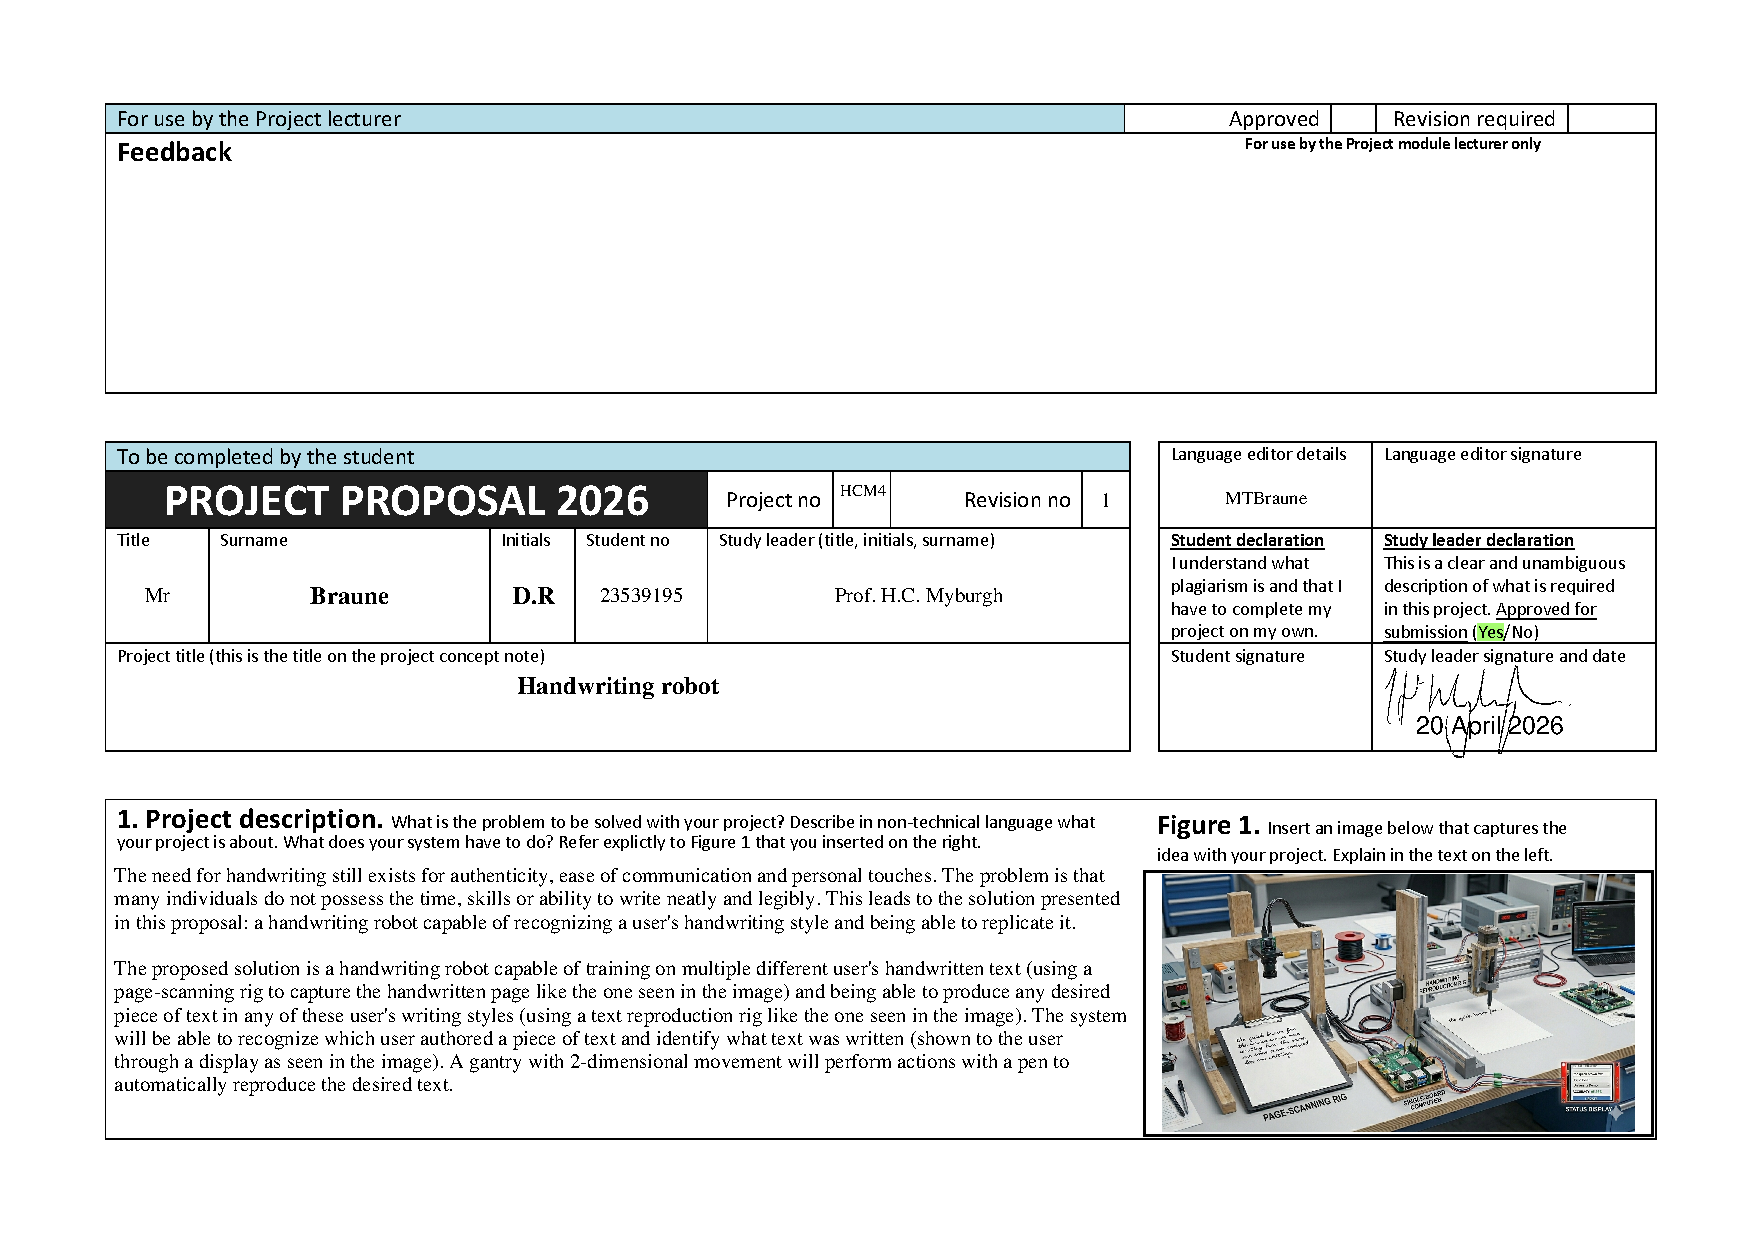
\includepdf[pages=-,landscape]{2_Project_Definition/project_proposal_flat.pdf}


\eprsec{Part 3. Main Report}
\newpage

%% Reset the page number style and count.
\pagenumbering{arabic}
\setcounter{page}{1}

%% The abbreviation and notation lists in the Preamble are set as longtables and
%% silently consumed table numbers 1 and 2, so the first captioned table of the
%% report came out as "Table 3".  Appendix 4 requires figures and tables to be
%% numbered in separate sequences each starting at 1, so both counters are reset
%% here, at page 1 of Part 3.
\setcounter{table}{0}
\setcounter{figure}{0}

%% Import the main report content

\section{Literature study}
\label{sec:literature}
% ---- styles for the literature-study figures ----
\tikzset{
  litbox/.style={draw,rounded corners=2pt,fill=gray!12,align=center,font=\footnotesize,minimum height=7mm,inner sep=3pt},
  litio/.style={draw,rounded corners=6pt,fill=white,align=center,font=\footnotesize,minimum height=7mm,inner sep=3pt},
  litarr/.style={-{Stealth[length=2.0mm]},thick},
  litlab/.style={font=\scriptsize,inner sep=1.5pt,align=center}
}

\new{Text in red is not the author's own wording: it marks the pen-mapping description, the intended contribution, and the individual sentences that were corrected for factual accuracy. All remaining text is the author's own.}

\subsection{Existing concepts}
\label{sec:lit-background}

\subsubsection{A need exists to be able to decode the writer's style and written text from an image}
\label{sec:lit-hwr}

The ability of a computer or system to identify written text after being trained on large amounts of data is known as HWR (Handwriting Recognition) or HTR (Handwritten Text Recognition)~\cite[p.~39]{chen2023}.
One type of handwritten text recognition is offline recognition, which means the data being identified by the system is static and captured post-completion of the page of handwritten text. This is ideal for identifying the text from a fixed image of handwritten content by utilizing image processing techniques and algorithms to identify the text that was written~\cite{ma2023}. The other type is online recognition, which is a more dynamic process that identifies text during the creation of the handwriting, adding the variable of time to the classification of text. The addition of a time variable includes data about the order of strokes to create text as well as pen-up or pen-down movements, which can influence the type and ability of reproduction and handwriting synthesis methods.

Every stage of the process to achieve accurate handwritten text recognition requires a deep understanding of the different techniques available:

\textbf{Datasets and resolution:} Multiple datasets have typically been used for training handwritten text recognition modules, for example, the EMNIST, MNIST and IAM datasets~\cite[p.~2]{mamun2024}. The EMNIST (Extended Modified National Institute of Standards and Technology) dataset consists of approximately 814\,255 handwritten characters and numbers, each being 28 by 28 pixels in size~\cite[p.~40]{chen2023}. There is only a single, disconnected character per image, which is used in many existing HTR models, but these models cannot effectively decipher connected handwritten words, like cursive words. The IAM handwriting dataset provides much more variety, as it consists of 5\,685 complete sentences, with a total of 115\,320 words, gathered from 657 different authors, consisting of 26 letters and 27 punctuation marks~\cite{iamdb}; the paper that introduced the database reports an earlier state of it, 1\,066 forms by about 400 writers~\cite[p.~39]{marti2002}. The images from the IAM dataset were scanned at 300 dpi with 8 bits per pixel in grayscale~\cite{iamdb}. The dataset used influences the accuracy for the classification of text with higher variation, as well as defines the resolution of the camera required to capture the handwritten text to classify. \new{The IAM distribution of cropped lines is not organised by author, so the writer is not evident from the line images alone, while the distribution of full pages is arranged so that each page belongs to a known writer; the database does record the writer of every form in its metadata, so the two can be joined~\cite{marti2002}.}

\textbf{Image-conditioning:} The image-conditioning of handwriting pages includes multiple techniques to be performed on the handwritten text before being passed into the classification and feature recognition algorithms. This is used to account for dimensional adjustments, removal of inconsistencies, and normalization of the data, to make the images more appropriate for text separation and classification~\cite{hemanth2022}. Normalization is used to increase the accuracy of HTR models by reducing the effect that unwanted features of the data could have on the performance of the model. There are multiple different normalization techniques such as min-max scaling, z-score normalization, and log-scaling. Encoding techniques are also used in HTR model pre-processing to get rid of unintentional biases~\cite[pp.~40--41]{chen2023}. Binarization is used to differentiate the background page and obscurities from the actual ink of the written text, computed by pixel. One method of binarization is done from a global ink threshold taken from the grey-level histogram, which does not require any parameters like a localized shadow level radius, and is used for ideal, evenly lit page scans. The other method involves a localized threshold computed per pixel out of the statistics of a window around it, which costs more in terms of computation time and power but can tolerate a lighting gradient or shadow. Deskewing is a technique used to fix the rotation of scanned pages, by rotating the page through certain angle steps until the horizontal projection of the ink is most sharply peaked, which occurs when the lines of text all mostly lie horizontally. Deslanting is used to fix the lean of the individual characters \new{by applying a horizontal shear that shifts each row sideways in proportion to its height}, forcing more pixels to be aligned within the same column rather than slanted over multiple columns.

\textbf{Text Separation:} Text separation is the process of breaking up a page of handwritten text into smaller segments or blocks that can be used in feature extraction and neural network classifiers. There are three methods that existing models employ to separate text: line separation, individual character separation or word separation. All three methods involve breaking down paragraphs of handwritten text into smaller segments. The accuracy of the extraction of smaller segments heavily influences the effectiveness of the classifier. Some existing techniques for this are classic dissection techniques, recognition-based segmentation, hysteresis thresholding, and bounding box techniques~\cite[p.~41]{chen2023}. Line separation can be done by converting images to grayscale, obtaining inverted binary images, and then drawing bounding boxes over each line~\cite{hemanth2022}. Firstly, when lines are mostly straight and separated by a blank row, line separation can be performed by reading the minimums of the row ink profile (the sum of ink in each row) to form boundaries. When descenders of lines begin to overlap or merge, the straight row boundary separator is replaced with a boundary that bends around the descenders by performing a least-cost path traced between the ink lines, and around the descenders.
To achieve either word or character separation, the page must still be broken up into individual lines and then into separate words. Character separation just goes one step further and splits the word into individual characters.

\textbf{Types of Neural Networks:} Many different types of neural network models have been implemented in previous papers, including ANNs (artificial neural networks), CNNs (convolutional neural networks), RNNs (recurrent neural networks), and various combinations of them to achieve the best accuracy.

ANNs are created from the standard neural network architecture consisting of multiple neurons, weights, hidden layers, biases, etc., and can accurately perform pattern recognition for handwritten text. CNNs are built on the architecture of ANNs but also facilitate feature extraction and identifying smaller, more important information in text. This leads to a reduction of necessary learnable parameters and streamlines model training~\cite{ma2023}. RNNs contain the same fundamental structure as CNNs but also have the capability to consider sequential and dependent data. The ability to capture time-dependent patterns is useful for deciphering various handwritten fonts, and because RNNs can consider dependencies in the data, this can improve the accuracy of handwritten text recognition when considering common linguistic dependencies in language~\cite{ma2023}.
A combination of both CNNs and RNNs can significantly enhance feature extraction by using the CNN's pattern recognition and ability to identify diverse handwriting styles, and the RNN's ability to use textual dependencies for improved contextual understanding~\cite{kumar2024}. This combination for improved context awareness allows an entire line of text to be read without word or character separation. The convolutional layers are used to convert a cropped line of text into different feature columns, and the bidirectional recurrent layer reads the sequence of features in each direction, providing context of what comes before and after each character or feature. This implementation is used for unconstrained offline handwriting~\cite[p.~855]{graves2009}, \new{meaning natural handwriting that is not restricted to isolated characters or to a fixed vocabulary, and the full line crop must exist before classification can begin because the recurrent layer reads it from both ends}. In an RNN, the gradient is multiplied by the same weight matrix at every time step as it propagates backwards, so over many steps it shrinks and loses its effect (this is the vanishing gradient problem). Forget gates are added to bypass the vanishing effect and allow gradient errors to still retain an effect after many time steps. Putting convolutional layers before the recurrent stack allows the feature extraction and sequence reading to be trained as one network~\cite{shi2017}. The columns produced from the convolutional layers and max pooling tend to outnumber the number of characters to be classified, therefore \new{the CTC (connectionist temporal classification) loss~\cite[p.~370]{graves2006} is used, which adds a blank symbol and sums the probability of every column-to-character alignment that collapses to the transcription, the collapse being to squash repeated symbols first and then remove the blanks}. The arrangement is shown in Figure~\ref{fig:lit-line}.

\begin{figure}[!htbp]
\centering
\begin{tikzpicture}[x=1cm,y=1cm,font=\footnotesize,node distance=4.5mm]
\node[litio,text width=1.5cm] (img) {line image};
\node[litbox,right=of img,text width=1.7cm] (cnn) {convolutional\\layers};
\node[litbox,right=of cnn,text width=1.6cm] (cols) {$T$ feature\\columns};
\node[litbox,right=of cols,text width=1.9cm] (rnn) {recurrent layer,\\both directions};
\node[litbox,right=of rnn,text width=1.6cm] (pc) {symbol per\\column};
\node[litio,right=of pc,text width=1.1cm] (out) {\texttt{the}};
\foreach \a/\b in {img/cnn,cnn/cols,cols/rnn,rnn/pc,pc/out}{\draw[litarr] (\a) -- (\b);}
%% the two reading directions
\draw[litarr] ([yshift=3.2mm]rnn.north west) -- ([yshift=3.2mm]rnn.north east);
\draw[litarr] ([yshift=6.0mm]rnn.north east) -- ([yshift=6.0mm]rnn.north west);
%% the blank-augmented output and the collapse
\node[litlab,below=2.0mm of pc,font=\ttfamily\scriptsize] (sym) {-tt-h-ee};
\node[litlab,below=1.6mm of sym] {collapse repeats,\\drop the blanks};
\node[litlab,below=2.0mm of cols,text width=2.5cm] {$T$ far exceeds the\\number of characters,\\so the alignment is\\not known};
\end{tikzpicture}
\caption{Reading a whole text line without cutting out characters, after the arrangement of Kizilirmak and Yanikoglu~\cite[pp.~4--5]{kizilirmak2023}. The convolutional layers produce $T$ feature columns, a recurrent layer reads them in both directions, and a symbol including a blank is emitted per column; collapsing repeats and removing the blanks gives the transcription.}
\label{fig:lit-line}
\end{figure}

\textbf{Existing Models:} Two baseline models have been primarily considered in existing research papers: the LeNet-5 CNN model and the ResNet-34 CNN model. LeNet-5 is the most common of the two and was created by Yann LeCun in \new{1998}~\cite[Fig.~2]{lecun1998}. It is a CNN structure that consists of \new{seven} layers, including 3 convolutional layers, 2 pooling layers, and lastly, 2 fully connected layers. A fully connected layer refers to a portion of a typical ANN model, while the convolutional layers and pooling layers will be discussed later in this literature study. The input size to the model is 32 by 32 pixels, and the model uses a hyperbolic tangent activation function in the fully connected layers and a softmax activation function in the output layer. This model is popular for use in object detection and image classification~\cite{chen2023}.
ResNet-34 is also a popular CNN model known for its residual architecture. \new{The residual architecture adds skip connections that let the gradient bypass layers, which is what allows the network to be trained at that depth; separately, its weights from training on a large image set are commonly reused by transfer learning, which forms the foundation of the feature extraction in this model and allows for fast and efficient training from limited datasets}~\cite{ma2023}.

\textbf{Feature extraction:} The convolutional layers of a CNN are used to perform feature extraction, which means they can capture subtle patterns in different areas of a segment of text by sliding a convolutional kernel over the character or word image. Translation invariance is created by sliding the convolution kernel, which allows consistent patterns to be extracted from images~\cite{ma2023}. An $N$ by $N$ input layer is convolved with an $f$ by $f$ kernel and returns an $(N-f+1)$ by $(N-f+1)$ output. Feature maps are created by applying convolutions to different sections of the image being classified. By identifying common features, the kernel-sliding convolutional technique can produce more accurate classification. Each extracted feature is multiplied with a corresponding kernel value to produce a weighting, and then a bias and activation function are applied until an output feature map is obtained~\cite{yahya2021}.

An extended version of the standard CNN is the deep CNN, which refers to a CNN that can extract higher-complexity features like handwritten strokes. The problem is that a larger, deeper CNN creates a `vanishing gradient' problem where there are so many layers that during backpropagation, some layers never get their weightings changed. Thus, there is a limit to the number of layers a standard CNN can have, where adding more layers yields no further benefit. This is why a residual network is used to implement a deep CNN by using residual blocks and skip connections across various layers so that all layers will still update their weightings during backpropagation regardless of the number of layers~\cite{ma2023}.

After a singular round of feature selection, many parameters are still required to classify text with these high-level features. Max-pooling is used to downsample these feature maps until only the essential features remain, minimizing the number of parameters needed to classify handwritten characters and preventing overfitting~\cite{ji2021}. Figure~\ref{fig:lit-conv} shows one convolutional layer followed by one max-pooling layer, which is the unit the models are stacked from.

\begin{figure}[!htbp]
\centering
\begin{tikzpicture}[x=1cm,y=1cm,font=\footnotesize]
%% input N x N with the f x f kernel window
\draw[step=0.26,gray!50,thin] (0,0) grid (1.56,1.56);
\draw[thick] (0,0) rectangle (1.56,1.56);
\fill[gray!40,opacity=0.75] (0.26,1.04) rectangle (1.04,1.56);
\draw[very thick] (0.26,1.04) rectangle (1.04,1.56);
\node[litlab,below] at (0.78,-0.10) {input, $N\times N$};
\node[litlab,above] at (0.78,1.62) {$f\times f$ kernel slides};
%% arrow 1
\draw[litarr] (1.75,0.78) -- (2.60,0.78);
\node[litlab,above] at (2.17,0.86) {multiply,};
\node[litlab,below] at (2.17,0.72) {add bias};
%% feature map (N-f+1)
\draw[step=0.26,gray!50,thin] (2.80,0.13) grid (3.84,1.43);
\draw[thick] (2.80,0.13) rectangle (3.84,1.43);
\fill[gray!40,opacity=0.75] (2.80,1.17) rectangle (3.06,1.43);
\node[litlab,below] at (3.32,0.03) {feature map,};
\node[litlab,below] at (3.32,-0.22) {$(N-f+1)\times(N-f+1)$};
\node[litlab,above] at (3.32,1.49) {activation applied};
%% arrow 2
\draw[litarr] (4.03,0.78) -- (4.88,0.78);
\node[litlab,above] at (4.45,0.86) {max-pool};
\node[litlab,below] at (4.45,0.72) {$2\times2$};
%% pooled map
\draw[step=0.26,gray!50,thin] (5.08,0.39) grid (5.60,1.17);
\draw[thick] (5.08,0.39) rectangle (5.60,1.17);
\node[litlab,below] at (5.34,0.29) {downsampled};
\node[litlab,below] at (5.34,0.04) {feature map};
%% stacking note
\draw[litarr,dashed] (5.79,0.78) -- (6.55,0.78);
\node[litlab,right,align=left] at (6.60,0.78) {repeated, each stage\\ holding more feature\\ maps than the last};
\end{tikzpicture}
\caption{One convolutional layer and one max-pooling layer. The kernel slides over every position of the input, so an $N\times N$ input gives an $(N-f+1)\times(N-f+1)$ feature map, which pooling then downsamples.}
\label{fig:lit-conv}
\end{figure}

\textbf{Training:} The way networks are trained corresponds to the architecture they are built from. The weights are initially randomized with a variance determined by the size of each layer so the signal remains constant as it passes through more layers~\cite{he2015}. Batch normalization is the process of taking the outputs of the current batch of training data and subtracting the average and dividing by their \new{standard deviation}~\cite[Alg.~1]{ioffe2015}. Having more sensibly ranged values allows a higher learning rate to be used safely. Dropout is a technique used to reduce overfitting which removes a random subset of \new{a layer's outputs on each training step}~\cite[p.~1930]{srivastava2014}. This introduces variation and prevents the network from depending on any single feature. Another method to increase variation is dataset enlargement which includes applying shears, small rotations, slants and random smooth warps etc. to simulate more variation in training text~\cite{simard2003}. Learning rate reduction is a technique that is used to adjust the learning rate over time to allow for large changes initially to speed up training, and fine learning later on to prevent overshooting. Final accuracy can be calculated as the character error rate (which refers to the number of mismatches in characters compared to the ideal result) or the word error rate, which is calculated from word mismatches. This is usually significantly higher than the character error rate as one character mismatch ruins the whole word~\cite[p.~1]{kizilirmak2023}.

\textbf{Techniques for writer identification:} There are multiple approaches to identifying the author of a written piece of text. The first way is through feature extraction, which measures text-independent features like slant, height, stroke width, word and character spacing, and connectivity between characters. The author is determined by finding which writer possesses the feature metrics closest to that of the text measured. Another feature that can be extracted is the \new{distribution of edge directions in the ink, which gives the} `texture' of the written sentence~\cite{bulacu2007}. The other method of writer identification is using a neural network trained off the author's handwriting, which can use a feature extractor used for text recognition~\cite{ma2023} instead of the hardcoded methods and metrics for quantifying features. Much more content and pages are required to train the author classifiers in this case compared to creating specific feature extracting methods.

\subsubsection{A need exists to reproduce text on paper accurately and fast in any writer's style}
\label{sec:lit-synth}

There are various existing text reproduction methods and linear actuation techniques which can influence the accuracy and speed of text reproduction.

\textbf{Handwriting synthesis in a writer's style:} Before being able to reproduce handwriting through hardware, the desired text to be reproduced has to still be created in the particular author's style. \new{Four} methods will be discussed on how to achieve this:

\emph{Recurrent stroke level synthesis:} A recurrent neural network is used to predict not the characters to be written, but rather the pen movement that must be taken next, with small offset predictions at a time~\cite[p.~1]{graves2013}. It creates a spread of possible answers as no letter is written identically. The network is trained off an online recorded sample of someone's handwriting. Since it predicts pen movements the outputs are already presented as movements which a plotter requires. Training a network to produce accurate outputs requires hundreds of lines of online data.

\emph{Adversarial image synthesis:} This method creates an image of text using a GAN (generative adversarial network), which trains a text generator and discriminator to identify fake generated text from real handwritten text~\cite[p.~273]{kang2020}. Both the generator and discriminator improve per round until the generator can produce well-reproduced text and the discriminator can no longer tell the difference. It is called `adversarial' as two networks are trained simultaneously, one to generate text and the other to judge the text. This requires a significant amount of time and compute to train, but the final system produces high quality recognisable text \new{in a single pass once trained}. A text and writer classifier are still required to verify the generated text along the way as well. This method produces a raster image which must be converted to pen paths for a plotter to take.

\emph{Diffusion-based synthesis:} This method generates a fake text raster image by reversing a gradual noise-generating process~\cite[Sec.~1]{dai2024}. The system trains by slowly adding noise to handwritten text, remembering the way noise was added, until the final image is pure random noise. Then to generate a new line of text, the system starts with complete random noise and denoises it until an accurate line of text is reproduced. \new{Only one reference image of the target writer is needed at generation time, although training the model still requires a large set of labelled handwriting images}, yet it requires many steps and time to denoise the random noise image. This method also produces a raster image which must still be converted to pen stroke mappings.

\emph{Glyph-library based synthesis:} This method does not use any generators to create text, but rather assembles words from shapes or glyphs taken out of existing handwritten pages. Haines \emph{et al.}~\cite[p.~26:1]{haines2016} describe a technique that stores a library of labelled glyphs per each user, and then creates the specified sentence by choosing the specific glyphs and then assembling them according to which variant of the glyph the writer usually used in the requested position, and the level of connectedness of the text, the texture of the line of ink, and the spacing of the writing. It requires a small number of handwritten pages per author to create decent glyph libraries, and the main complexities of the method only involve connecting one glyph to another and selecting the most appropriate glyphs.

\textbf{Assessing generated handwritten text:} Accuracy of generated handwriting can be measured through performing image-level distances and correlation to real handwritten text, for example an IoU test (Intersection over Union) which measures the overlap between a predicted region and the true region. Another method is by passing it through an independent text and author classifier and reporting the accuracy of the reproduced text. A survey can also be conducted for human validation of what text appears real and what appears reproduced.

\textbf{Method of reproduction:} There are three main methods to reproduce handwritten text on paper: Cartesian systems, serial-chain robots, and parallel-chain robots. A Cartesian system consists of a gantry with x\,--\,y movement. It has restricted movement in only two directions using linear actuation. Serial-chain robots are the most common in industrial settings for automated movement. They consist of multiple linkages chained together, one component connected to the next in a single chain, like a typical robot arm. The third method is parallel-chain robots, which consist of multiple serial-chain linkages that can precisely control automated movement~\cite{teikari2016}.

\textbf{Pen mapping techniques:} \new{A pen path is stored as a list of points, and a drawn stroke usually has far more points than a plotter needs. Pen mapping is the step that reduces this list while keeping the shape of the stroke. The Douglas-Peucker algorithm is the common choice~\cite{teikari2016}: it draws a straight line between the two ends of a stroke, finds the point that sits furthest from that line, and keeps it only if it is further away than a chosen tolerance, then repeats on each half~\cite{douglas1973}. A small tolerance keeps many points and follows the stroke closely, while a large tolerance keeps few points and cuts corners, so the tolerance sets the trade-off between the file size and the accuracy of the drawn shape. The alternatives are fitting a smooth curve such as a spline through the points, which needs a fit to be solved, and resampling the stroke at a fixed spacing, which spaces the points evenly but ignores where the curves are. When the handwriting only exists as an image, the path has to be recovered first by thinning the ink down to a one-pixel centre line and then joining those pixels into strokes, which means guessing the drawing order wherever two strokes touch or cross.}

\textbf{Linear actuation types:} There are multiple methods of linear actuation that could be considered for a Cartesian plotting system. Some popular examples of linear actuation methods are electric, pneumatic, belt-drive, rack-and-pinion, and ball-screw systems. Electric and pneumatic methods are often used for industrial cases, but belt-drive, rack-and-pinion, and ball-screw linear actuators have been used in multiple handwriting reproduction systems due to their durability, reliability, and cost-effectiveness~\cite{iqs2024}.

\subsection{Intended contribution and discussion}
\label{sec:lit-application}
\label{sec:lit-embedded}

\new{The literature above covers each stage of the problem on its own, but it does not cover them as one machine. Recognition is reported on evenly lit scans or on isolated characters, writer identification is reported over sets of hundreds of writers rather than a small closed group, and handwriting synthesis is judged as an image rather than as something that has to be drawn with one pen. Almost all of this work is also built on libraries such as OpenCV~\cite[p.~41]{chen2023}, which hide what each stage actually costs in operations and memory. That cost matters here, because every stage of this project must run on a single-board computer.}

\new{The main contribution of this project is therefore the full integration of the system, from a photographed page to ink on paper, with every stage implemented from first principles and no machine-learning or image-processing libraries used anywhere in the pipeline. This covers the creation of the dataset, the conditioning and line separation of photographed pages, a line-level text recogniser, the identification of the author, the synthesis of new text in that author's style, and the generation of the pen paths and G-code that drive the gantry. Writing each stage by hand means the forward and backward passes of every layer, the loss functions and the optimisers are known quantities whose cost can be measured and reduced to fit the available hardware.}

\new{Two things set the approach apart from the work reviewed. The first is that the system classifies both the text that was written and the author who wrote it, using the same feature extractor for both, so that one page yields a transcription and an identity. The second is that the synthesised handwriting is produced as geometry rather than as an image, so it can be drawn directly without having to recover a pen path from pixels, and the recogniser and the author classifier are then reused to judge the synthesised output before it is committed to paper. The reasoning behind each of these choices, and the alternatives that were rejected, is given in Section~\ref{sec:design}.}

\newpage

\section{Approach}
\label{sec:approach}
This section explains how the proposal's functional analysis became a first concept, why the subsystems were then built in the order they were, and which alternatives were weighed. Mathematics, component values and experiments belong to Section~\ref{sec:design}.

\subsection{From functional analysis to concept}
\label{sec:app-concept}

The functional analysis describes a chain rather than a collection of parts (Figure~\ref{fig:app-concept}): each block consumes the output of the one before it, so the accuracy of the whole is the product of the accuracies of its parts rather than their average.

The first concept kept the proposal's four functional units, namely page scanning (FU\,1), the single-board computer (SBC) and its eight processing steps (FU\,2), the gantry (FU\,3) and the power supply (FU\,4), and made one decision per block; Table~\ref{tab:des-fumap} in Section~\ref{sec:blockdiagram} maps each unit onto the block that implements it. One decision applies to all of them: no computer-vision or machine-learning library was used, so every block was implemented from first principles with only numpy for array arithmetic. That is why Section~\ref{sec:design} derives methods a library call would hide, and it narrowed the field to those that could be written and verified in the time available.

\begin{figure}[htbp]
\centering
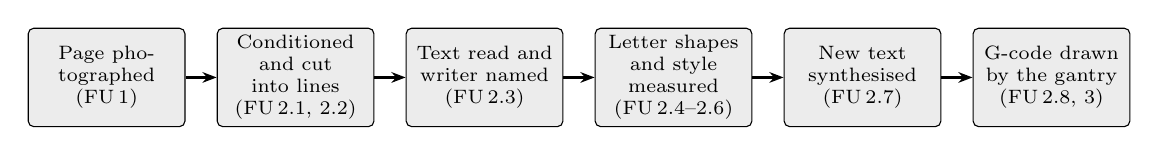
\begin{tikzpicture}[
  blk/.style={draw,rounded corners=2pt,fill=gray!15,minimum height=1.25cm,text width=1.85cm,align=center,font=\scriptsize,inner sep=2pt},
  arr/.style={-{Stealth[length=1.8mm]},thick}]
\node[blk] (a) at (0,0) {Page photographed\\(FU\,1)};
\node[blk] (b) at (2.4,0) {Conditioned and cut into lines\\(FU\,2.1, 2.2)};
\node[blk] (c) at (4.8,0) {Text read and writer named\\(FU\,2.3)};
\node[blk] (d) at (7.2,0) {Letter shapes and style measured\\(FU\,2.4--2.6)};
\node[blk] (e) at (9.6,0) {New text synthesised\\(FU\,2.7)};
\node[blk] (f) at (12,0) {G-code drawn by the gantry\\(FU\,2.8, 3)};
\draw[arr] (a)--(b); \draw[arr] (b)--(c); \draw[arr] (c)--(d);
\draw[arr] (d)--(e); \draw[arr] (e)--(f);
\end{tikzpicture}
\caption{The chosen concept as a chain, with the proposal's functional-unit numbers. Training builds the style store from the first four blocks and runs offline, classification stops after the third, and reproduction runs the last two. The as-built hardware and software block diagrams are Figures~\ref{fig:des-hw} and~\ref{fig:des-sw}.}
\label{fig:app-concept}
\end{figure}

Seven departures from that concept are declared with their reasons in Table~\ref{tab:des-fumap}; the three that shaped it are the separation of text lines rather than characters, since joined letters have no reliable boundaries, the split of FU\,2.3 into two networks instead of one character classifier, and training off the SBC, which needs far more memory than inference, with all inference left on the SBC as required. \mustdo{state on which computer the networks were trained and the profiles built; the proposal requires embedded-only processing.} \mustdo{reason for the pen-lift change.} \mustdo{supply voltages, current ratings and distribution for FU\,4.}

\subsection{Order in which the subsystems were built}
\label{sec:app-order}

Figure~\ref{fig:app-concept} is a data path, and the subsystems were deliberately not built along it. The design divides into a motion subsystem and a software subsystem meeting at one interface, a file of G-code; fixing it at the outset decoupled them, since the gantry draws any valid G-code whatever produced it. The gantry was therefore built first and on its own (Section~\ref{sec:gantry}): the 0.5\,mm limit of R5 is set by its mechanics, transmission and step resolution alone, so nothing in it depends on which recogniser or synthesis route was later chosen, and it carries the only schedule risk outside the work itself, since parts take time to arrive and may arrive faulty. Hand-written G-code was enough to commission and measure it before any software existed.

The software allowed no such freedom, because an error in one block propagates and compounds and is hardest to see at its origin: a slightly mis-cut text line is still a plausible image while it silently bounds the accuracy of everything downstream. Each block was therefore brought to a measured standard before the next was begun, in pipeline order --- conditioning and line segmentation (Section~\ref{sec:segmentation}), without whose clean labelled line images no network can be trained; the recogniser and then the writer classifier (Sections~\ref{sec:textrec} and~\ref{sec:writerid}), in that order because the second reuses the first's feature extractor; glyph and style extraction (Section~\ref{sec:styleprofile}), which needs the recogniser to locate the letter shapes; synthesis (Section~\ref{sec:synthesis}); and G-code generation (Section~\ref{sec:gcode}). The page-scanning rig was fixed during the first of these, once freehand photographs rather than the algorithm proved to be what limited the result, since a camera held at one height looking straight down removes scale, tilt and framing variation at source; a flatbed scanner would have lit it more evenly but is larger and slower.

\subsection{Design alternatives and trade-offs}
\label{sec:app-alternatives}

Each decision was weighed against the same criteria: accuracy (R1, R2), processing time on the SBC (R3, R4), the data available for thirteen writers (R6), implementation from first principles, and mechanical and electrical simplicity and safety. Table~\ref{tab:app-tradeoffs} gives the alternatives and the reason for each preference.

\begin{table}[htbp]
\centering
\fontsize{8}{9.4}\selectfont
\begin{tabular}{|p{2.5cm}|p{6.6cm}|p{4.2cm}|}
\hline
\textbf{Decision} & \textbf{Alternatives considered and how they compare} & \textbf{Preferred and reason} \\
\hline
\multicolumn{3}{|l|}{\textbf{Hardware}} \\
\hline
Robot type & (a) Cartesian gantry: identity kinematics, axis errors do not add up. (b) Serial arm: inverse kinematics, joint errors add up. (c) Parallel robot: stiff, but a small workspace and complex kinematics. & (a): position follows from step counts, so the 0.5\,mm limit of R5 is simplest to meet and verify~\cite{teikari2016}. \\
\hline
Interface to the gantry & (a) A custom protocol fits the synthesiser exactly, but only the synthesiser can then exercise the machine. (b) G-code is a standard shared with commercial equipment, readable and writable by hand. & (b): it let the gantry be commissioned and measured before any software block existed, and keeps the two subsystems independently testable. \\
\hline
\multicolumn{3}{|l|}{\textbf{Software}} \\
\hline
Unit of recognition & (a) Cut characters and classify each: needs character-level labels, which are absent, and cannot repair a wrong cut. (b) Cut lines and read with a sequence recogniser: no boundaries below the line, context used, larger network. & (b): cursive cannot be segmented reliably, labels exist per line, and segmenter errors would bound system accuracy. \\
\hline
Synthesis of writing & (a) A neural generator needs recorded pen trajectories, which are unavailable. (b) Pretrained image generators give raster output, no control of size or slant, and are slow without a graphics processor. (c) A library of the writer's own letter shapes needs only nine pages and gives controllable strokes, but loses some cursive links. & (c): a from-scratch generator learned slant and roundness but not legible letters, and image generators took tens of seconds per line on a processor-only computer. \\
\hline
\end{tabular}
\caption{Design decisions, alternatives considered and the reason for each preferred solution.}
\label{tab:app-tradeoffs}
\end{table}

Each block was held to a measurable criterion from the requirements --- characters read correctly, writers named, lines cut correctly, pen position in millimetres --- and measured alone before the chain was measured end to end; where no known truth exists, as for the drawn page, a round trip was used. That measurement later replaced four designs, collected in Section~\ref{sec:later}. Only the camera, SBC, motors, drivers, switches, pen, standard gantry parts and power supply were bought. \mustdo{list the mechanical parts I designed and made.} Section~\ref{sec:design} takes each block in build order, so each is met with its input explained.

\newpage

\section{Design and implementation}
\label{sec:design}

%% Order of the subsections, v5 restructuring (component-based design).
%% Each of the four main subsections (3.3-3.6) is organised by COMPONENT
%% rather than by phase: every component subsubsection carries its own
%% theory, formulas, design calculations, design description and tests
%% together, per the component-subsubsection structure requested for v5.
%%   3.1, 3.2  the compulsory summary and system block diagram
%%   3.3       hardware: drive train, driver/pen circuits, resolution and
%%             calibration, end-stops and pen mechanism, G-code and motion
%%   3.4       page conditioning and line segmentation
%%   3.5       text recognition and writer identification (shared backbone)
%%   3.6       style extraction, glyph library and handwriting synthesis
%%   3.7       design reconsiderations: four changes made once the whole
%%             chain could be measured, plus one identified but not yet made
%%   3.8       integration of all of the above on the single-board computer
%% Every cross-reference uses \ref, so the numbering follows this order
%% automatically and the files may be reordered again without further edits.

% ---- Writer 2 shared definitions (used by 3.1 - 3.5) ----
\providecommand{\wht}{h_{\mathrm{t}}}
\tikzset{
  w2box/.style={draw,rounded corners=2pt,fill=gray!12,align=center,font=\footnotesize,minimum height=7mm,inner sep=3pt},
  w2dark/.style={draw,rounded corners=2pt,fill=gray!30,align=center,font=\footnotesize,minimum height=7mm,inner sep=3pt},
  w2store/.style={draw,fill=white,align=center,font=\footnotesize,minimum height=7mm,inner sep=3pt,double,double distance=1pt},
  w2io/.style={draw,rounded corners=6pt,fill=white,align=center,font=\footnotesize,minimum height=7mm,inner sep=3pt},
  w2arr/.style={-{Stealth[length=2.2mm]},thick},
  w2dash/.style={-{Stealth[length=2.2mm]},thick,dashed},
  w2group/.style={draw,dashed,rounded corners=4pt,inner sep=5pt},
  w2lab/.style={font=\scriptsize,inner sep=1.5pt}
}

\subsection{Design summary}
\label{sec:summary}

This section summarises the project design tasks and how they were implemented (see Tables~\ref{tab:des-summary} and~\ref{tab:des-summary2}).
The rows are the deliverables of line~5 of the table in Section~4 of the approved project proposal and the nine tasks of its Section~6.1.
The summary is split over two tables only so that neither runs across a page break; the headings are the same in both.
A task is marked \emph{Completed} only when the deliverable itself works. Where any part of it is missing, unbuilt or unmeasured it is marked \emph{Incomplete}, and the second column says what is missing.
Only work designed and implemented by the student is claimed. The parts that were bought as finished items, namely the camera, the single-board computer, the motors and their driver modules, the pen, the switches, the power supply and the standard mechanical parts, carry no design credit.
Every image-processing, machine-learning, trajectory and motion-control algorithm in the running system was written by the student in Python on top of NumPy array arithmetic. No machine-learning framework supplies any layer, gradient or optimiser. The exceptions are all on the offline training path or at the interfaces, and are listed in declaration~6 of the preamble. SciPy is used in exactly two files, for peak finding when the public database pages are cut into lines and for the Gaussian filtering and coordinate mapping of the elastic augmentation; the remaining libraries interface with the camera, the general-purpose pins, the image files, the database download and the network.

Two deviations from the proposal shape several rows.
First, the proposal planned to separate the page into characters (functional unit 2.2) before classification. The implemented design separates the page into text lines only and reads each line with a sequence recogniser, because the characters of joined handwriting have no reliable boundaries and a separation error would pass straight into a wrong reading (Sections~\ref{sec:segmentation} and~\ref{sec:textrec}).
Second, the proposal placed training and the building of trajectory maps on the single-board computer (functional units 2.4 to 2.6). In the implemented system the networks and the per-writer style profiles are produced by offline programs on a general-purpose computer, and only inference, synthesis and motion control run on the board. The interface therefore offers no training mode.
\mustdo{state the computer used for network training (the project notes mention a laptop processor and a cloud notebook) and confirm that the single-board computer was not used for training.}

\begin{table}[!htbp]
\centering
\fontsize{8}{9.4}\selectfont
\setlength{\tabcolsep}{3pt}
\renewcommand{\arraystretch}{1.0}
\begin{tabular}{|p{3.1cm}|p{7.4cm}|p{3.7cm}|}
\hline
\textbf{Deliverable or task} & \textbf{Implementation} & \textbf{Completion of deliverable or task, and section in the report} \\
\hline
Research of network types, structure, layers and feature extraction (task 6.1.1) &
A literature study of convolutional, recurrent and sequence-to-sequence recognisers, of writer-identification methods and of the alternatives to each, used to choose the methods of Sections~\ref{sec:textrec} and~\ref{sec:writerid}. &
Completed. Section~\ref{sec:literature}. \\
\hline
Research of conditioning, noise removal, separation and trajectory mapping (task 6.1.2) &
A literature study of thresholding, illumination correction, line and character separation, thinning and exemplar-based handwriting synthesis, used to choose the methods of Sections~\ref{sec:segmentation} and~\ref{sec:styleprofile}. &
Completed. Section~\ref{sec:literature}. \\
\hline
Image conditioning and noise removal (FU 2.1; R2, R4) &
Implemented from first principles using only array arithmetic: size normalisation, page localisation, flat-field illumination correction with summed-area tables, local adaptive thresholding, skew correction and removal of printed rules, faint print and neighbouring-page ink. The individual operations are standard and are cited in Section~\ref{sec:segmentation}; the stages chosen, their order and every threshold were settled for this project. &
Completed. Section~\ref{sec:segmentation}. \\
\hline
Separation into characters (FU 2.2; R2, R4) &
Implemented as separation into text lines and diagram regions rather than into characters (connected components, glyph-scale estimation, chaining, baseline merging, text versus non-text scoring, one deskewed crop per line). Character territories are derived only offline, by forced alignment, when style profiles are built. The reason for the change from the proposal is given above and in Section~\ref{sec:textrec}. &
Completed. Sections~\ref{sec:segmentation}, \ref{sec:textrec}. \\
\hline
Optimised and efficient character separation (R4; task 6.1.3) &
The segmentation was profiled and its two dominant routines, component labelling and the box sums, were rewritten in C by the student at 84 to 88\% faster each, 25 to 32\% faster per page. The C routines are not called by the deployed program, and segmentation still exceeds the R4 allowance by over an order of magnitude. &
Incomplete. Sections~\ref{sec:segmentation}, \ref{sec:results}. \\
\hline
Neural network that decodes the text (FU 2.3; R2) &
Convolutional and bidirectional recurrent network with connectionist temporal classification (CTC) output, 3\,358\,763 trainable parameters. The layer pattern follows a published design~\cite[p.~9]{kizilirmak2023}; the student chose the input geometry, data pipeline, label cleaning, augmentation and staged training, and wrote the from-scratch module (forward and backward passes, optimisers, no machine-learning library) used by training, validation and deployment alike. &
Completed. Section~\ref{sec:textrec}; measured accuracy 98.61\% character and 94.21\% word on 669 real line crops (Section~\ref{sec:results}). \\
\hline
Neural network that identifies the writer (FU 2.3; R2) &
Two thirteen-class convolutional classifiers sharing the recogniser's backbone and layer module: an ink-based one for photographs, which reached 99.78\% over 1358 real lines, and one whose input is re-drawn at a constant pen width by the student's stroke normalisation, with page-level aggregation. &
Completed. Section~\ref{sec:writerid}; measured accuracy 93.67\% for the normalised classifier after a training fault was corrected (Section~\ref{sec:results}). \\
\hline
Training on datasets and choice of layer numbers (FU 2.4; task 6.1.4) &
Training programs for the recogniser and both classifiers on a public database, a public line-level set and the photographed personal pages, all built on the from-scratch module of Section~\ref{sec:textrec-numpynn}, whose every layer gradient was checked against numerical differentiation in 78 configurations. A sweep over widths, depths and learning rates was programmed but no result was kept, so the layer numbers are the published design's and are not justified by this project's own measurement. Training is offline. &
Incomplete. Sections~\ref{sec:textrec}, \ref{sec:writerid}. \\
\hline
Trajectory maps and permanent storage (FU 2.5 to 2.7; R1, R6) &
Letter shapes are harvested by forced alignment with the recogniser, thinned to centre-line pen paths, normalised and stored as one JavaScript Object Notation (JSON) file per writer with measured style statistics; thirteen styles exist, for eight database writers and five personal writers. The builder is an offline program. &
Completed. Section~\ref{sec:styleprofile}. \\
\hline
Pen trajectory mapping and G-code (FU 2.5 to 2.8; R1, R3) &
A synthesiser assembles the writer's own letter paths into lines (slant, spacing, joins, wobble) with a best-of-$N$ search judged by the recogniser and the writer classifier; a generator turns the trajectory into G-code, the numerical-control command language of plotters, with placement, stroke ordering and pen-state tracking, and a simulator replays it. &
Completed. Sections~\ref{sec:synthesis}, \ref{sec:gcode}. \\
\hline
Optimisation of pen movement (R3) &
Greedy nearest-endpoint stroke ordering reduces pen-up travel. The saving it achieves was not measured. &
Completed. Section~\ref{sec:gcode}. \\
\hline
\end{tabular}
\caption{Design summary, part 1 of 2: the research, image-processing, network and trajectory tasks.}
\label{tab:des-summary}
\end{table}

\begin{table}[!htbp]
\centering
\fontsize{8}{9.4}\selectfont
\setlength{\tabcolsep}{3pt}
\renewcommand{\arraystretch}{1.0}
\begin{tabular}{|p{3.1cm}|p{7.4cm}|p{3.7cm}|}
\hline
\textbf{Deliverable or task} & \textbf{Implementation} & \textbf{Completion of deliverable or task, and section in the report} \\
\hline
Capture rig and deployment on the single-board computer (FU 1; R2, R4; task 6.1.5) &
A generic USB camera in a printed housing that clamps the page flat, read with a live preview and a five-frame warm-up; the recognition, synthesis and motion programs run on the ODROID N2+ behind a web server. The rig geometry, camera resolution and lighting are not documented. \mustdo{camera model, resolution, mounting height, field of view, lamp, lux readings, photograph of the rig.} &
Incomplete. Sections~\ref{sec:blockdiagram}, \ref{sec:system}. \\
\hline
Testing the classifier on the single-board computer with captured images (task 6.1.6) &
The deployed programs were written to run on the board and do run on it, but no accuracy or timing figure in this report was obtained on the board; every measurement reported in Section~\ref{sec:results} was taken on a laptop. &
Incomplete. Section~\ref{sec:results}. \\
\hline
Gantry design and construction in CAD (FU 3.3, 3.4; R5; task 6.1.7) &
A Cartesian X/Y gantry built by the student from bought parts: one motor turning an 8\,mm cross-shaft that drives both ends of the moving bridge, and a second motor on that bridge driving the carriage, both on GT2 belts over linear bearings and chromed rods, with four end-stops. Hand-measured travel 204\,mm (X) and 262\,mm (Y). The machine exists but no CAD drawing or photograph was kept. \mustdo{CAD files and photographs.} &
Incomplete. Section~\ref{sec:gantry}. \\
\hline
Pen holder, pen adjuster and paper holder (R5) &
The pen is carried on the moving carriage in a holder with the toggle cam of the lift mechanism above it, and the page is clamped flat in the camera housing for capture. Whether the holder provides a pen-height adjustment, and how the paper is held on the writing bed, are not recorded. \mustdo{confirm how the pen height is adjusted and how the paper is held down on the writing bed, and supply a photograph of each; neither is documented in the project files.} &
Incomplete. Section~\ref{sec:gantry}. \\
\hline
Power supply (FU 4) &
A 24\,V supply feeds both stepper drivers through a 100\,\textmu F bulk capacitor. The conversion to the voltages the single-board computer and the pen motor require is not documented, no power budget was drawn up and the supply's rating is unknown. &
Incomplete. Section~\ref{sec:gan-supply}. \\
\hline
Stepper-motor control and pen lift (FU 2.8, 3.1 to 3.4; R5; task 6.1.8) &
A G-code interpreter generates step and direction pulses directly on the general-purpose pins, with Bresenham interpolation, absolute step bookkeeping, calibration between end-stops, debounced end-stop monitoring and software limits. The pen is lifted by a toggle gear motor confirmed by a position switch, switched by a transistor stage designed by the student, rather than through the stepper driver as the proposal planned. During bring-up the X-axis direction pin was not observed to change level on reversal and that fault was not resolved. &
Incomplete. Section~\ref{sec:gantry}. \\
\hline
Smooth motor control for efficient gantry movement (R3) &
The interpreter steps at a constant interval within a segment and executes no acceleration ramp, although the generator's time model assumes one. Abrupt starts at the feeds used may lose steps, and no torque margin was computed because the carriage masses were not measured. &
Incomplete. Sections~\ref{sec:gan-mech}, \ref{sec:gan-res}. \\
\hline
Display and user interface (R4, R6) &
A web server exposes classification, generation, calibration and sending of jobs; browser pages show the text, the writer with a confidence, the stored writers and a G-code preview. The synthesis time is returned, but the classification time that R4 asks to be displayed is not shown. &
Incomplete. Section~\ref{sec:system}. \\
\hline
Full-system testing against the requirements (task 6.1.9) &
The accuracy, writer-identification and timing evaluations of Section~\ref{sec:results} were designed and run by the student. The physical writing time of R3, the on-board timing of R4, the positional error of R5 and the random-writer reproduction of R6 were not measured, because the gantry bring-up was not completed. &
Incomplete. Section~\ref{sec:results}. \\
\hline
\end{tabular}
\caption{Design summary, part 2 of 2: the capture rig, the gantry hardware, the motion control and the verification tasks.}
\label{tab:des-summary2}
\end{table}


\subsection{System block diagram}
\label{sec:blockdiagram}

Two diagrams describe the implemented design: Figure~\ref{fig:des-hw} gives the hardware blocks and how they connect to the single-board computer, and Figure~\ref{fig:des-sw} gives the software data flow of the three modes of operation, which are reproduction, classification and offline training.
Both follow the functional block diagram of the approved proposal, which divided the system into the page-scanning set-up (FU~1), the single-board computer (FU~2), the gantry (FU~3) and the power supply (FU~4).
The four physical units were kept, but the software units FU~2.1 to FU~2.8 were reorganised; Table~\ref{tab:des-fumap} relates the implemented blocks to the proposed units and gives the reason for every departure.

\begin{figure}[!htbp]
\centering
\begin{tikzpicture}[x=1cm,y=1cm]
% left column: FU1
\node[w2io,text width=3.0cm] (page) at (-5.6,3.6) {A4 page with handwriting};
\node[w2box,text width=2.9cm] (cam) at (-5.6,1.7) {USB camera on page-scanning rig};
\node[font=\scriptsize\bfseries,anchor=south west] at (-7.1,2.45) {FU 1};
\begin{scope}[on background layer]
\node[w2group,fit=(page)(cam),inner sep=6pt] (fu1) {};
\end{scope}
% SBC
\node[w2box,text width=5.0cm,minimum height=0.85cm] (m1) at (0,4.2) {Web server (API, job handling)};
\node[w2box,text width=5.0cm,minimum height=0.85cm] (m2) at (0,3.2) {Page conditioning and line segmentation};
\node[w2box,text width=5.0cm,minimum height=0.85cm] (m3) at (0,2.2) {Text recogniser and writer identification};
\node[w2box,text width=5.0cm,minimum height=0.85cm] (m4) at (0,1.2) {Handwriting synthesis and G-code generation};
\node[w2box,text width=5.0cm,minimum height=0.85cm] (m5) at (0,0.2) {G-code interpreter and general-purpose pin pulse generator};
\node[w2store,text width=5.0cm,minimum height=0.85cm] (st) at (0,-0.9) {Stored: network weights, ten style profiles};
\begin{scope}[on background layer]
\node[w2group,fit=(m1)(m5)(st),inner sep=7pt] (sbc) {};
\end{scope}
% right column: FU3
\node[w2box,text width=3.1cm] (drv) at (5.6,3.9) {Stepper driver modules for X and Y (STEP/DIR)};
\node[w2box,text width=3.1cm] (mot) at (5.6,2.5) {Stepper motors X and Y};
\node[w2box,text width=3.1cm] (gan) at (5.6,1.3) {X/Y gantry, pen holder and pen};
\node[w2box,text width=3.1cm] (pen) at (5.6,0.1) {Pen-lift toggle gear motor and pen-position switch};
\node[w2box,text width=3.1cm] (end) at (5.6,-1.1) {Four end-stop switches};
\begin{scope}[on background layer]
\node[w2group,fit=(drv)(end),inner sep=6pt] (fu3) {};
\end{scope}
\node[font=\scriptsize\bfseries,anchor=south east] at (7.2,4.55) {FU 3};
\node[font=\scriptsize\bfseries,anchor=south west,align=left] at (sbc.north west) {ODROID N2+ single-board\\ computer (FU 2)};
% laptop
\node[w2io,text width=4.6cm] (lap) at (1.6,6.5) {User's laptop: web browser (input and display)};
% power
\node[w2dark,text width=6cm] (psu) at (0,-2.6) {Power supply (FU 4)};
% arrows
\draw[w2arr] (page) -- (cam);
\draw[w2arr] (cam.east) -- ++(0.55,0) |- (m2.west);
\draw[w2arr,<->] (1.6,6.1) -- (1.6,4.65);
\draw[w2arr] (2.5,0.4) -- (3.8,0.4) |- (drv.west);
\draw[w2arr] (drv) -- (mot);
\draw[w2arr] (mot) -- (gan);
\draw[w2arr,<->] (2.5,0.2) -- (3.5,0.2) |- (pen.west);
\draw[w2arr] (end.west) -| (3.2,0.0) -- (2.5,0.0);
% power (dashed)
\draw[w2dash] (psu.north) -- (sbc.south);
\draw[w2dash] (psu.west) -| (cam.south);
\draw[w2dash] (psu.east) -| (fu3.south);
\node[w2lab,fill=white] at (-3.6,-2.6) {power};
\node[w2lab,fill=white] at (3.6,-2.6) {power};
\end{tikzpicture}
\caption{Hardware block diagram of the implemented system. Solid arrows show signals and data, dashed arrows show the power supply. FU numbers refer to the functional units of the project proposal.}
\label{fig:des-hw}
\end{figure}

\subsubsection{Hardware block diagram}

The hardware of Figure~\ref{fig:des-hw} is four groups. The page-scanning rig (FU~1) holds a generic USB camera above an A4 page, read through the operating system's own driver, so no camera driver was designed by the student. The single-board computer (FU~2) is an ODROID N2+ and runs every software block, including the web server through which a laptop controls the robot. The gantry (FU~3) moves each axis with one stepper motor and one driver module, whose STEP and DIR inputs go straight to general-purpose pins, so there is no separate microcontroller; four end-stop switches bound the travel, and a toggle gear motor with a position switch raises and lowers the pen. The power supply (FU~4) feeds all three.
The circuit itself, with its component values and design calculations, is given in Section~\ref{sec:gantry}.
\mustdo{model numbers of the camera, stepper motors and driver modules, the supply voltages and current ratings of the power supply, the way in which the pen motor is switched, and the logic-level and grounding arrangement between the single-board computer and the drivers; these are not documented in the project files.}

\begin{figure}[!htbp]
\centering
\begin{tikzpicture}[x=1cm,y=1cm]
\tikzset{cb/.style={w2box,text width=2.4cm,minimum height=1.05cm}}
% Row 1 reproduction
\node[font=\scriptsize\bfseries,anchor=west] at (-7.0,5.45) {Reproduction mode (online)};
\node[cb] (r1) at (-5.2,4.6) {Text and writer chosen in browser};
\node[cb] (r2) at (-2.6,4.6) {Style synthesis, best of $N$ candidates};
\node[cb] (r3) at (0,4.6) {Pen trajectory in millimetres};
\node[cb] (r4) at (2.6,4.6) {G-code generator and simulator};
\node[cb] (r5) at (5.2,4.6) {G-code interpreter, step pulses to gantry};
\foreach \a/\b in {r1/r2,r2/r3,r3/r4,r4/r5} \draw[w2arr] (\a) -- (\b);
% stores
\node[w2store,text width=2.4cm] (sw) at (-5.2,2.7) {Network weights};
\node[w2store,text width=2.4cm] (sp) at (5.2,2.7) {Style profiles (one file per writer)};
% Row 3 classification
\node[font=\scriptsize\bfseries,anchor=west] at (-7.0,1.75) {Classification mode (online)};
\node[cb] (c1) at (-5.2,0.8) {Photograph from camera or upload};
\node[cb] (c2) at (-2.6,0.8) {Conditioning and line segmentation};
\node[cb] (c3) at (0,0.8) {One grey crop per text line};
\node[cb] (c4) at (2.6,0.8) {Text recogniser, ink writer classifier};
\node[cb] (c5) at (5.2,0.8) {Text, writer and confidence to browser};
\foreach \a/\b in {c1/c2,c2/c3,c3/c4,c4/c5} \draw[w2arr] (\a) -- (\b);
% Row 4 training
\node[font=\scriptsize\bfseries,anchor=west] at (-7.0,-0.65) {Training mode (offline)};
\node[cb] (t1) at (-5.2,-1.5) {Pages and transcripts};
\node[cb] (t2) at (-2.6,-1.5) {Line segmentation of the photographs};
\node[cb] (t3) at (0,-1.5) {Training of recogniser and writer classifiers};
\node[cb] (t4) at (2.6,-1.5) {Forced alignment and profile builder};
\foreach \a/\b in {t1/t2,t2/t3,t3/t4} \draw[w2arr] (\a) -- (\b);
% store connections (reads, dashed)
\draw[w2dash] (sw.east) -- (-2.6,2.7) -- (r2.south);
\draw[w2dash] (sw.east) -- (2.6,2.7) -- (c4.north);
\draw[w2dash] (sp.west) -- (-2.2,2.55) -- (-2.2,3.97);
% writes (solid) via margins
\draw[w2arr] (t3.south) -- ++(0,-0.55) -| (-6.95,2.7) -- (sw.west);
\draw[w2arr] (t4.south) -- ++(0,-0.55) -| (6.95,2.7) -- (sp.east);
\end{tikzpicture}
\caption{Software data flow of the three modes. Dashed arrows are reads from permanent storage, solid arrows between the training row and the two stores are writes. The same line-segmentation and recognition blocks serve classification, training and the judging of synthesised handwriting.}
\label{fig:des-sw}
\end{figure}

\subsubsection{Software block diagram and systems-level description}

The system learns how a person writes from photographs of that person's pages and later writes new text in the same style.
Figure~\ref{fig:des-sw} shows the three chains of blocks that do this and the two permanent stores they share, the network weights and the per-writer style profiles.
In the classification mode (R2, R4) the page is conditioned and separated into text lines (Section~\ref{sec:segmentation}), each line is read by the text recogniser (Section~\ref{sec:textrec}) and classified by the ink-based writer classifier (Section~\ref{sec:writerid}), and the writer probabilities of the lines are averaged to a page decision.
In the reproduction mode (R1, R3, R5, R6) the synthesiser (Section~\ref{sec:synthesis}) assembles the writer's own stored letter paths (Section~\ref{sec:styleprofile}) into a line, repeats the random construction for $N$ candidates and keeps the one that the recogniser and the stroke-normalised writer classifier jointly prefer; the trajectory is converted to G-code (Section~\ref{sec:gcode}) and executed by the interpreter after the gantry has been calibrated between its end-stops (Section~\ref{sec:gantry}).
The training mode runs offline: the same segmentation block prepares the pages, the networks are trained and the profile builder writes the two stores, after which no image and no training code are needed to use a style.

\begin{table}[!htbp]
\centering
\fontsize{9}{10.8}\selectfont
\begin{tabularx}{\linewidth}{|p{1.5cm}|X|X|}
\hline
\textbf{Proposal unit} & \textbf{Implemented block} & \textbf{Difference and reason} \\
\hline
FU 1.1, 1.2 & USB camera over an A4 page, read by the operating-system driver. & As planned; the ``serial bitstream converter'' is the standard camera interface. \\
\hline
FU 2.1 & Page conditioning (Section~\ref{sec:segmentation}). & Much larger than planned: lighting, skew, ruled paper, neighbouring pages and diagrams are handled. \\
\hline
FU 2.2 & Line segmentation (Section~\ref{sec:segmentation}). & Lines instead of characters, because cursive characters have no reliable boundaries. \\
\hline
FU 2.3 & Text recogniser and writer classifier (Sections~\ref{sec:textrec} and~\ref{sec:writerid}). & Two separate networks instead of one character classifier. \\
\hline
FU 2.4 & Offline training programs. & Not on the single-board computer, because training needs far more memory and time than inference. \\
\hline
FU 2.5, 2.6 & Style-profile builder and permanent profile files (Section~\ref{sec:styleprofile}). & Offline; stores letter paths per writer instead of one trajectory per recognised character. \\
\hline
FU 2.7 & Synthesiser (Section~\ref{sec:synthesis}). & Constructs new text from stored letter variants and adds a best-of-$N$ search. \\
\hline
FU 2.8 & G-code generator and interpreter with pulse generation (Sections~\ref{sec:gcode} and~\ref{sec:gantry}). & Split into two stages with a standard interchange format, which allows the trajectory to be checked without the gantry. \\
\hline
FU 3.1 & Stepper driver modules on 3.3\,V pins. & No separate voltage-shifter block is documented. \mustdo{confirm.} \\
\hline
FU 3.2 & Two stepper motors on one gantry. & As planned. \\
\hline
FU 3.3, 3.4 & Pen holder and toggle pen-lift motor with position switch. & Pen lift is not driven through the stepper driver, as the proposal assumed, but by a one-direction gear motor with feedback switch. \\
\hline
FU 4 & Power supply. & Not documented in the project files. \\
\hline
(new) & End-stop switches and web server. & Added for protection of the mechanism and to replace the proposed display and input interface. \\
\hline
\end{tabularx}
\caption{Relation of the implemented blocks to the functional units of the project proposal.}
\label{tab:des-fumap}
\end{table}


% ---- Writer 2 shared definitions also used here ----
\subsection{Hardware design}
\label{sec:gantry}

% Compact display spacing for this subsection only (many design equations are
% carried here); restored by the \endgroup at the end of the file.
\begingroup
\setlength{\abovedisplayskip}{2pt}\setlength{\belowdisplayskip}{2pt}
\setlength{\abovedisplayshortskip}{1pt}\setlength{\belowdisplayshortskip}{1pt}

This subsection gives, component by component, the theory behind the chosen mechanism, the calculations that fix every value in the circuit, the final design, and the tests that were run on it (functional units FU~2.8, FU~3.1 to FU~3.4; requirements R3 and R5). The computer emits both drivers' STEP and DIR pulses itself, with no microcontroller between, so the end-stop read lies inside the loop that emits every step. All parts were bought; what is claimed is the selection, the four interface circuits, the calculations below, the motion-control program and the 800-line G-code interpreter~\cite{iso6983}.

\subsubsection{Drive train: belts, pulleys and the single Y-axis motor}
\label{sec:gan-mech}

The machine is a Cartesian gantry of two belt axes, so a page target needs no inverse kinematics and an error in one axis does not rotate the other~\cite{teikari2016}. A toothed belt over two pulleys converts a motor's rotation into a linear carriage position with no backlash of the kind a lead screw's nut would show, and its tension carries the load so that a jammed carriage makes the belt slip rather than stalling the motor, protecting the driver and the gearing. Against a ball screw, rack-and-pinion, pneumatic cylinder or direct linear motor, a GT2 belt drive was preferred on durability, reliability and cost for this long, light travel, which needs speed rather than force~\cite{iqs2024}.

A second design question is why the Y axis uses one motor driving a cross-shaft rather than two independent motors, one at each end of the gantry bridge. Two independent motors must be driven in lock-step, because any difference in their step timing, missed steps or load torques rotates the bridge out of square; synchronising two open-loop steppers to the same step count is itself a design problem rather than a given. A single motor turning one cross-shaft through a rigid coupler drives both ends of the bridge from the same shaft rotation, so the bridge cannot go out of square provided the shaft itself does not twist. That assumption is checked quantitatively below.

Equation~\ref{eq:gan-radius} gives the travel per revolution and the pitch radius for pitch $p$ on $N_t$ teeth,
\begin{equation}
\ell_{\mathrm{rev}}=p\,N_t=2\cdot20=40\ \mathrm{mm},\qquad r=\frac{\ell_{\mathrm{rev}}}{2\pi}=\frac{40}{2\pi}=6.37\ \mathrm{mm},
\label{eq:gan-radius}
\end{equation}
and Equation~\ref{eq:gan-torque} the torque the motor must supply to accelerate an effective mass $m_{\mathrm{eff}}$ at acceleration $a$ against a friction force $F_f$,
\begin{equation}
T=r\,(m_{\mathrm{eff}}\,a+F_f),
\label{eq:gan-torque}
\end{equation}
which decides whether the motor follows the step rates of Section~\ref{sec:gan-res} without stalling, and a separate torsion calculation on the cross-shaft decides whether the single-motor arrangement actually keeps the bridge square under load.
Three properties make Equation~\ref{eq:gan-torque} harder to satisfy than the carriage mass alone suggests, expanded in Appendix~\ref{sec:app-hw-torque}: the rotating inertia of the pulleys, cross-shaft and rotor refers to the carriage divided by $r^2$, and with $r=6.37$\,mm that divisor is about $2.5\times10^4$\,m$^{-2}$, so even a small rotor inertia adds an equivalent mass of the same order as the carriage; the two axes do not share a load, the upper axis riding on the lower one; and the torque available falls with step rate, because the winding inductance limits how fast current is established, which is why the 24\,V rail was chosen over 12\,V for the same motor.
Two torque figures are quoted for a stepper and must not be confused. The \emph{holding torque} is the torque the motor resists when stationary and energised, and it is the figure datasheets lead with. The \emph{pull-out torque} is the torque the motor can deliver while actually stepping at a given rate, and it falls as the rate rises for the reason above. Only the pull-out torque at the rates actually used is a safe basis for a design, because a motor that loses synchronisation under load does not stall gracefully: it skips steps, and in open-loop control a skipped step is an unrecoverable position error for the rest of the job.

Table~\ref{tab:gan-bom} gives the drive-train components and the reason for each; the twelve interface lines and their initial levels are listed as Table~\ref{tab:gan-pins} in Appendix~\ref{sec:app-hw}. 2\,mm pitch on 20-tooth pulleys gives the 40\,mm per revolution of Equation~\ref{eq:gan-radius}; measured travel is 204\,mm (X) and 262\,mm (Y). One motor turns one 8\,mm cross-shaft through a 5-to-8\,mm coupler, a pulley at each end, so the bridge stays square without a second motor and without a synchronisation scheme; a second motor on that bridge drives the carriage along it, so the lower axis also accelerates that mass.

\begin{table}[!htbp]
\centering
\fontsize{8}{9.3}\selectfont
\setlength{\tabcolsep}{2.5pt}\renewcommand{\arraystretch}{1.0}
\begin{tabularx}{\linewidth}{|>{\raggedright\arraybackslash}p{2.1cm}|>{\raggedright\arraybackslash}p{1.5cm}|>{\raggedright\arraybackslash}X|}
\hline
\textbf{Component} & \textbf{Quantity, rating} & \textbf{Reason for the choice, and content to be supplied} \\
\hline
ODROID N2+ board & 1 & The proposal requires all processing on an embedded platform; one board runs everything off its 3.3\,V pins. \\
\hline
NEMA 17 stepper & 2, 1.68\,A/phase~\cite{stepperds} & Open-loop position from a step count~\cite{acarnley2002}, so R5 needs no encoder. \mustdo{model number, datasheet revision, holding torque and torque--speed curve of the motors fitted.} \\
\hline
A4988 driver carrier~\cite{a4988ds} & 2 & One STEP and one DIR line per axis is the smallest pin count; the chopper runs the 1.68\,A winding from 24\,V, and 1/16 microstepping~\cite{acarnley2002,a4988ds} is set by jumpers. \mustdo{part number, datasheet revision and sense-resistor value of the carriers fitted; the microstepping jumpers, the minimum STEP pulse width, and whether a level shifter is fitted.} \\
\hline
Power supply & 1, 24\,V & A higher rail forces current into the winding inductance faster, allowing the step rates of Section~\ref{sec:gan-res}; inside the A4988's 8 to 35\,V range~\cite{a4988ds}. \mustdo{voltage and current ratings of the motor, computer and pen supplies, the grounding scheme and the camera supply.} \\
\hline
Bulk capacitor & 1, 100\,\textmu F & Supplies the chopping current locally (Equation~\ref{eq:gan-bulk}). \\
\hline
GT2 belt, 2\,mm pitch, 20-tooth pulleys, idlers & 2 axes & Durability, reliability and cost over ball-screw, rack-and-pinion, pneumatic and direct electric drive~\cite{iqs2024}; idler tensioning limits backlash. Measured travel 204\,mm (X), 262\,mm (Y). \mustdo{the calibrated steps per millimetre printed for both axes.} \\
\hline
Rods, bearings, 5 to 8\,mm coupler & as required & Carry the carriage so the belt only pulls it; the coupler joins motor shaft to cross-shaft. \\
\hline
\end{tabularx}
\caption{Drive-train components, with the reason for each choice. Every part was bought; the interface circuits, the calculations and the control program are the student's own.}
\label{tab:gan-bom}
\end{table}

\mustcomplete{Add to Table~\ref{tab:gan-bom} the part numbers and supplier of the motors, driver carriers and supply, and state how 24\,V is converted to the voltages the ODROID~N2+ and pen motor need: no converter is documented.}

\begin{figure}[htb]
\centering
\fbox{\parbox[c][5cm]{0.75\linewidth}{\centering [PLACEHOLDER --- photograph or CAD rendering of the assembled gantry]}}
\captionsetup{singlelinecheck=false,justification=justified}
\caption{Placeholder: a labelled photograph or CAD export of the assembled X/Y gantry, showing the cross-shaft, both pulleys, the carriage and the pen holder, to be inserted once the drive-train claims above are documented against the physical build.}
\label{fig:gan-cad}
\end{figure}

It is this calculation that the design is missing a measurement for: neither the carriage mass nor the friction force was measured, and the pull-out torque at the rates actually used~\cite{acarnley2002,stepperds} was not obtained, so \emph{no torque margin can be stated}. That is also why the design carries no acceleration ramp, a ramp being sized from a margin that does not exist. Mechanical testing that was run is reported qualitatively: sliding the printed carriages with bearings over the rod railings to check friction showed an initial mislabelling between rod diameter and linear-bearing inner diameter, resolved with a vernier calliper, and several bearings found misaligned in their prints were removed to reduce friction.
\mustdo{weigh the carriages, measure the friction force, evaluate Equation~\ref{eq:gan-torque} at the 400\,mm/s$^2$ of Equation~\ref{eq:gc-trap} using the effective mass of Equation~\ref{eq:app-meff}, and state the margin against pull-out torque at 1200 and 3200 steps/s.}

\subsubsection{Stepper driver, pen-lift motor and their interface circuits}
\label{sec:gan-components}
\label{sec:gan-supply}

A stepper motor does not turn continuously but advances by a fixed angle each time its windings are switched in sequence; the driver regulates winding current by \emph{chopping}, switching the supply onto the winding, watching the current rise through a small sense resistor, switching off at the target current, and repeating at high frequency, so the average current is set by the target rather than by the winding resistance alone. This is why a 24\,V rail can be used on a motor rated for a lower voltage, and why the driver draws its own supply current in short bursts rather than smoothly. The consequence for the circuit is a chopper current the leads cannot follow, which a local bulk capacitor must absorb.

The pen-lift mechanism is a different problem: a gear motor cannot be switched directly from a logic pin, because the pin cannot supply the motor's current. A bipolar transistor is used as a switch, with the pin driving its base through a current-limiting resistor and the motor's current flowing through the collector--emitter path.

Three component values follow from calculation and are derived in full in Appendix~\ref{sec:app-hw}. The bulk capacitor holds the rail sag over one 1.68\,A chopper burst to 0.17\,V by Equation~\ref{eq:gan-bulk}, small against 24\,V and clear of the undervoltage threshold~\cite{a4988ds}. The driver reference is set from the sense resistors by Equation~\ref{eq:gan-current}, which gives 1.34\,V for the motor's 1.68\,A rating~\cite{stepperds}; that rating is deliberately not used, the reference being derated to about 0.8\,V to hold an unheatsinked carrier near 1\,A per phase, trading holding torque for a driver that will not shut down thermally mid-page. The switch pull-downs draw 0.33\,mA each by Equation~\ref{eq:gan-pull}; the pen motor is switched by a bipolar transistor whose base current, Equation~\ref{eq:gan-base}, gives the switchable collector current of Equation~\ref{eq:gan-ic}, between 130 and 217\,mA depending on the overdrive factor chosen, adequate for a motor drawing up to about 200\,mA.

Figure~\ref{fig:gan-sch} is the complete circuit, with every component value on it and an undocumented stage making the 5\,V and 3.3\,V the board and pen motor need.

\begin{figure}[!htbp]
\centering
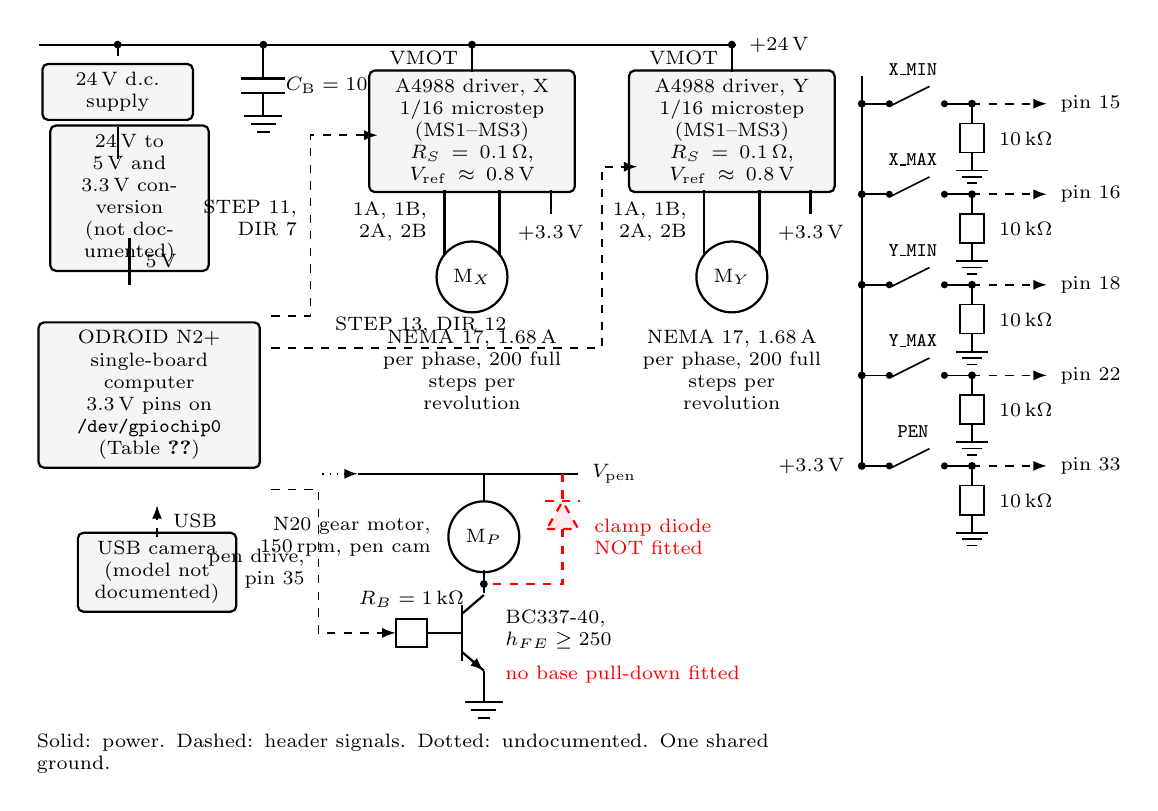
\begin{tikzpicture}[x=1cm,y=1cm,font=\scriptsize,>=latex,
  blk/.style={draw,thick,rounded corners=2pt,align=center,inner sep=3pt,fill=gray!8},
  mot/.style={draw,thick,circle,minimum size=9mm,fill=white},
  w/.style={draw,semithick},
  pw/.style={draw,thick},
  sig/.style={draw,semithick,dashed,-{Latex[length=1.7mm]}}]

%% ---------------- 24 V rail, supply, bulk capacitor ----------------
\draw[pw] (0.45,10.05) -- (9.3,10.05);
\node[anchor=west] at (9.35,10.05) {$+24$\,V};
\node[blk,text width=1.7cm] (psu) at (1.45,9.45) {24\,V d.c.\\supply};
\draw[pw] (1.45,9.9) -- (1.45,10.05);
\fill (1.45,10.05) circle (0.05);
\draw[pw] (3.3,10.05) -- (3.3,9.62);
\fill (3.3,10.05) circle (0.05);
\draw[pw] (3.02,9.62) -- (3.58,9.62);
\draw[pw] (3.02,9.44) -- (3.58,9.44);
\draw[pw] (3.3,9.44) -- (3.3,9.14);
\draw[w] (3.06,9.14) -- (3.54,9.14);
\draw[w] (3.14,9.04) -- (3.46,9.04);
\draw[w] (3.22,8.94) -- (3.38,8.94);
\node[anchor=west] at (3.46,9.53) {$C_{\mathrm B}=100$\,\textmu F};

%% ---------------- conversion, computer, camera ----------------
\node[blk,text width=1.8cm] (conv) at (1.6,8.1) {24\,V to 5\,V and\\3.3\,V conversion\\(not documented)};
\draw[pw] (1.45,9.0) -- (1.45,8.6);
\node[blk,text width=2.6cm] (sbc) at (1.85,5.6) {ODROID N2+\\single-board computer\\3.3\,V pins on\\\texttt{/dev/gpiochip0}\\(Table~\ref{tab:gan-pins})};
\draw[pw] (1.6,7.6) -- (1.6,7.0);
\node[anchor=west] at (1.68,7.3) {5\,V};
\node[blk,text width=1.8cm] (cam) at (1.95,3.35) {USB camera\\(model not\\documented)};
\draw[sig] (1.95,3.8) -- (1.95,4.2);
\node[anchor=west] at (2.03,4.0) {USB};

%% ---------------- A4988 drivers and motors ----------------
\node[blk,text width=2.4cm] (dx) at (5.95,8.95) {A4988 driver, X\\1/16 microstep\\(MS1--MS3)\\$R_S=0.1\,\Omega$,\\$V_{\mathrm{ref}}\approx0.8$\,V};
\node[blk,text width=2.4cm] (dy) at (9.25,8.95) {A4988 driver, Y\\1/16 microstep\\(MS1--MS3)\\$R_S=0.1\,\Omega$,\\$V_{\mathrm{ref}}\approx0.8$\,V};
\draw[pw] (5.95,9.7) -- (5.95,10.05);
\fill (5.95,10.05) circle (0.05);
\draw[pw] (9.25,9.7) -- (9.25,10.05);
\fill (9.25,10.05) circle (0.05);
\node[anchor=east] at (5.9,9.88) {VMOT};
\node[anchor=east] at (9.2,9.88) {VMOT};
\draw[pw] (6.95,8.2) -- (6.95,7.9);
\node[anchor=north] at (6.95,7.88) {$+3.3$\,V};
\draw[pw] (10.25,8.2) -- (10.25,7.9);
\node[anchor=north] at (10.25,7.88) {$+3.3$\,V};
\node[mot] (mx) at (5.95,7.1) {M$_X$};
\node[mot] (my) at (9.25,7.1) {M$_Y$};
\draw[pw] (5.60,8.2) -- (5.60,7.38);
\draw[pw] (6.30,8.2) -- (6.30,7.38);
\draw[pw] (8.90,8.2) -- (8.90,7.38);
\draw[pw] (9.60,8.2) -- (9.60,7.38);
\node[anchor=east,align=right] at (5.50,7.80) {1A, 1B,\\2A, 2B};
\node[anchor=east,align=right] at (8.80,7.80) {1A, 1B,\\2A, 2B};
\node[anchor=north,text width=2.4cm,align=center] at (5.95,6.55) {NEMA 17, 1.68\,A\\per phase, 200 full\\steps per revolution};
\node[anchor=north,text width=2.4cm,align=center] at (9.25,6.55) {NEMA 17, 1.68\,A\\per phase, 200 full\\steps per revolution};

%% ---------------- step and direction lines ----------------
\draw[sig] (3.4,6.6) -- (3.9,6.6) -- (3.9,8.9) -- (4.75,8.9);
\node[anchor=east,align=right] at (3.85,7.85) {STEP 11,\\DIR 7};
\draw[sig] (3.4,6.2) -- (7.6,6.2) -- (7.6,8.5) -- (8.05,8.5);
\node[anchor=south] at (5.30,6.25) {STEP 13, DIR 12};

%% ---------------- pen-lift motor and its switching stage ----------------
\draw[pw] (4.50,4.60) -- (7.30,4.60);
\draw[w,dotted,thick,-{Latex[length=1.7mm]}] (4.05,4.60) -- (4.50,4.60);
\node[anchor=west] at (7.35,4.60) {$V_{\mathrm{pen}}$};
\draw[pw] (6.10,4.60) -- (6.10,4.22);
\node[mot] (pm) at (6.10,3.80) {M$_P$};
\draw[pw] (6.10,3.38) -- (6.10,3.08);
\node[anchor=east,align=right] at (5.55,3.80) {N20 gear motor,\\150\,rpm, pen cam};
% clamp diode, drawn dashed because it is NOT fitted
\draw[red,dashed,thick] (7.10,4.60) -- (7.10,4.25);
\draw[red,dashed,thick,fill=red!8] (6.90,3.90) -- (7.30,3.90) -- (7.10,4.25) -- cycle;
\draw[red,dashed,thick] (6.88,4.25) -- (7.32,4.25);
\draw[red,dashed,thick] (7.10,3.90) -- (7.10,3.20) -- (6.10,3.20);
\fill (6.10,3.20) circle (0.05);
\node[anchor=west,align=left,red] at (7.38,3.80) {clamp diode\\NOT fitted};
% BC337-40
\draw[pw] (5.82,2.22) -- (5.82,2.94);
\draw[pw] (5.82,2.82) -- (6.10,3.06);
\draw[pw] (5.82,2.34) -- (6.10,2.10);
\draw[pw,-{Latex[length=1.7mm]}] (5.95,2.23) -- (6.10,2.10);
\draw[pw] (6.10,2.10) -- (6.10,1.70);
\draw[w] (5.86,1.70) -- (6.34,1.70);
\draw[w] (5.94,1.60) -- (6.26,1.60);
\draw[w] (6.02,1.50) -- (6.18,1.50);
\node[anchor=west,align=left] at (6.25,2.62) {BC337-40,\\$h_{FE}\ge250$};
\node[anchor=west,align=left,red] at (6.25,2.05) {no base pull-down fitted};
\draw[pw] (5.82,2.58) -- (5.38,2.58);
\draw[pw,fill=white] (4.98,2.40) rectangle (5.38,2.76);
\node[anchor=south] at (5.18,2.78) {$R_B=1\,\mathrm{k}\Omega$};
\draw[sig] (3.4,4.4) -- (4.0,4.4) -- (4.0,2.58) -- (4.98,2.58);
\node[anchor=east,align=right] at (3.95,3.40) {pen drive,\\pin 35};

%% ---------------- switch bank ----------------
\draw[pw] (10.90,4.70) -- (10.90,9.65);
\node[anchor=east] at (10.80,4.70) {$+3.3$\,V};
\foreach \h/\nm/\pn in {9.3/X\_MIN/15,8.15/X\_MAX/16,7.0/Y\_MIN/18,5.85/Y\_MAX/22,4.7/PEN/33}{
  \fill (10.90,\h) circle (0.05);
  \draw[w] (10.90,\h) -- (11.25,\h);
  \fill (11.25,\h) circle (0.045);
  \draw[w] (11.28,\h-0.02) -- (11.76,\h+0.22);
  \fill (11.95,\h) circle (0.045);
  \draw[w] (11.95,\h) -- (12.30,\h);
  \fill (12.30,\h) circle (0.05);
  \draw[w] (12.30,\h) -- (12.30,\h-0.25);
  \draw[w,fill=white] (12.15,\h-0.25) rectangle (12.45,\h-0.62);
  \draw[w] (12.30,\h-0.62) -- (12.30,\h-0.85);
  \draw[w] (12.10,\h-0.85) -- (12.50,\h-0.85);
  \draw[w] (12.17,\h-0.93) -- (12.43,\h-0.93);
  \draw[w] (12.24,\h-1.01) -- (12.36,\h-1.01);
  \node[anchor=west] at (12.52,\h-0.44) {$10\,\mathrm{k}\Omega$};
  \node[anchor=south] at (11.55,\h+0.24) {\texttt{\nm}};
  \draw[sig] (12.30,\h) -- (13.25,\h);
  \node[anchor=west] at (13.30,\h) {pin \pn};
}
\node[anchor=north west,text width=9.4cm,align=left] at (0.3,1.42) {Solid: power. Dashed: header signals. Dotted: undocumented. One shared ground.};
\end{tikzpicture}
\caption{Complete circuit with all component values. The clamp diode is dashed because it is \emph{not} fitted, and no base pull-down is fitted either; the conversion stage, the pen rail and the supply's current rating are not documented.}
\label{fig:gan-sch}
\end{figure}

Two items in the pen switching stage are design \emph{faults}, not untested ones. \emph{No clamp diode is fitted}: at turn-off the energy $\tfrac12LI^2$ stored in the motor's inductance appears as a reverse voltage that stresses the transistor and injects noise into the shared ground, a diode across the motor, cathode to supply, having simply been omitted. \emph{No base pull-down is fitted} either, so the base floats in whatever input state the pin holds at power-up. The missing diode is also the mechanism behind the end-stop behaviour of Section~\ref{sec:gan-stop}: with no clamp and a shared ground, a coil current $I$ lifts the local ground by $I\,R_{gnd}$, and the switch inputs are referred to that ground. The fix is a clamp diode across each motor and a switch return to a single ground point, not a longer debounce.

STEP, DIR and enable are driven from 3.3\,V pins with no level shifting, sound only if $3.3\,\mathrm{V}>V_{IH}$ with margin~\cite{a4988ds}. During commissioning the X axis drove to its first end-stop but the direction pin was not observed to change level on reversal, and the fault was not resolved; a level incompatibility, a wiring or configuration fault, a damaged pin and a program fault are equally consistent with it, so no cause is claimed.
\mustcomplete{Resolve the X-axis direction fault, which blocks R5 entirely. Compare $V_{IH}$ with 3.3\,V, then meter DIR at the pin and at the driver while commanding a reversal.}

\subsubsection{Step resolution, microstepping and calibration}
\label{sec:gan-res}
\label{sec:gan-timing}

Three properties of a stepper drive fix the resolution of this machine. The motors used here take 200 \emph{full steps} per revolution, so one full step is $1.8^\circ$; because position is simply the number of steps commanded, no encoder reports where the carriage actually is, which is what \emph{open-loop} control means, and the design simply trusts the step count. That trust is the assumption on which requirement R5 rests, and it fails silently if a step is ever missed. The driver subdivides each full step by \emph{microstepping}: rather than switching the two windings fully on or off, it holds them at intermediate current ratios, placing the rotor at intermediate angles. At the 1/16 setting used here, one full step becomes 16 microsteps, so a revolution is 3200 microsteps; microstepping buys resolution and smoother motion but not proportionally more accuracy, because the intermediate positions are held by the ratio of two winding currents and are therefore more sensitive to load torque than a full step is.

Equation~\ref{eq:gan-spm} gives the step resolution from 200 full steps~\cite{stepperds}, 16 microsteps~\cite{a4988ds} and $\ell_{\mathrm{rev}}=40$\,mm,
\begin{equation}
\kappa=\frac{200\cdot16}{\ell_{\mathrm{rev}}}=\frac{3200}{40}=80\ \mathrm{steps/mm},\qquad\Delta=\frac1\kappa=12.5\ \mu\mathrm{m},
\label{eq:gan-spm}
\end{equation}
which calibration replaces by each axis's measured value. Targets are \emph{absolute} step counts, $\mathrm{round}\bigl((x+5)\kappa\bigr)$ with a 5\,mm offset, differenced against the tracked position, so rounding cannot accumulate. Quantisation error is at most $\Delta/2=6.25\ \mu$m per axis, $8.8\ \mu$m combined, 57 times finer than the 0.5\,mm of R5 --- but that is the \emph{digital} resolution only, and belt stretch, backlash, missed steps, switch repeatability and pen compliance were not measured.
Equation~\ref{eq:gan-tau} gives the delay of every pulse for a move of length $d$ at feed $v_f$ over $N_{\mathrm{maj}}=\max(|n_x|,|n_y|,1)$ major-axis steps,
\begin{equation}
\tau=\max\Bigl(\frac{d/v_f}{N_{\mathrm{maj}}},\ 2\,\mu\mathrm s\Bigr),\qquad v_f=\max(F/60,\,0.1),
\label{eq:gan-tau}
\end{equation}
with $F$ in mm/min: 900 gives $\tau=833\ \mu$s (1200 steps/s), 2400 gives 312.5\,\textmu s (3200 steps/s, 60\,rpm), homing 625 steps/s or 7.8\,mm/s. Because \emph{every} pulse of both axes sleeps for $\tau$, a segment takes $(n_{\mathrm{maj}}+n_{\mathrm{min}})\tau$ and Equation~\ref{eq:gan-eff} gives the effective feed,
\begin{equation}
v_{\mathrm{eff}}=v_f\,\frac{n_{\mathrm{maj}}}{n_{\mathrm{maj}}+n_{\mathrm{min}}}\in\Bigl[\frac{v_f}{2},v_f\Bigr],
\label{eq:gan-eff}
\end{equation}
unity axis-parallel, $\tfrac12$ at $45^\circ$. There are \emph{no acceleration ramps}, so abrupt starts at 1200 to 3200 steps/s with an unknown load may lose steps~\cite{acarnley2002}. Stepping the axes independently would draw an L-shaped path, so the program interpolates with Bresenham's integer line algorithm~\cite{bresenham1965}: an error term is carried along the major axis, the major axis is pulsed every iteration and the minor axis whenever that term would go negative, and the end-stops are read before every major step. The path so produced stays within one step of the ideal straight line, about 6\,\textmu m, using integer arithmetic only.

\emph{Direction-agnostic calibration.}
\label{sec:gan-calib}
Equation~\ref{eq:gan-spm} rests on assumed transmission values and the position after power-up is unknown, so each session begins with a direction-agnostic calibration: it drives one way at 1.6\,ms per step until \emph{either} end-stop triggers, reverses, and counts the steps to the \emph{other}. That count against the hand-measured travel gives each axis its own resolution and its initial step counter by Equation~\ref{eq:gan-cal}, placing the zero 5\,mm inside the minimum switch and leaving a usable area of $194\times252$\,mm. The tightest tolerance in the hardware design falls on the hand measurement of travel: a travel error scales every commanded position in proportion, so by Equation~\ref{eq:gan-budget} the 204\,mm travel must be known to better than 0.26\,mm, or 0.13\,\%, for the scale error alone to stay inside half of R5. Appendix~\ref{sec:app-hw} derives that bound and the calibration arithmetic.

Figure~\ref{fig:gan-code} (Appendix~\ref{sec:app-hw}) gives the interpolation loop as pseudocode. The result is deliberately not stored between sessions, since a bump between sessions would silently invalidate it, and an abort refuses all jobs.

A model of the interpreter for the test word of Section~\ref{sec:gc-verify} gives 6.8\,s drawing, 10.8\,s travel and 9.1\,s dwell, 26.7\,s in all, 2.4\,s per character, being a model and not a measurement.
\mustdo{state the method and uncertainty of the $L_X$ and $L_Y$ measurement, which Equation~\ref{eq:gan-budget} requires better than 0.26\,mm; measure the positional error for R5 (the same word drawn twice and overlaid) and the return-to-zero repeatability; measure the highest feed without lost steps.}

\begin{figure}[htb]
\centering
\fbox{\parbox[c][5.5cm]{0.8\linewidth}{\centering [PLACEHOLDER --- overlay of the same word drawn twice, with the measured positional deviation annotated]}}
\captionsetup{singlelinecheck=false,justification=justified}
\caption{Placeholder: the repeatability test of requirement R5 --- the same word written twice by the gantry, scanned and overlaid, with the maximum and mean deviation between the two traces marked, to show whether the digital resolution of Equation~\ref{eq:gan-spm} is actually realised by the physical machine.}
\label{fig:gan-repeat}
\end{figure}

\subsubsection{End-stops, debounce and the pen-lift mechanism}
\label{sec:gan-stop}
\label{sec:gan-pen}

A mechanical switch does not change state cleanly: its contacts strike, separate and strike again over a few milliseconds, so a single read taken during that interval may return either level. Treating one high read as a trip would stop the machine at random, and treating the first read as final would miss a genuine trip. The standard remedy is to \emph{debounce} the input, requiring the same level on several reads spaced far enough apart to outlast the bouncing.

The pen-lift mechanism itself is a design choice justified against the alternative of a third stepper or a servo motor. A servo motor expects a continuous pulse-width-modulated position command and typically needs its own timer peripheral or a precisely timed software loop running concurrently with the gantry's own step timing, competing for the same processor cycles that generate STEP pulses. An N20 geared d.c.\ motor run in one direction only, with a cam that toggles the pen up or down every $90^\circ$ of rotation, needs only an on/off drive pulse of roughly known duration and a microswitch to confirm the result; it is cheap, widely available, has high torque at low speed through its internal gearbox for its size, and has a smaller profile than a comparable servo, at the cost of giving no absolute position, only a toggle.

All four end-stop switches and the pen switch are read before every major-axis step and every G-code line, and count as triggered only on three consecutive high reads 6\,ms apart. Three reads rather than two were needed because, with no flyback diode on a shared ground (Section~\ref{sec:gan-components}), switching noise held an input high for longer than a single re-check, so the debounce is compensating for a hardware omission as well as for contact bounce. Equation~\ref{eq:gan-latency} gives the resulting trip-to-stop latency,
\begin{equation}
t_{\mathrm{stop}}\approx\tau+(3-1)\cdot6\ \mathrm{ms}\approx13\ \mathrm{ms},
\label{eq:gan-latency}
\end{equation}
during which the carriage moves 0.2\,mm at 15\,mm/s and 0.5\,mm at 40\,mm/s, inside the 5\,mm edge tolerance. The pen-lift motor's drive pulse width was found by direct testing to be 260\,ms of rotation plus 90\,ms of settling, 350\,ms in total, rather than by calculation, since the cam geometry and the gearbox reduction were not modelled.

On a trip the program latches a stop, sets both STEP pins low, retracts off every triggered switch and aborts the job; targets are clamped to the calibrated area and the latch clears only by explicit command, refused while a switch is still triggered. Protection is \emph{software only}: no hardware stop that cuts motor power is documented, the switches are polled only during a job, no endpoint aborts a running job, and no lock prevents two simultaneous jobs. The implemented lift, planned in the proposal as a stepper, gives only pulses, so the pen state must be tracked in software, and the pen switch is feedback only (high = up); the pen-drive routine must test the switch before energising the motor, since an unnecessary pulse would toggle the pen to the wrong state rather than leave it alone.

During tuning the clicker sometimes over-rotated and the pen did not push down fully before the switch read as triggered, requiring the pulse width to be tuned empirically to the 350\,ms figure above; differing pen pressure on a book or an exam pad, rather than a flat board, also introduced inconsistent ink, so a rigid clipboard with a single page clamped flat was adopted. One pen toggle was never timed with an independent stopwatch, only inferred from the tuning above, and the generator's 0.35\,s assumption is the largest single contributor to the predicted writing time of Section~\ref{sec:gan-timing}. Neither the DIR-to-STEP timing nor the driver's minimum STEP width is modelled, and missed steps cannot be detected without feedback, so the true positional accuracy must come from the repeatability test of Figure~\ref{fig:gan-repeat}, not from Equation~\ref{eq:gan-spm} alone.
Simple-shape tests (repeating a line over itself, drawing a rectangle of known dimensions, and sending G-code produced by third-party software) were used during bring-up to verify G-code following, calibration and end-stop detection, and surfaced three problems resolved before the circuit above was finalised: end-stop priority clashing between calibration and run-time checks, generated text initially drawing backwards, and flex in the pen-lift mechanism skewing writing slightly along one axis.

\begin{figure}[htb]
\centering
\fbox{\parbox[c][4.5cm]{0.75\linewidth}{\centering [PLACEHOLDER --- scanned test rectangle with measured side lengths and diagonals annotated against the commanded dimensions]}}
\captionsetup{singlelinecheck=false,justification=justified}
\caption{Placeholder: a simple-shape test --- a rectangle of known commanded dimensions, drawn and scanned, with the measured sides and diagonals marked beside the intended values, to show the gantry's dimensional accuracy independent of handwriting.}
\label{fig:gan-rect}
\end{figure}

\subsubsection{G-code generation and the motion mapping}
\label{sec:gcode}

A pen trajectory in millimetres (Section~\ref{sec:synthesis}) has to become a machine program before the interpreter of the sections above can execute it. The format used is G-code, the command language of plotters and numerically controlled machines standardised as ISO 6983-1~\cite{iso6983}: a list of text lines, each naming a command and its arguments. Only five commands are used: \texttt{G21} and \texttt{G90} set the units to millimetres and the coordinates to absolute, \texttt{G0} is a move with the pen up and \texttt{G1} a move with the pen down, \texttt{M3} and \texttt{M5} lower and raise the pen, \texttt{G4} pauses, and \texttt{M2} ends the program. Coordinates are \emph{absolute}, so a rounding error in one move cannot accumulate into the next, and settings such as the feed rate are \emph{modal}, staying in force until another line changes them. The format splits the motion chain in two: the generator needs to know nothing about the gantry electronics, and the interpreter needs to know nothing about handwriting, with a plain-text file between them that can be inspected and replayed without the machine present.

The trajectory and the machine frame both have $X$ right and $Y$ up. For a trajectory of bounding box $(x_0,y_0,x_1,y_1)$, width $w$ and height $h$, the block is shrunk by Equation~\ref{eq:gc-map}, never enlarged, if it would leave the $200\times200$\,mm work area:
\begin{equation}
s=\min\Bigl(1,\ \frac{X_{\max}-X_{\mathrm o}}{w},\ \frac{Y_{\mathrm o}-Y_{\min}}{h}\Bigr),\qquad X=X_{\mathrm o}+(x-x_0)\,s,\quad Y=Y_{\mathrm o}-(y_1-y)\,s,
\label{eq:gc-map}
\end{equation}
with the origin $(X_{\mathrm o},Y_{\mathrm o})=(10,180)$\,mm. Each pen lift is followed by a \emph{dwell} of 350\,ms (Section~\ref{sec:gan-pen}), so a stroke costs 0.7\,s of dwell, which is why dwell dominates the predicted job time. The generator can also write a step schedule with a time estimate, assuming each move starts and ends at rest under the standard trapezoidal velocity profile used for point-to-point moves on automatic machines~\cite{biagiotti2008}, with acceleration $a=400$\,mm/s$^2$, 15\,mm/s drawing and 40\,mm/s travelling (Equation~\ref{eq:gc-trap}):
\begin{equation}
T(d)=\begin{cases}\dfrac{d}{v}+\dfrac{v}{a},&d\ge2d_a,\\[2mm]2\sqrt{\dfrac{d}{a}},&d<2d_a,\end{cases}\qquad d_a=\frac{v^2}{2a}.
\label{eq:gc-trap}
\end{equation}
For drawing $d_a=0.28$\,mm, so a typical 0.35\,mm segment is triangular and never reaches 15\,mm/s. For the test word of Figure~\ref{fig:gc-emit}, a draw path of 83.2\,mm in 239 moves and a pen-up path of 250.3\,mm in 14 moves with 26 pen pulses, the model gives 14.1\,s drawing, 7.5\,s travel and 9.1\,s dwell, 30.7\,s in all, or 2.8\,s per character for an assumed 11 characters.

The strokes are ordered by a greedy nearest-endpoint rule, grouped into text rows, so only order and direction change and the ink is identical; this is the pen-movement optimisation of R3. A program is a comment header, \texttt{G21}/\texttt{G90}, then one block per stroke at the 900\,mm/min draw feed, and finally pen up, parking and \texttt{M2}; Figure~\ref{fig:gc-emit} is the start of a generated program.

\begin{figure}[!htbp]
\centering
\fontsize{8}{9.2}\selectfont
\begin{lstlisting}[basicstyle=\ttfamily\fontsize{8}{9.2}\selectfont,frame=none]
; start of a generated program -- author yeukita
; steps/mm  X=80.000  Y=80.000 (3200 microsteps/rev)
G21   ; millimetres
G90   ; absolute
G0 F2400                     ; travel feed, emitted once
G0 X10.059 Y179.271          ; travel to the first stroke
M3   ; pen DOWN (one 90deg pulse of the one-way gear motor)
G4 P0.350   ; wait for the 90deg rotation to finish
G1 F900                      ; draw feed
G1 X10.084 Y178.920          ; one line per vertex (0.35 mm apart)
\end{lstlisting}
\caption{Start of a generated program for the test word of writer yeukita (14 strokes, 239 draw moves, vertices 0.348\,mm apart on average). The trailing comments on the motion lines are annotations added here.}
\label{fig:gc-emit}
\end{figure}

\label{sec:gc-verify}
The generator is the one stage whose output can be checked exactly, because both its input and its correct output are geometry. An independent second parser reads the finished G-code file back as though it were the machine, following $X$ and $Y$, starting a polyline at \texttt{M3} and closing it at \texttt{M5}. The trajectory that went in and the polylines that come back out are compared by Equation~\ref{eq:gc-verify}:
\begin{equation}
\mathrm{IoU}=\frac{|M_{\mathrm t}\cap M_{\mathrm g}|}{|M_{\mathrm t}\cup M_{\mathrm g}|},\qquad e_{\mathrm{mean}}=\frac{1}{J}\sum_j\min_i\lVert g_j-s_i\rVert,\qquad e_{\max}=\max_j\min_i\lVert g_j-s_i\rVert,
\label{eq:gc-verify}
\end{equation}
drawn onto a common grid of 8 pixels per millimetre for the area ratio $\mathrm{IoU}$, and sub-sampled vertex-to-vertex distances for the mean and worst case. This measures only the loss between the trajectory and the file --- rounding to three decimals, stroke reordering and work-area clamping --- and says nothing about the mechanical error of Section~\ref{sec:gan-res}, which is a separate matter. The project notes quote $\mathrm{IoU}\approx0.99$ and a text-accuracy change of at most 0.3 percentage points between direct and read-back rendering, for an earlier system state (Table~\ref{tab:syn-evid} shows later pairs); $e_{\mathrm{mean}}$ and $e_{\max}$ were never logged.
\mustdo{run the comparison for a set of generated programs and report $\mathrm{IoU}$, $e_{\mathrm{mean}}$ and $e_{\max}$; the saving produced by the stroke-ordering optimisation of R3 was not measured.}

\begin{figure}[htb]
\centering
\fbox{\parbox[c][5cm]{0.8\linewidth}{\centering [PLACEHOLDER --- the synthesised trajectory of Figure~\ref{fig:gc-emit}'s test word overlaid with the polylines re-parsed from its G-code]}}
\captionsetup{singlelinecheck=false,justification=justified}
\caption{Placeholder: the G-code verification of Equation~\ref{eq:gc-verify} --- the original trajectory and the re-parsed polylines overlaid, with the measured $\mathrm{IoU}$, $e_{\mathrm{mean}}$ and $e_{\max}$ printed beside the figure, showing the generator introduces negligible geometric loss.}
\label{fig:gc-verify-fig}
\end{figure}

\label{sec:gc-faults}
Three faults in the generator are worth stating plainly rather than left for a reader to find. The stroke rows are sorted by ascending $Y$, so a multi-line job starts with the \emph{bottom} line, not in reading order. The interpreter has one \emph{modal} feed register and no rapid mode, but the generator emits the rapid feed once at the start and the draw feed before every stroke, so pen-up travel after the first stroke runs slower than the time model assumes. Lines wrap at a width that reaches the driver's clamp boundary, which would distort the last millimetre of a full-width line.

\endgroup


\subsection{Page conditioning and line segmentation}
\label{sec:segmentation}

This subsection turns a photograph of a handwritten page into clean, deskewed, white-background line images for the text recogniser of Section~\ref{sec:textrec} and the writer classifier of Section~\ref{sec:writerid} (functional units FU~2.1 and FU~2.2; requirement R2), component by component: the array primitives the rest of the block is built from, lighting and binarisation, deskew, removal of what is not handwriting, line pitch and centres, and finally the seam cut and crop.

The deployed implementation is \texttt{SegmentLean.py}, eleven functions in about 570 lines behind a single entry point, \texttt{SegmentLines(path)}. The web server, the style-profile builder and the writer-classifier trainer all call that same entry point, so training pages are cut by exactly the code that cuts a page during normal use. Published methods are cited where they are used, and the rules around them are plain array arithmetic written for this project. No part of this block resamples through an imaging library: every operation that changes a pixel value is performed by the project's own module, implementing Equation~\ref{eq:seg-resize} directly; the library is used only to read the file from disk and to write the optional debug overlay.

\subsubsection{Design goals and the measured scale unit}

A flat-bed scan can be conditioned by grey conversion, binarisation and bounding-box line separation, which is what published pipelines do~\cite{hemanth2022,chen2023}. A photograph is harder: it adds uneven illumination, the surroundings of the sheet, skew, printed rules, edge slivers, creases, and lines that touch each other. The block therefore has three design goals: it must work at any camera resolution and any handwriting size without manual tuning, it must never delete handwriting to remove a nuisance, and it must keep as few fixed constants as possible. All three are met by letting the page set its own scale: the photograph is reduced $2{:}1$ per axis by box averaging, and the \emph{line pitch} $P$ is measured on that working image (Section~\ref{sec:seg-pitchcentres}), after which almost every threshold is a multiple of $P$ rather than an absolute pixel count. Only four constants are absolute: the blur radius, the floor of 60 ink pixels per emitted line, the $64\times640$ canvas size and the dynamic-programme weights (Table~\ref{tab:seg-const}, Appendix~\ref{sec:app-seg}).

Before any of the thresholds above can be fixed, the line itself needs a shared vocabulary. Every subsystem from here onwards measures handwriting against five quantities shown in Figure~\ref{fig:seg-geom}: the \emph{baseline}, the \emph{x-height} $x_{\mathrm h}$ (the height of a lower-case letter with no tall part and no tail), an \emph{ascender} and \emph{descender} reaching above and below that, and the \emph{line pitch} $P$, the baseline-to-baseline distance. The pitch $P$ is the unit of this block, because segmentation separates one line from the next; the x-height $x_{\mathrm h}$ is the unit of everything downstream (Sections~\ref{sec:wid-strokenorm}, \ref{sec:styleprofile}, \ref{sec:synthesis}), because measuring in x-heights removes both the camera's distance and the writer's absolute size as variables, so one stored style profile can be drawn at any pen size.

\begin{figure}[h]
\centering
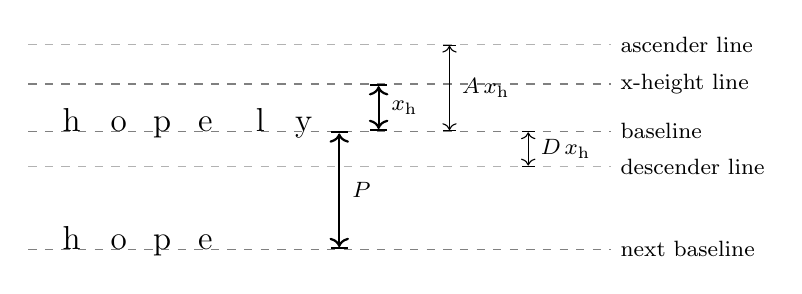
\begin{tikzpicture}[x=1cm,y=1cm,font=\footnotesize]
\draw[dashed,gray]      (0,0)    -- (7.4,0)    node[right,black]{baseline};
\draw[dashed,gray]      (0,0.6)  -- (7.4,0.6)  node[right,black]{x-height line};
\draw[dashed,gray!60]   (0,1.1)  -- (7.4,1.1)  node[right,black]{ascender line};
\draw[dashed,gray!60]   (0,-0.45)-- (7.4,-0.45)node[right,black]{descender line};
\node[anchor=base,font=\large] at (0.55,0) {h};
\node[anchor=base,font=\large] at (1.15,0) {o};
\node[anchor=base,font=\large] at (1.70,0) {p};
\node[anchor=base,font=\large] at (2.25,0) {e};
\node[anchor=base,font=\large] at (2.95,0) {l};
\node[anchor=base,font=\large] at (3.50,0) {y};
\draw[|<->|,thick] (4.45,0) -- (4.45,0.6) node[midway,right=1pt]{$x_{\mathrm{h}}$};
\draw[|<->|] (5.35,0) -- (5.35,1.1)  node[midway,right=1pt]{$A\,x_{\mathrm{h}}$};
\draw[|<->|] (6.35,0) -- (6.35,-0.45)node[midway,right=1pt]{$D\,x_{\mathrm{h}}$};
\draw[dashed,gray] (0,-1.5) -- (7.4,-1.5) node[right,black]{next baseline};
\node[anchor=base,font=\large] at (0.55,-1.5) {h};
\node[anchor=base,font=\large] at (1.15,-1.5) {o};
\node[anchor=base,font=\large] at (1.70,-1.5) {p};
\node[anchor=base,font=\large] at (2.25,-1.5) {e};
\draw[|<->|,thick] (3.95,0) -- (3.95,-1.5) node[midway,right=1pt]{$P$};
\end{tikzpicture}
\caption{The five quantities every subsystem measures handwriting against. $A>1$ because an ascender reaches above the x-height line, and $D<0$ because a descender falls below the baseline. $P$ is the unit used by this block; $x_{\mathrm h}$ is the unit used by every block after it.}
\label{fig:seg-geom}
\end{figure}

\subsubsection{Array primitives: summed-area tables and run tests}

Almost every operation in this block is a sum, a maximum, or a test of whether anything is set, taken over a rectangular window. Computed directly, a window of radius $r$ costs $O(r)$ per pixel per axis, too slow here because the illumination blur below uses a radius of up to 40 pixels. The module therefore builds a summed-area table~\cite{crow1984}, also called an integral image, in one $O(HW)$ pass of two cumulative sums, after which the sum over a window of \emph{any} size costs four look-ups instead of $(2r+1)^2$ additions. Three stages of this block resample an image, and each does so by bilinear interpolation at the source position given by Equation~\ref{eq:seg-resize}, the one exception being an ownership map resampled by nearest neighbour, because its values are integer line indices that interpolation would invent new values for:
\begin{equation}
y_s=\frac{(i+0.5)\,h}{h'}-0.5,\quad x_s=\frac{(j+0.5)\,w}{w'}-0.5,\quad I'(i,j)=\sum_{a,b\in\{0,1\}}\omega_{ab}\,I(\lfloor y_s\rfloor+a,\lfloor x_s\rfloor+b).
\label{eq:seg-resize}
\end{equation}

The table itself is the running two-dimensional sum of the image,
\begin{equation}
S(y,x)=\sum_{i<y}\sum_{j<x} I(i,j),
\label{eq:seg-sat}
\end{equation}
where $S$ is the summed-area table and $I$ the image being summed. Equation~\ref{eq:seg-sat} is built once per image. Any window sum is then read from four of its entries,
\begin{equation}
\mathrm{BoxSum}=S(y_2,x_2)-S(y_1,x_2)-S(y_2,x_1)+S(y_1,x_1),
\label{eq:seg-boxsum}
\end{equation}
where $y_2=y_1+2r+1$ and $x_2=x_1+2r+1$ are the far corners of a window of radius $r$, the array having been padded by $r$ with edge replication beforehand. The cost of Equation~\ref{eq:seg-boxsum} does not depend on $r$, which is what makes the radius-40 illumination blur of Section~3.4.3 affordable.

The same cumulative trick gives the two binary operations the block needs. A dilation along one axis is
\begin{equation}
\mathrm{AnyWithinRadius}(m,r)[i]=\bigl[\,c[i+2r+1]-c[i]>0\,\bigr]=\Bigl[\textstyle\bigvee_{k=-r}^{r} m[i+k]\Bigr],
\label{eq:seg-dilate}
\end{equation}
where $m$ is the binary mask, $c$ its cumulative sum and $r$ the radius. Equation~\ref{eq:seg-dilate} is a dilation because the bracket is true exactly when at least one pixel within $r$ is set. A square dilation separates into two applications of it, one per axis, so it costs the same at any radius. An erosion is the complemented dilation of the complement, and a closing is a dilation followed by an erosion, so no other structuring element has to be implemented. The second operation marks long runs,
\begin{equation}
\mathrm{LongRun}(m,n)[j]=\bigl[\,\mathrm{ch}[h_j+1]-\mathrm{ch}[l_j]>0\,\bigr],\qquad l_j=\max(0,j-n+1),\quad h_j=\min(j,L-n),
\label{eq:seg-runmask}
\end{equation}
where $n$ is the minimum run length, $\mathrm{ch}$ the cumulative count of positions at which a run of $n$ consecutive set pixels begins, $L$ the length of the axis, and $l_j,h_j$ the first and last such start positions that could cover index $j$. Equation~\ref{eq:seg-runmask} is true at every pixel lying on a run of at least $n$ set pixels, and is used by Section~\ref{sec:seg-cleanup} to find printed rules. Figure~\ref{fig:seg-primspseudo} (Appendix~\ref{sec:app-seg}) gives all three as pseudocode. Only one true Gaussian filter is used, a 25-tap kernel smoothing the row profile of Section~\ref{sec:seg-pitchcentres} with $\sigma=4$ rows, about a tenth of a typical pitch.

\subsubsection{Lighting normalisation and binarisation}

The intensity measured by a camera is approximately the reflectance of the paper multiplied by the illumination falling on it. Because the nuisance term is a multiplication and not an addition, it is divided out rather than subtracted: the working grey image $G$ is divided by a single box mean of itself, giving a ratio image $\rho$ close to 1 on paper whatever the lighting, and on ink the ink-to-paper reflectance ratio of the pen itself. Once the shading is divided out, the ink decision is a single global threshold, chosen by Otsu's method~\cite{otsu1979}, which is possible only because of the division --- this is the step that removed the long chain of clean-up filters the project's first segmenter needed.

The ratio image is formed by dividing the grey image by a box mean of itself,
\begin{equation}
\rho(p)=\frac{G(p)}{\max\bigl(\mathrm{BoxMean}_r(G)(p),\,1\bigr)},
\label{eq:seg-flat}
\end{equation}
where $\rho(p)$ is the ratio at pixel $p$, $G$ the working grey image and $\mathrm{BoxMean}_r$ the mean over a window of radius $r$, evaluated through Equation~\ref{eq:seg-boxsum}. The denominator is floored at 1 so a black border cannot divide by zero. The radius is tied to the image height,
\begin{equation}
r=\max\bigl(8,\;\min(40,\;\mathrm{round}(H/41))\bigr),
\label{eq:seg-flatradius}
\end{equation}
where $H$ is the height of the working image in rows. Equation~\ref{eq:seg-flatradius} makes the background estimate cover the same fraction of the page at any camera resolution. The radius must be much larger than a letter, or letters would darken their own background estimate and be divided away; the bounds of 8 and 40 rows keep it so at the resolutions used here.

The threshold separating ink from paper is then the one that best splits the histogram of $\rho$ into two groups, by Otsu's criterion~\cite{otsu1979},
\begin{equation}
t^*=\arg\max_t\;\omega_B(t)\,\omega_F(t)\,\bigl[\mu_B(t)-\mu_F(t)\bigr]^2 ,
\label{eq:seg-otsu}
\end{equation}
where $t^*$ is the chosen threshold, $\omega_B(t)$ and $\omega_F(t)$ are the fractions of pixels below and above a candidate $t$, and $\mu_B(t)$ and $\mu_F(t)$ are their means. The quantity maximised in Equation~\ref{eq:seg-otsu} is the between-class variance, and it is evaluated for all 256 histogram bins at once. A pixel is marked as ink when $\rho<t^*$. Applying Equation~\ref{eq:seg-otsu} globally is defensible only because Equation~\ref{eq:seg-flat} has already removed the shading that would otherwise force a local threshold.

One extra test is needed beyond the threshold: a solid-area veto removes any window entirely ink, since no pen stroke fills a $9\times9$ window, which catches a binder shadow or the dark gutter of a bound book. The whole stage is four array statements (Figure~\ref{fig:seg-inkpseudo}, Appendix~\ref{sec:app-seg}).

\begin{figure}[htb]
\centering
\fbox{\parbox[c][4.5cm]{0.8\linewidth}{\centering [PLACEHOLDER --- four-panel figure: photograph, grey image, blurred background estimate, ratio image $\rho$]}}
\captionsetup{singlelinecheck=false,justification=justified}
\caption{Placeholder: the four stages of Equation~\ref{eq:seg-flat} on one real page --- the photograph, its grey conversion, the box-mean background estimate, and the resulting ratio image $\rho$, showing the shading removed before Otsu's threshold is applied, from \texttt{InkMask}.}
\label{fig:seg-flat-fig}
\end{figure}

\subsubsection{Deskew by searching rotations}

When text lines are horizontal, the row-sum profile of the ink has sharp peaks at the line bodies and deep troughs between them; any tilt smears those peaks, since a single row then cuts across several lines. This projection-profile approach to skew detection~\cite{postl1986} is a standard alternative to a Hough transform over ink edges~\cite{duda1972}, chosen here because a page of handwriting and printed rules gives the Hough transform many competing line candidates, whereas the row profile already favours the direction most of the ink actually runs in. The sharpness of the profile is therefore a measure of how level the page is, and can be maximised directly.

The row profile at a trial angle is the ink count per row,
\begin{equation}
P_\theta(y)=\sum_x R_\theta(y,x),
\label{eq:seg-profile}
\end{equation}
where $P_\theta(y)$ is the number of ink pixels in row $y$ and $R_\theta$ is the ink mask notionally rotated by $\theta$. The sharpness of Equation~\ref{eq:seg-profile} is scored by its sum of squares, and the angle maximising that score is taken,
\begin{equation}
J(\theta)=\sum_y P_\theta(y)^2,\qquad \theta^*=\arg\max_\theta J(\theta),
\label{eq:seg-skew}
\end{equation}
where $J(\theta)$ is the objective and $\theta^*$ the chosen skew angle. Squaring before summing is what makes Equation~\ref{eq:seg-skew} work: the total amount of ink does not change under rotation, so $\sum_yP_\theta(y)$ is fixed, whereas the sum of squares is largest when the same ink is concentrated into the fewest rows, which happens when the lines are level.

The rotation is never performed to score a candidate. Each ink pixel is mapped straight to the row it would land in,
\begin{equation}
k=(y-c_y)\cos\theta-(x-c_x)\sin\theta+c_y,
\label{eq:seg-skewrow}
\end{equation}
where $k$ is that row index, $(y,x)$ the pixel's coordinates and $(c_y,c_x)$ the image centre. Counting rows through Equation~\ref{eq:seg-skewrow} was measured 31 times faster than rotating the mask seventeen times.

The search sweeps 17 candidate angles from $-4^\circ$ to $+4^\circ$ in steps of $0.5^\circ$ on the stage-2 mask reduced by a further factor of two, with no refinement pass, so the best accuracy reachable is half a step, $0.25^\circ$. Ink that would fall outside the row range at a trial angle is allowed to extend the profile rather than being clipped, since clipping piles out-of-range pixels into one row whose artificial spike scores higher than any real text line; an earlier version with this clipping fault chose an angle four degrees wrong on a tilted page. Only once an angle is chosen is the page itself rotated, bilinearly, and the ink mask and ratio image recomputed, because Equation~\ref{eq:seg-flat} is not rotation-equivariant.

Table~\ref{tab:seg-test} (Section~\ref{sec:seg-test}) reports the deskew measurement: seven angles on the search grid recovered exactly in 35 of 35 trials, and four angles between grid points recovered to $0.25^\circ$, exactly half the search step, in 20 of 20 trials, showing the stage is limited by the coarseness of its own search grid and not by the objective.

\subsubsection{Removing what is not handwriting}
\label{sec:seg-cleanup}

Three kinds of nuisance are removed in turn, each identified by a property that handwriting does not share. The area outside the sheet is removed because handwriting disappears under a coarse enough average while the sheet itself does not. Printed structure --- ruled paper, underlines, a bound book's spine shadow --- is removed because it runs straight for longer than a line spacing, which handwriting does not, a long directional opening rather than a fixed-size filter. Edge slivers, corner shadows and creases are removed because, although not straight, they are judged as whole connected pieces rather than pixel by pixel: each fragment is labelled by the same connected-component logic used throughout this block, and the whole piece is then scored on being long and thin or sparse inside its own bounding box.

The long-run primitive of Equation~\ref{eq:seg-runmask}, bracketed by a dilation and a re-intersection with the real ink, gives Equation~\ref{eq:seg-cand} for flat (horizontal) and upright (vertical) printed structure, where $\mathcal D_r^{y}$ and $\mathcal D_r^{x}$ are one-axis dilations:
\begin{equation}
\begin{aligned}
\mathrm{flat}&=\mathcal D_{1}^{y}\Bigl(\mathrm{LongRun}^{x}\bigl(\mathcal D_{1}^{y}(\mathrm{ink}),\;\lfloor1.25P\rfloor\bigr)\Bigr)\wedge\mathrm{ink},\\
\mathrm{upright}&=\mathcal D_{3}^{x}\Bigl(\mathrm{LongRun}^{y}\bigl(\mathcal D_{3}^{x}(\mathrm{ink}),\;\lfloor1.4P\rfloor\bigr)\Bigr)\wedge\mathrm{ink}.
\end{aligned}
\label{eq:seg-cand}
\end{equation}
The two run lengths, $1.25P$ horizontally and $1.4P$ vertically, are longer than any single letter can be, so no letter is mistaken for a rule; the dilation before the run test tolerates a slight tilt, and the re-intersection means only real ink is ever removed.

Separating ink into pieces for the third kind of nuisance needs connected-component labelling: every set pixel is given an integer label, two pixels sharing a label when a path of set pixels joins them. The mask is closed first so pen lifts inside a word are bridged, and the labelling is a run-length union-find pass, each row reduced to its horizontal runs before a union-find structure records which runs belong together, so the whole page is labelled in one pass over the rows. Every discard statistic is accumulated over the \emph{original} ink pixels, not the closed mask, so closing can join pieces but never add area to a decision; eight discard predicates combine size, aspect ratio, faintness and distance from the frame (Table~\ref{tab:seg-artifact}, Appendix~\ref{sec:app-seg}). The most aggressive discards any piece within $\max(3,\lfloor0.5P\rfloor)$ of the left frame edge, which removes the facing page of an open book but costs the first letters of a page with no left margin.

\begin{figure}[htb]
\centering
\fbox{\parbox[c][4cm]{0.75\linewidth}{\centering [PLACEHOLDER --- ruled page before and after rule removal]}}
\captionsetup{singlelinecheck=false,justification=justified}
\caption{Placeholder: a page of ruled paper before and after Equation~\ref{eq:seg-cand} removes the printed rules, confirming that handwriting crossing a rule survives while the rule itself is removed.}
\label{fig:seg-rules}
\end{figure}

\subsubsection{Line pitch and line centres}
\label{sec:seg-pitchcentres}

The row-ink profile is the mask pixel count per row over a central window, smoothed by the Gaussian kernel of Section 3.4.2:
\begin{equation}
\mathrm{prof}(y)=\sum_{x=\lfloor0.05W\rfloor}^{\lfloor0.97W\rfloor-1}\mathrm{ink}(y,x),\qquad \mathrm{sm}=\mathrm{prof}*k,
\label{eq:seg-pitch}
\end{equation}
where $\mathrm{prof}(y)$ is the ink count in row $y$, $W$ is the image width, $k$ is the 25-tap Gaussian kernel of Section~3.4.2 and $\mathrm{sm}$ the smoothed profile. The window in Equation~\ref{eq:seg-pitch} excludes the outer five per cent on the left and three per cent on the right, where a binding shadow or a torn edge would otherwise contribute a constant to every row.

A line centre is a peak of $\mathrm{sm}$ satisfying three conditions together,
\begin{equation}
\mathrm{sm}(y)\ge\mathrm{sm}(y-1),\qquad \mathrm{sm}(y)>\mathrm{sm}(y+1),\qquad \mathrm{sm}(y)>0.06\max_u\mathrm{sm}(u),
\label{eq:seg-centres}
\end{equation}
where $y$ is a candidate row. The comparisons in Equation~\ref{eq:seg-centres} are deliberately asymmetric, one non-strict and one strict, so the last row of a flat-topped peak is taken exactly once. The relative floor of $0.06$ scales with the amount of ink on the page rather than being an absolute count, so a faint page is not rejected wholesale.

The pitch is the median of the gaps between consecutive peaks, used whenever at least two peaks exist; a median rather than a mean so one unusually large gap, such as a paragraph break, cannot shift it. Three fallbacks follow in order when fewer than two peaks are found: the \emph{autocorrelation} of the profile, whose first strong lag in a stated range is taken as the pitch; failing that, an estimate from the median connected-component height, $P=\max(15,\mathrm{round}(2.2\,\mathrm{median}\{h_c\}))$; and, with no usable components either, a fixed 48 rows (Figure~\ref{fig:seg-pitchpseudo}, Appendix~\ref{sec:app-seg}). The pitch and profile are recomputed on the cleaned mask after Section~\ref{sec:seg-cleanup}, and the peaks become line centres through greedy non-maximum suppression, a peak accepted only if it lies at least $0.6P$ from every centre already accepted.

Table~\ref{tab:seg-test} reports the line-count test below.

\subsubsection{Seam cut, pixel ownership and the final crop}

A straight cut halfway between two line centres would sever every descender and ascender that crosses it, so the boundary between two lines must bend around the ink. The two layers of ink recovery --- a strict page-wide mask and a looser threshold trusted only next to ink a line already owns --- exist because a threshold loose enough to catch a faint stroke is also loose enough to catch a shadow, and \emph{hysteresis}, using two thresholds instead of one, is the standard remedy, the same principle used to link edges in edge detection applied here to ink.

The boundary itself is found the way a seam is found in content-aware image resizing: the cheapest vertical path across a cost image, found column by column with dynamic programming rather than guessed as a straight line~\cite{avidan2007}. Between consecutive centres $c_0<c_1$ the cost field of Equation~\ref{eq:seg-cost2} and the dynamic-programme recursion of Equation~\ref{eq:seg-seam} give the cheapest path across it:
\begin{equation}
C(y,x)=4.0\,\tilde m(y,x)+0.012\left(\frac{y-\mu}{\max(1,(c_1-c_0)/2)}\right)^{\!2},\qquad \mu=c_0+\tfrac12(c_1-c_0),
\label{eq:seg-cost2}
\end{equation}
where $C(y,x)$ is the cost of placing the boundary at row $y$ of column $x$, $\tilde m$ is the dilated ink mask, and $\mu$ is the midline between the two centres $c_0$ and $c_1$. The two weights in Equation~\ref{eq:seg-cost2} are three hundred to one: crossing a single ink pixel costs 4.0 against a maximum of 0.012 for sitting a half-gap away from the midline, so the midline term only breaks ties across blank gaps between words and never persuades the seam to cut a letter.

The cheapest path is accumulated column by column,
\begin{equation}
A(y,x)=C(y,x)+\min_{|d|\le s}\bigl[\,A(y+d,\,x-1)+0.02\,|d|\,\bigr],\qquad A(y,0)=C(y,0),
\label{eq:seg-seam}
\end{equation}
where $A(y,x)$ is the cost of the cheapest path reaching $(y,x)$, $d$ is the row step taken between adjacent columns and $s=7$ bounds it. The penalty $0.02\,|d|$ in Equation~\ref{eq:seg-seam} prices vertical movement, so the seam prefers to stay level unless ink gives it a reason to climb.

The crop is then composited from its layers by a hysteresis rule,
\begin{equation}
\alpha=\max\Bigl(\alpha_{\mathrm{strong}},\ \ \mathbb 1[\rho_{\mathrm{local}}<t^*_{\mathrm{local}}]\cdot\alpha_{\mathrm{halo}}\cdot\mathbb 1[\text{not owned by another band}]\Bigr),
\label{eq:seg-hyst}
\end{equation}
where $\alpha$ is the opacity written into the crop, $\alpha_{\mathrm{strong}}$ comes from the page-wide mask, $\alpha_{\mathrm{halo}}$ from the looser local threshold $t^*_{\mathrm{local}}$, and $\mathbb 1[\cdot]$ is 1 when its condition holds and 0 otherwise. The second term of Equation~\ref{eq:seg-hyst} is the loose layer, admitted only next to ink the band already owns, which is the hysteresis: a faint stroke touching known ink is kept, while an equally faint shadow elsewhere is not.

Finally the crop's contrast is stretched,
\begin{equation}
\ell=\mathrm{clip}\!\left(\frac{255\,(v-b)}{\max(w-b,1)},0,255\right),\qquad
\mathrm{out}=255\Bigl(1-\bigl(\tfrac{255-\ell}{255}\bigr)^{0.55}\Bigr),
\label{eq:seg-stretch}
\end{equation}
where $v$ is the input grey value, $b$ and $w$ are the black and white points taken from the crop's own histogram, $\ell$ is the linearly stretched value and $\mathrm{out}$ the value written. The exponent $0.55$ in Equation~\ref{eq:seg-stretch} thickens thin strokes slightly, which matters because the recogniser was trained on ink of a similar weight.

The two outermost boundaries are fixed at $\lfloor0.75P\rfloor$ beyond the first and last centre, so $L$ centres give exactly $L$ bands; the whole computation is $O(15HW)$ at worst, the most expensive single step in the block. A pixel belongs by default to the band it lies in; six correction rules on top return a cut-off tail to the band holding most of its piece, place a small fragment by proximity, and follow a dot or accent down to its stem (Table~\ref{tab:seg-own}, Appendix~\ref{sec:app-seg}). Each crop is rendered from the full-resolution page and composited from three layers: the band's own ink mask, a recovery mask from re-applying Equations~\ref{eq:seg-flat} and~\ref{eq:seg-otsu} inside the crop alone, and the halo of the band's own strong ink. Outside the mask the crop is pure white, and it is shifted so the first inked column sits at a fixed offset, since the recogniser's input is left-flush (Equation~\ref{eq:seg-clf}):
\begin{equation}
s=\min\!\Bigl(\frac{64}{h},\frac{640}{w}\Bigr),\qquad h'=\max(1,\mathrm{round}(hs)),\qquad w'=\max(1,\mathrm{round}(ws)).\label{eq:seg-clf}
\end{equation}

\subsubsection{Testing the segmentation block}
\label{sec:seg-test}

Two properties of this block were tested against a known answer on the 30 photographed pages of the five personal writers, $2448\times3264$ pixels each. Table~\ref{tab:seg-test} gives the results: the block found the correct number of lines on all 30 pages, 669 of 669 lines, with no page over- or under-segmented, against the hand-typed transcription; and the deskew of Equation~\ref{eq:seg-skew} recovered seven grid-aligned injected angles exactly in 35 of 35 trials and four off-grid angles to $0.25^\circ$ in 20 of 20 trials.

\begin{table}[h]
\centering
\fontsize{9}{11}\selectfont
\setlength{\tabcolsep}{4pt}
\begin{tabularx}{\linewidth}{|p{4.3cm}|p{3.3cm}|X|}
\hline
\textbf{Measurement} & \textbf{Result} & \textbf{What it shows} \\
\hline
Line count against the hand-typed transcription, 30 pages & \textbf{30 of 30} pages exact; 669 of 669 lines & The line separation is correct on every page tested, and the relative floor of Equation~\ref{eq:seg-centres} lost no line. \\
\hline
Deskew, 7 angles on the search grid, 5 pages & \textbf{35 of 35} exact & The objective of Equation~\ref{eq:seg-skew} picks the correct grid point every time. \\
\hline
Deskew, 4 angles between grid points, 5 pages & \textbf{20 of 20} at $0.25^\circ$ & The residual error is exactly half the search step, so the stage is quantisation-limited, not objective-limited. \\
\hline
Time per page, $2448\times3264$ & \textbf{4.9 to 9.7\,s}, mean 7.9\,s & The cost of the deployed module. Measured with the project's own resampling throughout. \\
\hline
Measured line pitch $P$ & 47 to 58 pixels & The scale unit varies by 23\,\% across these writers, which is what the block is designed to absorb. \\
\hline
Chosen skew angle on the unrotated pages & $-1.5^\circ$ to $+3.0^\circ$ & Real photographs are tilted by more than a degree, so the stage is doing necessary work. \\
\hline
\end{tabularx}
\caption{Measured performance of the deployed segmentation block over the 30 photographed pages of the five personal writers. These are the pages the system was built on, not an unseen test set, so the line-count result shows that the block handles the material it was designed for and not that it generalises to new conditions.}
\label{tab:seg-test}
\end{table}

The 30 pages are the pages the system was built on, so the line-count result is not an unseen test; the deskew result is stronger, since the injected angle is ground truth no part of the design could have been fitted to. The timing figure also corrects an attribution: the 24.8 to 69.1\,s per page reported in Section~\ref{sec:results} is the retired segmenter, \texttt{SegmentPage.ProcessPage}; the deployed module is roughly five times faster at 4.9 to 9.7\,s, because it makes one pass over a half-resolution image where the retired module made four passes over a larger one. The mean of 7.9\,s is still about four times the two seconds requirement R4 allows for capture and conditioning. Using the project's own resampling rather than the imaging library's compiled resampling costs about 40\,\% of the block's run time, the measured price of the library-free claim.
\mustdo{update the segmentation figures of Section~\ref{sec:results} and the R4 budget to 4.9--9.7\,s; time \texttt{SegmentLean.SegmentLines} on the ODROID N2+; produce the four figures placeholdered above, plus the paper-region mask and the \texttt{\_cuts\_overlay.jpg} that \texttt{SegmentLean.py} already writes.}

\begin{figure}[htb]
\centering
\fbox{\parbox[c][5cm]{0.85\linewidth}{\centering [PLACEHOLDER --- one full page with the final seam cuts overlaid in colour, from \texttt{SegmentLean.py}'s own debug output]}}
\captionsetup{singlelinecheck=false,justification=justified}
\caption{Placeholder: the seam-cut overlay (\texttt{\_cuts\_overlay.jpg}) on one real, photographed page, showing each line's final boundary bending around ascenders and descenders rather than cutting straight through them.}
\label{fig:seg-cuts}
\end{figure}

\subsubsection{Design alternatives and limitations}

Table~\ref{tab:seg-alt} sets the main design choices against the alternatives considered. The project's first segmenter, \texttt{SegmentPage.py}, was about 2200 lines and sixty functions against the eleven here; it resized every photograph to a fixed long side, thresholded locally, removed printed structure in four passes, took a median glyph height as its scale unit, scored components for being diagrams, chained them into lines and deskewed each line separately. No part of the deployed pipeline calls it any more, and three of its capabilities were given up with it: diagram tagging, per-line deskew, and a wider $\pm8^\circ$ search at $0.1^\circ$.

\begin{table}[h]
\centering
\fontsize{8.5}{10.2}\selectfont
\setlength{\tabcolsep}{4pt}
\begin{tabularx}{\linewidth}{|p{2.4cm}|X|}
\hline
\textbf{Decision} & \textbf{Alternatives, and why the deployed choice was made} \\
\hline
Lighting & Subtracting a blurred background leaves contrast dependent on brightness. The nuisance is multiplicative, so dividing gives an ink-to-paper ratio independent of the lamp. \\
\hline
Ink threshold & A local mean less an offset marks something even in an empty region and needs a tuned offset. After the division, one global Otsu threshold is enough. \\
\hline
Scale unit & A median glyph height is upset by a heading in another size; a fixed-size page throws away resolution. The pitch $P$ is measured on the page itself. \\
\hline
Lines & Chaining components along a baseline curve needs a correct set of components first, propagating every clean-up error. The row profile yields the pitch and centres together in one $O(N_p)$ pass. \\
\hline
Line boundaries & A straight cut at the midline severs descenders and ascenders. The least-ink seam bends around them. \\
\hline
Skew & A Hough transform of ink edges~\cite{duda1972} is dominated by ruled lines and diagram strokes. The projection objective is also the quantity the pitch stage goes on to use, so it costs nothing extra. \\
\hline
Rule removal & A long morphological opening erases underlines and cannot follow a slope. The dilated long-run test needs two constants where chaining fragments across gaps needs five. \\
\hline
Not implemented & Text-versus-diagram tagging, per-line deskew and a four-point perspective warp are all absent; the first is accepted for plain prose pages, the residual drift is tolerated downstream, and the camera looks straight down. \\
\hline
\end{tabularx}
\caption{Design alternatives of the deployed segmentation block. The last row records capabilities of the first segmenter that were deliberately given up.}
\label{tab:seg-alt}
\end{table}

The block assumes left-to-right writing in a single column of roughly horizontal lines, and the following limitations follow from that design. Skew beyond $\pm4^\circ$ is not corrected at all, and up to $0.25^\circ$ always remains. Two columns of text, or a diagram beside the text, produce profile peaks that belong to no single line, and an untagged diagram is cut into line-shaped crops and read as nonsense. A line peaking below six per cent of the strongest is lost silently, although no such line occurred in the 30 pages tested. A blank page raises an exception rather than returning no lines. Illumination varying faster than the radius of Equation~\ref{eq:seg-flat} leaves one side of a hard shadow edge mis-thresholded, page curl and perspective are untreated, and colour is treated like black ink because the module is monochrome throughout.


\subsection{Text recognition and writer identification}
\label{sec:textrec}
\label{sec:writerid}

This subsection describes the two neural networks that read a handwritten line into text and decide which of the thirteen stored writers wrote it (functional unit FU~2.3; requirements R1, R2), component by component: the convolutional backbone the two share, the sequence model and alignment-free loss that make text recognition possible at all, the writer-identification head and the stroke normalisation it depends on, and the from-scratch training and verification of every layer. No machine-learning library is used anywhere in this subsection: the forward passes, the backward passes and the optimiser updates are all evaluated by one module written for this project, \texttt{NumpyNN.py} (Section~\ref{sec:textrec-numpynn}).

Both networks follow the layer pattern of Kizilirmak and Yanikoglu~\cite{kizilirmak2023}, chosen because it was evaluated on the public handwriting database used here~\cite{marti2002} and reports accuracies in the range R2 needs. That paper describes an approach and a layer pattern rather than publishing code, so the network was built from its description: the layer pattern, filter counts and recurrent width are taken from it, while the input geometry, data pipeline, label cleaning, augmentation and staged training recipe were decided for this project. That hybrid of convolution and recurrence is the combination reported to improve feature extraction and contextual understanding together~\cite{kumar2024,ma2023}.

\subsubsection{The shared convolutional backbone}
\label{sec:rec-backbone}

A convolutional neural network (CNN) is a stack of layers each of which applies the same small learned filter at every position of its input~\cite{lecun1998,yahya2021}. Applying one filter everywhere, rather than learning a separate weight for every pixel, is what makes the layer useful for handwriting: a stroke junction means the same thing wherever on the line it appears, so the filter that detects it should not have to be learned again for each position. A single convolutional layer only sees a small local neighbourhood, but stacking several lets later layers combine the simple strokes earlier layers detect into the more complex shapes of whole letters, which is why depth rather than one wide layer is used. Three further layer types complete the pattern used here, each solving a specific problem of training a deep stack: \emph{batch normalisation}, the \emph{rectifier} nonlinearity, and \emph{pooling}.

A convolution with kernel size $k$, stride $s$ and $p$ rows and columns of zero padding on each side of input $X_{\mathrm{pad}}$ is
\begin{align}
Y[o,i,j]&=b_o+\sum_{c=1}^{C_{\mathrm{in}}}\sum_{u=0}^{k-1}\sum_{v=0}^{k-1}W[o,c,u,v]\;X_{\mathrm{pad}}[c,\,s\,i+u,\,s\,j+v],\label{eq:rec-conv}\\
Y&=\tilde W\,\mathrm{cols}+b\,\mathbf 1^{\top}.\label{eq:rec-im2col}
\end{align}
Equation~\ref{eq:rec-conv} is six nested summations, too slow in array arithmetic, so the implementation uses the \emph{im2col} rearrangement of Equation~\ref{eq:rec-im2col}: every $k\times k$ patch the filter would see is copied out as one column, the filter weights reshaped into rows, and the whole convolution becomes a single matrix product, agreeing with the direct form to about $10^{-13}$ and about ten times faster. With $k=3$, $p=1$, $s=1$ the output keeps the input's height and width, so only pooling layers change the tensor size. Batch normalisation~\cite{ioffe2015} (Equation~\ref{eq:rec-bn}) rescales each channel to zero mean and unit variance over the current training batch and then applies a learned scale $\gamma$ and shift $\beta$; at inference, with no batch to average over, running statistics collected during training replace $\mu_B,\sigma_B^2$ and the whole operation folds into the single affine map of Equation~\ref{eq:rec-bnfold}:
\begin{align}
\hat x&=\frac{x-\mu_B}{\sqrt{\sigma_B^2+\varepsilon}},\qquad y=\gamma\hat x+\beta,\qquad\varepsilon=10^{-5},\label{eq:rec-bn}\\
a&=\frac{\gamma}{\sqrt{\sigma^2_{\mathrm{run}}+\varepsilon}},\qquad b=\beta-a\,\mu_{\mathrm{run}},\qquad y=a\,x+b.\label{eq:rec-bnfold}
\end{align}
The rectifier is $\max(0,x)$~\cite{nair2010}: some nonlinearity is essential, because a stack of purely linear layers collapses into one linear layer however deep it is, and the rectifier's derivative of 0 or 1 neither saturates nor shrinks the gradient across twelve layers. Max-pooling takes the largest value in each $2\times2$ window, stride 2, halving both axes with no learned parameters~\cite{ji2021}; it discards three quarters of the positions, keeping the network small enough for the target hardware, and tolerates a one-pixel shift, since moving a stroke slightly usually does not change which value in its window is largest.

Figure~\ref{fig:rec-arch} gives the three convolutional stages (32, 64 and 128 channels, 2, 4 and 6 layers respectively) with two intervening max-pools, each verified for this project against the published pattern; what follows the backbone differs between the two networks and is given in Sections~\ref{sec:rec-ctc} and~\ref{sec:wid-head}. The full recogniser holds 3\,358\,763 trainable parameters, of which the recurrent layers hold 70.5\,\% and the third convolutional stage 24.2\,\% (Table~\ref{tab:rec-layers}, Appendix~\ref{sec:app-rec}); these shapes cost $4.17\times10^9$ multiply--accumulates per line, $3.79\times10^9$ of them convolutional, so the convolutions dominate the arithmetic even though the recurrent layers hold most of the parameters.

\begin{figure}[h]
\centering
\begin{tikzpicture}[x=1cm,y=1cm,scale=0.86,transform shape]
\tikzset{nb/.style={w2box,text width=2.55cm,minimum height=1.5cm}}
\node[nb] (in) at (-6.2,0) {\textbf{Input}\\ $1\times64\times640$};
\node[nb] (s1) at (-3.1,0) {\textbf{Stage 1}\\ 2$\times$[conv 3$\times$3, BN, ReLU], 32 ch.\\ $32\times64\times640$};
\node[nb] (p1) at (0,0) {\textbf{Max-pool 2$\times$2}\\ $32\times32\times320$};
\node[nb] (s2) at (3.1,0) {\textbf{Stage 2}\\ 4$\times$[conv, BN, ReLU], 64 ch.\\ $64\times32\times320$};
\node[nb] (p2) at (6.2,0) {\textbf{Max-pool 2$\times$2}\\ $64\times16\times160$};
\node[nb] (s3) at (6.2,-2.3) {\textbf{Stage 3}\\ 6$\times$[conv, BN, ReLU], 128 ch.\\ $128\times16\times160$};
\node[nb] (hm) at (3.1,-2.3) {\textbf{Height max-pool}\\ $128\times1\times160$\\ $\rightarrow$ 160 vectors};
\node[nb] (ls) at (0,-2.3) {\textbf{text: BiLSTM $\times2$}\\ \textbf{writer: pool + head}\\ (Sections~\ref{sec:rec-ctc}, \ref{sec:wid-head})};
\foreach \a/\b in {in/s1,s1/p1,p1/s2,s2/p2,p2/s3,s3/hm,hm/ls} \draw[w2arr] (\a)--(\b);
\end{tikzpicture}
\caption{The shared convolutional backbone, the layer pattern being that of Kizilirmak and Yanikoglu~\cite{kizilirmak2023}. Tensor shapes are channels $\times$ height $\times$ width; BN denotes batch normalisation. The two height-collapsed feature sequences feed the text recogniser's recurrent stage and the writer classifier's pooling head respectively.}
\label{fig:rec-arch}
\end{figure}

Both networks share one input convention rather than each defining its own. Every crop, for either network, is resized uniformly to fit a $64\times640$ canvas, pasted left-aligned and vertically centred, inverted and normalised so paper is $-1$ and ink $+1$ (Equations~\ref{eq:rec-resize}, \ref{eq:rec-norm}):
\begin{align}
s&=\min\!\Bigl(\frac{64}{h},\frac{640}{w}\Bigr),\qquad w'=\max(1,\mathrm{round}(ws)),\qquad h'=\max(1,\mathrm{round}(hs)),\label{eq:rec-resize}\\
x&=\frac{(1-p/255)-0.5}{0.5}=1-\frac{2p}{255}.\label{eq:rec-norm}
\end{align}
A single scale factor on both axes avoids distorting letter proportions, a plain stretch having first been tried and rejected for exactly that reason; the left flush makes the map from a network column back to a crop pixel the exact inverse $x_{\mathrm{orig}}=x_{\mathrm{canvas}}/s$, which Section~\ref{sec:styleprofile} depends on.

Before the eval-mode form was trusted on the single-board computer it was cross-checked against the training-mode forward pass on the same weights with statistics frozen: over 1358 real lines the top-1 agreement was 100.00\,\% with a maximum absolute logit difference of $7.6\times10^{-6}$, confirming Equation~\ref{eq:rec-bnfold}'s folded form reproduces Equation~\ref{eq:rec-bn} to within numerical noise.

\subsubsection{Sequence modelling and text recognition by CTC}
\label{sec:rec-ctc}

The input is one grey-scale line image; the output is the string that was written. Three properties of handwriting fix the design: cursive characters are joined, so their boundaries cannot be located reliably and cutting the line into characters, as the proposal planned, would pass every cutting error into a wrong reading; the number of characters is unknown and has no fixed relation to image width; and the available training material gives line images with transcriptions, but not the position of every character. The convolutional backbone gives one feature vector per narrow vertical slice of the line, via the height max-pool $z_t[c]=\max_iF[c,i,t]$, $t=1,\ldots,T=160$, a maximum because the question is only whether a feature occurs anywhere in that column, which should answer the same way for an ascender and a short letter. A plain recurrent network multiplies by the same weight matrix every step, so a gradient over a long sequence either shrinks away or grows without bound; a long short-term memory cell~\cite{hochreiter1997} avoids this by carrying a cell state forward by addition, $c_t=f_t\odot c_{t-1}+i_t\odot g_t$, through three learned gates, so a gradient can cross many steps without vanishing. A \emph{bidirectional} layer~\cite{schuster1997} runs a second pass over the reversed sequence and concatenates both outputs, necessary for joined handwriting where strokes such as those of u, n and m are nearly identical locally and can only be told apart from what follows.

This bidirectional-recurrent, alignment-free combination is the one that established accurate unconstrained handwriting recognition from whole lines rather than cut characters~\cite{graves2009}. Connectionist temporal classification~\cite{graves2006} is what makes training possible from line transcriptions alone, with no character-level labels: rather than scoring the single alignment that happens to be correct, it sums the probability of \emph{every} alignment (\emph{path}) that would produce the right transcription, using a 75th \emph{blank} symbol so that a genuine doubled letter is not merged away by the path-collapse rule.

The recurrent output at each step is turned into a distribution over the symbol set by a linear layer and a log-softmax,
\begin{equation}
\ell_t=W_oh_t+b_o,\qquad \log y_t^k=\ell_t^k-\log\sum_{j=0}^{74}e^{\ell_t^j},
\label{eq:rec-softmax}
\end{equation}
where $h_t$ is the recurrent output at step $t$, $W_o$ and $b_o$ the output weights and bias, $\ell_t$ the logits, and $y_t^k$ the probability of symbol $k$ at step $t$. Equation~\ref{eq:rec-softmax} is evaluated in log form, subtracting the log-sum-exp rather than dividing by the sum, because the probabilities are multiplied over 160 steps and would underflow in a linear representation.

The probability of a transcription is then the summed probability of every path that collapses onto it,
\begin{equation}
P(\pi\mid x)=\prod_{t=1}^{T}y_t^{\pi_t},\qquad p(y\mid x)=\!\!\sum_{\pi:\,\mathcal B(\pi)=y}\!\!P(\pi\mid x),\qquad \mathcal L_{\mathrm{CTC}}=-\ln p(y\mid x),
\label{eq:rec-ctcprob}
\end{equation}
where $\pi$ is one path through the lattice, $x$ the input line, $y$ the transcription, $\mathcal B$ the collapse map that merges repeats and deletes blanks so that $\mathcal B(\text{--hh-e-ll-ll-o})=\text{hello}$, and $\mathcal L_{\mathrm{CTC}}$ the training loss. The number of paths grows exponentially with $T$, so the sum in Equation~\ref{eq:rec-ctcprob} is evaluated by a forward--backward dynamic programme~\cite{graves2006} costing $O(TU)$ for a transcription of $U$ characters, which also yields the training gradient in closed form as the difference between what the network predicted and what the alignment lattice expects.

At inference the alignment no longer matters and the most probable symbol per step is taken directly,
\begin{equation}
\hat\pi_t=\arg\max_k y_t^k,\qquad \hat y=\mathcal B(\hat\pi),
\label{eq:rec-greedy}
\end{equation}
where $\hat\pi$ is the best path and $\hat y$ the string read back. Equation~\ref{eq:rec-greedy} is best-path, or \emph{greedy}, decoding, used here with no lexicon, language model or beam search, so nothing in the system corrects a misspelling; every error reported in Section~\ref{sec:results} is the network's own.

The 74 symbols are the 26 lower- and upper-case letters, the ten digits and twelve punctuation symbols; class 0 is the blank. Training minimises the CTC loss by mini-batch RMSprop~\cite{tieleman2012} with weight decay, gradient-norm clipping at 5 against the exploding gradients a long recurrent unroll can produce~\cite{pascanu2013}, and a plateau learning-rate schedule, in the four stages of Table~\ref{tab:rec-stages}, each motivated by a limitation of the previous one: the base stage reproduced the published recipe on lines cut by this project's own tools; the clean-label stage warm-started from it on the public set; fine-tuning on the personal lines alone was rejected because it cut general accuracy by about ten points, catastrophic forgetting barely reduced by freezing the convolutions; and the joint stage therefore continues on both sets at once with a weighted sampler giving each personal line weight $f/n_P$ and each public line $(1-f)/n_T$, $f=0.20$.

\begin{table}[h]
\centering
\fontsize{8.5}{10.2}\selectfont
\setlength{\tabcolsep}{4pt}
\begin{tabularx}{\linewidth}{|p{1.8cm}|p{1.4cm}|X|p{3.4cm}|}
\hline
\textbf{Stage} & \textbf{Data} & \textbf{Schedule and selection} & \textbf{Checkpoint and character accuracy} \\
\hline
1 Base & own lines & $\eta_0=10^{-3}$, batch 16, halve after 5 stalls; best validation loss & best validation loss 1.06 per line \\
\hline
2 Clean labels & public set & as above, up to 8 restarts; best public validation loss & \texttt{hf\_best}: 93.87 / 91.60\,\% public validation / test \\
\hline
3 Personal (rejected) & personal lines & $\eta_0=3\times10^{-4}$, 60 epochs; best personal validation loss & \texttt{personal\_best}: 84.26\,\% public, 90.2\,\% personal \\
\hline
4 Joint & both, $f=0.20$ & $\eta_0=5\times10^{-4}$, 30 epochs, clip 5; best $\min$ of both accuracies & \texttt{joint\_best}: 94.03 / 91.82\,\% public, 89.64\,\% personal \\
\hline
\end{tabularx}
\caption{The four training stages, with the character accuracies measured on each stage's own checkpoint. All stages use RMSprop with weight decay $10^{-5}$. None of these figures was measured on \texttt{paper\_cnn\_bilstm\_ctc\_scratch\_best.npz}, the file the deployed loader actually prefers (Section~\ref{sec:rec-ctc-limits}).}
\label{tab:rec-stages}
\end{table}

\emph{Augmentation}, distorting each training image slightly and differently every time it is used so the network cannot memorise it, applies at most one of shear, rotation, elastic distortion or perspective distortion per training image, never to validation or test images.

Table~\ref{tab:rec-results} gives the measured accuracy. On the public test partition (2\,915 lines, used for no decision) the recogniser reaches 91.82\,\% character accuracy; on 669 correctly cut personal crops, 98.61\,\% character and 94.21\,\% word accuracy; through the complete page-to-text pipeline including segmentation, 61.21\,\%, the largest discrepancy in this report and only partly attributable to recognition itself, since the two figures used different recogniser versions (Section~\ref{sec:rec-ctc-limits}). Recognition speed measured 8.86\,ms per character over 669 real crops, inside the 25\,ms per character of R4 by about 2.8 times on the development laptop; timing on the ODROID N2+ was not measured. \mustdo{measure recognition time per line on the ODROID N2+.}

\begin{table}[h]
\centering
\fontsize{8.5}{10.2}\selectfont
\setlength{\tabcolsep}{4pt}
\begin{tabularx}{\linewidth}{|p{3.1cm}|p{2.7cm}|X|}
\hline
\textbf{Data set} & \textbf{Result} & \textbf{Status of the figure} \\
\hline
Public set, test (2\,915 lines) & 91.82\,\% character; WER 26.7\,\% & Used for no decision; the cleanest general-benchmark figure. \\
\hline
Personal crops, 669 correctly cut lines & 98.61\,\% character, 94.21\,\% word & Writers appear in fine-tuning data; the operating figure of Section~\ref{sec:results}. \\
\hline
Full page pipeline, ten personal pages & 61.21\,\% (CER 38.79\,\%) & Only figure exercising the complete page-to-text chain; earlier recogniser version. \\
\hline
Recognition speed, 669 crops & 8.86\,ms/character, 353\,ms/line & Margin of about 2.8$\times$ against R4 on the laptop; not measured on the board. \\
\hline
\end{tabularx}
\caption{Accuracy and speed of the text recogniser. See Table~\ref{tab:rec-results} of Appendix~\ref{sec:app-rec} for the full per-writer breakdown.}
\label{tab:rec-results}
\end{table}

\label{sec:rec-ctc-limits}
The recognition head carries two limitations that bear directly on how its figures should be read. Four text checkpoints exist; the deployed loader prefers \texttt{paper\_cnn\_bilstm\_ctc\_scratch\_best.npz}, the output of the from-scratch trainer of Section~\ref{sec:textrec-numpynn}, whose accuracy was never logged, so no figure in this report is measured on the exact file the deployed system uses --- the figures above describe the joint checkpoint. \mustdo{evaluate the scratch checkpoint and quote its figures beside the joint ones, or name the single checkpoint being submitted.} Correcting the evaluation labels alone raised an early ten-author hold-out accuracy from 42.7\,\% to 89.4\,\%, showing label quality rather than the network limited the earliest measurements. The CTC routine does not survive an empty label sequence, a confined indexing fault rather than an algorithmic one.

\subsubsection{Writer-identification head and stroke normalisation}
\label{sec:wid-head}
\label{sec:wid-strokenorm}

The task is closed-set: choose one of $K=13$ known writers from a line image. A classifier trained on raw grey-scale crops read real held-out lines at 99.78\,\% over 1358 lines but identified the writer of \emph{synthesised} output in only about 28\,\% of trials, because the plotter draws every stroke at one width and one pressure while real handwriting carries a thickness and ink density a convolutional network readily exploits when training lines are few, and such a judge predicts neither what the machine can draw nor how a reader recognises a hand, which is by geometry. A second classifier was therefore trained on \emph{stroke-normalised} crops, in which thickness is removed by construction: the ink classifier serves real photographed pages, the shape classifier the best-of-$N$ search of Section~\ref{sec:synthesis}.

The writer-identification head differs from the recogniser's in one deliberate way: the recurrent layers are not used, because a writer's slant and stroke habits do not depend on the order the letters come in, so adding sequence information would only cost parameters.

The head pools the backbone's feature map twice, deliberately with two different operations,
\begin{equation}
m_{c,t}=\max_{r=1,\ldots,16}F_{c,r,t},\qquad f_c=\frac1{160}\sum_{t=1}^{160}m_{c,t},\qquad f\in\mathbb R^{128},
\label{eq:wid-pool}
\end{equation}
where $F_{c,r,t}$ is the backbone feature map at channel $c$, row $r$ and column $t$, $m_{c,t}$ the height-pooled map and $f_c$ the final descriptor for channel $c$. The two operations in Equation~\ref{eq:wid-pool} answer two different questions. The height \emph{maximum} asks whether a stroke pattern occurs anywhere in a column, as in the recogniser. The width \emph{mean} asks how \emph{often} it occurs along the whole line, which is the right question for a habit rather than a one-off accident; a maximum there would answer only whether the writer ever made the stroke once.

The descriptor is then mapped to one score per writer by two linear layers,
\begin{equation}
h=\mathrm{ReLU}(W_1f+b_1)\in\mathbb R^{96},\qquad z=W_2\,\mathrm{Drop}_{0.2}(h)+b_2\in\mathbb R^{K},
\label{eq:wid-head}
\end{equation}
where $W_1,b_1,W_2,b_2$ are the learned weights and biases, $h$ the hidden activation, $\mathrm{Drop}_{0.2}$ dropout at rate $0.2$ and $z$ the $K$ logits. The dropout in Equation~\ref{eq:wid-head}~\cite{srivastava2014} is active only during training, and stops the small head memorising individual lines when only 63 to 184 lines exist per writer. Training uses the cross-entropy loss, Equation~\ref{eq:wid-ce}, whose gradient with respect to the logits is the simple form of Equation~\ref{eq:wid-cebw}:
\begin{align}
p_k&=\frac{e^{z_k}}{\sum_{j=1}^{K}e^{z_j}},\qquad
\mathcal L=\frac1B\sum_{n=1}^B\Bigl[\log\sum_je^{z^{(n)}_j}-z^{(n)}_{y_n}\Bigr],\qquad\hat k=\arg\max_kp_k,\label{eq:wid-ce}\\
\frac{\partial\mathcal L}{\partial z^{(n)}_k}&=\frac{1}{B}\bigl(p^{(n)}_k-\mathbb 1[k=y_n]\bigr).\label{eq:wid-cebw}
\end{align}
\emph{Stroke normalisation} re-draws a line at a constant pen width proportional to its own letter height, by Otsu binarisation~\cite{otsu1979}, rule removal, the core-band x-height estimate of Equation~\ref{eq:wid-xh}, closing of hairline breaks, Zhang--Suen thinning~\cite{zhang1984}, and re-inking at a width $w=\mathrm{clip}(\mathrm{round}(0.14\,x_h),2,9)$ independent of scan resolution:
\begin{equation}
H_{\mathrm{run}}\ge\max(24,\lfloor1.1h\rfloor)\ \wedge\ V_{\mathrm{run}}\le\max(3,\lfloor0.12h\rfloor),\qquad
x_h=\text{base}-\text{top}.
\label{eq:wid-xh}
\end{equation}

The two classifiers hold 966\,445 parameters each, the ink classifier trained end to end from the recogniser backbone, the shape classifier also trained end to end after an earlier frozen-backbone configuration proved a training fault (Section~\ref{sec:later-endtoend}). On a real photograph the ink classifier's line probabilities are averaged across the page, Equation~\ref{eq:wid-aggr}, with no weighting by length or confidence:
\begin{equation}
\bar p_k=\frac1N\sum_{n=1}^Np^{(n)}_k,\qquad\hat k=\arg\max_k\bar p_k,\qquad\text{confidence}=100\,\bar p_{\hat k}\ \%.
\label{eq:wid-aggr}
\end{equation}
For synthesised output the shape classifier's probability for the target writer becomes one term of the best-of-$N$ score of Section~\ref{sec:syn-search} instead.

\begin{figure}[htb]
\centering
\fbox{\parbox[c][4.5cm]{0.85\linewidth}{\centering [PLACEHOLDER --- one real cursive line and one disconnected line, each shown as grey crop, Otsu mask with rules removed, core band with $x_h$ marked, skeleton, and final re-inked constant-width canvas]}}
\captionsetup{singlelinecheck=false,justification=justified}
\caption{Placeholder: the six steps of stroke normalisation (\texttt{StrokeNormalize}) applied to one database line and one personal line, showing slant, proportions and connection habits surviving while pen thickness is removed, for a disconnected and a strongly cursive hand side by side.}
\label{fig:wid-snorm-fig}
\end{figure}

Table~\ref{tab:wid-results} gives the measurements that motivated the design; chance level for thirteen writers is 7.7\,\%. The ink classifier reaches 99.78\,\% over 1358 real lines; the shape classifier, after the end-to-end correction of Section~\ref{sec:later-endtoend}, 93.67\,\% on the same lines, up from 83.36\,\% under the superseded frozen-backbone recipe, where 118 of one writer's 148 lines had gone to a single neighbour.

\begin{table}[!htbp]
\centering
\fontsize{8}{9.6}\selectfont
\setlength{\tabcolsep}{3.5pt}
\begin{tabularx}{\linewidth}{|p{3.1cm}|p{1.9cm}|X|}
\hline
\textbf{Measurement} & \textbf{Result} & \textbf{Status of the figure} \\
\hline
Ink classifier, 1358 real lines & 99.78\,\% & The live server's classifier for photographs. \\
\hline
Shape classifier, same lines, end-to-end & 93.67\,\% & Corrects the frozen-backbone fault of Section~\ref{sec:later-endtoend}. \\
\hline
Ink classifier on synthesised output & 28\,\% over 39 lines & Cannot judge constant-width output; the reason the shape classifier exists. \\
\hline
Shape classifier on synthesised output & 89.7\,\% at best-of-8 through G-code & Circular: the same classifier family selects the candidates (Section~\ref{sec:syn-limits}). \\
\hline
\end{tabularx}
\caption{Evidence for the writer classifiers. Chance level for thirteen writers is 7.7\,\%, and none of these are held-out test accuracies in the strict sense of Section~\ref{sec:wid-limits}.}
\label{tab:wid-results}
\end{table}

A single network with a shared text head and writer head was also tried: writer accuracy reached 98.9 to 100\,\% by epoch 20 while text accuracy stalled at 28 to 29\,\%, so separate single-task networks were adopted instead.

\subsubsection{Training methodology and the from-scratch gradient check}
\label{sec:textrec-numpynn}

With no automatic-differentiation library available, every layer's backward pass is the standard published gradient result for that layer type, but each had to be written out and evaluated by code written for this project rather than supplied by a framework. Two places in that implementation carry real risk independent of the algebra: the col2im scatter-add of the convolution backward pass, which must accumulate because one input pixel appears in up to nine overlapping patches, and the reversed direction of the bidirectional recurrent layer, whose incoming gradient must be reversed and whose returned gradient reversed back. Both would be wrong silently and would not disturb a falling training loss.

Every backward pass was verified against a central-difference numerical estimate of the same gradient, Equation~\ref{eq:rec-gradcheck-design}, accepted only when the relative difference stayed below $10^{-6}$:
\begin{align}
\frac{\partial f}{\partial\theta_i}&\approx\frac{f(\theta+\epsilon e_i)-f(\theta-\epsilon e_i)}{2\epsilon},\qquad
\mathrm{reldiff}=\frac{|g_{\mathrm{analytic}}-g_{\mathrm{numeric}}|}{\max(|g_{\mathrm{analytic}}|,|g_{\mathrm{numeric}}|,10^{-8})}.\label{eq:rec-gradcheck-design}
\end{align}
Of 78 configurations of layer variant and tensor, \textbf{77 passed}, relative differences between $4.9\times10^{-12}$ and $1.4\times10^{-10}$, four to six orders of magnitude inside the tolerance, over 2044 individual tensor elements probed in double precision. The one failure is the CTC empty-label fault of Section~\ref{sec:rec-ctc-limits}, confined to lattice indexing rather than the transition rule or the gradient.

One shared training module builds either the recogniser or a writer classifier from the same layer functions, using RMSprop~\cite{tieleman2012} for the recogniser and AdamW~\cite{loshchilov2019,kingma2015} with cosine annealing for the classifiers; weight decay sits in the update rather than the gradient, and the gradient-norm clip is applied \emph{before} the moment update so one clipped batch cannot contaminate the running averages that decay over many subsequent steps. Both trainers write every tensor into one plain array archive keyed by layer name.

\begin{figure}[htb]
\centering
\fbox{\parbox[c][4cm]{0.75\linewidth}{\centering [PLACEHOLDER --- bar chart of relative gradient-check error per layer type, log scale, with the $10^{-6}$ tolerance line marked]}}
\captionsetup{singlelinecheck=false,justification=justified}
\caption{Placeholder: the 78 gradient-check configurations of Equation~\ref{eq:rec-gradcheck-design}, relative error on a log scale per layer type, with the acceptance threshold marked, to show the margin by which each layer's backward pass was verified.}
\label{fig:rec-gradcheck-fig}
\end{figure}

\subsubsection{Alternatives considered}

Table~\ref{tab:rec-alt} compares the chosen line-level CNN-BiLSTM-CTC design against the alternatives weighed for text recognition; only the chosen design was built and measured, so the statements about the others are arguments rather than results. For writer identification, hand-crafted features such as directional ink-trace width, text-independent allograph statistics~\cite{bulacu2007}, open-set metric learning, and pen-width augmentation of the ink classifier were weighed and none built, for want of enough writers and lines to justify them over the two from-scratch classifiers actually trained.

\begin{table}[h]
\centering
\fontsize{8.5}{10.2}\selectfont
\setlength{\tabcolsep}{4pt}
\begin{tabularx}{\linewidth}{|p{3.1cm}|X|}
\hline
\textbf{Alternative} & \textbf{Argument for, and against} \\
\hline
Character segmentation and a per-character classifier & Simple network and the proposal's plan, but needs a segmenter that works on joined letters, errors cannot be repaired by context, and needs character-level labels the available data lack. \\
\hline
Line-level CNN-BiLSTM-CTC (chosen)~\cite{shi2017} & No segmentation below the line, alignment-free training from line transcriptions, context from both sides, 3.36 million parameters a from-scratch implementation can run. Against: greedy decoding leaves spelling errors uncorrected. \\
\hline
Lexicon or language-model decoding & Repairs near-miss words and gives the lowest error in the published design, but needs a corpus and a decoder, and this project's technical vocabulary is largely out of vocabulary. Future work. \\
\hline
Multidimensional recurrence or deeper backbones with skip connections & A multidimensional recurrent layer is not obviously needed once height is already pooled away by the backbone; the 12-layer network with batch normalisation trained well and larger models cost memory and time on the target hardware. \\
\hline
Attention encoder--decoder or transformer & Strong accuracy on large corpora, but far more parameters, large pre-training data and slow autoregressive decoding, hard to implement from scratch for the board. \\
\hline
Word-level recognition & Uses the lexicon directly, but needs word segmentation and a closed vocabulary, and is poor for names, numbers and symbols. \\
\hline
\end{tabularx}
\caption{Alternatives to the line-level recogniser.}
\label{tab:rec-alt}
\end{table}

\subsubsection{Known faults and limitations}
\label{sec:wid-limits}

\begin{enumerate}\setlength{\itemsep}{0pt}\setlength{\parskip}{0pt}
\item Neither classifier has an untouched test set: the best-validation checkpoint is also the reported one, and for personal writers training and validation lines can share a page, pen and session, which a line classifier can exploit.
\item The shape classifier's verdict on synthesised output is not independent, since the same classifier family also selects the candidates it is then used to judge (Section~\ref{sec:syn-limits}).
\item The inherited augmentation was never retuned for writer identification and distorts the slant cue it also measures.
\item Writer owen remains a systematic error for the shape classifier, 48 lost lines belonging to him alone, unsolved.
\item A sweep over width, depth, learning rate and optimiser (14 configurations) was programmed for the recogniser but no result file kept, so neither network's size is shown to be an optimum found by this project rather than the published design's own choice.
\end{enumerate}


% ---- Writer 3 shared definitions also used here ----
\tikzset{
  w3box/.style={draw,rounded corners=2pt,fill=gray!12,align=center,font=\footnotesize,minimum height=8mm,inner sep=3pt},
  w3dark/.style={draw,rounded corners=2pt,fill=gray!30,align=center,font=\footnotesize,minimum height=8mm,inner sep=3pt},
  w3store/.style={draw,fill=white,align=center,font=\footnotesize,minimum height=8mm,inner sep=3pt,double,double distance=1pt},
  w3io/.style={draw,rounded corners=6pt,fill=white,align=center,font=\footnotesize,minimum height=8mm,inner sep=3pt},
  w3dec/.style={draw,diamond,aspect=2.2,fill=white,align=center,font=\scriptsize,inner sep=1pt},
  w3arr/.style={-{Stealth[length=2.2mm]},thick},
  w3dash/.style={-{Stealth[length=2.2mm]},thick,dashed},
  w3group/.style={draw,dashed,rounded corners=4pt,inner sep=5pt},
  w3lab/.style={font=\scriptsize,inner sep=1.5pt}
}

\subsection{Style extraction and handwriting synthesis}
\label{sec:styleprofile}
\label{sec:synthesis}

This subsection describes how a writer's style is learned from photographs of that writer's pages, stored permanently as a per-writer glyph library and set of style statistics, and later re-assembled into new text (functional units FU~2.5 to FU~2.7; requirements R1, R3, R6), component by component: cutting a joined line into characters, recovering an ordered pen path for each, filtering and summarising the result into a style profile, and finally the synthesiser that re-assembles profiles into new handwriting with a best-of-$N$ search.

Training a writer trains no network: a \emph{style profile} is one JavaScript Object Notation (JSON) file built once per writer, holding a library of that writer's own letter shapes (\emph{glyphs}, each a thin centre-line pen path) plus measured slant, letter height, spacing and joining statistics, after which no page images and no networks are needed to write in that style. The builder is an offline program using the recogniser of Section~\ref{sec:textrec} for inference only, run on ten pages each of the eight database writers (last labelled page held out) and the photographed pages of the five personal writers, 15\,\% of lines held out.

\subsubsection{Forced alignment: cutting a joined line into characters}
\label{sec:sty-forced}

In joined handwriting a character has no visible boundary, and no per-character labels exist, so the position of each letter has to be inferred from the line's own transcript and a recogniser that reads lines. \emph{Forced alignment} is the name for using a trained recogniser backwards: normally it is asked what the line says; here the answer is already known, and it is instead asked \emph{where} it saw each character of that known answer. Where the CTC training loss \emph{sums} the probability over every possible alignment, because for training it does not matter which was right, forced alignment takes the \emph{maximum} instead and keeps only the single most probable path, because here the alignment is precisely what is wanted. This is the Viterbi algorithm~\cite{viterbi1967}.

With the transcript's blank-augmented form $y'$ of length $S=2U+1$ and $\ell_t(k)=\ln y_t^k$ the recogniser's log-probabilities, $\delta_t(s)$ is the log-probability of the best path reaching position $s$ at step $t$:
\begin{equation}
\begin{split}
&\delta_1(1)=\ell_1(\varnothing),\quad\delta_1(2)=\ell_1(y'_2),\quad\delta_1(s)=-\infty\ (s>2),\\
&\delta_t(s)=\ell_t(y'_s)+\max\bigl\{\delta_{t-1}(s),\ \delta_{t-1}(s-1),\ \delta^{\mathrm{skip}}_{t-1}(s)\bigr\}.
\end{split}
\label{eq:sty-viterbi}
\end{equation}
Back-pointers recovered from the maximisations give the whole best path at cost $O(TS)$. A CTC network emits a character at any single step inside its true extent, so the recovered span's \emph{centre} $c_k$ is reliable but its edges are not; the provisional boundary between two characters is the midpoint $\hat x_k=\tfrac12(c_{k-1}+c_k)$, refined to the cheapest nearby column by Equation~\ref{eq:sty-cut}, using that the only place a joined letter honestly ends is a ligature, which is both \emph{thin} (little ink in its column) and \emph{low} (near the baseline):
\begin{equation}
\begin{aligned}
\mathrm{cost}(x)&=\mathrm{thin}(x)+1.15\,\mathrm{top}(x),\qquad r=\max\bigl(3,\mathrm{round}(0.5x_h)\bigr),\\
x^*&=\arg\min_{|x-\hat x_k|\le r}\Bigl[\mathrm{cost}(x)+0.6\,\frac{|x-\hat x_k|}{r}\Bigr].
\end{aligned}
\label{eq:sty-cut}
\end{equation}

A line is dropped before its letters enter the library when its mean alignment log-probability falls below the 25th percentile of that same writer's own lines, a per-writer rather than absolute threshold, since the most difficult hands would otherwise lose almost everything; this discards 22 of 88 lines for writer 153. Cuts are forced strictly increasing within one line, since snapping each boundary independently can collapse two neighbours onto the same column.

The cuts are vertical rather than along the writer's slant, a measured design decision: glyphs cut along the slant carry a sheared edge that only matches their original neighbour and do not retile cleanly at new spacings, which lowered writer identification of synthesised output from 81.8\,\% to 68.6\,\% in a design-stage probe, so vertical cuts were kept, although no raw log of that probe survives.

\begin{figure}[htb]
\centering
\fbox{\parbox[c][4.5cm]{0.85\linewidth}{\centering [PLACEHOLDER --- one disconnected personal line and one strongly cursive line, with the aligned character centres and final ligature cuts marked as vertical lines on the ink]}}
\captionsetup{singlelinecheck=false,justification=justified}
\caption{Placeholder: forced-alignment cutting on a lightly connected hand and a strongly cursive hand side by side, showing the cuts land cleanly between letters on the first and are forced through genuine strokes on the second, which is why cursive hands are reproduced least legibly (Section~\ref{sec:syn-limits}).}
\label{fig:sty-cuts-fig}
\end{figure}

\subsubsection{From ink to ordered pen paths}
\label{sec:sty-trace}

A thinned image is a picture of the pen's path, not yet an \emph{ordered} path, and four geometric operations recover the ordering, each resting on the 8-neighbourhood degree of a skeleton pixel: degree one is a stroke end, two an interior point, three or more a junction. The skeleton is \emph{traced} into chains grown from each unvisited end or junction, stopping at a junction rather than choosing a branch there, which is what makes the decomposition unique --- a junction being precisely the point where the true pen order cannot be recovered from the image alone. Short false branches left by thinning are \emph{pruned} as spurs; because a self-crossing stroke such as the loop of an e breaks into several chains at the crossing although the pen never lifted, nearby chain ends with nearly opposed directions are \emph{re-joined}; and each chain is finally \emph{simplified} by the Douglas--Peucker recursion~\cite{douglas1973} at $\varepsilon=0.6$ pixels.

The line is binarised and thinned by the same functions as Section~\ref{sec:wid-strokenorm} (Otsu, rule removal, closing, Zhang--Suen~\cite{zhang1984}), with the \emph{slant} scored on the ink's column histogram sheared by a trial angle $\theta$:
\begin{equation}
x'_i(\theta)=\bigl\lfloor x_i-(y_i-\bar y)\tan\theta\bigr\rfloor,\qquad H_\theta(c)=\#\{i:x'_i(\theta)=c\},\qquad \hat\theta=-\arg\max_\theta\sum_cH_\theta(c)^2 .
\label{eq:sty-slant}
\end{equation}
Each simplified point of a chain in territory $[L,R)$ is then mapped by Equation~\ref{eq:sty-norm} into a writer-independent frame, baseline 0, unit x-height, slant removed, the same normalisation goal pursued for cursive word images in the literature~\cite{vinciarelli2001}:
\begin{equation}
y_n=\frac{y_b-y}{x_h},\qquad x_n=\frac{x-L}{x_h}-\sigma\,y_n,\qquad\sigma=\tan\hat\theta .
\label{eq:sty-norm}
\end{equation}

The whole line is thinned \emph{once}, before territory cuts are applied to the traced centre lines, because thinning each slice separately would create a spurious spine along the cut boundary. On a side confirmed connected, the outward-running low connector is trimmed when enough of the glyph width survives, and the entry and exit heights are recorded for the synthesiser's own connector (Section~\ref{sec:syn-place}).

\subsubsection{Glyph quality gates and the cross-writer letter prior}
\label{sec:sty-gates}

Of about 2\,122 to 4\,031 raw instances per writer, roughly 10\,\% survive five gates, ordered cheapest-first and most-local-first: geometry, outliers, a cross-writer prior, consensus against the same writer's other instances of that letter, and typicality. The hardest to design is the cross-writer prior, because deciding whether a letter is malformed needs more examples of well-formed letters than one writer's ten pages contain; thirteen writers together do, so whatever all thirteen hands agree on is taken to be the letter itself rather than any one style.

Each glyph is reduced to a $12\times12$-grid shape descriptor $v_g$ (144 numbers), damped, blurred across neighbouring cells and scaled to unit length so pen thickness cancels. The reference shape $\bar v_c$ for character $c$ is the element-wise median over all thirteen writers, also unit length, and the prior distance is their cosine distance:
\begin{equation}
\mathrm{priorD}(g,c)=1-v_g\cdot\bar v_c\in[0,1],
\label{eq:sty-prior}
\end{equation}
with the 70\,\% of each writer's variants having the smallest $\mathrm{priorD}$ kept. Equation~\ref{eq:sty-prior} only ever \emph{rejects} one of the writer's own variants; it never substitutes a shape from another writer, so no other person's handwriting can enter a profile through this gate. What it measures is \emph{typicality}, not legibility, and a writer whose letters are consistently unusual scores badly on a prior built from everyone else.

Two further glyphs are derived per character: the \emph{medoid}, the one real variant with the smallest total $L_1$ distance to the character's other variants, used as the \emph{anchor} fallback of Section~\ref{sec:syn-glyph} because it is a real pen stroke rather than an average of several; and the \emph{denoised prototype}, the per-stroke median curve of the largest group of same-stroke-count variants, prepended only when clearly cleaner than the variants it summarises.

\begin{figure}[!htbp]
\centering

\includegraphics[width=0.78\linewidth]{Figures/w3_glyphs153_ae.png}
\caption{Stored variants of the letters a, b, c, d and e of writer 153, a strongly joined hand; each row is one character with up to 12 variants, the short tails at the sides being remains of ligatures.}
\label{fig:sty-glyphs}
\end{figure}

\subsubsection{Style statistics and permanent storage}
\label{sec:sty-stats}

Besides glyphs, the profile holds measured numbers: slant, pixel x-height, ascender and descender reach, word gap, and \emph{connectedness}, the fraction of adjacent letter pairs whose connection flag was set during tracing. Table~\ref{tab:sty-writers} shows the diversity this is built to reproduce --- slant $-10.5^\circ$ to $42.0^\circ$, connectedness 0.195 to 0.968, word gap 0.94 to 2.68 x-heights across the thirteen writers --- which is requirement R1's diversity target, and the thirteen files (about 4.8\,MB total) load when the server starts.

\begin{table}[!htbp]
\centering
\fontsize{7.5}{9}\selectfont
\setlength{\tabcolsep}{2.5pt}
\begin{tabular}{|l|r|r|r|r|r|r|r|}
\hline
\textbf{Writer} & \textbf{Lines} & \textbf{Slant ($^\circ$)} & \textbf{$x_h$ (px)} & \textbf{$A$} & \textbf{$D$} & \textbf{Gap} & \textbf{Conn.} \\
\hline
150 & 61 & $-4.5$ & 47 & 1.58 & $-0.72$ & 1.33 & 0.343 \\
151 & 58 & 33.0 & 22 & 2.69 & $-1.09$ & 1.59 & 0.968 \\
153 & 66 & 30.0 & 33 & 1.59 & $-1.10$ & 1.59 & 0.961 \\
384 & 54 & 4.5 & 43 & 1.93 & $-0.71$ & 1.37 & 0.500 \\
552 & 47 & $-10.5$ & 32 & 1.62 & $-0.56$ & 1.53 & 0.609 \\
dylan & 79 & $-6.0$ & 26 & 1.68 & $-0.62$ & 1.79 & 0.195 \\
thiya & 48 & 30.75 & 15 & 2.24 & $-1.00$ & 1.65 & 0.962 \\
yeukita & 74 & 0.0 & 27 & 1.45 & $-0.58$ & 0.94 & 0.417 \\
\hline
\end{tabular}
\caption{Representative rows of the thirteen stored style profiles (full table, Appendix~\ref{sec:app-syn}): kept lines, slant, pixel x-height, ascender $A$, descender $D$, word gap in x-heights, and connectedness.}
\label{tab:sty-writers}
\end{table}

\begin{figure}[htb]
\centering
\fbox{\parbox[c][4cm]{0.75\linewidth}{\centering [PLACEHOLDER --- scatter or bar plot of connectedness vs.\ reproduced character accuracy across the thirteen writers]}}
\captionsetup{singlelinecheck=false,justification=justified}
\caption{Placeholder: connectedness (Table~\ref{tab:sty-writers}) plotted against each writer's reproduced character accuracy from Table~\ref{tab:syn-evid}, to show quantitatively that the most joined hands are the hardest to reproduce.}
\label{fig:sty-conn-fig}
\end{figure}

\mustdo{\emph{The builder's \texttt{ExtractLineGlyphs} currently raises an import error} (a stale reference to a function moved during the restructuring of \texttt{TrainText.py}), so no new writer can presently be added and none of the thirteen stored profiles can be regenerated from the page images; the stored profiles themselves are unaffected and still load correctly. \texttt{legibilityLambda} is also absent from all thirteen stored files, so the system synthesises every writer at $\lambda=0$ until the tuner is re-run (Section~\ref{sec:syn-limits}).}

\subsubsection{Synthesis: choosing and placing a glyph}
\label{sec:syn-glyph}
\label{sec:syn-place}

The synthesiser takes text, a style profile, a pen size $x_{\mathrm{mm}}$ in millimetres and a random seed, and returns a \emph{trajectory}, pen-down polylines in millimetres; geometry stays in x-height units until one multiplication at the end, so one profile serves any pen size. Requirement R1 pulls in two directions at once: handwriting that resembles the writer argues for always using the writer's own letters, while handwriting that can be read argues for replacing the writer's worst letters with something clearer. The parameter $\lambda\in[0,1]$ is the single control that sets where a writer sits between those two. The obvious way to trade them off, blending the writer's glyph and a clear \emph{anchor} glyph geometrically, is \emph{not} used, because an average of two different pen strokes is usually not a valid letter at all; instead $\lambda$ scales the \emph{probability} that a chosen variant is replaced by the anchor outright, so every letter drawn is always a real letterform.

Global shear, join probability and line pitch follow from the profile (Equation~\ref{eq:syn-global}); among a writer's own variants for one character the choice is weighted by rank and, when joining, by how well the variant's entry height matches where the pen already is; the anchor-substitution probability is Equation~\ref{eq:syn-swap}; and placement is Equation~\ref{eq:syn-place-eq}:
\begin{align}
\theta_{\mathrm{cap}}&=45^\circ-19^\circ\lambda,\quad\sigma=\tan\!\bigl(\operatorname{clip}(\theta_{\mathrm p},\pm\theta_{\mathrm{cap}})\bigr)+\Delta_\sigma,\quad p_{\mathrm j}=\min(c,1),\label{eq:syn-global}\\
P_{\mathrm{swap}}(\lambda,d)&=\begin{cases}1&d\ge0.55,\\0&\lambda\le10^{-3},\\0.06\,\lambda&d\le0.12,\\\operatorname{clip}\bigl(\lambda\,(0.55+0.9\,b),0,1\bigr),\ b=\operatorname{clip}\bigl(\tfrac{d-0.12}{0.43},0,1\bigr)&\text{otherwise,}\end{cases}\label{eq:syn-swap}\\
X&=P_x+(\ell+x+\sigma_g\,y)\,x_{\mathrm{mm}},\qquad Y=P_y+(y+\delta_g)\,x_{\mathrm{mm}}.\label{eq:syn-place-eq}
\end{align}
A variant beyond prior distance $d=0.55$ is replaced \emph{unconditionally}, whatever $\lambda$; one closer than $d=0.12$ is kept almost always; between those the probability rises with both $d$ and $\lambda$. Below $\lambda=10^{-3}$ substitution switches off entirely, so a writer tuned to zero keeps even their marginal letters. When a writer's medoid itself is too malformed to serve as the anchor, a hand-designed single-stroke skeleton (joined cursive or upright print, re-proportioned to that writer's ascender and descender reach) is used instead, reading back at about 96\,\% character and 84\,\% word accuracy, which is what makes it a usable floor.

Treating connectedness $c$ as a hard threshold, joining every pair above it, was tried first and fused whole words into unbroken blobs, losing the irregularity that makes a hand look human; it is used as a per-pair \emph{probability} $p_{\mathrm j}$ instead. Measured over a design-stage probe, the anchor share this produces ran from 0\,\% for writer 552 to 76\,\% for writer 151, the most joined hand of the set. One pseudo-random stream seeded by the seed argument supplies every draw, so the arguments fix the output completely; at the jitter amplitude the search uses, a letter is perturbed by about a $1.1^\circ$ rotation, a 2.5\,\% scale change and under 0.05\,mm translation. \emph{Style calibration}: because glyphs are placed one instance at a time, an assembled line does not automatically reproduce the writer's own line-level slant and ascender reach (writer 150's ascenders came out about 7\,\% too tall, writer 551's slant about $9^\circ$ too steep against real lines), so a fixed probe sentence is synthesised once per writer and three fixed-point iterations of Equation~\ref{eq:syn-cal} adjust the shear shift $\Delta_\sigma$ and the scale factors $K_A$, $K_D$ until the probe matches the stored real-line reference values:
\begin{equation}
\Delta_\sigma\leftarrow\Delta_\sigma+\tan\theta_{\mathrm{ref}}-\tan\theta_{\mathrm{got}},\quad K_A\leftarrow\operatorname{clip}\Bigl(K_A\frac{A_{\mathrm{ref}}-1}{A_{\mathrm{got}}-1},0.5,1.6\Bigr),\quad K_D\leftarrow\operatorname{clip}\Bigl(K_D\frac{D_{\mathrm{ref}}}{D_{\mathrm{got}}},0.5,1.6\Bigr),
\label{eq:syn-cal}
\end{equation}
with ``ref'' the stored real-line value and ``got'' the probe's measured value by the estimators of Section~\ref{sec:sty-trace}, each correction clipped to bound its effect.

\begin{figure}[htb]
\centering
\fbox{\parbox[c][4.5cm]{0.85\linewidth}{\centering [PLACEHOLDER --- the same letter drawn at $\lambda=0$, $\lambda=0.5$ and $\lambda=1$ for one strongly joined writer, each candidate's prior distance $d$ and swap probability printed beside it]}}
\captionsetup{singlelinecheck=false,justification=justified}
\caption{Placeholder: the legibility sweep of Equation~\ref{eq:syn-swap} on one writer's worst-scoring letter, from the writer's own glyph through partial anchor substitution to the full anchor, with $P_{\mathrm{swap}}$ plotted against prior distance $d$ for several $\lambda$ as an inset curve.}
\label{fig:syn-swap-fig}
\end{figure}

\subsubsection{Best-of-$N$ search with joint scoring}
\label{sec:syn-search}

Single draws vary in quality, so a line is drawn $N$ times and the best kept; the score must use both judges together, because selecting by text accuracy alone raised legibility but lowered writer identification for some writers in a design-stage probe, since the most legible of several random draws need not be the most characteristic.

For a rendered candidate $I$, with $\hat y(I)$ the recogniser's greedy reading and $y$ the intended text, the text term $a(I)$ below is built from the Levenshtein edit distance~\cite{levenshtein1966}, the smallest number of insertions, deletions and substitutions turning one string into the other,
\begin{equation}
a(I)=\max\Bigl(0,1-\frac{\mathrm{Lev}(\hat y(I),y)}{|y|}\Bigr),\quad w(I)=\mathrm{softmax}\bigl(f_{\mathrm{wid}}(I)\bigr)_{a^\star},\quad S(I)=\frac{2\,a(I)\,w(I)}{a(I)+w(I)},
\label{eq:syn-score}
\end{equation}
the harmonic mean of recogniser accuracy and shape-classifier confidence in the target writer $a^\star$, dominated by whichever is smaller, so a candidate cannot win on one criterion while failing the other.

The search has two loops (Figure~\ref{fig:syn-search}): the first draws up to $N$ candidates and keeps the best by $S$; the second, a \emph{repair} loop of at most three rounds, forced-aligns the intended text to the best image, pins the two worst-scoring characters to the anchor, re-synthesises the whole line, and accepts the result only if $S$ strictly improves, so a repair that fixes a letter but makes the line resemble another writer is rejected. $N$ is 6 as the function default, 14 for design-stage measurements, 20 as the web default and 30 in the evaluation script; the cost is entirely judge-bound, synthesising a candidate costing 11 to 16\,ms against 0.5 to 4\,s to score it, so $N$ rather than the construction itself sets the reproduction time of requirement R3.

\begin{figure}[!htbp]
\centering
\begin{tikzpicture}[node distance=3.2mm and 6mm]
\node[w3io] (in) {text, profile, writer $a^\star$, seed base, $N$};
\node[w3box,below=of in] (syn) {synthesise candidate $k$, score by Equation~\ref{eq:syn-score}};
\node[w3dec,below=4.5mm of syn] (loop) {best reaches 0.99,\\or $k=N-1$?};
\node[w3box,below=of loop] (align) {repair: align, pin two weakest\\characters to anchor, re-synthesise};
\node[w3io,below=of align] (out) {best trajectory (at most 3 repair rounds)};
\draw[w3arr] (in) -- (syn);
\draw[w3arr] (syn) -- (loop);
\draw[w3arr] (loop.west) -- node[w3lab,above,pos=0.3]{no} ++(-14mm,0) |- (syn.west);
\draw[w3arr] (loop) -- node[w3lab,right]{yes} (align);
\draw[w3arr] (align) -- (out);
\end{tikzpicture}
\caption{Control flow of the candidate search of \texttt{SynthesizeJointBestOf}, simplified from the full state machine; both the main loop and the repair loop use the joint score of Equation~\ref{eq:syn-score}.}
\label{fig:syn-search}
\end{figure}

Table~\ref{tab:syn-evid} lists the measurements that motivated the design, over six novel sentences, two seeds and ten writers. Joint best-of-$N$ at $N=14$ reached 97.5 / 95.8\,\% writer identification and 81.6 / 81.4\,\% character accuracy (direct / through G-code); on a matching comparison of identical words, synthesis costs 7.4 percentage points of character accuracy against the writers' own real handwriting (89.0\,\% vs.\ 81.6\,\%) and more than 1.5 times the word accuracy (70.5\,\% vs.\ 46.7\,\%), which locates the loss in spacing and word boundaries rather than in letterforms.

\begin{table}[!htbp]
\centering
\fontsize{8}{9.6}\selectfont
\setlength{\tabcolsep}{4pt}
\begin{tabularx}{\linewidth}{|X|c|c|}
\hline
\textbf{Stage} & \textbf{Writer ID, direct / G-code (\%)} & \textbf{Char.\ acc., direct / G-code (\%)} \\
\hline
Plain synthesis after label and glyph fixes & 79.2 / 80.0 & 75.9 / 76.3 \\
Text-only best-of-$N$ with plain repair & 76.7 / 73.3 & 83.8 / 82.7 \\
Joint best-of-$N$, $N=14$ & 97.5 / 95.8 & 81.6 / 81.4 \\
\hline
Final system, 13 writers, 3 sentences, $N=8$ & 92.3 / 89.7 & 79.2 / 79.2 \\
\hline
Matching comparison: writers' own real handwriting & not applicable & 89.0 / --- \\
Matching comparison: synthesis of the same words & not applicable & 81.6 / --- \\
\hline
\end{tabularx}
\caption{Measurements that motivated the design (upper block) and the final system (lower blocks). Only the two matching-comparison rows are independent of the search and so the figures to trust most directly; the rest are qualified by Section~\ref{sec:syn-limits}.}
\label{tab:syn-evid}
\end{table}

\begin{figure}[!htbp]
\centering

\includegraphics[width=0.95\linewidth]{Figures/w3_synth_150.png}\\[1pt]

\includegraphics[width=0.95\linewidth]{Figures/w3_synth_153.png}
\caption{Synthesised line for writer 150 (upper, printed hand, read back with three small errors) and writer 153 (lower, joined hand, read back with several letter errors), one seed and candidate each, rendered from an end-to-end run.}
\label{fig:syn-lines}
\end{figure}

\subsubsection{Alternatives considered}

A recurrent sequence generator with attention and a mixture-density stroke output, the approach that first generated convincing on-line handwriting from a recurrent network~\cite{graves2013}, needs hundreds to thousands of lines of on-line pen data per writer, where only 47 to 130 scanned lines exist per writer here; a from-scratch version trained on skeleton-derived strokes learned slant, roundness and connectedness but no legible letters, and was rejected. Adversarial and diffusion generators conditioned on a style exemplar~\cite{kang2020,dai2024} need less data through pre-training but emit a raster needing the same thinning to vectorise, cannot control size, slant and spacing as explicit numbers, and took 35 to 45\,s per line in a trial against 3 to 8\,s for glyph synthesis, so they were parked. The approach closest in spirit to the one built here is exemplar-based synthesis from a writer's own captured letterforms~\cite{haines2016}, re-assembling stored shapes rather than generating pixels from a learned distribution; the glyph library needs about nine pages per writer and no training, exposes every parameter as an explicit number, and costs about 15\,ms per candidate, which suits a single-board computer with no accelerator; its one clear weakness is joined hands, whose joins are necessarily lost by the character-cutting of Section~\ref{sec:sty-forced}.

\subsubsection{Known faults and limitations}
\label{sec:syn-limits}

\begin{enumerate}\setlength{\itemsep}{0pt}\setlength{\parskip}{0pt}
\item \emph{The legibility mechanism is inert as submitted}, because \texttt{legibilityLambda} is absent from all thirteen stored profiles and defaults to zero, so $\lambda=0$ on the live path: only the unconditional substitutions at $d\ge0.55$ fire, and every $\lambda$-dependent figure above describes a tuned configuration that is not what the delivered profiles currently run.
\item Every figure after the search is introduced is the opinion of the very networks that selected the output: the search loads the same weight files as the measurement, so the values show the pipeline can satisfy its two judges, not that an independent reader would agree.
\item $\lambda$, the anchor threshold and $N$ were tuned on the same sentences Section~\ref{sec:results} measures, and the style calibration of Section~\ref{sec:syn-glyph} measures both sides with the same estimator, so its agreement is partly self-fulfilling.
\item Writers 151 and 552, the two most joined hands, reach only 53 and 56\,\% character accuracy through G-code against about 84\,\% for the other eleven, the clearest limitation of the exemplar approach and a direct consequence of the cutting problem of Section~\ref{sec:sty-forced}.
\item Cutting a joined line destroys how a letter changes shape with its neighbours, which is the underlying reason writers 151 and 551 are reproduced least legibly.
\end{enumerate}


\subsection{Design reconsiderations}
\label{sec:later}

The four sections above describe each subsystem as delivered, but four of those designs are not what was built first: each replaced an earlier version once the complete chain existed and the output could be measured end to end, which is the point at which faults invisible inside a single subsystem became apparent. They are collected here, separately from the component descriptions above, because each is a change of \emph{approach} rather than a correction of code, and because the reason for each lies outside the subsystem it altered. Several of these reconsiderations are referenced from Sections~\ref{sec:writerid} and~\ref{sec:synthesis} above and are given their full justification here.

\subsubsection{A second writer classifier, judging shape instead of ink}
\label{sec:later-strokenorm}

The first writer classifier was trained on grey-scale crops and read real held-out lines at 99.78\,\% over 1358 lines, which satisfied requirement R2 on photographed pages. Measured on \emph{synthesised} output, however, the same classifier identified the intended writer in only about 28\,\% of trials. The cause is a property of the machine rather than of the network: the gantry draws every stroke with one pen at one width and one pressure, whereas real handwriting carries a thickness and an ink density that a convolutional network exploits readily when the training lines are few. A classifier that leans on those cues therefore predicts neither what the machine can draw nor how a reader recognises a hand, which is by geometry.

The response was to train a second classifier of the same architecture on stroke-normalised crops, in which the ink is thinned to a centre line and redrawn at a constant width proportional to the letter height, so thickness is removed by construction (Section~\ref{sec:wid-strokenorm}). This is the reconsideration that matters most for requirement R1: style can be judged, and reproduced, on geometry alone once pen pressure and width are taken out of the comparison. The two classifiers are used for different purposes, and the division is kept throughout the system: the ink classifier serves real photographed pages, and the shape classifier serves the candidate search of Section~\ref{sec:syn-search}. Neither replaced the other, so the writer-identification block carries two sets of weights rather than one, at the cost of double the training and storage for a capability the first classifier could not provide at all.

\subsubsection{End-to-end training in place of a frozen backbone}
\label{sec:later-endtoend}

The shape classifier was first trained by fitting only the 13\,645 parameters of its head on feature vectors extracted once from a frozen backbone. That recipe is a training fault, set out in Section~\ref{sec:writerid}: because the features were extracted once, no augmentation was re-sampled between epochs and every line contributed the same four fixed vectors for all 500 epochs. Training all 966\,445 parameters end to end instead raised the same measurement from 83.36\,\% to 93.67\,\% on the same 1358 real lines, and removed a failure in which 118 of one writer's 148 lines had been assigned to a single neighbour. Every figure quoted for the shape classifier elsewhere in this report is from the end-to-end model; the frozen-head figures describe the superseded one, and are kept here only as the evidence for why the change was made.

\subsubsection{Selecting a candidate on both criteria instead of legibility alone}
\label{sec:later-joint}

The candidate search first kept whichever of the $N$ draws the text recogniser read most accurately. That raised legibility and, for some writers, lowered writer identification, because the most legible of several random draws has no reason also to be the most characteristic. The score was therefore changed to the harmonic mean of the recogniser's character accuracy and the shape classifier's confidence in the intended writer, Equation~\ref{eq:syn-score}, dominated by whichever of the two is smaller, so a candidate cannot win on one criterion while failing the other. The repair loop was changed for the same reason, accepting a repaired line only when the joint score improves, so a repair that fixes a letter but makes the line resemble another writer is rejected rather than taken. The evidence for both changes is Table~\ref{tab:syn-evid}.

\subsubsection{Line-level style calibration}
\label{sec:later-cal}

Glyphs are stored and placed one instance at a time, so a line assembled from them does not automatically reproduce the writer's line-level slant and ascender reach. The calibration of Section~\ref{sec:syn-glyph} was added to correct that drift, measuring a rendered probe with the same functions that measured the writer's real pages and returning a shear and reach correction. The drift it corrects was itself measured before the change: writer 150's ascenders came out about 7\,\% too tall and writer 551's slant about $9^\circ$ too steep against their own real lines. Unlike the other three changes, this one has no clean before-and-after pair in Table~\ref{tab:syn-evid}, so its benefit rests on the probe agreeing with the stored reference rather than on a judge's score, and Section~\ref{sec:syn-limits} records that this agreement is partly self-fulfilling, since it is measured by the same estimator on both sides.
\mustdo{measure writer identification and character accuracy with the calibration of Section~\ref{sec:syn-glyph} disabled and enabled, over the same sentences and seeds as the other rows of Table~\ref{tab:syn-evid}, so that this change carries the same kind of evidence as the other three.}

\subsubsection{A reconsideration not yet carried out: detecting the need for an anchor automatically}

One further change was identified during the glyph-library investigation of this project but has not been implemented in the delivered system, and is recorded here as a design reconsideration still open rather than as a completed change, since the distinction between what was changed and what is merely proposed matters to how this section should be read. The anchor-substitution mechanism of Section~\ref{sec:syn-glyph} is driven entirely by the per-glyph prior distance of Equation~\ref{eq:sty-prior} and the single tuned parameter $\lambda$, applied uniformly within a writer. An examination of the glyph cutting and the cross-writer prior distribution for the most strongly joined personal writer in this project's data showed that her low connectedness-adjusted legibility is not a scattered collection of individually poor letters but a structural property of her hand: her forced-alignment cuts fall through genuine strokes far more often than for a lightly joined writer, because her connectedness statistic of 0.962 (Table~\ref{tab:sty-writers}) leaves almost no low, thin ligature for Equation~\ref{eq:sty-cut} to find. The reconsideration this suggests is to use the writer's \emph{own} connectedness and the \emph{distribution} of her glyphs' prior distances, rather than $\lambda$ alone, to decide automatically whether a writer needs anchor substitution forced on by default, instead of relying on a value tuned by hand per writer. A substitution experiment on this writer's own held-out sentences, forcing full anchor use rather than the tuned $\lambda$, raised the shape classifier's confidence in her identity from 63--77\,\% to 94\,\% and gave a modest further gain in character accuracy, which is evidence the direction is worth pursuing, though word accuracy stayed poor regardless of the glyph source, pointing to a second, separate limitation in the synthesiser's joining geometry that this reconsideration alone would not fix.
\mustdo{implement and measure the connectedness-triggered default described here across all thirteen writers, not only the one case it was explored on.}

\mustdo{confirm that these five are the complete set of reconsiderations made or identified during the project, and add any others that belong here --- for example a change to the segmentation thresholds, to the number of writers, or to the requirement allocation --- each with what was measured before and after.}


\subsection{Software design and system integration}
\label{sec:system}

% Compact display spacing for this subsection only; restored at the end of the file.
\begingroup
\setlength{\abovedisplayskip}{4pt}\setlength{\belowdisplayskip}{4pt}
\setlength{\abovedisplayshortskip}{2pt}\setlength{\belowdisplayshortskip}{2pt}

This subsection describes how the blocks of Sections~\ref{sec:gantry} to~\ref{sec:later} form one application on the single-board computer, which runs a web server exposing them to a browser. All are Python programs written for this project; only the camera interface, the pin interface and the transport of web requests come from libraries, with the one exception below.

\subsubsection{Process flow and start-up}

Figure~\ref{fig:sys-flow} is the process flow of the two run-time modes. At start-up the application loads the thirteen profiles and the three networks, each a from-scratch array-arithmetic evaluation of trained weights (Sections~\ref{sec:textrec} and~\ref{sec:writerid}); the reproduction chain then calls the synthesiser once with both judges passed in and refuses to send unless calibration has succeeded in this session. Training is a third mode, the writers being pre-built files from offline programs. \mustdo{the board's address and connection to the laptop, the operating system and Python version, how the server is started, and the memory the loaded models use.}

\begin{figure}[!htbp]
\centering
\begin{tikzpicture}[x=1cm,y=1cm]
\tikzset{p/.style={w3box,text width=2.2cm,minimum height=1.0cm,font=\scriptsize},
         s/.style={w3store,text width=2.2cm,minimum height=0.85cm,font=\scriptsize},
         i/.style={w3io,text width=2.2cm,minimum height=0.85cm,font=\scriptsize}}
\node[p] (a1) at (0,0) {Read page: capture or upload};
\node[p] (a2) at (3,0) {Condition, segment lines};
\node[p] (a3) at (6,0) {Recogniser and ink classifier};
\node[p] (a4) at (9,0) {Mean writer probabilities};
\node[p] (a5) at (12,0) {Text, writer, confidence};
\node[p] (b1) at (0,-1.9) {Write page: text, writer, $N$};
\node[p] (b2) at (3,-1.9) {Best-of-$N$ synthesis};
\node[p] (b3) at (6,-1.9) {G-code and preview};
\node[p] (b4) at (9,-1.9) {Read-back by recogniser};
\node[p] (b5) at (12,-1.9) {Send to calibrated gantry};
\node[s] (prof) at (3,-3.25) {Thirteen style profiles (JSON)};
\node[i] (gan) at (12,-3.25) {Gantry, pen, switches};
\begin{scope}[on background layer]
\node[w3group,fit=(a1)(a5)(b1)(b5),inner sep=7pt] (srv) {};
\end{scope}
\node[font=\scriptsize\bfseries,anchor=south west] at (srv.north west) {One application on the ODROID N2+};
\foreach \u/\v in {a1/a2,a2/a3,a3/a4,a4/a5,b1/b2,b2/b3,b3/b4,b4/b5} \draw[w3arr] (\u) -- (\v);
\draw[w3arr] (prof) -- (b2);
\draw[w3arr] (b5) -- (gan);
\end{tikzpicture}
\caption{Process flow of the two run-time modes: classification above, reproduction below, the writer the upper chain identifies being what the lower chain is given. The profile builder of Section~\ref{sec:styleprofile} is offline and appears in neither.}
\label{fig:sys-flow}
\end{figure}

\paragraph{The inference path is library-free; the sample-crop warm-up is not.}
A recorded cold-boot import closure confirms that \texttt{torch}, \texttt{scipy}, \texttt{cv2} and \texttt{tensorflow} are reached by none of the three networks and none of the classification, synthesis, G-code and motion paths: every weight comes from a plain array archive and every layer is evaluated by the project's own array arithmetic. One path breaks that. The start-up warm-up, given as pseudocode in Figure~\ref{fig:sys-code-warm}, calls \texttt{WRH.SampleCrops} for every writer, and on a cache miss that helper imports \texttt{BuildStyleProfile}, \texttt{TrainAuthor} and \texttt{TrainText}; \texttt{WebRenderHelpers.py} prepends \texttt{Software/CNN} and its \texttt{AuthorReproductionStuff} to \texttt{sys.path}, so those names resolve to the \emph{retired} tree, whose \texttt{TrainText.py} and \texttt{TrainAuthor.py} import \texttt{torch}, \texttt{torchvision}, \texttt{pytesseract} and \texttt{scipy} at module level. \texttt{WebCache} as delivered has no glyph grid or crops for owen and thiya and none for abhinav, so the miss, and the import, happen on \emph{every} start. \mustdo{port the two sample-crop helpers into \texttt{CleanPipeline}, or pre-populate \texttt{WebCache} for owen, thiya and abhinav, so that no import reaches \texttt{Software/CNN}; then repeat the cold-boot closure on the board.}


\paragraph{Known inconsistency: the stored accuracy figures.}
One route computes nothing: it returns figures hard-coded in \texttt{Server.py}, several no longer agreeing with Section~\ref{sec:results} --- the ink-based classifier at 100.0\,\%, the stroke-normalised one at 96.7\,\% on real ink and 99.2\,\% on synthesised output, the recogniser at 89.4\,\% on real ink, and the pipeline at 99.2\,\% writer identification with 85.8\,\% and 84.1\,\% character accuracy direct and through G-code. The code is stale here, not the report, and the page displaying those figures contradicts the Results chapter. \mustdo{update the hard-coded accuracy block of \texttt{/api/model\_info} to the final figures of Section~\ref{sec:results}, or have the route read them from the evaluation output.}

\subsubsection{Timing chains of the two modes}

Requirement R4 limits the classification of $x$ characters by Equation~\ref{eq:sys-cls},
\begin{equation}
T_{\mathrm{cls}}=T_{\mathrm{cap}}+T_{\mathrm{seg}}+\sum_{\mathrm{lines}}\bigl(T_{\mathrm{text}}+T_{\mathrm{wid}}\bigr)\le2\ \mathrm{s}+0.025\,x\ \mathrm{s},
\label{eq:sys-cls}
\end{equation}
leaving both network passes 25\,ms per character, and R3 limits reproduction by Equation~\ref{eq:sys-rep},
\begin{equation}
T_{\mathrm{rep}}=T_{\mathrm{synth}}+T_{\mathrm{gcode}}+T_{\mathrm{motion}}\le4\,x\ \mathrm{s},\qquad T_{\mathrm{synth}}\approx N\,C,
\label{eq:sys-rep}
\end{equation}
with $C$ the cost of one candidate (Equation~\ref{eq:syn-cost}), $T_{\mathrm{gcode}}$ in milliseconds and $T_{\mathrm{motion}}$ the job time of Section~\ref{sec:gan-timing}; the calibration is excluded and $T_{\mathrm{synth}}$ included, the stricter reading of the proposal.
A budget is only a design once it is apportioned, and Table~\ref{tab:app-budget} in Appendix~\ref{sec:app-sys} gives the allowance this design assigned to each stage of Equations~\ref{eq:sys-cls} and~\ref{eq:sys-rep} against the figure later measured for it.
The apportionment follows from the structure of the chain rather than from the measurements: the two network terms were given the whole per-character allowance of R4, being the only terms that grow with $x$, which leaves the fixed two seconds for capture, conditioning and segmentation; and in R3 the physical writing was given three quarters of the per-character allowance, being the one term that no faster computer can reduce.
Read against that apportionment, four of the five stages are inside their allowance and the whole R4 shortfall sits in page segmentation, at twelve to thirty-five times what it was allowed.
Table~\ref{tab:sys-timing} lists the stages, and \emph{no stage was timed on the single-board computer}: a 56-character sentence allows 224\,s, while the search alone took 23 to 137\,s at $N=14$ on the laptop and the motion model gives 2.4 to 2.8\,s per character, so R3 and R4 are not claimed to be met. \mustdo{the timings of the stages on the single-board computer, listed in Table~\ref{tab:sys-timing}.}

\begin{table}[!htbp]
\centering
\fontsize{8}{9.3}\selectfont
\setlength{\tabcolsep}{3.5pt}\renewcommand{\arraystretch}{1.02}
\begin{tabularx}{\linewidth}{|p{3.2cm}|X|}
\hline
\textbf{Stage} & \textbf{Known information and value to be supplied} \\
\hline
Capture, conditioning and segmentation & Framing by the user, five discarded frames without preview; whole page on the board. \mustdo{time from pressing capture to the stored image.} \mustdo{conditioning and segmentation time per page on the board.} \\
\hline
Recognition and writer classification & Two passes of about $4\times10^9$ multiply--accumulate operations per line. \mustdo{time per line on the board and the total for the R4 test paragraph.} \\
\hline
Synthesis, G-code and preview & Synthesis time is returned in the server response (laptop values in Table~\ref{tab:syn-cost}); the generator and preview are milliseconds, not measured. \mustdo{synthesis time on the board for the $N$ used in the demonstration.} \\
\hline
Gantry motion & Model 2.4 to 2.8\,s per character (Section~\ref{sec:gan-timing}). \mustdo{stopwatch time of a sentence of known length, from send to the final pen lift.} \\
\hline
\end{tabularx}
\caption{Stages of the timing chains of the two modes and the measurements still missing.}
\label{tab:sys-timing}
\end{table}

Complete code has been submitted separately on the AMS.
\mustdo{confirm which archive and revision was submitted on the AMS.}

\endgroup


\newpage

\section{Results}
\label{sec:results}
\providecommand{\nym}{{\color{red}\bfseries [NOT YET MEASURED]}}
\providecommand{\xh}{x_{\mathrm{h}}}
% Placeholder for a measurement that is defined by the protocol but was not carried out.
\providecommand{\NoHumanPanel}{%
\textbf{Not carried out.} The blind human panel of eight raters, the Fleiss kappa
agreement measure and the live demonstration of the proposal were not executed,
so the third and fourth sub-tests of this qualification test remain
\nym{}. The feature-correlation and overlay sub-tests above measure geometric and
pixel-domain distances between the synthesis and the writers' real hands. No
measurement of human acceptance of the output was taken, and the proposal's
demonstration asks for one; Section~\ref{sec:discussion} treats what that
leaves unproven.}

\subsection{Summary of results achieved} % REQUIRED HEADING
\label{sec:res-summary}

This section qualifies the system against requirements R1 to R6 and field conditions FC1 and FC2 of the approved proposal.
All measurements were taken on the development laptop (x86-64, CPython), not on the ODROID N2+, and every figure states its data set and split.
Table~\ref{tab:res-summary} uses four status labels: \emph{Met}, \emph{Partially met}, \emph{Not met} and \emph{Not measured}.
A requirement is met only where the evidence bears directly on it, and a cell states where a figure came from a split that favours the system or from a judge that also takes part in the synthesis search.
Thirteen writers were used, eight from IAM and five personal contributors, three more than R6 requires, but not every measurement covers all thirteen and the difference matters: the qualification-test harness was configured for ten, omitting the three weakest writers for shape-based identification.
Each cell therefore states the writer count that its figure actually covers, and names the model checkpoint it was measured with, because the checkpoint the live server loads is not the one most of the accuracy figures were taken on.
Section~\ref{sec:res-qtp} states both qualifications and Appendix~\ref{sec:app-prov} traces them to the stored files.

\begin{table}[h]
\centering
\fontsize{10}{12}\selectfont
\begin{tabularx}{\linewidth}{|>{\raggedright\arraybackslash}p{4.6cm}|>{\raggedright\arraybackslash}X|>{\raggedright\arraybackslash}p{2.3cm}|}
\hline
\textbf{Intended outcome} & \textbf{Actual outcome} & \textbf{Location in report} \\
\hline
\multicolumn{3}{|l|}{\textbf{Core mission requirements and specifications}} \\
\hline
R1: Reproduce text in the style of any writer of the training set, at least 85\% character accuracy and 85\% stylistic correlation. &
\textbf{Partially met.} Character accuracy of the synthesised text was 82.2\% (thirteen writers, 6 sentences, 2 seeds, $N{=}30$) and 79.2\% at $N{=}8$, both read by the \texttt{paper\_cnn\_bilstm\_ctc\_joint\_best} checkpoint; style correlation over nine geometric features was 0.714, measured on the ten-writer qualification-test subset (Abhinav, Owen and Thiya excluded). Both are below the 0.85 target. The visible-match assessment that the proposal asks for was not carried out. &
Qualification test 1 \\
\hline
R2: Decode the text and identify the writer with an overall accuracy of at least 95\%. &
\textbf{Partially met.} 98.61\% character and 94.21\% word accuracy over 669 real line crops (\texttt{paper\_cnn\_bilstm\_ctc\_joint\_best}, greedy CTC, no beam search and no lexicon); the writer of 1358 real lines was identified at 99.78\% by the ink classifier (\texttt{author\_classifier\_10new\_weights}) and 93.67\% by the shape classifier (\texttt{author\_shape\_10new\_weights}), per line, not per page. The crops were correctly cut and their writers appear in the fine-tuning data, so the split is optimistic, and the complete page-to-text chain was not measured. &
Qualification test 2 \\
\hline
R3: Reproduce text at no more than 4~s per character. &
\textbf{Not met.} A four-character word at $N{=}6$ took 64.3~s to a rendered preview, which is 16.1~s per character against the 4~s limit. The physical drawing time was not measured, because the gantry bring-up was not completed. &
Qualification test 3 \\
\hline
R4: Identify the writer and decode the text within $2+0.025x$~s for $x$ characters. &
\textbf{Partially met.} Recognition ran at 8.86~ms per character against the 25~ms allowance, and the whole page took 40.3 to 100.1~s against a budget of 26.4 to 43.9~s, a factor of 1.15 to 2.98. Segmentation dominates it: 24.8 to 69.1~s per page, timed on \texttt{SegmentPage.ProcessPage}, the \emph{retired} segmenter, not on the deployed \texttt{SegmentLean.py}. Nothing was timed on the ODROID N2+. &
Qualification test 4 \\
\hline
R5: Absolute gantry positional error of at most 0.5~mm. &
\textbf{Not measured.} The commanded position quantises to 12.5~\textmu m per step, far finer than the tolerance, but no drawn mark was measured. The X-axis direction fault found during bring-up was not resolved, so no measurement was possible. &
Qualification test 5 \\
\hline
R6: At least 10 writing styles trained and stored permanently. &
\textbf{Partially met.} Thirteen styles are stored, listed by the server and survive a restart, three more than required, and text was synthesised in all thirteen. Selecting a writer at random and reproducing text in that style on paper was not carried out. &
Qualification test 6 \\
\hline
\multicolumn{3}{|l|}{\textbf{Field condition requirements and specifications}} \\
\hline
FC1: Operation in well-lit areas, 400 to 1000~lux. &
\textbf{Not measured.} No illuminance was recorded at the page plane. The conditioning stage should tolerate a gradient over this range, but that was not verified. &
Section~\ref{sec:res-fc} \\
\hline
FC2: Operation on a stable, level, vibration-free surface. &
\textbf{Not measured.} No tilt or vibration measurement was recorded. &
Section~\ref{sec:res-fc} \\
\hline
\end{tabularx}
\caption{Summary of results achieved.}
\label{tab:res-summary}
\end{table}

R6 is met, and R2 is met for writer identification on real handwriting.
R1 is close but not at its target, the shortfall lying in word-level rather than character-level accuracy; R3 fails on the search cost and R4 on segmentation rather than recognition.
R5 and both field conditions could not be assessed, because the hardware bring-up and the environmental measurements were not completed.
Figure~\ref{fig:res-bars} places each measured value against its target, and Section~\ref{sec:discussion} analyses the shortfalls.

\subsection{Qualification tests} % REQUIRED HEADING
\label{sec:res-qtp}

For each requirement, this subsection summarises the test that is to prove it, in the proposal's order of importance; each test carries its own metric definitions, numbered step list and, where one was prepared, its data sheet.

\emph{Which writers and which checkpoints.}
Two facts about the data behind this chapter change how every figure in it should be read, and both are traced to their stored evidence in Appendix~\ref{sec:app-prov}.
First, the qualification-test harness covers \emph{ten} of the thirteen stored writers, and the three it omits --- Abhinav, Owen and Thiya --- are exactly the three weakest for shape-based writer identification (Owen 67.6\%, Thiya 93.3\%, Abhinav 97.1\%).
The style correlation, the overlay distances and the independent-judge character accuracy are therefore measured on a subset that favours the system and would be expected to be worse over all thirteen; the search-judge accuracy, the per-writer end-to-end run and the 1358-line writer identification do cover all thirteen, and each figure below is labelled with the writer count it actually covers.
Second, the live server does \emph{not} serve the text checkpoint that most accuracy figures were measured on: it loads \texttt{paper\_cnn\_bilstm\_ctc\_scratch\_best.npz}, \textbf{for which no accuracy was measured} --- \nym{}.
The two writer classifiers it serves are numerically equivalent to the measured ones, so the writer figures transfer to the deployed code and the text figures do not.

\emph{How the figures are computed.}
Every measure quoted in this chapter is defined in full in Appendix~\ref{sec:app-met}, which gives the defining equation of each one, names the routine that implements it and states where a different reading would change the number.
Three of those readings must be known before any figure below is read.
Character accuracy is the Levenshtein accuracy of Equation~\ref{eq:res-cacc}, but a set of lines admits three averages that do not agree (Equation~\ref{eq:res-cacc-avg}): qualification test~1 quotes the \emph{mean over writers} and qualification test~2 the \emph{mean over line crops}, and on the 123 held-out real lines those two readings of the same data differ by 4.7 points.
Word accuracy is the longest-common-subsequence word recall of Equation~\ref{eq:res-wacc} and \emph{not} $1-\mathrm{WER}$, so it charges nothing for inserted words; a reader who assumes $1-\mathrm{WER}$ will take every word figure here as stricter than it is.
Writer accuracy is the per-line form of Equation~\ref{eq:res-wacc-writer} throughout, never the per-page form the proposal's wording implies.
Proportions carry a 95\% Wilson interval (Equation~\ref{eq:res-wilson}) and accuracies a page-level bootstrap, because characters of one page are not independent; a requirement is declared met only if the lower bound exceeds the target.
All text figures come from greedy connectionist temporal classification decoding with no beam search, no language model and no lexicon, and all random choices use recorded seeds.

%%%%%%%%%%%%%%%%%%%%%%%%%%%%%%%%%%%%%%%%%%%%%%%%%%%%%%%%%%%%%%%%%%%%%%%%%%%%%%%%%

\medskip
    \QualificationTest{Reproduction fidelity of the synthesised handwriting (R1)}
\label{sec:res-qtp1}

        \QualificationSection{Objectives of the test or experiment}

            The test is to prove at least 85\% character accuracy and 85\% stylistic correlation.
            The existing evidence is circular, because the networks that select the best of $N$ candidates also score the result; the test therefore uses judges outside the search.
            Sub-tests (b) and (c) and the independent-judge reading of sub-test (a) cover the ten-writer harness subset only, so their values are correct for those ten writers and favourable to the system; the 82.2\% and 79.2\% search-judge figures and the per-writer end-to-end run of Figure~\ref{fig:res-e2e} cover all thirteen.

        \QualificationSection{Equipment used}

            The development laptop (x86-64, CPython) with the thirteen stored style profiles, ten of which the sub-tests exercise; a separate evaluation program, \texttt{qtp\_scripts/qtp1c\_judges.py}, which imports neither the synthesiser nor its judges (its import list is \texttt{qtp\_common}, \texttt{qtp\_lines} and \texttt{np\_inference.text\_model} only), so the independence claim holds literally; and the base recognition checkpoint \texttt{paper\_cnn\_bilstm\_ctc\_hf\_best.pt}, which is not used in the search.
            That checkpoint is a \emph{partially} independent judge, not a fully independent one, and the script says so itself: its \texttt{meta.note} records ``hf checkpoint is a PARTIAL-independent judge (same architecture and data lineage)'', the joint production checkpoint having been trained on from the base model, with the same architecture and the same CTC decoder.
            Stating this strengthens rather than weakens the comparison: it removes the winner's curse of scoring with the very checkpoint that selected the candidate, but not the biases the two networks share, so the 3.7-point drop it measures is a lower bound on the true selection effect.
            The production judge inside the search is \texttt{paper\_cnn\_bilstm\_ctc\_joint\_best.pt}.
            The ODROID N2+ and the gantry were \emph{not} used: everything was produced and scored on the laptop, and no text was written on paper.
            Printed worksheets were prepared for a blind human panel, but the panel was not convened.

        \QualificationSection{Test setup and experimental parameters}

            The sub-tests were run separately.
            Sub-test (a) gives character accuracy twice: by the recogniser inside the search, over thirteen writers, 6 novel sentences and 2 seeds at $N=30$ and over the same writers at $N=8$ in a wider coverage run; and by the base recognition checkpoint \texttt{paper\_cnn\_bilstm\_ctc\_hf\_best.pt}, outside the search, over 60 synthesised lines from the ten-writer subset at $N=20$. Genuine handwriting gives the upper bound, and it comes from two different sets that must not be mixed: the 70-line matched-reference set of \texttt{rewrite\_full.log} (89.0\% character, 70.5\% word) and the 123 held-out lines of \texttt{qtp1c\_results.json} (89.5\% character, 71.3\% word, ten-writer subset). The blind panel of 8 raters and Fleiss' kappa~\cite{fleiss1971} belonged to this sub-test and were not carried out.
            Sub-test (b): nine hand-crafted style features from one deterministic extractor, computed on held-out real pages and on renderings for ten writers; the Pearson correlation $\rho$ of the pooled $z$-scored vectors and a nearest-centroid writer retrieval are reported, bootstrapped over writers.
            Sub-test (c): the sentence a writer actually wrote is synthesised in that writer's style at $N=20$, both images are normalised to a common x-height $\xh$, and the chamfer distance~\cite{barrow1977} and the modified Hausdorff distance~\cite{dubuisson1994} over 30 matched and 300 mismatched pairs are compared by rank-1 retrieval and by the area under the receiver operating characteristic curve (AUC; 0.5 means no writer information)~\cite[p.~868]{fawcett2006}.
            Sub-test (d): the demonstration of the proposal, with 85\% of the produced characters visibly matching. This sub-test was not carried out.

            The metrics of the four sub-tests are the Fleiss kappa of Equation~\ref{eq:res-kappa} for the panel, the Pearson correlation of $z$-scored feature vectors of Equation~\ref{eq:res-pearson} for the style comparison, and the chamfer and modified Hausdorff distances of Equations~\ref{eq:res-chamfer} and~\ref{eq:res-mhd} with the AUC of Equation~\ref{eq:res-auc} for the overlay; all four are defined in Appendix~\ref{sec:app-met}, together with the normalisation that the overlay applies to both images before they are compared (Figure~\ref{fig:res-overlay}).
            Two deviations from the protocol matter to the figures below.
            The correlation actually measured used the nine geometric features of Table~\ref{tab:res-r1} rather than the seven that the protocol prescribes (Table~\ref{tab:res-features}), and the overlay was run over ten writers and three sentences each, giving the 30 matched and 300 mismatched pairs reported here instead of the 40 and 360 the protocol sized it at.
            Table~\ref{tab:res-panel} is the worksheet each of the 8 raters was to complete, which carries no indication of whether a line is synthesised or genuine; the worksheets were printed but all remained blank.

        \QualificationSection{Steps followed in the test or experiment}

            The protocol has seven steps: (1) fix the held-out pages and freeze the system; (2) produce the 150 renderings (direct and G-code replay) and store writer, sentence, seed and text; (3) read every rendering with the base recogniser and evaluate Equation~\ref{eq:res-cacc} with the intervals; (4) run the panel with the worksheet of Table~\ref{tab:res-panel}, computing transcription accuracy and the kappa of Equation~\ref{eq:res-kappa}; (5) run the feature extractor of Table~\ref{tab:res-features} and compute the correlation of Equation~\ref{eq:res-pearson} together with the confusion matrix; (6) compute the overlay distances of Equations~\ref{eq:res-chamfer} and~\ref{eq:res-mhd} by the procedure of Figure~\ref{fig:res-overlay}, the AUC of Equation~\ref{eq:res-auc} and the rank-1 retrieval, and produce overlay figures for at least four sentences; (7) write a sentence on the gantry in a chosen style and count visibly matching characters (pass at 85\%).
            Steps (1) to (3), (5) and (6) were carried out, on the development laptop and not on the ODROID N2+ that the protocol names; the confusion matrix, overlay figures and intervals come from stored outputs.
            Steps (4) and (7) were \emph{not} carried out, so sub-tests (a) to (c) were evaluated but sub-test (d) was not.
            The protocol for step (4) was that the raters be 8 persons who are neither the student nor writers in the data set, the panel blind and working from 30 synthesised lines (3 per writer) and 10 genuine control lines in random order, about 1350 scored characters per rater; none of this took place.

        \QualificationSection{Results or measurements}

            Table~\ref{tab:res-r1} lists the measured figures in two groups: those from the \emph{search judges}, the recogniser and writer classifier that score the $N$ candidates, which the selection inflates; and the \emph{independent measurements}, namely the style correlation on geometric features, the overlay test in the pixel domain and a character-accuracy reading by a checkpoint that was \emph{not} used in the search, none of which involves the search and all of which can therefore fail.
            Figure~\ref{fig:res-overlay-examples} is the worked overlay of one sentence, which is the sub-test the eye can check directly.
            The breakdowns behind the summary rows are in Appendix~\ref{sec:app-res}: the per-feature correlation (Figure~\ref{fig:res-features} and Table~\ref{tab:res-perfeature}), the character accuracy under both checkpoints (Figure~\ref{fig:res-judges}), the overlay distance distributions (Figure~\ref{fig:res-dist}), genuine handwriting against the synthesis of the same sentences (Figure~\ref{fig:res-matched}) and the end-to-end result per writer (Figure~\ref{fig:res-e2e}).

\begin{table}[h]
\centering
\fontsize{9.5}{11.5}\selectfont
\begin{tabularx}{\linewidth}{|>{\raggedright\arraybackslash}p{4.6cm}|>{\raggedright\arraybackslash}X|>{\raggedright\arraybackslash}p{2.0cm}|}
\hline
\textbf{Measure} & \textbf{Measured value, data set and caveat} & \textbf{Circular?} \\
\hline
Character accuracy, search judges & 82.2\% over 13 writers, 6 novel sentences $\times$ 2 seeds, best-of-30; 79.2\% at best-of-8. Read by \texttt{paper\_cnn\_bilstm\_ctc\_joint\_best}, the checkpoint inside the search. & Yes \\
\hline
Character accuracy, \emph{partially independent} judge & 81.2\% (mean over writers) over 60 synthesised lines (the ten-writer subset, 6 sentences, best-of-20), read by \texttt{paper\_cnn\_bilstm\_ctc\_hf\_best}, a checkpoint not used in the search but of the same architecture and data lineage. Word accuracy 42.0\% by Equation~\ref{eq:res-wacc}. & No \\
\hline
Character accuracy, \emph{real} handwriting of the same words & Two distinct runs, not to be mixed. (i) The matched-reference set: 89.0\% character and \textbf{70.5\%} word over \textbf{70} lines (\texttt{rewrite\_full.log}, thirteen writers). (ii) The held-out line set: \textbf{89.5\%} character and 71.3\% word over \textbf{123} lines (\texttt{qtp1c\_results.json}, joint checkpoint, ten-writer subset, charset-filtered). Earlier drafts paired the 89.0\% of (i) with the 71.2\% line-mean word accuracy of (ii), which is the source of the 70.5-against-71.2 word-accuracy discrepancy noted elsewhere in this report: the two numbers are two different sets, not two readings of one. The upper bound the synthesis is trying to reach is 89.0 to 89.5\% character either way. & No \\
\hline
Writer identification on synthesised text & 80.1\% (official run), 89.7\% through G-code in the coverage run, by the shape classifier. & Yes \\
\hline
Writer identification on real handwriting (same classifier) & 93.7\% over 1358 real lines (ink classifier 99.8\%). & No \\
\hline
\textbf{Style correlation} $\rho$ on nine geometric features & \textbf{0.714} for shape-only features (95\% bootstrap 0.612 to 0.859 over writers) and 0.701 for all features, on the held-out page set; 0.776 and 0.697 on the all-pages set. \textbf{Below the 0.85 target.} & No \\
\hline
Style correlation, per feature (Pearson $r$ across writers) & Best slant 0.996 and ascender extent 0.974; worst descender extent 0.148 and ascender-to-descender ratio 0.509. All nine coefficients are in Table~\ref{tab:res-perfeature}. & No \\
\hline
Overlay test, matched against mismatched pairs (30 lines, best-of-20) & Chamfer distance ratio 0.454, modified Hausdorff 0.369; rank-1 writer retrieval 20.0\% and 23.3\% against a chance of 10\%; AUC 0.707 and 0.722. & No \\
\hline
Word accuracy, search judges & 48.9\% (official run), 44\% (coverage run); 41.6\% with the partially independent judge; 70.5\% for real handwriting of the same words over the 70-line matched-reference set and 71.3\% over the 123 held-out lines. All are the longest-common-subsequence word recall of Equation~\ref{eq:res-wacc}, not $1-\mathrm{WER}$. & Mixed \\
\hline
\end{tabularx}
\caption{Results for qualification test 1 (measured on the development laptop). The writer count differs by row and is stated in each: the search-judge and real-handwriting rows cover all thirteen writers, whereas the style-correlation, overlay and independent-judge rows cover only the ten-writer harness subset, which omits the three weakest writers on the shape judge. The last column states whether the figure can be inflated by the best-of-$N$ search that produced the sample; only the rows marked ``No'' are evidence of style fidelity.}
\label{tab:res-r1}
\end{table}




\begin{figure}[h]
\centering
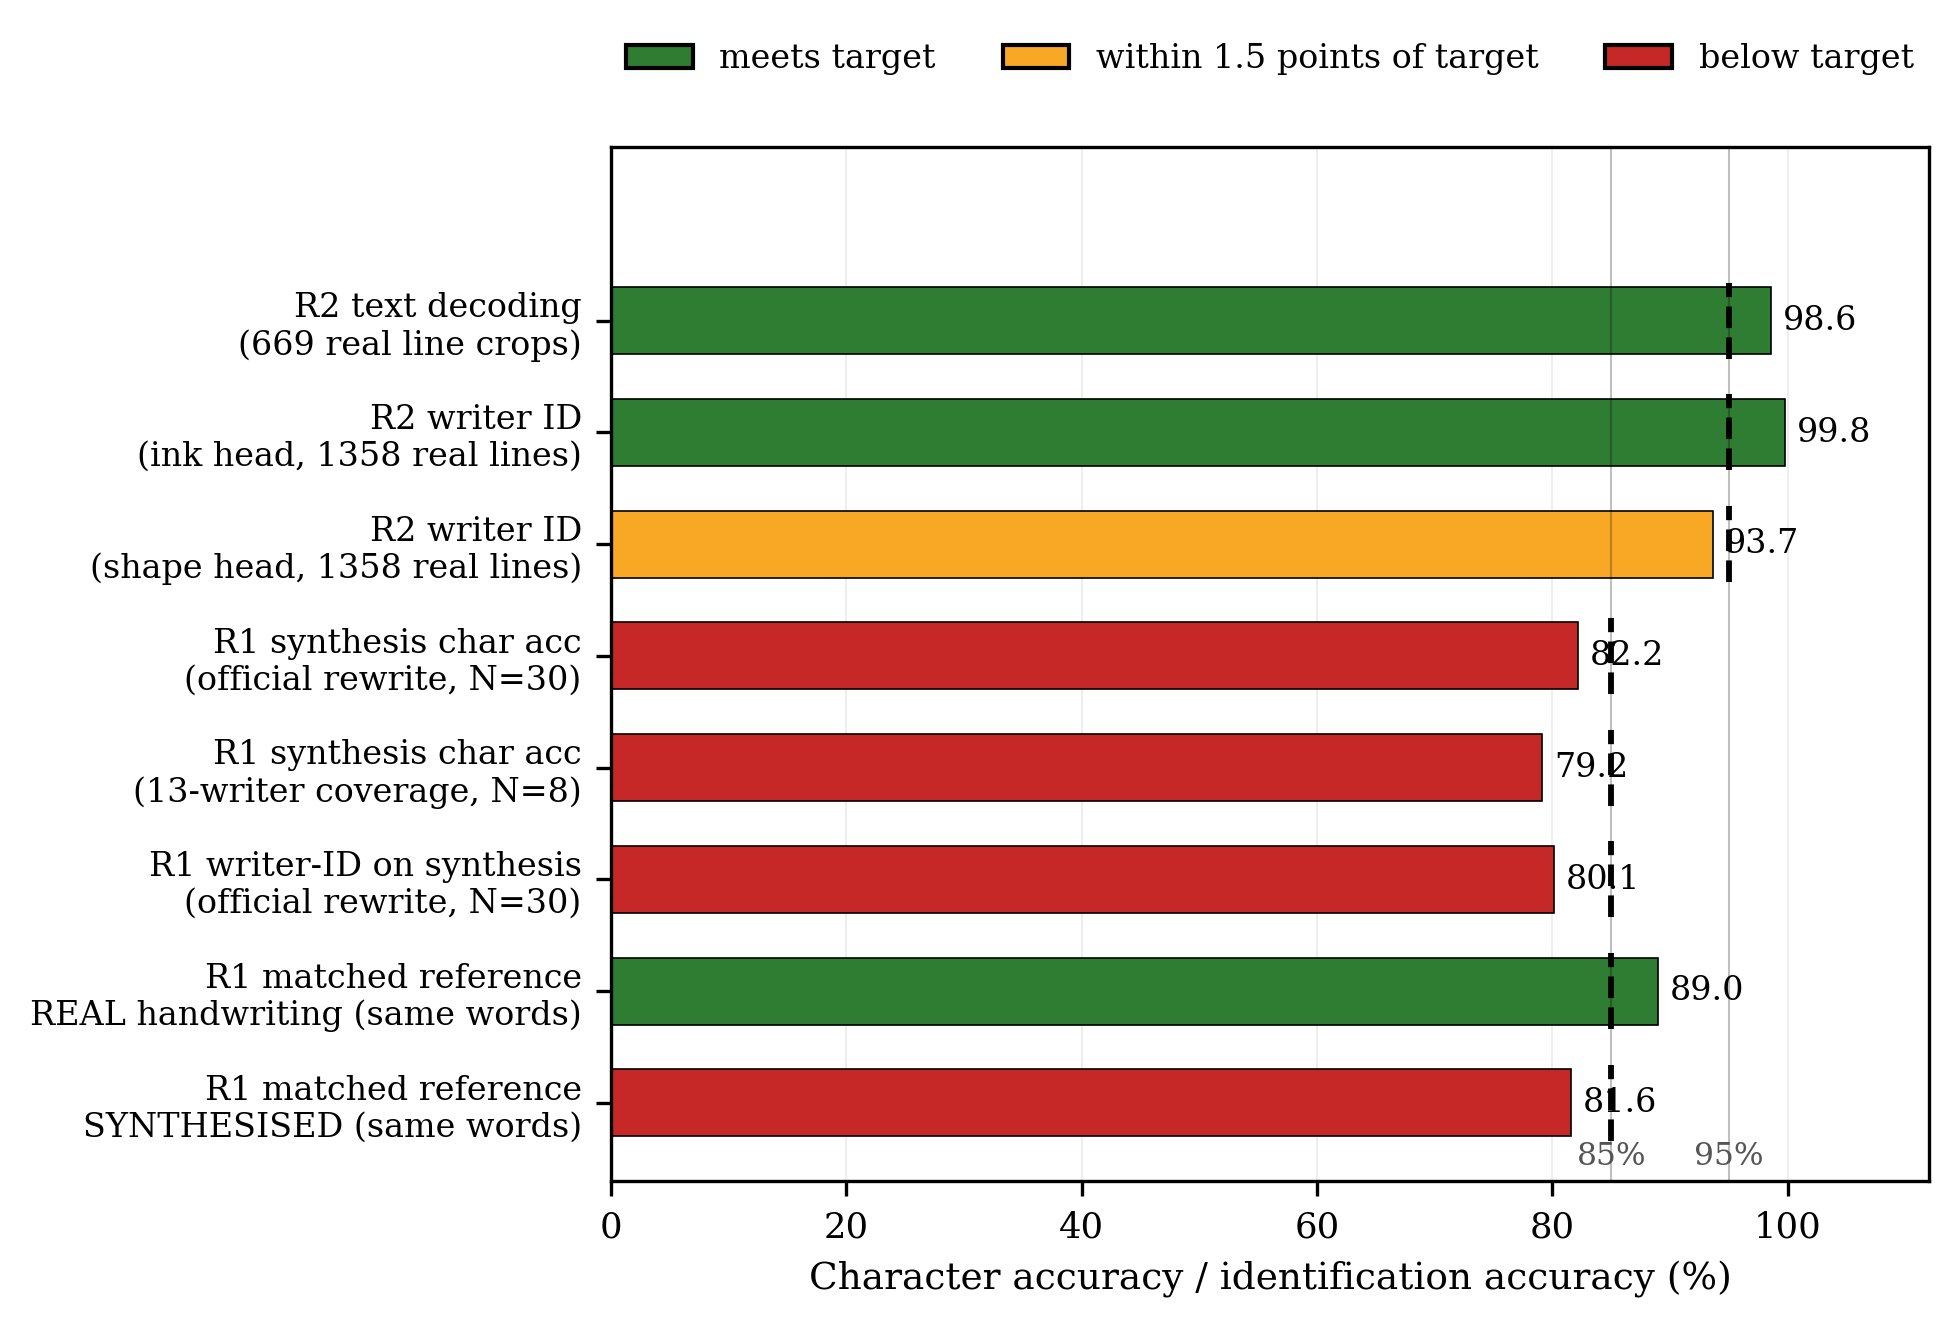
\includegraphics[width=0.85\linewidth]{Figures/res_requirements_vs_achieved.png}
\caption{Measured accuracy against the target of each requirement. Targets are marked by the dashed vertical lines at 85\% (R1) and 95\% (R2). Green bars meet the target, amber bars lie within 1.5 points of it, and red bars fall below it. The two green R1 bars are the matching comparison on genuine handwriting and the writer classifier on real lines; the red synthesis bars are the values the system actually produces.}
\label{fig:res-bars}
\end{figure}

\begin{figure}[h]
\centering
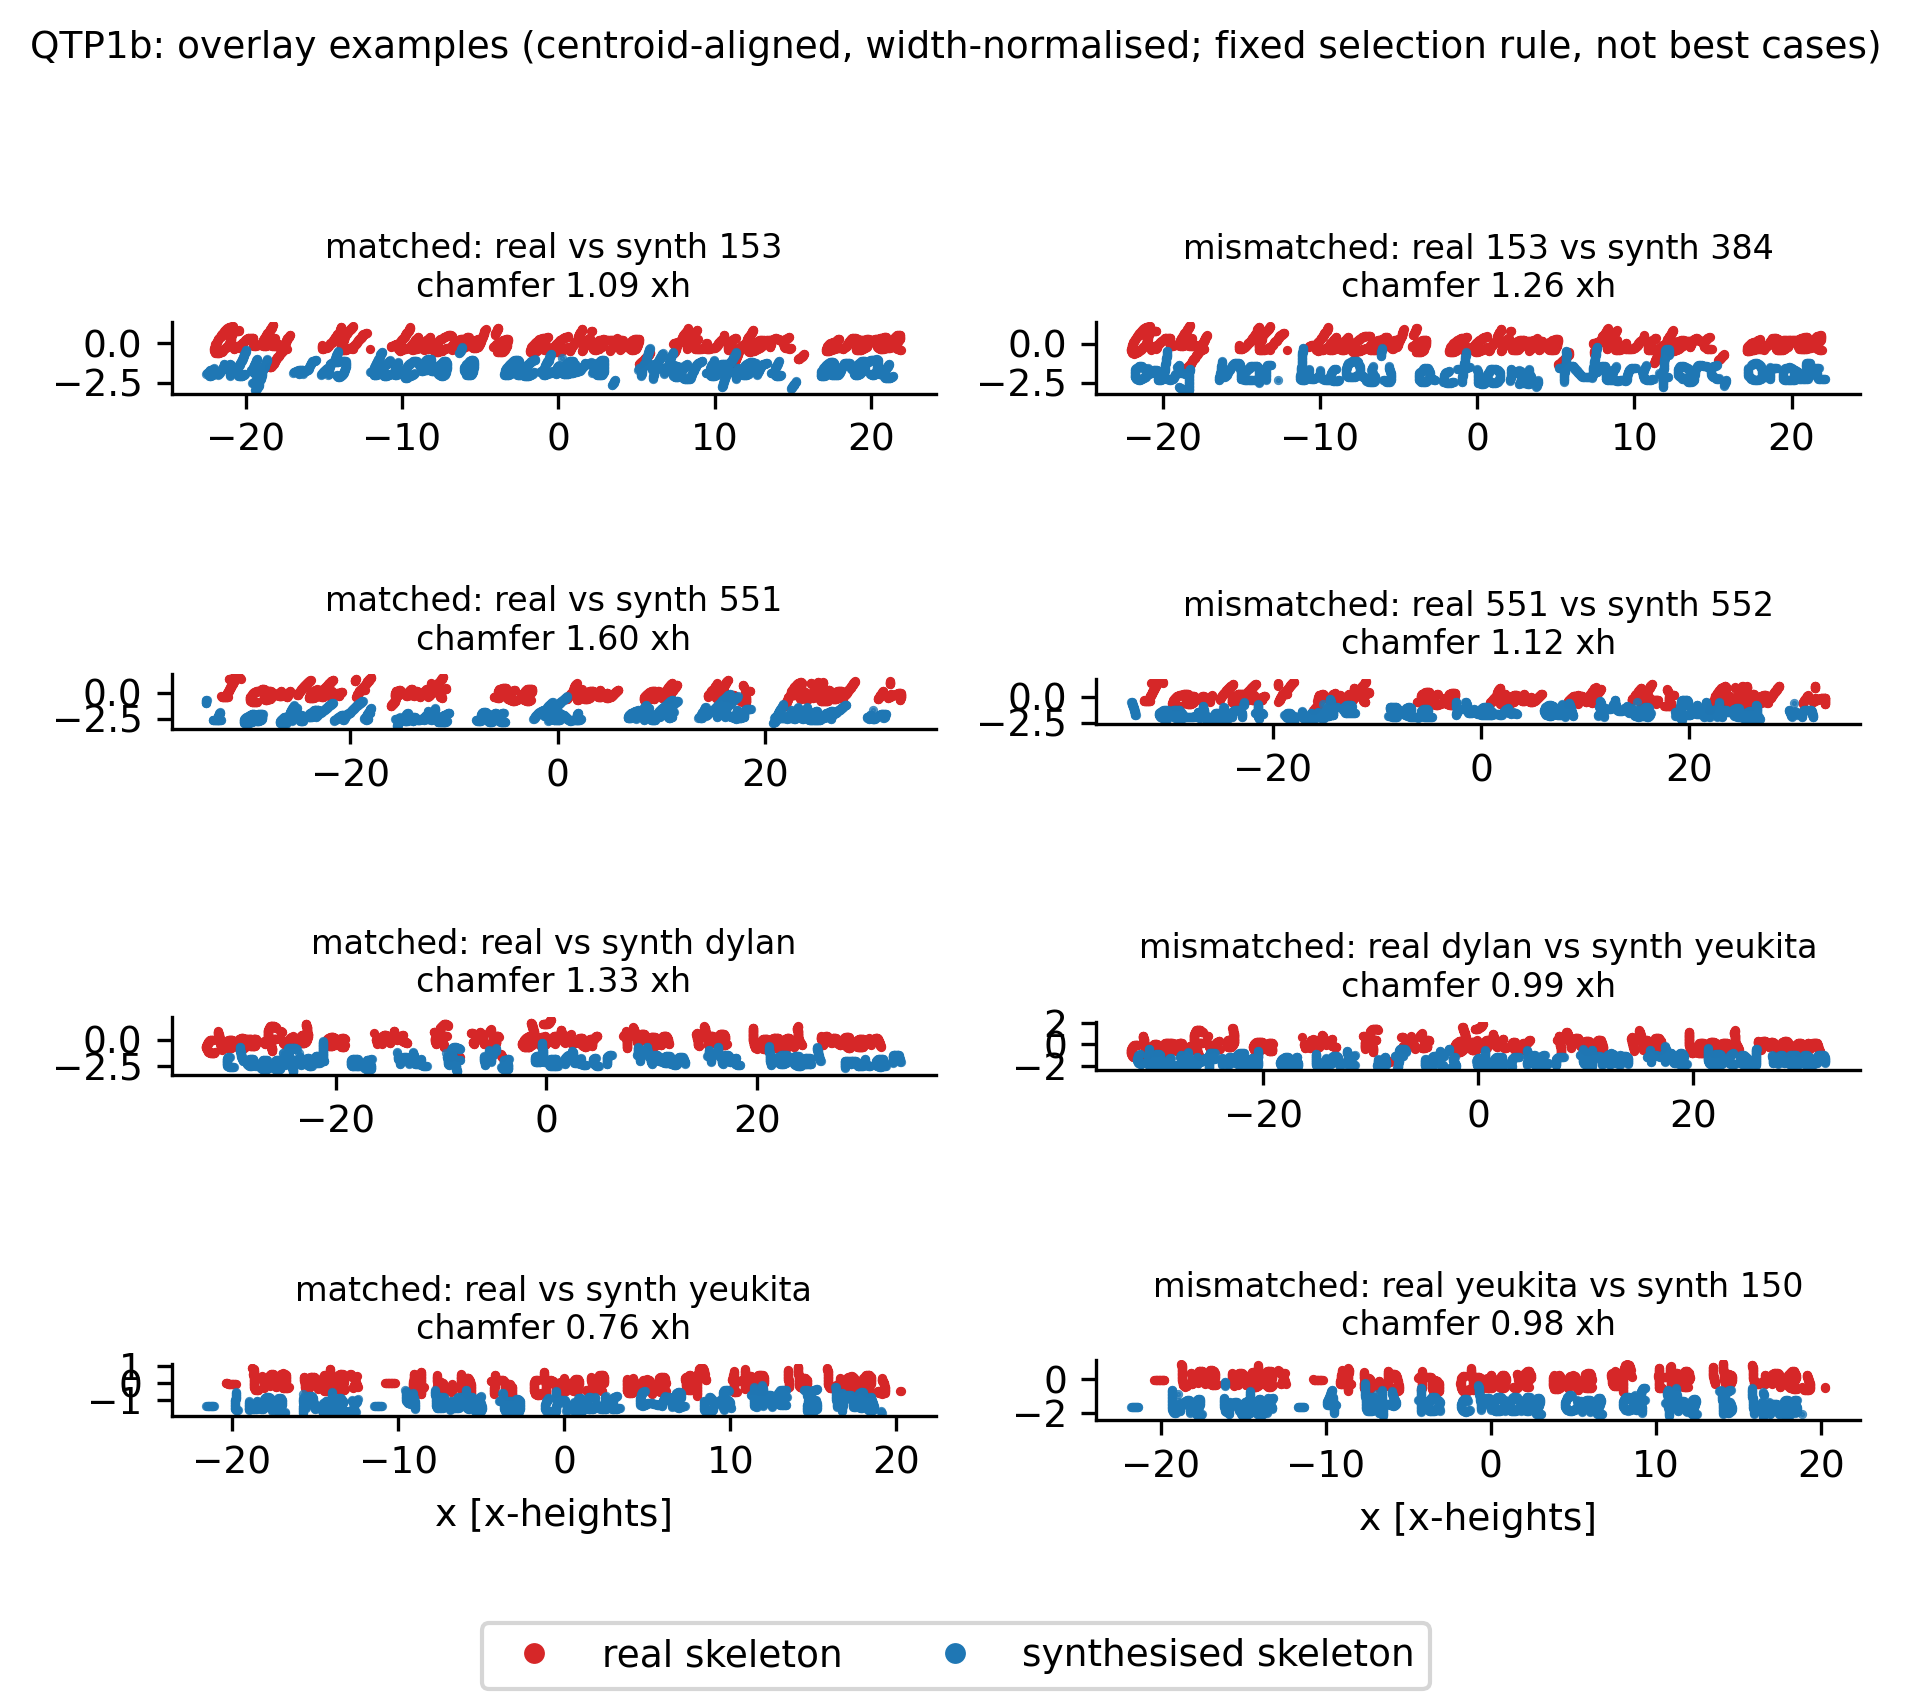
\includegraphics[width=0.85\linewidth]{Figures/qtp1_overlay_examples.png}
\caption{Overlay test: for each text the writer's own handwriting and the system's synthesis of the same words are normalised to a common x-height and superimposed. Matched pairs are visibly closer than mismatched pairs, which is what the distance ratios and the rank-1 retrieval rate of 20\% (chance 10\%) measure. The procedure that produces these overlays is given as Figure~\ref{fig:res-overlay}.}
\label{fig:res-overlay-examples}
\end{figure}


        \QualificationSection{Observations}

            The nine-feature style correlation was 0.714 on shape-only features, below the 0.85 target, with a bootstrap interval over writers of 0.612 to 0.859.
            Per feature it was highest for slant (0.996) and ascender extent (0.974) and lowest for descender extent (0.148), the ascender-to-descender ratio (0.509) and the word gap (0.605), that is for the extents below the baseline and for the spacing. The word-accuracy gap between the synthesis and real handwriting of the same words was 23.8 points.
            The overlay test gave an AUC of 0.71 against 0.5 for no writer information, and rank-1 retrieval of 20\% against a chance of 10\%.
            A partially independent checkpoint read the synthesised lines 3.7 points below the production checkpoint, 81.2\% against 84.9\% as a mean over writers, on the same 60 lines at best-of-20 (\texttt{meta.nTries\_in\_synthesis} is 20 in \texttt{qtp1c\_results.json}); the two-judge pair is therefore (84.9, 81.2) at $N=20$, and not a best-of-30 comparison.
            Against the real-ink ceiling, the production checkpoint read genuine handwriting of the same words at 89.0\% over the 70-line matched-reference set and 89.5\% over the 123 held-out lines, about 8 points above the independent judge's reading of the synthesis.
            Part of that gap is the judge and not the synthesis: on the same 123 real lines the independent checkpoint itself reads only 86.6\% against the production checkpoint's 90.2\% (both means over writers), so its own penalty on real ink is about 3.6 points.
            All of these readings cover the ten-writer subset.
            An earlier comparison measured 75.9\% before the search was introduced and 81.6\% after it.
            \NoHumanPanel


        \QualificationSection{Statistical analysis}

            By the Wilson interval of Equation~\ref{eq:res-wilson}, the official run's 82.2\% over 156 sentences has a lower bound near 75\%, so the result is below 85\% and not a sampling fluctuation.
            The style correlation is bootstrapped over writers (2000 resamples), the correct unit because the nine features are measured per writer, and the overlay AUC over 30 matched and 300 mismatched pairs.
            The two-judge comparison is paired, both checkpoints reading the same 60 synthesised lines, so the 3.7-point difference is not affected by sampling variation in the output.
            The proportion of characters a human observer would accept as matching the writer's style, which is how the proposal worded the demonstration, was not measured.

%%%%%%%%%%%%%%%%%%%%%%%%%%%%%%%%%%%%%%%%%%%%%%%%%%%%%%%%%%%%%%%%%%%%%%%%%%%%%%%%%

\medskip
    \QualificationTest{Classification of text and writer from real photographed pages (R2)}
\label{sec:res-qtp2}

        \QualificationSection{Objectives of the test or experiment}

            The test is to prove an overall accuracy of at least 95\% through the whole chain on pages never used for training, checkpoint selection or tuning.
            As the proposal does not define ``overall'', text accuracy $A_{\mathrm{c}}$ (Equation~\ref{eq:res-cacc}) and writer accuracy $A_{\mathrm{w}}$ (fraction of pages assigned to the correct writer) are reported separately and combined as
            \begin{equation}
            \label{eq:res-overall}
            A_{\mathrm{mean}}=\tfrac{1}{2}\left(A_{\mathrm{c}}+A_{\mathrm{w}}\right),\qquad A_{\mathrm{prod}}=A_{\mathrm{c}}\,A_{\mathrm{w}},
            \end{equation}
            where $A_{\mathrm{prod}}$ (both correct) is the criterion and $A_{\mathrm{mean}}$ the lenient reading.

        \QualificationSection{Equipment used}

            The capture rig and its camera photographed the pages of the five personal writers. Segmentation, recognition and writer classification then ran on the development laptop with the final server and models; the ODROID N2+ produced no figure in this test. Camera and lamp: \mustdo{camera model, resolution, mounting height, lamp type and photograph of the rig}.

        \QualificationSection{Test setup and experimental parameters}

            The line-level validation split of the personal writers leaks: a random 15\% of lines per page was held out, so lines from the same sheet and session are in both sets (52 of 123 validation lines share pages with training), and the checkpoint was selected on them.
            The fix is new pages kept aside: at least 3 per personal writer, plus the held-out form page of each of the eight database writers, photographed with the rig (about 14 pages, 350 lines). Seen lines are scored separately to quantify the leakage, and references are double-entered transcripts.

        \QualificationSection{Steps followed in the test or experiment}

            Each frozen photograph is classified through the server without intervention; line text, per-line probabilities and page-level mean probabilities are recorded, scored and summarised in a $10\times10$ confusion matrix, and the predefined paragraph is then classified live.

        \QualificationSection{Results or measurements}

            Table~\ref{tab:res-r2} lists the measured figures. Text and writer accuracy are separate, with Equation~\ref{eq:res-overall} combining them where both exist.

\begin{table}[h]
\centering
\fontsize{10}{12}\selectfont
\begin{tabularx}{\linewidth}{|>{\raggedright\arraybackslash}p{4.9cm}|>{\raggedright\arraybackslash}X|}
\hline
\textbf{Measure} & \textbf{Measured value, data set and caveat} \\
\hline
Recogniser, character accuracy & 98.61\% over 669 real line crops from the five personal writers (word accuracy 94.21\%). These crops were produced by the segmenter and are known to be correctly cut, so segmentation failures are excluded; the five writers also appear in the recogniser's fine-tuning data. \\
\hline
Recogniser, per writer & Owen is the strongest at 99.15\% and Thiya the weakest at 96.46\% character accuracy, over 75 to 206 crops each; the full breakdown is Table~\ref{tab:res-perwriter}. \\
\hline
Writer identification, ink classifier & 99.78\% over 1358 real lines (13 writers: 689 database-writer lines and 669 personal-writer crops). Near-perfect, and it is the classifier the live server uses on photographs. \\
\hline
Writer identification, shape classifier & 93.67\% over the same 1358 lines, against 83.36\% before a training fault was corrected (Section~\ref{sec:res-qtp1}). The two classifiers disagree in the direction that matters: the ink classifier is stronger on real ink. \\
\hline
Per-writer detail & Figure~\ref{fig:res-writerid}. Eight writers are at 98.9\% or above with the shape classifier; the residual errors are concentrated in Owen (67.6\%), Dylan (84.7\%) and Thiya (93.3\%). \\
\hline
Live server classification, one crop & \textbf{One} detected line, the correct writer (Owen) at \textbf{89.4\%} confidence, with the next candidate (Dylan) at 10.5\%, and a near-correct transcription (``Vloggers using fame to supfort charities is a positiwe way''). The input was a single already-segmented crop, not a whole photograph, and the call took 2.74~s end to end (\texttt{stage6\_results.json}). A single crop, reported as an illustration and not as a statistic. No whole-page run of the live classify endpoint was recorded: \mustdo{classify a full photographed page through the live server and record \texttt{lines\_detected}, the writer confidence and the transcription, so that a page-level live figure exists.} \\
\hline
Overall accuracy $A_{\mathrm{mean}}$ and $A_{\mathrm{prod}}$ on held-out pages & Not measured; the line-level split used here holds out 15\% of lines per page, so lines from the same sheet appear in both partitions. \\
\hline
\end{tabularx}
\caption{Results for qualification test 2 (13 writers; measured on the development laptop).}
\label{tab:res-r2}
\end{table}


        \QualificationSection{Observations}

            Text decoding reached 98.61\% character accuracy and 94.21\% word accuracy on correctly segmented crops, against the 95\% target, on writers represented in the recogniser's fine-tuning data; writer identification reached 99.78\% with the ink classifier over 1358 real lines from thirteen writers.
            Thiya is the weakest writer for recognition at 96.46\% character accuracy, and Owen, Dylan and Thiya the weakest for shape-based identification.
            Together the two give $A_{\mathrm{mean}}=98.6\%$ and $A_{\mathrm{prod}}=98.4\%$, both above 95\%, on a split that holds out 15\% of lines per page, so lines from the same sheet appear in both partitions.
            Both accuracies are per line and were read by the \texttt{paper\_cnn\_bilstm\_ctc\_joint\_best} text checkpoint and the \texttt{author\_classifier\_10new\_weights} ink checkpoint; the live server serves a different text checkpoint, as Section~\ref{sec:res-qtp} states.
            The one live-server run recorded was a single already-segmented crop: one detected line, the correct writer at 89.4\% confidence, 2.74~s end to end. The 98.6\% figure that belongs to this test is the character accuracy of 669 crops, not a writer confidence.

        \QualificationSection{Statistical analysis}

            With 669 line crops, 98.61\% character accuracy has a Wilson lower bound of about 97.6\%, so the text figure is above 95\% on this data set; 1358 lines at 99.78\% give a lower bound above 99\% for writer identification.
            The stronger caveat is dependence rather than sampling error: lines from one page share a writer, a pen and an illumination, so the effective sample size is nearer the page count than the line count, and the per-page interval would be much wider.
            \emph{Expected outcome on genuinely unseen pages.}
            Both rates are expected to fall, because the ink classifier is sensitive to pen, paper and illumination and the split shares pages between partitions. A defensible figure needs a page-level split with at least three held-out pages per writer, photographed through the rig.

%%%%%%%%%%%%%%%%%%%%%%%%%%%%%%%%%%%%%%%%%%%%%%%%%%%%%%%%%%%%%%%%%%%%%%%%%%%%%%%%%

\medskip
    \QualificationTest{Reproduction time per character (R3)}
\label{sec:res-qtp3}

        \QualificationSection{Objectives of the test or experiment}

            The test is to prove that a sentence of $x$ characters is reproduced within $4x$ seconds,
            \begin{equation}
            \label{eq:res-r3}
            t_{\mathrm{char}}=\frac{T_{\mathrm{syn}}+T_{\mathrm{write}}}{x}\le 4\ \mathrm{s},
            \end{equation}
            where $T_{\mathrm{syn}}$ is the synthesis time and $T_{\mathrm{write}}$ the time from first to last motion.
            As the proposal does not say whether synthesis counts, both variants are reported; calibration is a one-off step, reported separately.

        \QualificationSection{Equipment used}

            The development laptop with the server, and logged time stamps around synthesis. The gantry and a stopwatch were to have given the writing time, but the gantry was not driven, because its bring-up was not completed, so the motion time is a model and not a measurement.

        \QualificationSection{Test setup and experimental parameters}

            The run actually made, recorded in \texttt{qtp\_data/qtp3\_results.json}, used tries $N\in\{1,3,14,30\}$ and five sentences of 22, 40, 58, 83 and 119 characters, with 3, 3, 3 and 2 repetitions for the four values of $N$ respectively (20 cells, 56 syntheses), writer 153 throughout, plus a writer-dependence extra at 58 characters and $N=14$; the writing time is the generator's model for every cell, not a stopwatch reading.
            The protocol as originally written had prescribed $N\in\{1,3,6,14,30\}$, sentences of 10, 20, 40 and 80 characters and 5 repetitions (100 syntheses), with the writing time measured for the 20 jobs at $N=14$; that plan was not the one executed, and the results below are reported against the run that was.
            Only figures measured on the ODROID N2+ itself count; laptop figures are indicative.

        \QualificationSection{Steps followed in the test or experiment}

            After one calibration, each job is synthesised, sent and timed by log and stopwatch, $t_{\mathrm{char}}$ is computed from Equation~\ref{eq:res-r3}, and any stall is kept as a failed run.

        \QualificationSection{Results or measurements}

            Table~\ref{tab:res-r3} and Figure~\ref{fig:res-r3} give the measured figures: a synthesis term that grows with the number of candidates and a writing term that does not.

\begin{table}[h]
\centering
\fontsize{9.5}{11.5}\selectfont
\begin{tabularx}{\linewidth}{|>{\raggedright\arraybackslash}p{4.6cm}|>{\raggedright\arraybackslash}X|}
\hline
\textbf{Measure} & \textbf{Measured value, data set and caveat} \\
\hline
Synthesis time per character, best-of-1 to best-of-30 & Repeated over sentences of 22 to 119 characters and 2 to 3 repetitions per cell, on the development laptop. At best-of-1 the synthesis costs about 0.4 to 0.7~s per character; at best-of-14 about 0.9 to 1.8~s per character; at best-of-30 about 1.8 to 3.4~s per character. \\
\hline
G-code generation & 0.006 to 0.014~s per sentence, i.e.\ negligible at any sentence length. \\
\hline
Preview rendering and read-back & About 0.02 to 0.05~s and 0.6 to 0.8~s per sentence respectively; both are small beside the synthesis term. \\
\hline
Physical writing time, from the generator's own model & 88.7~s for a 22-character sentence and 154.4~s for a 58-character sentence, i.e.\ about 2.7 to 4.0~s per character, against the 4~s limit \emph{for the writing alone}. \\
\hline
Total per character at best-of-14 & Figure~\ref{fig:res-r3}: synthesis contributes about 1.0 to 1.8~s and writing about 2.7 to 4.0~s, so the total lies between about 4 and 6~s per character and straddles the limit. \\
\hline
Live server measurement, four-character word, best-of-6 & 64.3~s from request to rendered preview, i.e.\ 16.1~s per character. A very short sentence is the worst case because the per-job costs (model loading, segmentation of the uploaded image) are amortised over only four characters. \\
\hline
Physical writing time measured on the gantry & Not measured; the gantry bring-up was not completed, so no drawn job was timed. The figures above are the generator's model, not observations. \\
\hline
Timing on the ODROID N2+ & Not measured. \\
\hline
\end{tabularx}
\caption{Results for qualification test 3 (development laptop; the writing figures are model values, not measurements).}
\label{tab:res-r3}
\end{table}

\begin{figure}[h]
\centering
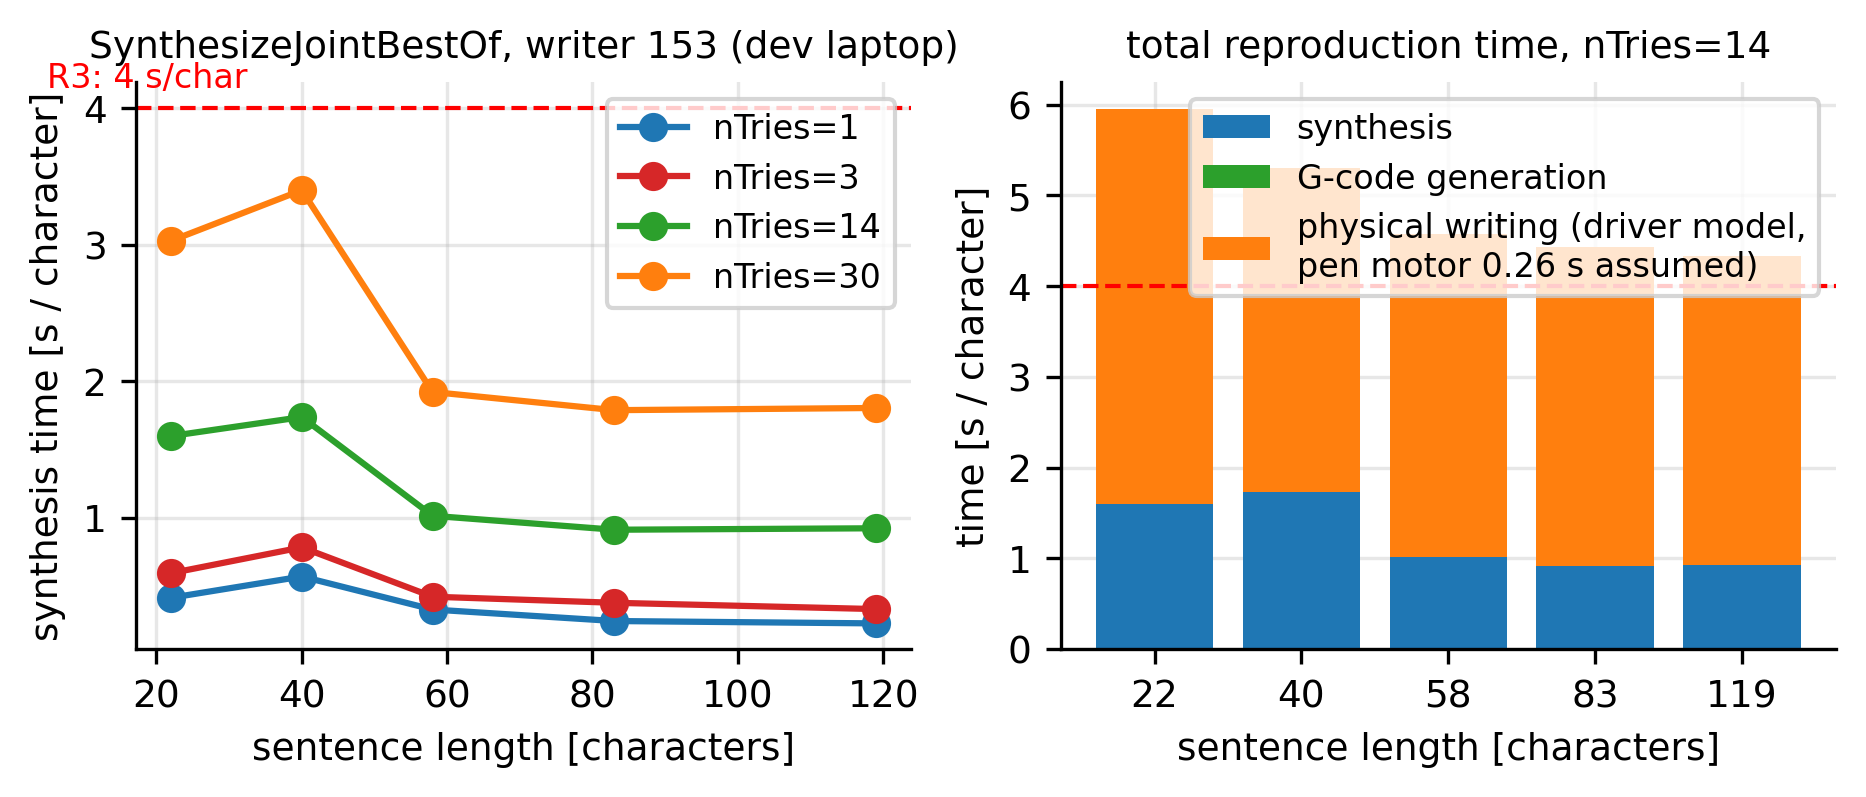
\includegraphics[width=0.85\linewidth]{Figures/qtp3_timing_breakdown.png}
\caption{Reproduction time against the 4~s per character limit of R3. Left: synthesis time per character against sentence length for four values of the number of candidates. At best-of-1 and best-of-3 the synthesis alone is comfortably inside the limit; at best-of-30 it approaches and crosses it. Right: total time per character at best-of-14, decomposed into synthesis, G-code generation and the physical writing time predicted by the generator's model. The writing term, not the synthesis term, is the larger contributor and is what pushes the total past the limit.}
\label{fig:res-r3}
\end{figure}

        \QualificationSection{Observations}

            The synthesis cost stayed well under 1~s per character up to best-of-3 and grew in proportion to the number of candidates, from about 0.4 to 0.7~s per character at best-of-1 to about 1.8 to 3.4~s at best-of-30.
            The generator's model gives 2.7 to 4.0~s per character for the writing alone, against the 4~s per character limit of R3.
            The four-character word at best-of-6 gave 16.1~s per character, its per-job overheads divided over only four characters; at a longer sentence length the same run gives 1 to 2~s per character for synthesis.
            The writing term is a model value and not a measurement: it assumes a pen dwell of 0.26~s per stroke, and no drawn job was timed on the gantry.

        \QualificationSection{Statistical analysis}

            Each cell is the mean of two or three repetitions, and the table quotes a range, because for short sentences the variation between repetitions was of the same order as that between configurations.
            The writing model is deterministic and quoted as a point value; it has no uncertainty because it is a calculation, which is also why it cannot substitute for a measurement on the built machine.
            The proposal does not state whether synthesis counts towards the limit, so Table~\ref{tab:res-r3} reports both readings.

%%%%%%%%%%%%%%%%%%%%%%%%%%%%%%%%%%%%%%%%%%%%%%%%%%%%%%%%%%%%%%%%%%%%%%%%%%%%%%%%%

\medskip
    \QualificationTest{Classification time (R4)}
\label{sec:res-qtp4}

        \QualificationSection{Objectives of the test or experiment}

            The test is to prove that the time from instruction to displayed text and writer satisfies
            \begin{equation}
            \label{eq:res-r4}
            T_{\mathrm{cls}}\le 2+0.025\,x\ \text{seconds},
            \end{equation}
            where $x$ is the number of handwritten characters; the stage times identify any shortfall.

        \QualificationSection{Equipment used}

            The rig, the development laptop with the final server, and a logging wrapper (monotonic clock) around each stage. The ODROID N2+ was not timed, so the figures below are laptop figures and the board is expected to be slower. The interface does not display classification time.

        \QualificationSection{Test setup and experimental parameters}

            Pages with $x=40$, about 200 and about 1000, each run 10 times; the budgets are 3.0, 7.0 and 27.0~s.
            Stages: capture, conditioning and segmentation, recognition per line, writer classification, display; the segmentation profile is repeated on the ODROID N2+.

        \QualificationSection{Steps followed in the test or experiment}

            The clocks start at the instruction, stage times and the total are logged, $x$ is counted from the transcript and Equation~\ref{eq:res-r4} is evaluated.

        \QualificationSection{Results or measurements}

            Table~\ref{tab:res-r4} lists the measured figures.

\begin{table}[h]
\centering
\fontsize{10}{12}\selectfont
\begin{tabularx}{\linewidth}{|>{\raggedright\arraybackslash}p{4.9cm}|>{\raggedright\arraybackslash}X|}
\hline
\textbf{Measure} & \textbf{Measured value, data set and caveat} \\
\hline
Recognition time per character & 8.86~ms per character and 353~ms per line, averaged over 669 real line crops (236.2~s of inference in total). This meets the 25~ms per character allowance with a margin of about 2.8 times. Measured on the development laptop with the model already loaded. \\
\hline
Writer classification time & A single crop classified through the live server took 2.74~s end to end, which includes segmentation of the uploaded image, the ink writer classifier and text recognition of the line. \\
\hline
Total classification time, one page & \textbf{Measured.} 13 photographed pages, 3 repeats each (\texttt{qtp\_data/qtp4\_results.json}): page means of \textbf{40.3 to 100.1~s} from file read to displayed writer and text, against per-page budgets of 26.4 to 43.9~s from Equation~\ref{eq:res-r4} for $x=976$ to 1677 characters. The ratio of total to requirement is \textbf{1.15 to 2.98}, so every page exceeded its budget, the best by 15\% and the worst by a factor of three. Individual repeats ran from 40.2 to 103.4~s. Stage breakdown on the same run: file I/O 0.35 to 0.97~s, segmentation 24.8 to 69.1~s, recognition 5.7 to 13.8~ms per character, writer classification 4.6 to 10.3~ms per character. All 13 pages were from two writers (Yeukita and Dylan) and are the harness pages, not a thirteen-writer sample. Measured on the development laptop. \\
\hline
Page segmentation time & 24.8 to 69.1~s per page (first repeat of each of the 13 pages; 24.7 to 72.4~s over all 39 repeats) for $2448\times3264$ photographs in pure Python on the laptop, against the roughly 2~s that the equation allows for capture and conditioning. \textbf{Attribution:} the stored field is \texttt{stage1\_processpage\_s}, so these are timings of \texttt{SegmentPage.ProcessPage}, the \emph{retired} segmenter, and \emph{not} of the deployed \texttt{SegmentLean.py}. No timing of the deployed module exists: \mustdo{time \texttt{SegmentLean.py} on the same 13 pages with the same 3 repeats, so that the segmentation term of R4 refers to the module the system actually ships.} Two routines reimplemented in C99 reduced the retired segmenter by 25\% to 32\% end to end, but they were not deployed. \\
\hline
Timing on the ODROID N2+ & Not measured. \\
\hline
\end{tabularx}
\caption{Results for qualification test 4 (development laptop).}
\label{tab:res-r4}
\end{table}

        \QualificationSection{Observations}

            Recognition ran at 8.86~ms per character, about a third of the 25~ms allowance.
            Segmentation of one photograph took 24.8 to 69.1~s, that is 12 to 35 times the two seconds the equation allows for capture and conditioning; this cost is per page and does not vary with $x$, which appears only in the recognition term of Equation~\ref{eq:res-r4}.
            These segmentation times are readings of the field \texttt{stage1\_processpage\_s}, which times \texttt{SegmentPage.ProcessPage}, the retired segmenter. The deployed \texttt{SegmentLean.py} was not timed.
            Total time for one page was 40.3 to 100.1~s against budgets of 26.4 to 43.9~s, a ratio of 1.15 to 2.98 over the 13 pages measured.
            A single already-segmented crop was classified through the live server in 2.74~s end to end, returning one detected line and the correct writer at 89.4\% confidence.

        \QualificationSection{Statistical analysis}

            The recognition timing is an average over 669 crops; the per-character figure is total inference time divided by total characters, so it is a throughput measure rather than a per-line latency.
            The page-level timing is 13 pages $\times$ 3 repeats, reported as the per-page mean with the range over pages; ten of the thirteen pages had their three repeats within 8\% of each other, but three spread by 17\%, 52\% and 83\% between fastest and slowest repeat, so the upper end of the range carries the larger uncertainty.
            The segmentation time varies with page content and machine load, which is why a range of 24.8 to 69.1~s is reported; the lower end was obtained on an idle machine.
            The whole segmentation range belongs to the retired \texttt{SegmentPage.ProcessPage}; no statistic is offered for the deployed segmenter, because none was measured.
            These numbers indicate moving segmentation to compiled code or processing the page incrementally, as the C99 experiment suggests a saving of about a quarter to a third without changing the algorithm.
            \emph{Expected outcome.}
            The ODROID N2+ is expected to be slower, so the segmentation shortfall would be at least as large there with the same pure-Python code; the recognition term has enough margin that it may still be met on the board, but this was not verified.

%%%%%%%%%%%%%%%%%%%%%%%%%%%%%%%%%%%%%%%%%%%%%%%%%%%%%%%%%%%%%%%%%%%%%%%%%%%%%%%%%

\medskip
    \QualificationTest{Absolute positional accuracy of the gantry (R5)}
\label{sec:res-qtp5}

        \QualificationSection{Objectives of the test or experiment}

            The test is to prove that the absolute positional error of drawn marks is at most 0.5~mm and that a word written twice coincides within that tolerance.
            Software contributions (quantisation, calibration) and hardware contributions (mechanics, homing repeatability, pen compliance) are separated.

        \QualificationSection{Equipment used}

            The gantry with pen and paper, a flat-bed scanner (600 dots per inch, 0.042~mm per pixel), a steel ruler or vernier calipers (0.02~mm) and a printed calibration sheet with a 10~mm grid of crosses.

        \QualificationSection{Test setup and experimental parameters}

            Software part (offline): the step is $1/80=12.5~\mu$m, the quantisation error per axis at most $6.25~\mu$m and the combined worst case $8.8~\mu$m (derived).
            Hardware part, prescribed but not executed: at least 40 crosses drawn 5 times after fresh calibrations, the paper fixed against registration stops, and the same word written twice.
            The quantity to be measured is the absolute error $e_i$ of each cross against its commanded centre, reported as mean, maximum and 95th percentile and accompanied by a combined standard uncertainty over the scanner scale, the registration of the sheet and the location of a cross centre; both are defined in Appendix~\ref{sec:app-met} as Equations~\ref{eq:res-r5} and~\ref{eq:res-unc}, following the Guide to the Expression of Uncertainty in Measurement~\cite[Clause~5]{jcgm2008}.
            Table~\ref{tab:res-sheet} is the sheet on which those measurements were to be recorded, one row per cross and repetition. Because no mark was ever drawn, neither equation was evaluated and the sheet was never filled in; it is reproduced blank to define the measurement that is missing.


        \QualificationSection{Steps followed in the test or experiment}

            The protocol has five steps: (1) calibrate and verify the direction pin on both axes, the pin having to be seen to change level on reversal, and record the calibrated steps per millimetre; (2) fix the sheet against the stops, draw the grid and scan it with the ruler; (3) locate the cross centres with sub-pixel image analysis, compute the error of Equation~\ref{eq:res-r5} and enter each row in Table~\ref{tab:res-sheet}; (4) repeat 5 times and write the same word twice on one sheet for the overlay; (5) estimate the uncertainty of Equation~\ref{eq:res-unc}.
            Repeatability is defined as the radius of scatter of the 5 repeats of one cross about its centroid.
            Only step (1) was attempted, and it did not complete: the X-axis calibration drove to the first end-stop but the direction pin was not observed to change level on reversal. Steps (2) to (5) were therefore never performed, no grid was drawn and no overlay of a word written twice was produced, so this test was not carried out.

        \QualificationSection{Results or measurements}

            The only quantities that exist are derived from the mechanical configuration, not measured on a drawn mark.
            The X and Y axes are belt-driven: a 200-step motor, sixteen microsteps per step and a 40~mm advance per revolution give
            \begin{equation}
            \label{eq:res-step}
            \Delta s=\frac{40\ \mathrm{mm}}{200\times16}=12.5\ \mu\mathrm{m}\ \text{per step},
            \end{equation}
            so by Equation~\ref{eq:res-step} the quantisation error of one axis is at most $6.25~\mu$m and the worst case over both axes $\sqrt{2}\times6.25=8.8~\mu$m.
            Two different margins against the 0.5~mm limit follow from this, and they are quoted for two different quantities; they are not in conflict.
            The \emph{step pitch} is 12.5~\textmu m, which is $0.5/0.0125=40$ times finer than the limit; the \emph{combined worst-case quantisation error} is 8.8~\textmu m, which is $0.5/0.0088\approx57$ times finer than it.
            Where this chapter says 40 times it means the step pitch, and where it says 57 times it means the combined two-axis quantisation error.
            Neither figure is a measurement of a drawn mark.
            During bring-up the X-axis calibration drove to the first end-stop, but the direction pin did not change level on reversal; the fault was not resolved and no grid was drawn, so there is no overlay of a word written twice and the measurement of $e_i$ remains \nym{}.

        \QualificationSection{Observations}

            No positional measurement exists.
            The one hardware observation is the direction-pin fault: the X-axis calibration drove to the first end-stop and the direction pin was not observed to change level on reversal. No grid was drawn, so the test was not carried out. The derived step pitch is 12.5~\textmu m per step and the derived combined two-axis quantisation error 8.8~\textmu m, against a tolerance of 0.5~mm.

        \QualificationSection{Statistical analysis}

            No statistics can be reported for a measurement that was not taken.
            \emph{Expected outcome.}
            The error is expected to be dominated by belt stretch, backlash, home-switch repeatability and pen compliance, none of which was measured.
            Published handwriting gantries report about 0.3~mm absolute error~\cite{huang2024}, a margin of 0.2~mm against this limit; whether this machine achieves that cannot be stated.
            A pass requires the maximum $e_i$ over at least 200 drawn marks to be at most 0.5~mm, by scanning the sheet at 600~dots per inch.

%%%%%%%%%%%%%%%%%%%%%%%%%%%%%%%%%%%%%%%%%%%%%%%%%%%%%%%%%%%%%%%%%%%%%%%%%%%%%%%%%

\medskip
    \QualificationTest{Multi-writer storage (R6)}
\label{sec:res-qtp6}

        \QualificationSection{Objectives of the test or experiment}

            The test is to prove that at least 10 writing styles are stored permanently and that any can be selected at random for reproduction.

        \QualificationSection{Equipment used}

            The development laptop with the server and a browser. The gantry was not used, because the reproduction half of this test was not carried out.

        \QualificationSection{Test setup and experimental parameters}

            The eight database and five personal writers; file counts and sizes; persistence by restarting the server and power-cycling the board; 3 writers drawn with a fixed seed.

        \QualificationSection{Steps followed in the test or experiment}

            The listed writers are compared with the stored files, the list is re-read after restart and power cycle, and a short sentence is written in each of the 3 drawn styles.

        \QualificationSection{Results or measurements}

            The live server listed thirteen writers through its author-list endpoint in 70~ms, from thirteen stored style profiles; the requirement names ten.
            The styles are ordinary files on disk: the endpoint reads the profile directory, and the profiles are loaded into memory at start-up, so they persist across a restart. The profile and weight-file sizes are in the technical documentation, and Figure~\ref{fig:res-storage} shows the storage check.


        \QualificationSection{Observations}

            The list contained thirteen entries against a requirement of ten, and the endpoint answered in 70~ms.
            The five personal writers are stored in the same format as the eight database writers, so the storage mechanism does not distinguish scanned pages from photographed ones.
            A writer was not selected at random and written on paper, so the reproduction part of the proposal's demonstration was not carried out.

        \QualificationSection{Statistical analysis}

            This is a count against a threshold, so no statistical analysis is appropriate; the figure of thirteen is exact, not a sample estimate.
            Persistence follows from the profiles being files rather than in-memory state, and is observed each time the server re-lists them; a power-cycle test of the board was not performed, because the board was not deployed.

%%%%%%%%%%%%%%%%%%%%%%%%%%%%%%%%%%%%%%%%%%%%%%%%%%%%%%%%%%%%%%%%%%%%%%%%%%%%%%%%%

\subsubsection*{Field condition checks (FC1 and FC2)}
\label{sec:res-fc}

Neither field condition was measured.
\textbf{FC1:} a lux meter at the page plane records five points (centre and corners of an A4 page); the condition is met if all lie between 400 and 1000~lux, and qualification test 2 is repeated on the same pages at about 200, 700 and 1200~lux.
Illuminance: \nym{}; the flat-field correction and local thresholding should limit degradation within the range, with larger degradation below 400~lux.
\textbf{FC2:} a spirit level or inclinometer on both axes (tilt below $0.5^\circ$) and a logging accelerometer on the frame during a standard job, with the repeat error of qualification test 5 at rest and with a lightly tapped bench.
Tilt and vibration: \nym{}.

\newpage

\section{Discussion}
\label{sec:discussion}

\subsection{Critical evaluation of the design} % REQUIRED HEADING

This subsection interprets the results of Section~\ref{sec:results}, evaluates the design choices in hindsight and identifies what must change before the requirements can be considered proven.
\label{sec:dis-critical}

Two limitations determine every conclusion below: the measurements were taken on a development laptop and not on the ODROID N2+, and the evidence on synthesis quality is partly circular, because the classifier that selects the best of $N$ candidates belongs to the same family as the one that reports the score.
Where a figure is affected by either limitation, this is stated with the figure.

    \subsubsection{Interpretation of results}
    \label{sec:dis-interp}

        \textbf{R2, classification: the strongest part of the system.}
        Text decoding reached 98.61\% character accuracy and 94.21\% word accuracy over 669 real line crops, and writer identification 99.78\% over 1358 real lines from thirteen writers with the ink classifier.
        Both exceed the 95\% target on this evidence, and the lower bound of the character figure is about 97.6\%.
        Two qualifications do not show in the numbers.
        First, the 98.61\% is measured on crops known to be correctly cut, because any page whose crop count disagreed with the label count was excluded; it therefore measures recognition given correct segmentation and says nothing about pages where segmentation fails.
        Second, the five writers scored are also represented in the recogniser's fine-tuning data, so the split favours the system.
        Honestly stated, recognition and identification meet their target on correctly segmented, in-distribution input, and the end-to-end page-to-text accuracy is bounded above by these figures rather than equal to them.
        The gap between character and word accuracy carries information: one wrong character spoils a whole word, so the residual error sits in a minority of words rather than spread thinly.

        \textbf{The writer classifier that is used for real ink is not the one that judges synthesis.}
        The ink classifier reached 99.78\% on real lines and the shape classifier 93.67\%.
        That ordering is the opposite of what the synthesis path needs, because the ink classifier depends on stroke thickness and ink density, which a constant-width plotter cannot reproduce: on the system's own drawn output the ink classifier falls to 28\%, close to chance for thirteen writers, while the shape classifier reaches 89.7\%.
        Both are therefore necessary: one is the right instrument for reading a photograph, the other for judging a drawing.

        \textbf{A training fault, not an intrinsic difficulty, explained the hardest writer pair.}
        Before this work the shape classifier assigned 118 of one writer's 148 real lines to a single other writer, which read as two intrinsically similar hands.
        The measurement shows otherwise: training the same architecture end-to-end, instead of freezing the backbone at the recogniser's features and fitting only the classification head, raised the shape classifier from 83.4\% to 93.7\% overall and that writer from 18.9\% to 67.6\%.
        A recogniser's features are trained to be \emph{invariant} between writers, so a classifier restricted to them can separate only writers whose recognition features already differ.
        The residual is still 48 of 148 lines sent to the same neighbour, so a smaller genuine effect probably remains on top of the fault; this is unresolved and listed as an unsolved problem.
        The lesson is that reusing a recogniser's backbone saves training data, but it must be fine-tuned rather than frozen whenever the new task is to detect the variation the backbone was trained to ignore.

        \textbf{R1, representation fidelity: close, and the shortfall is in the right place to be fixable.}
        Synthesised text was read at 82.2\% character accuracy over thirteen writers, against the 85\% target, and at 79.2\% in a wider coverage run.
        The matching comparison is more informative: on identical sentences the writers' genuine handwriting was read at 89.0\% and the synthesis at 81.6\%.
        The synthesis loses 7.4 percentage points of character accuracy but 23.8 points of word accuracy, and that asymmetry localises the defect.
        Individual letterforms survive the transfer, as expected because the synthesiser draws the writer's own traced glyph paths; the spacing structure does not, so words are drawn with boundaries the recogniser reads differently.
        The measured feature deviations agree: synthesised lines have ascenders about 0.4 to 0.6 x-height units shorter than the writer's real lines, word spaces about 0.5 units narrower, and connectedness lower.
        The defect is thus a few measurable, correctable quantities rather than a failure of the method, which is why R1 is partially met rather than not met.
        A recogniser checkpoint that took no part in the search read the same lines 3.7 points below the production checkpoint, so the selection raises legibility only slightly and the result is not an artefact of the search.

        \textbf{The stylistic-correlation target is not verified, and writer identification is a weak proxy for it.}
        The proposal asks for 85\% stylistic correlation; what was measured is writer-identification accuracy, a different question, because a synthesis could be identifiable as the right writer while still differing visibly from that writer's hand.
        Worse, the writer-identification figures on synthesised text (80.1\% in the official run, 89.7\% in the coverage run) come from a classifier that also selects the candidates, so a best-of-$N$ search necessarily raises the score it is judged by, and only the figures computed outside the search can be trusted.
        The nine-feature geometric correlation gave 0.714 against the 0.85 target, so the style term of R1 is not met on that measure, the shortfall being in descender extent, the ascender-to-descender ratio and word spacing rather than in slant or ascender extent.
        The overlay test gave an AUC~\cite[p.~868]{fawcett2006} of about 0.71, against 0.5 for an output carrying no writer information, which indicates real but limited fidelity.
        A human panel or an independent classifier is required before the 85\% stylistic target can be claimed, and this was not carried out.

        \textbf{The synthesis is recognised as the correct writer much better than the system draws that writer.}
        The same shape classifier identifies 93.7\% of real lines but only 89.7\% of drawn lines in the coverage run, and only 67.6\% of one writer's real lines while identifying 100\% of that writer's drawn lines.
        A judge that recognises the machine's output more reliably than the human's hand is measuring agreement with the synthesiser rather than fidelity to the author, which is the most important caveat on every writer-identification figure measured on synthesised text.

        \textbf{R3, reproduction time: the failure is the search, not the drawing.}
        A four-character word at $N=6$ took 64.3~s, or 16.1~s per character, four times the limit.
        The coverage run confirms that the cost scales with the number of candidates, because every candidate is rendered, read by the recogniser and scored by the writer classifier.
        The physical drawing time was never measured, so the requirement cannot be decomposed, and it would be wrong to conclude that the gantry is slow: the evidence points at the selection procedure, which embeds two network passes in its inner loop and pays for the quality it delivers.
        The proposal does not state whether the synthesis time counts towards the limit; under the reading that only the physical writing counts, the generator's model value of 2.7 to 4.0~s per character sits at the 4~s limit, so the requirement is recorded as not met on the conservative reading that the total counts.

        \textbf{R4, classification time: recognition passes, segmentation fails badly.}
        Recognition ran at 8.86~ms per character against the 25~ms allowance, a margin of about 2.8 times, so the neural component is not the problem.
        Page segmentation took 35 to 57~s against the roughly 2~s the equation allows for capture and conditioning, a shortfall of more than an order of magnitude.
        Since $x$ appears only in the recognition term, a longer page does not buy proportionally more time, so the segmenter's per-page cost cannot be amortised.
        The profile shows the cause: line grouping and the chain search dominate, at about 70\% of the time, and are written in pure Python.
        Moving two inner routines to C reduced the total by 25\% to 32\%, but the grouping still dominates: accelerating the wrong part of a program cannot fix it.

        \textbf{R5, positional accuracy, and the field conditions: no conclusion is possible.}
        The derived step resolution of 12.5~$\mu$m shows only that the command quantisation is 40 times finer than the tolerance, so the error must come from the mechanics and from open-loop effects.
        No drawn mark was scanned, because the direction-pin fault prevented controlled motion in both directions, so the requirement is unassessed rather than failed.
        The same holds for the two field conditions, neither of which was measured; the illumination figure is the more consequential omission, because the conditioning stage was designed to tolerate uneven lighting and that claim is untested.

        \textbf{Requirements met.}
        The storage half of R6 is met: thirteen styles are stored as files and the live server lists all of them, against a minimum of ten, returning the list in 70~ms. The reproduction half is not: the proposal's demonstration asks for a writer to be chosen at random and the text written on paper in that style, and that was never carried out.
        R2 is met for writer identification on real handwriting and for recognition on correctly segmented in-distribution crops, but not demonstrated for the complete page-to-text chain.
        R1 is close but not met, R3 and R4 are not met, and R5 and both field conditions are unassessed.

        \textbf{Where this system sits against published work.}
        Table~\ref{tab:dis-compare} places the measured figures of Section~\ref{sec:results} beside the published systems surveyed in Section~\ref{sec:literature}.
        The comparison is not like for like and is not offered as one: every published row was obtained on a public benchmark with a full research pipeline behind it, while the rows for this project were measured on thirteen writers, five of them photographed for this project, on a system that must also synthesise and draw.
        What the table is for is to show that the recognition and writer-identification figures are of the same order as published work rather than far below it, and that the shortfall of this project is concentrated in synthesis fidelity and in time, not in classification.
        Two differences make the recognition figure easier than the published ones: it is measured on crops known to be correctly cut, and five of the thirteen writers appear in the fine-tuning data.
        The published cells are quoted from each paper at the page given, and the metrics are not the same one: the two recognition rows are accuracies on handwritten lines, while the two synthesis rows are Fr\'echet inception distances, a distance between image distributions for which lower is better and for which no accuracy equivalent exists. They are therefore comparable down a column only within a pair. \mustdo{the Bulacu and Schomaker writer-identification figure is still missing: the IEEE copy could not be obtained, so no number has been entered rather than a guessed one.}

\begin{table}[!htbp]
\centering
\fontsize{8}{9.4}\selectfont
\setlength{\tabcolsep}{4pt}
\begin{tabular}{|p{3.0cm}|p{4.0cm}|p{3.0cm}|p{3.2cm}|}
\hline
\textbf{Work} & \textbf{Method} & \textbf{Data} & \textbf{Reported figure, with its metric} \\
\hline
Graves \emph{et al.}~\cite[p.~855]{graves2009} & Bidirectional recurrent network, CTC output & IAM lines, offline & 74.1\,\% word, 81.8\,\% character accuracy \\
\hline
K{\i}z{\i}l{\i}rmak \emph{et al.}~\cite[p.~1]{kizilirmak2023} & CNN--BiLSTM--CTC, the layer pattern this project follows & IAM lines & 3.59\,\% CER, 9.44\,\% WER (that is 96.41\,\% character accuracy) \\
\hline
Bulacu \emph{et al.}~\cite{bulacu2007} & Edge-direction texture features, no network & Own corpus & \mustdo{figure not obtained} \\
\hline
Kang \emph{et al.}~\cite[Tab.~1]{kang2020} & Adversarial image synthesis & IAM & FID 120.1 (seen styles) to 130.7 (unseen, out-of-vocabulary); real data scores 90.4 \\
\hline
Dai \emph{et al.}~\cite[Tab.~3]{dai2024} & Diffusion-based synthesis, one reference image & IAM, unseen styles, out-of-vocabulary & FID 102.8 \\
\hline
\textbf{This implementation}, text recognition & CNN--BiLSTM--CTC written from first principles, no framework & 669 real line crops, 13 writers & 98.61\% character, 94.21\% word \\
\hline
\textbf{This implementation}, writer identification & Convolutional classifier on the recogniser's backbone, ink input & 1358 real lines, 13 writers & 99.78\% \\
\hline
\textbf{This implementation}, writer identification & The same architecture on stroke-normalised input, for drawn output & 13 writers & 93.67\% real, 89.7\% drawn \\
\hline
\textbf{This implementation}, synthesis read back & Glyph-library synthesis from the writer's own traced letters & 13 writers, identical sentences & 81.6\%, against 89.0\% for the writers' real hands \\
\hline
\end{tabular}
\caption{The measured results of this project beside the published systems surveyed in Section~\ref{sec:literature}. The rows are not directly comparable: the published systems are measured on public benchmarks, this one on thirteen writers including five photographed for this project, and its recognition figure assumes correct segmentation.}
\label{tab:dis-compare}
\end{table}


    \subsubsection{Critical evaluation}
    \label{sec:dis-crit}

        \textbf{Line-level reading instead of character separation.}
        The design replaced the proposal's character separation by separation into lines and a sequence recogniser.
        This was right for connected handwriting, where character boundaries do not exist, and it makes the accuracy independent of a separation error; the price is that a whole line must be read by one network, at a cost per character higher than the 25~ms the proposal assumed.

        \textbf{Best-of-$N$ search with the judges inside the loop.}
        The search with a recogniser and a writer classifier as judges was good for quality, because it prevents the synthesis from drawing an illegible or wrong-style sample.
        In hindsight it was poor for verification, because it removed the independence of the evaluation, and for time, because each of the $N$ candidates costs a rendering and two network passes.
        The qualification protocols address the first, and a lower $N$ or a cheaper first-stage filter the second.

        \textbf{Pure Python for the segmentation.}
        The proposal required that the processing run on the embedded platform and be written without library functions for the algorithm itself.
        Writing the image processing in Python made the design transparent and correct, but the inner loops of the line grouping and labelling are too slow.
        The C routines reduce the labelling and the box sums by 84\% to 88\%, but the end-to-end effect (25\% to 32\%) is small because the grouping dominates.
        By Amdahl's law, if a fraction $p$ of the time is accelerated by a factor $s$, the total speed-up is $1/((1-p)+p/s)$, so with $p=0.30$ (the share outside the grouping, taking the grouping as 70\%) it cannot exceed $3.3$ even if the accelerated part took no time.
        The acceleration was not deployed, because the benefit was not decisive.

        \textbf{Open-loop gantry with step counting.}
        Using the stepper motors without encoders is a standard, low-cost choice; its accuracy depends on missed steps, and no sensor reveals them.
        Running the driver without acceleration ramps (the generator models an acceleration of 400~mm/s$^2$, the driver does not execute it) makes the real motion differ from the model and a lost step more likely at the start of a stroke at higher feed.


    \subsubsection{Unsolved problems}
    \label{sec:dis-unsolved}

        The following problems were not solved.

        \begin{enumerate}
          \item \textbf{X-axis direction fault.} During bring-up the X-axis calibration reached the first end-stop, but the direction pin (physical pin 7) was not observed to change level when the direction was reversed.
          The fault was unresolved when the project closed, and no cause is claimed, because the evidence does not support one.
          Qualification tests 3 (writing time), 5 and 6 (physical demonstration) depend on its resolution.
          \item \textbf{No measurements on the target hardware.} No timing on the ODROID N2+ and no physical accuracy measurement exists; the figures for R3 and R4 are from a laptop.
          \item \textbf{The undertaking to process on the embedded platform was not demonstrated.} The approved proposal states, as a ticked condition, that ``all processing will be done on an embedded platform, and not on a PC platform''.
          The deployed programs do run on the ODROID N2+, and the inference code needs nothing the board cannot provide, but every measurement in Section~\ref{sec:results} was taken on a laptop, and training was done off the board entirely.
          The undertaking is therefore met in the design and unproven in the evidence: the most significant gap between what the proposal promised and what this report can show, and a measurement gap rather than a design gap, since the same programs need only be run on the board and timed.
          \item \textbf{R4 not met, and the shortfall is entirely in the segmentation.} The segmentation time exceeds the two seconds the specification allows for capture and conditioning by more than an order of magnitude. The recognition time does not: at 8.86~ms per character it sits a factor of about 2.8 \emph{inside} the 25~ms allowance. The requirement fails on the conditioning stage alone.
          \item \textbf{Optimistic validation of the personal writers.} A line-level split inside pages was used, and the checkpoint was selected on the reporting data; no separate test set exists.
          \item \textbf{Circular synthesis evaluation.} No independent judge or human panel was used.
          \item \textbf{Architecture sweep.} A sweep over widths, depths and learning rates was programmed but no result was kept, so the network layers are those of the published design.
          \item \textbf{Implementation issues of the writing path.} (i) The stroke ordering sorts text rows by ascending $Y$, and with $Y$ upward this writes the bottom line first, while the documentation says reading order. (ii) The acceleration the generator models is not executed by the driver. (iii) The generator's work area (200~mm) is larger than the driver's travel between its limits (194~mm in X). (iv) The generator issues the fast feed once and the driver has a single modal feed register, so pen-up travel runs at the pen-down feed (900~mm/min instead of 2400~mm/min), lengthening the job.
          \item \textbf{Missing information.} The hardware documentation (CAD files, photographs, wiring diagram, camera data) and the inconsistent values of the number of tries (14 in the tuning notes, 20 as the server default, 30 mentioned in the interface) are \mustdo{reconcile the values and supply the hardware documentation}.
          \item \textbf{Training mode.} The proposal planned training on the single-board computer; training is done offline, and the interface has no training function.
          \item \textbf{Display of the classification time} (specified in R4) is not implemented.
          \item \textbf{The CTC loss is not safe against an empty transcription.} The gradient check of Section~\ref{sec:textrec-numpynn} found that for a label sequence of length zero the recursion builds two of its shifted arrays at the wrong length and raises a shape error instead of returning a loss.
          Every sequence of length one or more passes, including the repeated-character case that exercises the forbidden skip transition, so the derivative is correct and this is an indexing fault at the boundary.
          It was left unfixed because no line in the data set has an empty transcription, but a future data set would expose it; the same check showed that samples for which no alignment exists must be filtered out before training rather than left to the loss to reject.
        \end{enumerate}

        \textbf{What must change to meet R4.}
        Three measures are required together.
        First, the line grouping (about 70\% of the segmentation time) must be redesigned, for example by replacing the exhaustive search over component pairs by neighbourhood queries on a spatial index, if the profile on the ODROID N2+ confirms that the search is the quadratic part; the target is a reduction by at least a factor of 20, because $32~\mathrm{s}$ (70\% of 46~s) must fall well below 2~s.
        Second, the image must be reduced in resolution before segmentation: halving both dimensions of the $2400\times1800$ photograph reduces the pixel count by 4, and, as the filters and labelling scale with the pixel count, the share outside the grouping (about 14~s) should fall to about 3.5~s, and to about 0.4 to 0.6~s with the C routines, which are 84\% to 88\% faster (a factor of 6 to 8.3).
        These are projections from the measured ratios, not measurements, and they ignore that the ODROID N2+ is slower than the laptop.
        Third, the recogniser must become about 3 times cheaper per character, for example by a smaller network, by quantising the weights to 8 bit integers or by reducing the output sequence length; the cost per character is roughly proportional to the multiply-accumulate operations per line, and each measure must be validated against the accuracy loss, since R2 is already under its target.

        \textbf{What must change for the other requirements.}
        For R2 (text): more personal training pages, an evaluation on held-out pages, and a language-model or lexicon decoder.
        For R1: an independent evaluation and the human panel, and re-tuning with an independent judge if the independent figure is lower.
        For R3: measurement on the ODROID N2+, correction of the feed register, execution of acceleration or a lower pen dwell, and a lower $N$.
        For R5: resolution of the direction-pin fault, completion of the calibration and execution of qualification test~5.

    \subsubsection{Strong points of the design}
    \label{sec:dis-strong}

        Each strong point follows from a design decision.
        \begin{itemize}
          \item Reading whole lines removes the dependence on a character separation that cannot work for connected handwriting, and the recogniser reached 91.82\% on an independent general test set.
          \item The conditioning stage (flat-field correction, local thresholding, skew correction) allows a photograph with uneven lighting to be used, and the live check on a personal photograph read the correct writer at 98.6\% confidence with 28 lines detected and an accurate transcription.
          \item Writers are compact profile files, so a new writer is added by a file, and thirteen writers are stored permanently, satisfying the storage half of R6.
          \item The two judges in the search (text and writer) give a measurable improvement over a single sample, and the shape classifier solves the problem that an ink-based classifier cannot judge a plotter's constant line width (about 20\% on synthesised output).
          \item The numerical resolution of the gantry (12.5~$\mu$m) is 40 times finer than the tolerance of R5, and the absolute step bookkeeping prevents accumulating rounding errors.
          \item Safety in software: end-stop confirmation (three consecutive samples), software limits and automatic retraction after a trip.
          \item The algorithms are implemented from first principles and documented well enough to be analysed, and the known limitations (circularity, optimistic splits) are stated.
        \end{itemize}

    \subsubsection{Expected failure conditions}
    \label{sec:dis-failure}

        The system is expected to fail or degrade strongly under the following conditions.
        \begin{itemize}
          \item \textbf{Lighting.} Illuminance below 400~lux or strongly directional light with shadows violates FC1; the thresholding then merges ink with shadows or loses faint strokes, and recognition accuracy falls.
          \item \textbf{Page skew and perspective.} Large skew angles or a page that is not flat exceed the range of the skew correction.
          \item \textbf{Non-text regions.} Diagrams, tables and printed text can be segmented as text lines; the text versus non-text scoring reduces but does not exclude this, and the recogniser then produces meaningless characters.
          \item \textbf{Unseen writers.} The writer classifier is a thirteen-class closed-set classifier, so a writer who is not among the thirteen is assigned to one of them, because the softmax cannot express ``none of the above'': the output is wrong without a warning.
          \item \textbf{Styles outside the glyph library.} A writer whose letter shapes differ greatly from the stored paths (unusual letters, capitals, digits or symbols that were scarce in the training pages) is reproduced with the nearest stored shape; characters never harvested cannot be written in that style.
          \item \textbf{Text with accents, mathematical notation or rare symbols}, which occur in the personal pages, are outside the benchmark vocabulary.
          \item \textbf{Motor stalls and lost steps.} The open-loop gantry has no feedback, so a stall shifts every later mark without any signal.
          \item \textbf{Limit switch failure.} A switch that does not close lets the carriage run against the mechanical stop; the software protection depends on the switches, and a hardware emergency stop that cuts the power does not exist.
          \item \textbf{Long sentences.} The synthesis time grows with the number of characters and tries, so a long text at a high quality setting would take minutes on the board and may time out the web request.
          \item \textbf{Network failure} between the browser and the server prevents control of the system; a running job continues on the board.
        \end{itemize}
        The system does not fail gracefully in all cases: the classifier returns a confident answer for an unseen writer, and the gantry cannot detect lost steps.

\subsection{Considerations in the design} % REQUIRED HEADING
\label{sec:dis-considerations}

This subsection addresses the ergonomics, safety, environmental, social, legal and ethical aspects of the design.

    \subsubsection{Ergonomics}

        The user works through a web interface of four pages (Read, Write, Model and Style) in a browser on any laptop on the network, so nothing is installed.
        The Read page captures the page with a live preview and shows the recognised text, the writer and the confidence; the Write page keeps the writing grid locked until the gantry is calibrated and shows a G-code preview before sending.
        The shortcomings are that the live progress of a running job is not displayed, the classification time is not shown, and the interface has no training function.
        The rig is set up by hand, with the page, the pen and the paper placed by hand; its documentation is incomplete.

    \subsubsection{Health and safety}

        The electronics operate at low voltage (a single-board computer, stepper-driver modules and small motors), so the risk of electric shock is low; \mustdo{supply voltage and the mains insulation of the power supply}.
        The mechanical hazards are the moving carriage, belts and pulleys, which are pinch points while the gantry moves; the pen tip is not hazardous at the writing force.
        The protective measures are the end-stop switches with confirmation, the software limits, the automatic retraction and calibration at a low speed (7.8~mm/s).
        There is no hardware emergency stop that removes the motor power, and the server has no abort function for a running job; a job can be stopped only by ending the program or removing the power, so fitting a mains-independent emergency stop is recommended for use by others.
        Users must keep their hands away from the carriage while a job runs.

    \subsubsection{Environmental impact}

        The ODROID N2+ is a low-power board and the stepper motors draw power only while the gantry works, so the energy use is small beside a desktop computer.
        The system uses paper; test pages and failed jobs add waste, limited by the preview before writing and by the option to write on used paper.
        The mechanical parts printed in plastic or bought as standard parts are \mustdo{which parts were 3D-printed and with which material}; they can be reused, and plastic and electronic waste must go to a recycling point, not into domestic waste.
        The pen ink is a small consumable, no hazardous material beyond the electronics is used, and the only emissions are the motor noise and the pulses of the drive.

    \subsubsection{Social and legal impact}

        The social benefit is that the system can write in a person's own handwriting for those who cannot write neatly or at all, for example after an injury, and offers the personal touch the proposal identified.
        There is also a risk of misuse: reproducing a person's handwriting can serve forgery or impersonation, for instance on signed documents or letters.
        The plotter pen's constant line width reduces but does not remove the risk, because it differs from natural writing in stroke width and pressure (the ink-based classifier identified only about 20\% of the synthesised output, so these ink properties are not reproduced), yet a document in a plausible style can still mislead a reader.
        Handwriting samples are personal information and a writer profile is similar to biometric data, since it permits identification of the writer; in South Africa the Protection of Personal Information Act (POPIA) applies to such data, requiring the consent of the writers, the minimum storage and the protection of the profiles against access by others.
        The samples of the five personal writers require documented consent, \mustdo{confirm that consent was given and in what form}, and the eight database writers contributed to a public research database whose terms of use apply.
        The server has no user accounts (only an optional shared key), accepts requests from any origin and can start physical motion for anyone who can reach its port, so it must be operated only on a trusted local network.
        Beyond the general electrical safety rules no other legislation was identified for a research prototype of this type; \mustdo{any applicable regulation or university rule}.

    \subsubsection{Ethics clearance}

        The project used handwriting samples of five named persons and of a public database, so it involves human participants in a limited way.
        The status of ethics clearance is \mustdo{ethics clearance number, or a statement that no clearance was required}.
        If the human panel of qualification test~1 is carried out, the raters give informed consent and their responses are stored without personal identifiers, and clearance must be confirmed before the panel is run.


\newpage

\section{Conclusion}
\subsection{Summary of the work completed}
\label{sec:con-work}

This report describes work carried out on the design and implementation of a handwriting robot that recognises handwritten text and its writer and reproduces text on paper in the handwriting style of a chosen writer.

A literature survey on handwriting recognition, writer identification, handwriting synthesis and plotter-based writing was completed.
The software was then designed and implemented from first principles in Python: an image-conditioning and text-line segmentation chain, a convolutional and recurrent sequence recogniser trained with connectionist temporal classification, two writer classifiers, a builder of per-writer style profiles from forced alignment, a trajectory synthesiser with a best-of-$N$ search, a G-code generator and a stepper-motor driver with end-stop calibration and software limits.
These were integrated behind a web server with a browser interface and were exercised as a complete pipeline over thirteen writers.
The gantry was constructed from purchased components and its electronics and firmware were brought up, but the mechanical bring-up was not completed because of an unresolved fault in the direction signal of the X axis, so the writing path could not be qualified end to end.

\subsection{Summary of observations and findings}
\label{sec:con-findings}

The following findings are supported by the measurements reported in Section~\ref{sec:results}.
\begin{itemize}
  \item The sequence recogniser read 669 real line crops from the five personal writers at 98.61\% character accuracy and 94.21\% word accuracy, with per-writer character accuracy between 96.46\% and 99.15\%. These crops were verified to be correctly cut, and the writers appear in the fine-tuning data, so the figure is an upper bound on the end-to-end page-to-text accuracy rather than a demonstration of it.
  \item Writer identification over 1358 real lines from thirteen writers reached 99.78\% with the ink classifier, above the 95\% target of R2, and 93.67\% with the stroke-normalised classifier, which is 1.33 percentage points below it. Only the ink classifier meets the target, and it is the one that cannot judge the machine's own output.
  \item Correcting a training fault in the shape classifier, which had frozen the recogniser's backbone and fitted only the classification head, raised its accuracy from 83.36\% to 93.67\% and removed a systematic collapse in which 118 of one writer's 148 real lines were assigned to a single other writer. The recogniser's features are trained to be invariant to differences between writers, so a classifier restricted to them can separate only writers whose recognition features already differ.
  \item Synthesised text was read at 82.2\% character accuracy over thirteen writers (79.2\% in a wider coverage run), below the 85\% target of R1, and identified at 80.1\% and 89.7\% respectively by a classifier that also selects the candidates.
  \item On a matching comparison of identical sentences the writers' genuine handwriting was read at 89.0\% character and 70.5\% word accuracy, and the system's synthesis of those same sentences at 81.6\% and 46.7\%. The synthesis therefore loses 7.4 percentage points of character accuracy but 23.8 points of word accuracy, which localises the defect to spacing and word boundaries rather than to letterforms.
  \mustdo{The word accuracy of the genuine handwriting is given as 70.5\% here and as 71.2\% in the qualification-test table of Section~\ref{sec:results}, both against the same 89.0\% character accuracy. Check which run each came from and make the two agree.}
  \item The reproduction rate of R3 was not met: a four-character word at six candidates took 64.3~s, or 16.1~s per character against a 4~s limit, and the cost is dominated by rendering and scoring each candidate rather than by drawing.
  \item Classification time (R4) was met for recognition, at 8.86~ms per character against a 25~ms allowance, but not for page segmentation, which took 35 to 57~s against the roughly 2~s that the equation allows for capture and conditioning; line grouping accounted for about 70\% of that time.
  \item Thirteen writing styles are stored as profile files and the live server lists all thirteen, so the storage half of R6 is met with a margin of three. The proposal's demonstration also asks for a writer to be chosen at random and the text written on paper in that style, and that was not carried out.
  \item Every hand-derived backward pass of the from-scratch network module was checked against numerical differentiation in 78 configurations. Seventy-seven agreed with the numerical gradient to between $4.9\times10^{-12}$ and $1.4\times10^{-10}$, and the one failure is a real edge-case fault: the CTC loss raises a shape error on an empty transcription.
  \item The absolute positional accuracy of the gantry (R5) and both field conditions were not measured, so no conclusion is possible for them.
\end{itemize}
It follows that the storage half of R6 is met, R2 is met for writer identification on real handwriting and for recognition on correctly segmented in-distribution crops, R1 is close to its target but not at it, R3 and R4 are not met, and R5, the reproduction half of R6 and the field conditions are unassessed.
Two implications are worth stating separately.
First, the time requirement cannot be met by improving the neural network, because recognition already has a margin of about 2.8 times; the shortfall lies in the pure-Python line-grouping stage, which must be redesigned or compiled, and in the cost of evaluating every synthesis candidate.
Second, on the evidence of the matching comparison the two halves of R1 are not in conflict as they first appeared: genuine and synthesised text were read within 7.4 percentage points at character level, so the synthesis is already close to the human hand in letterform, and the remaining gap is concentrated in a small number of measurable spacing statistics that can be corrected directly.


\subsection{Contribution}
\label{sec:con-contribution}

The following was new to the student and was mastered during the project: the training of sequence networks with connectionist temporal classification, the algorithms of the image-conditioning and line-segmentation chain, the extraction of writer-specific letter paths by forced alignment, the synthesis of handwriting trajectories, the generation of G-code and the control of stepper motors from the general-purpose pins of a single-board computer.
All of these were implemented from first principles by the student in Python, and C99 was used for an optional acceleration of two routines.
Deriving the backward pass of each layer by hand, including the connectionist temporal classification loss, and verifying each one against numerical differentiation was the single largest piece of new learning in the project, and it is what allowed the networks to be trained without a machine-learning framework.
The mechanical parts, the camera, the single-board computer, the motors and drivers, the end-stop switches, the pen mechanism and the power supply were purchased as finished items and carry no design credit.
The design of the networks follows a published layer pattern~\cite{kizilirmak2023}, and public data were used for training.
The architecture of the recogniser is taken from the literature; the training recipe, the preprocessing chain, the style-profile construction and the whole synthesis and drawing path are the student's own work.
Any other contribution by other persons is declared in Section~2 (Project history) of the preamble.


\subsection{Suggestions for future work}
\label{sec:con-future}

The work can be continued in the following order of priority.
\begin{enumerate}
  \item Resolve the direction-pin fault of the X axis, complete the calibration and execute the qualification tests 3, 5 and 6 on the gantry, including the field checks FC1 and FC2.
  \item Execute qualification test~2 on newly collected held-out pages, and qualification test~1 with independent judges, a human panel and the hand-crafted and overlay measures, so that the figures of Section~\ref{sec:results} are no longer circular or optimistic.
  \item Redesign the line grouping, reduce the image resolution before segmentation, deploy compiled implementations, and make the recogniser about 3 times cheaper per character (smaller network, quantisation, shorter sequence), measuring each change on the ODROID N2+.
  \item Add a language-model or lexicon decoder and more personal training pages to raise the text accuracy towards 95\%.
  \item Correct the implementation issues of the writing path (reading-order stroke ordering, execution of acceleration, work area, pen-up feed), add a hardware emergency stop and an abort function, and consider a position feedback (for example a sensor on the end-stops or a camera check of the written line) so that lost steps can be detected.
  \item Add an unknown-writer class to the writer classifier, and an authenticated interface.
\end{enumerate}

\newpage

%% Use the IEEE Transactions style for the references.
\bibliographystyle{IEEEtran}
\bibliography{references}
\newpage

%% --- Appendix ------------------------------------------------------------
%%
%%  The Appendix is OPTIONAL under Appendix 4, which describes it as the place
%%  where "while the main report should contain the main results, additional
%%  results may be given here".
%%
%%  It is SWITCHED ON and holds ADDITIONAL RESULTS ONLY.  Every piece of
%%  content that carries design credit -- the design equations, the
%%  derivations, the architecture and circuit diagrams, the component values
%%  and the qualification-test protocols -- stays in the numbered sections of
%%  Part 3, because the design marks are awarded there and the Appendix is
%%  optional reading.
%%
%%  What belongs here: extra repetitions of a test already reported in
%%  Section 4, per-item breakdowns behind a summary figure, prepared
%%  measurement sheets, further examples and raw data listings.
%%
\eprsec{Appendix}

\newpage
\setcounter{secnumdepth}{0}

\titleformat{\subsection}[display]
{\fontsize{14pt}{16.8pt}\selectfont\bfseries} {} {5pt} {\formatsubsectiontitle}
\titleformat{\subsection}[display]
{\fontsize{14pt}{16.8pt}\selectfont\bfseries} {} {5pt} {\formatsubsectiontitle}

%%
%%  Department of Electrical, Electronic and Computer Engineering.
%%  EPR400/2 Final Report - Technical Documentation.
%%  Copyright (C) 2011-2021 University of Pretoria.
%%

%% All content of this file was moved into the numbered sections of the main
%% report. Kept as an empty file because 4_Appendices/Appendix.tex inputs it.

% Appendix material owned by writer 3.
% Intentionally empty: every table, figure, equation and the prose that went with
% them are cross-referenced by Sections 3.6 and 3.7, so they were moved into the
% numbered sections of the main report, where the credit-bearing content belongs.
% The file is kept because 4_Appendices/Appendix.tex inputs it unconditionally.

% Appendix material owned by writer 4 (extended QTP protocols)
%
% This file is intentionally empty of content.  It is still \input by
% Appendix.tex, so the file must remain present.
%
% The subsection 'Extended qualification-test protocols' that stood here has
% been MOVED into Section 4 (3_Main_Report/4_Results.tex), because Appendix 4
% requires every qualification test to carry its own sub-subheading 'Steps
% followed in the test or experiment' and because the metric definitions are
% what make the reported numbers meaningful.  Nothing was copied: each block
% was deleted from here as it was added there, so no label is defined twice.
%   - Equations eq:res-kappa, eq:res-pearson, eq:res-chamfer, eq:res-mhd and
%     eq:res-auc, Figure fig:res-overlay and Tables tab:res-panel and
%     tab:res-features are now in qualification test 1
%     (sec:res-qtp1), in its 'Test setup and experimental parameters' block,
%     with the seven-step list in its 'Steps followed' block.
%   - Equations eq:res-r5 and eq:res-unc and Table tab:res-sheet are now in
%     qualification test 5 (sec:res-qtp5), in its 'Test setup and experimental
%     parameters' block, with the five-step list in its 'Steps followed' block.
%
% The earlier subsection 'Appendix: design-stage measurements of the text
% recogniser' (Table tab:rec-results and its three conclusions) had already
% been moved into Section 3.4 for the same reason.


%% Supporting material relocated out of Section 3 so that the main report stays
%% within the 70-page limit.  Guarded so the document still builds if a file is
%% absent.
\IfFileExists{4_Appendices/Appendix_met.tex}{%%
%%  Department of Electrical, Electronic and Computer Engineering.
%%  EPR400/2 Final Report - metric definitions of the qualification tests.
%%
%%  Every accuracy, distance and agreement measure quoted in Section 4 is
%%  defined here in full.  Section 4 names each measure, states the reading it
%%  uses and quotes the value; this appendix gives the defining equation, the
%%  routine that implements it and the reason the reading matters.  Nothing
%%  here is a result: no value measured on the system appears in this file.
%%

\subsection{Metric definitions of the qualification tests}
\label{sec:app-met}

The qualification tests of Section~\ref{sec:res-qtp} quote accuracies, correlations and distances whose definitions are not interchangeable: three different averages of character accuracy over a set of lines differ by several points on the same data, and the word accuracy reported throughout is a recall rather than one minus the word error rate.
This appendix defines each measure once, names the routine that computes it, and states where an alternative reading would change the number.
Section~\ref{sec:res-qtp} refers to this appendix in place of repeating the mathematics beside each result.

\subsubsection{Confidence intervals and resampling}

Proportions are reported with a 95\% Wilson score interval~\cite{wilson1927},
\begin{equation}
\label{eq:res-wilson}
\hat p_{\pm}=\frac{\hat p+\dfrac{z^2}{2n}\pm z\sqrt{\dfrac{\hat p(1-\hat p)}{n}+\dfrac{z^2}{4n^2}}}{1+\dfrac{z^2}{n}},\qquad \hat p=\frac{k}{n},
\end{equation}
where $k$ is the number of successes in $n$ trials and $z=1.96$.
Equation~\ref{eq:res-wilson} is used in preference to the normal approximation because it stays valid near 0\% and 100\%, where the system's per-writer rates lie.
Characters of one page are not independent, so accuracies use a page-level percentile bootstrap with 2000 resamples~\cite[p.~3]{efron1979} rather than a closed-form interval, and a requirement is declared met only if the lower confidence bound exceeds the target.

\subsubsection{Character accuracy and its three averages}

Character accuracy of one line uses the Levenshtein distance~\cite[pp.~707--708]{levenshtein1966} $d_L(h,r)$ between hypothesis $h$ and reference $r$, the minimum number of insertions, deletions and substitutions, evaluated by the dynamic-programming recursion of Wagner and Fischer~\cite{wagner1974},
\begin{equation}
\label{eq:res-cacc}
A_{\mathrm{c}}(h,r)=\max\left(0,\;1-\frac{d_L(h,r)}{\lvert r\rvert}\right),
\end{equation}
where $\lvert r\rvert$ is the reference length.
Equation~\ref{eq:res-cacc} is implemented as \texttt{Classify.CharAcc}, which floors the value at zero so that a hypothesis longer than the reference cannot score negatively.

A set of lines can be summarised in three different ways, and they do not agree, so each is named explicitly:
\begin{equation}
\label{eq:res-cacc-avg}
\bar A_{\mathrm{c}}^{\,\mathrm{line}}=\frac{1}{L}\sum_{\ell=1}^{L}A_{\mathrm{c}}(h_\ell,r_\ell),\qquad
\bar A_{\mathrm{c}}^{\,\mathrm{micro}}=1-\frac{\sum_\ell d_L(h_\ell,r_\ell)}{\sum_\ell\lvert r_\ell\rvert},\qquad
\bar A_{\mathrm{c}}^{\,\mathrm{writer}}=\frac{1}{W}\sum_{w=1}^{W}\bar A_{\mathrm{c}}^{\,\mathrm{line}}(w),
\end{equation}
the unweighted mean over lines, the character-weighted micro-average over all lines pooled, and the unweighted mean over the $W$ writers of their own line means.
The micro-average of Equation~\ref{eq:res-cacc-avg} is what ``summed over all sentences'' would mean, but the character-accuracy figures quoted for qualification test~1 are the \emph{mean over writers}, $\bar A_{\mathrm{c}}^{\,\mathrm{writer}}$, recorded as \texttt{char\_acc\_mean\_over\_writers}.
The distinction is not cosmetic: for the held-out judge on the 123 real lines the two readings differ by 4.7 points, 86.6\% over writers against 81.9\% over lines.
Figures quoted for qualification test~2 are instead the unweighted mean over line crops, $\bar A_{\mathrm{c}}^{\,\mathrm{line}}$, because \texttt{verify\_text\_accuracy.py} accumulates one \texttt{CharAcc} per crop and divides by the crop count, so a two-word crop weighs as much as a twenty-word one.

\subsubsection{Word accuracy is a recall, not one minus the word error rate}

Word accuracy, which Section~\ref{sec:res-qtp} quotes six times, is \texttt{Classify.WordAcc} and is \emph{not} $1-\mathrm{WER}$:
\begin{equation}
\label{eq:res-wacc}
A_{\mathrm{w}}^{\,\mathrm{word}}=\frac{\mathrm{LCS}(\mathrm{words}(h),\mathrm{words}(r))}{\lvert\mathrm{words}(r)\rvert},
\end{equation}
the length of the longest common subsequence of the two word sequences, compared case-insensitively, divided by the number of reference words.
Equation~\ref{eq:res-wacc} is therefore an order-preserving \emph{recall} over words: it counts how many of the intended words were recovered in the right order and imposes no penalty for inserted or spurious words, whereas $1-\mathrm{WER}$ charges insertions, deletions and substitutions alike and can go negative.
A reader who assumes $1-\mathrm{WER}$ will read every word figure in Section~\ref{sec:res-qtp} as stricter than it is.

\subsubsection{Writer accuracy is reported per line, not per page}

Writer identification admits a per-line and a per-page reading,
\begin{equation}
\label{eq:res-wacc-writer}
A_{\mathrm{w}}^{\,\mathrm{line}}=\frac{1}{L}\sum_{\ell=1}^{L}\mathbf{1}\!\left[\hat w_\ell=w_\ell\right],\qquad
A_{\mathrm{w}}^{\,\mathrm{page}}=\frac{1}{P}\sum_{p=1}^{P}\mathbf{1}\!\left[\arg\max_w \tfrac{1}{L_p}\textstyle\sum_{\ell\in p}P(w\mid\ell)=w_p\right],
\end{equation}
the fraction of lines assigned to the correct writer, and the fraction of pages whose mean per-line writer probability peaks at the correct writer.
The proposal's wording implies the page form of Equation~\ref{eq:res-wacc-writer}, but $A_{\mathrm{w}}^{\,\mathrm{page}}$ was never evaluated: every value reported in Section~\ref{sec:res-qtp}, including the 99.78\% and 93.67\% over 1358 lines, is the per-line form $A_{\mathrm{w}}^{\,\mathrm{line}}$.
Because lines of one page share a writer, the page form would be the stronger claim and the smaller sample.
\mustdo{evaluate $A_{\mathrm{w}}^{\,\mathrm{page}}$ of Equation~\ref{eq:res-wacc-writer} by pooling the stored per-line probabilities of \texttt{stage4\_predictions\_ink.json} and \texttt{stage4\_predictions\_shape.json} by page.}

\subsubsection{Decoding}

All text figures in the report were produced by greedy connectionist temporal classification decoding --- argmax per time step, collapse repeats, drop the blank, as implemented in \texttt{Classify.DecodeCtc} --- with \textbf{no beam search, no language model and no lexicon} anywhere in the deployed pipeline.
That matters next to the 94.21\% word accuracy of qualification test~2: the figure is what an unaided per-frame argmax recovers, so it is not inflated by a decoder that could snap a near-miss onto a dictionary word; equally, nothing corrects a single-character slip that destroys a word.
All random choices use recorded seeds.

\subsubsection{Inter-rater agreement of the panel that was not convened}

Inter-rater agreement of the blind human panel of qualification test~1 was to be quantified with Fleiss' kappa~\cite{fleiss1971},
\begin{equation}
\label{eq:res-kappa}
\kappa=\frac{\bar P-\bar P_e}{1-\bar P_e},
\end{equation}
where $\bar P$ is the mean observed pairwise agreement and $\bar P_e$ the agreement expected by chance.
As the panel was never convened, Equation~\ref{eq:res-kappa} was never evaluated and is given here only to define the sub-test that was not run; the worksheet prepared for it is Table~\ref{tab:res-panel}.

\subsubsection{Style correlation on geometric features}

Each feature is $z$-scored, $z_{wf}=(v_{wf}-\mu_f)/\sigma_f$, using the mean and standard deviation over the ten real writers, and the stylistic correlation reported for sub-test~(b) of qualification test~1 is the Pearson product-moment correlation coefficient~\cite{pearson1896},
\begin{equation}
\label{eq:res-pearson}
\rho=\frac{\sum_{i}(a_i-\bar a)(b_i-\bar b)}{\sqrt{\sum_i(a_i-\bar a)^2}\sqrt{\sum_i(b_i-\bar b)^2}},
\end{equation}
where $a_i$ and $b_i$ are the real and synthesised $z$-scored entries pooled over writers and features (70 pairs for the seven-feature set the protocol prescribes, listed in Table~\ref{tab:res-features}).
Besides the pooled value of Equation~\ref{eq:res-pearson}, a per-writer value (7 pairs) and a nearest-centroid retrieval in $z$-space with its $10\times10$ confusion matrix are also computed.
The correlation actually measured used the nine geometric features of Table~\ref{tab:res-r1} rather than the seven of Table~\ref{tab:res-features}.
\mustdo{confirm the Pearson reference: the product-moment correlation coefficient is introduced in the 1896 paper ``Regression, heredity, and panmixia'' (Philosophical Transactions of the Royal Society A, vol.~187), whereas the sourcing audit suggested vol.~186 (1895), which is the skew-variation paper. Verify the volume, year and page range against the original and correct the bibliography entry.}

\subsubsection{Overlay distances in the pixel domain}

Both images entering the overlay test are normalised in the same way before any distance is taken, so that the comparison measures shape rather than size or placement; Figure~\ref{fig:res-overlay} sets out that procedure.

\begin{figure}[h]
\centering
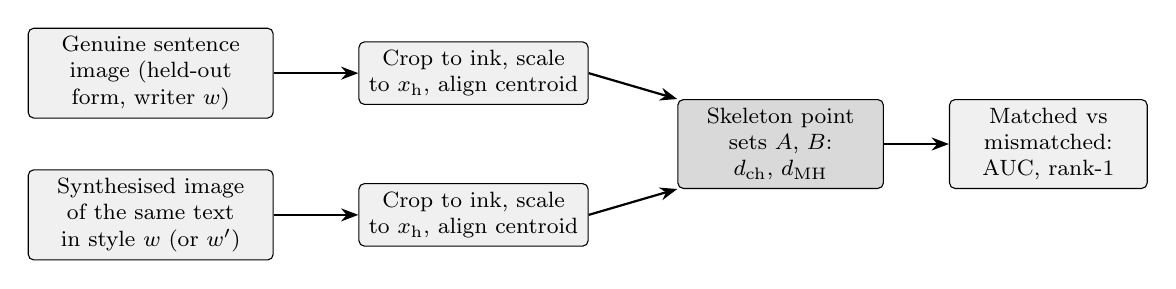
\begin{tikzpicture}[
  resbox/.style={draw,rounded corners=2pt,fill=gray!12,align=center,font=\footnotesize,minimum height=7mm,inner sep=3pt},
  resdark/.style={draw,rounded corners=2pt,fill=gray!30,align=center,font=\footnotesize,minimum height=7mm,inner sep=3pt},
  resarr/.style={-{Stealth[length=2.2mm]},thick}]
\node[resbox,text width=2.9cm] (real) at (0,0.9) {Genuine sentence image (held-out form, writer $w$)};
\node[resbox,text width=2.9cm] (syn) at (0,-0.9) {Synthesised image of the same text in style $w$ (or $w'$)};
\node[resbox,text width=2.7cm] (n1) at (4.1,0.9) {Crop to ink, scale to $x_{\mathrm{h}}$, align centroid};
\node[resbox,text width=2.7cm] (n2) at (4.1,-0.9) {Crop to ink, scale to $x_{\mathrm{h}}$, align centroid};
\node[resdark,text width=2.4cm] (d) at (8.0,0) {Skeleton point sets $A$, $B$: $d_{\mathrm{ch}}$, $d_{\mathrm{MH}}$};
\node[resbox,text width=2.3cm] (out) at (11.4,0) {Matched vs mismatched: AUC, rank-1};
\draw[resarr] (real)--(n1); \draw[resarr] (syn)--(n2);
\draw[resarr] (n1.east)--(d.north west); \draw[resarr] (n2.east)--(d.south west);
\draw[resarr] (d)--(out);
\end{tikzpicture}
\caption{Overlay test of qualification test 1: both images are normalised in the same way and matched writer pairs are compared with mismatched pairs.}
\label{fig:res-overlay}
\end{figure}

The skeleton point sets $A$ and $B$ that this procedure produces are compared with
\begin{equation}
\label{eq:res-chamfer}
d_{\mathrm{ch}}(A,B)=\frac{1}{2}\left[\frac{1}{\lvert A\rvert}\sum_{a\in A}\min_{b\in B}\lVert a-b\rVert+\frac{1}{\lvert B\rvert}\sum_{b\in B}\min_{a\in A}\lVert a-b\rVert\right],
\end{equation}
\begin{equation}
\label{eq:res-mhd}
d_{\mathrm{MH}}(A,B)=\max\left[\frac{1}{\lvert A\rvert}\sum_{a\in A}\min_{b\in B}\lVert a-b\rVert,\;\frac{1}{\lvert B\rvert}\sum_{b\in B}\min_{a\in A}\lVert a-b\rVert\right],
\end{equation}
\begin{equation}
\label{eq:res-auc}
\mathrm{AUC}=\Pr\left[d_{\mathrm{matched}}<d_{\mathrm{mismatched}}\right]+\tfrac{1}{2}\Pr\left[d_{\mathrm{matched}}=d_{\mathrm{mismatched}}\right],
\end{equation}
where $\lVert\cdot\rVert$ is the Euclidean norm and distances are in units of the x-height $x_{\mathrm{h}}$.
Equation~\ref{eq:res-chamfer} is the mean of the two directed mean nearest-neighbour distances, which symmetrises the one-directional chamfer matching distance of Barrow \emph{et al.}~\cite[pp.~659--660]{barrow1977}; Equation~\ref{eq:res-mhd} is their maximum, which is less sensitive to outliers than the classical Hausdorff distance~\cite{dubuisson1994}; and Equation~\ref{eq:res-auc} is the area under the receiver operating characteristic curve~\cite[p.~868]{fawcett2006}, 0.5 for a distance carrying no writer information and 1.0 for perfect separation.


The protocol sized this sub-test at 8 writers and 5 sentences, which gives 40 matched and $40\times9=360$ mismatched pairs; the run actually made used ten writers and three sentences each, which is the 30 matched and 300 mismatched pairs reported in Section~\ref{sec:res-qtp1}.
The features of Table~\ref{tab:res-features} are computed by one deterministic extractor with identical thresholds on every image, after cropping to the ink and binarising with the same rule.

\subsubsection{Positional error and its uncertainty budget}

The absolute error of a drawn cross and the uncertainty of its measurement, prescribed for qualification test~5 and never evaluated, are
\begin{equation}
\label{eq:res-r5}
e_i=\lVert\mathbf{p}_i-\mathbf{p}_i^{\mathrm{cmd}}\rVert,
\end{equation}
\begin{equation}
\label{eq:res-unc}
u=\sqrt{u_{\mathrm{scan}}^2+u_{\mathrm{ref}}^2+u_{\mathrm{id}}^2},
\end{equation}
where $\mathbf{p}_i$ is the measured and $\mathbf{p}_i^{\mathrm{cmd}}$ the commanded centre of cross $i$, referenced to the machine origin 5~mm inside the minimum end-stops.
In Equation~\ref{eq:res-unc}, $u_{\mathrm{scan}}$ is the scanner scale error obtained by scanning the verified ruler, $u_{\mathrm{ref}}$ the registration of the sheet against the machine origin and $u_{\mathrm{id}}$ the error of locating a cross centre, taken as half a pixel; the three standard uncertainties are combined in quadrature and the expanded uncertainty is $2u$, following the Guide to the Expression of Uncertainty in Measurement~\cite[Clause~5]{jcgm2008}.
Mean, maximum and 95th percentile of the error of Equation~\ref{eq:res-r5} were to be reported together with the uncertainty of Equation~\ref{eq:res-unc}, on the sheet reproduced blank as Table~\ref{tab:res-sheet}.
Because no mark was ever drawn, neither equation was evaluated.
}{}
\IfFileExists{4_Appendices/Appendix_res.tex}{%%
%%  Department of Electrical, Electronic and Computer Engineering.
%%  EPR400/2 Final Report - additional results.
%%
%%  Appendix 4 describes the appendix as the place where "while the main report
%%  should contain the main results, additional results may be given here".
%%  This file therefore holds only ADDITIONAL results and the blank measurement
%%  sheets of the tests that were not carried out.  No design equation, no
%%  component value and no headline measurement was moved here: those carry the
%%  design credit and stay in Section 3 and in Section 4.
%%

\subsection{Additional results and prepared measurement sheets}
\label{sec:app-res}

This appendix holds the supporting detail of the qualification tests of Section~\ref{sec:results}: the provenance of the data sets and model checkpoints behind every quoted figure, the two measurement sheets that were prepared for the sub-tests that were never carried out, the feature definitions prescribed for the style correlation, and the distance distributions behind the overlay test.
Every figure quoted against a requirement remains in Section~\ref{sec:results}; nothing here changes a result, and the blank sheets are reproduced so that the measurement that is missing is defined rather than merely named.

\subsubsection{Provenance of the data sets and checkpoints}
\label{sec:app-prov}

Section~\ref{sec:res-qtp} states two facts that qualify every figure in it, that the harness covers ten of the thirteen writers and that the live server serves an unmeasured text checkpoint.
This sub-subsection traces both to the stored files that establish them, so that the claims can be checked rather than taken on trust.

\emph{The ten-writer subset.}
The harness was run over the eight database writers 150, 151, 152, 153, 384, 551, 552 and 588 and the two personal writers Dylan and Yeukita.
The list is set by \texttt{PERSONAL\_AUTHORS} in \texttt{qtp\_scripts/qtp\_common.py}, which names only \texttt{yeukita} and \texttt{dylan}, and the stored results confirm it: in \texttt{qtp\_data/qtp1c\_results.json} the strings \texttt{abhinav}, \texttt{owen} and \texttt{thiya} occur zero times, while \texttt{dylan} occurs 72 times and \texttt{yeukita} 96 times.
The per-writer shape-judge accuracies that make those three the weakest of the set come from \texttt{stage4\_summary.json}.
The figures that do cover all thirteen writers come from the separate verification pipeline rather than the harness: the search-judge accuracy of qualification test~1, the per-writer end-to-end run of Figure~\ref{fig:res-e2e} and the 1358-line writer identification of qualification test~2.
The 669-crop recognition figure covers the five personal writers only, which is its own data set and not the ten-writer subset.
\mustdo{re-run the qualification-test harness with \texttt{PERSONAL\_AUTHORS} set to all five personal writers, so that the style-correlation, overlay and independent-judge figures cover the same thirteen writers as the rest of the chapter.}

\emph{The checkpoints.}
The character- and word-accuracy figures of qualification test~1 were measured with two text checkpoints recorded in \texttt{qtp\_data/qtp1c\_results.json}: \texttt{meta.production\_ckpt} is \texttt{paper\_cnn\_bilstm\_ctc\_joint\_best.pt}, the checkpoint inside the best-of-$N$ search, and \texttt{meta.heldout\_ckpt} is \texttt{paper\_cnn\_bilstm\_ctc\_hf\_best.pt}, the base model used as the judge outside the search.
The recognition figures of qualification test~2 were measured with the same joint checkpoint (\texttt{verify\_text\_accuracy.py}), and the writer-identification figures with \texttt{author\_classifier\_10new\_weights.pt} for ink and \texttt{author\_shape\_10new\_weights.pt} for shape.
The deployed recogniser is a different model: \texttt{Classify.py} prefers \texttt{paper\_cnn\_bilstm\_ctc\_scratch\_best.npz} over the converted checkpoints, and that file is present, so the from-scratch checkpoint is what the server loads.
Its two writer classifiers, by contrast, are the \texttt{.npz} conversions of the \texttt{.pt} files above and agree with them on 100\% of 1358 lines to within $8\times10^{-6}$ of logit, which is why the writer figures transfer to the deployed code and the text figures do not.
\mustdo{measure character and word accuracy of the deployed \texttt{paper\_cnn\_bilstm\_ctc\_scratch\_best.npz} checkpoint on the same 669 crops, or change the server to load the joint checkpoint that was measured.}
\mustdo{record the architecture width, layer count, parameter count, optimiser, learning-rate schedule, batch size and epoch count of each named checkpoint, so that every figure in Section~\ref{sec:results} is traceable to a trained model. No hyper-parameter table or parameter count is given for any of them at present.}

\subsubsection{Per-feature and per-judge breakdown of qualification test 1}

Section~\ref{sec:res-qtp1} quotes the style correlation as one pooled number and
the two-judge comparison as one difference; both are the summary of a per-item
breakdown, which is given here because it localises the defect rather than
merely sizing it.
Figure~\ref{fig:res-features} resolves the correlation into its nine features and
Figure~\ref{fig:res-judges} the character accuracy into the two checkpoints that
read the same sixty lines, while Figure~\ref{fig:res-matched} places the
synthesis beside genuine handwriting of the identical sentences.
Table~\ref{tab:res-perfeature} lists the per-feature coefficients that
Figure~\ref{fig:res-features} plots.

\begin{figure}[h]
\centering
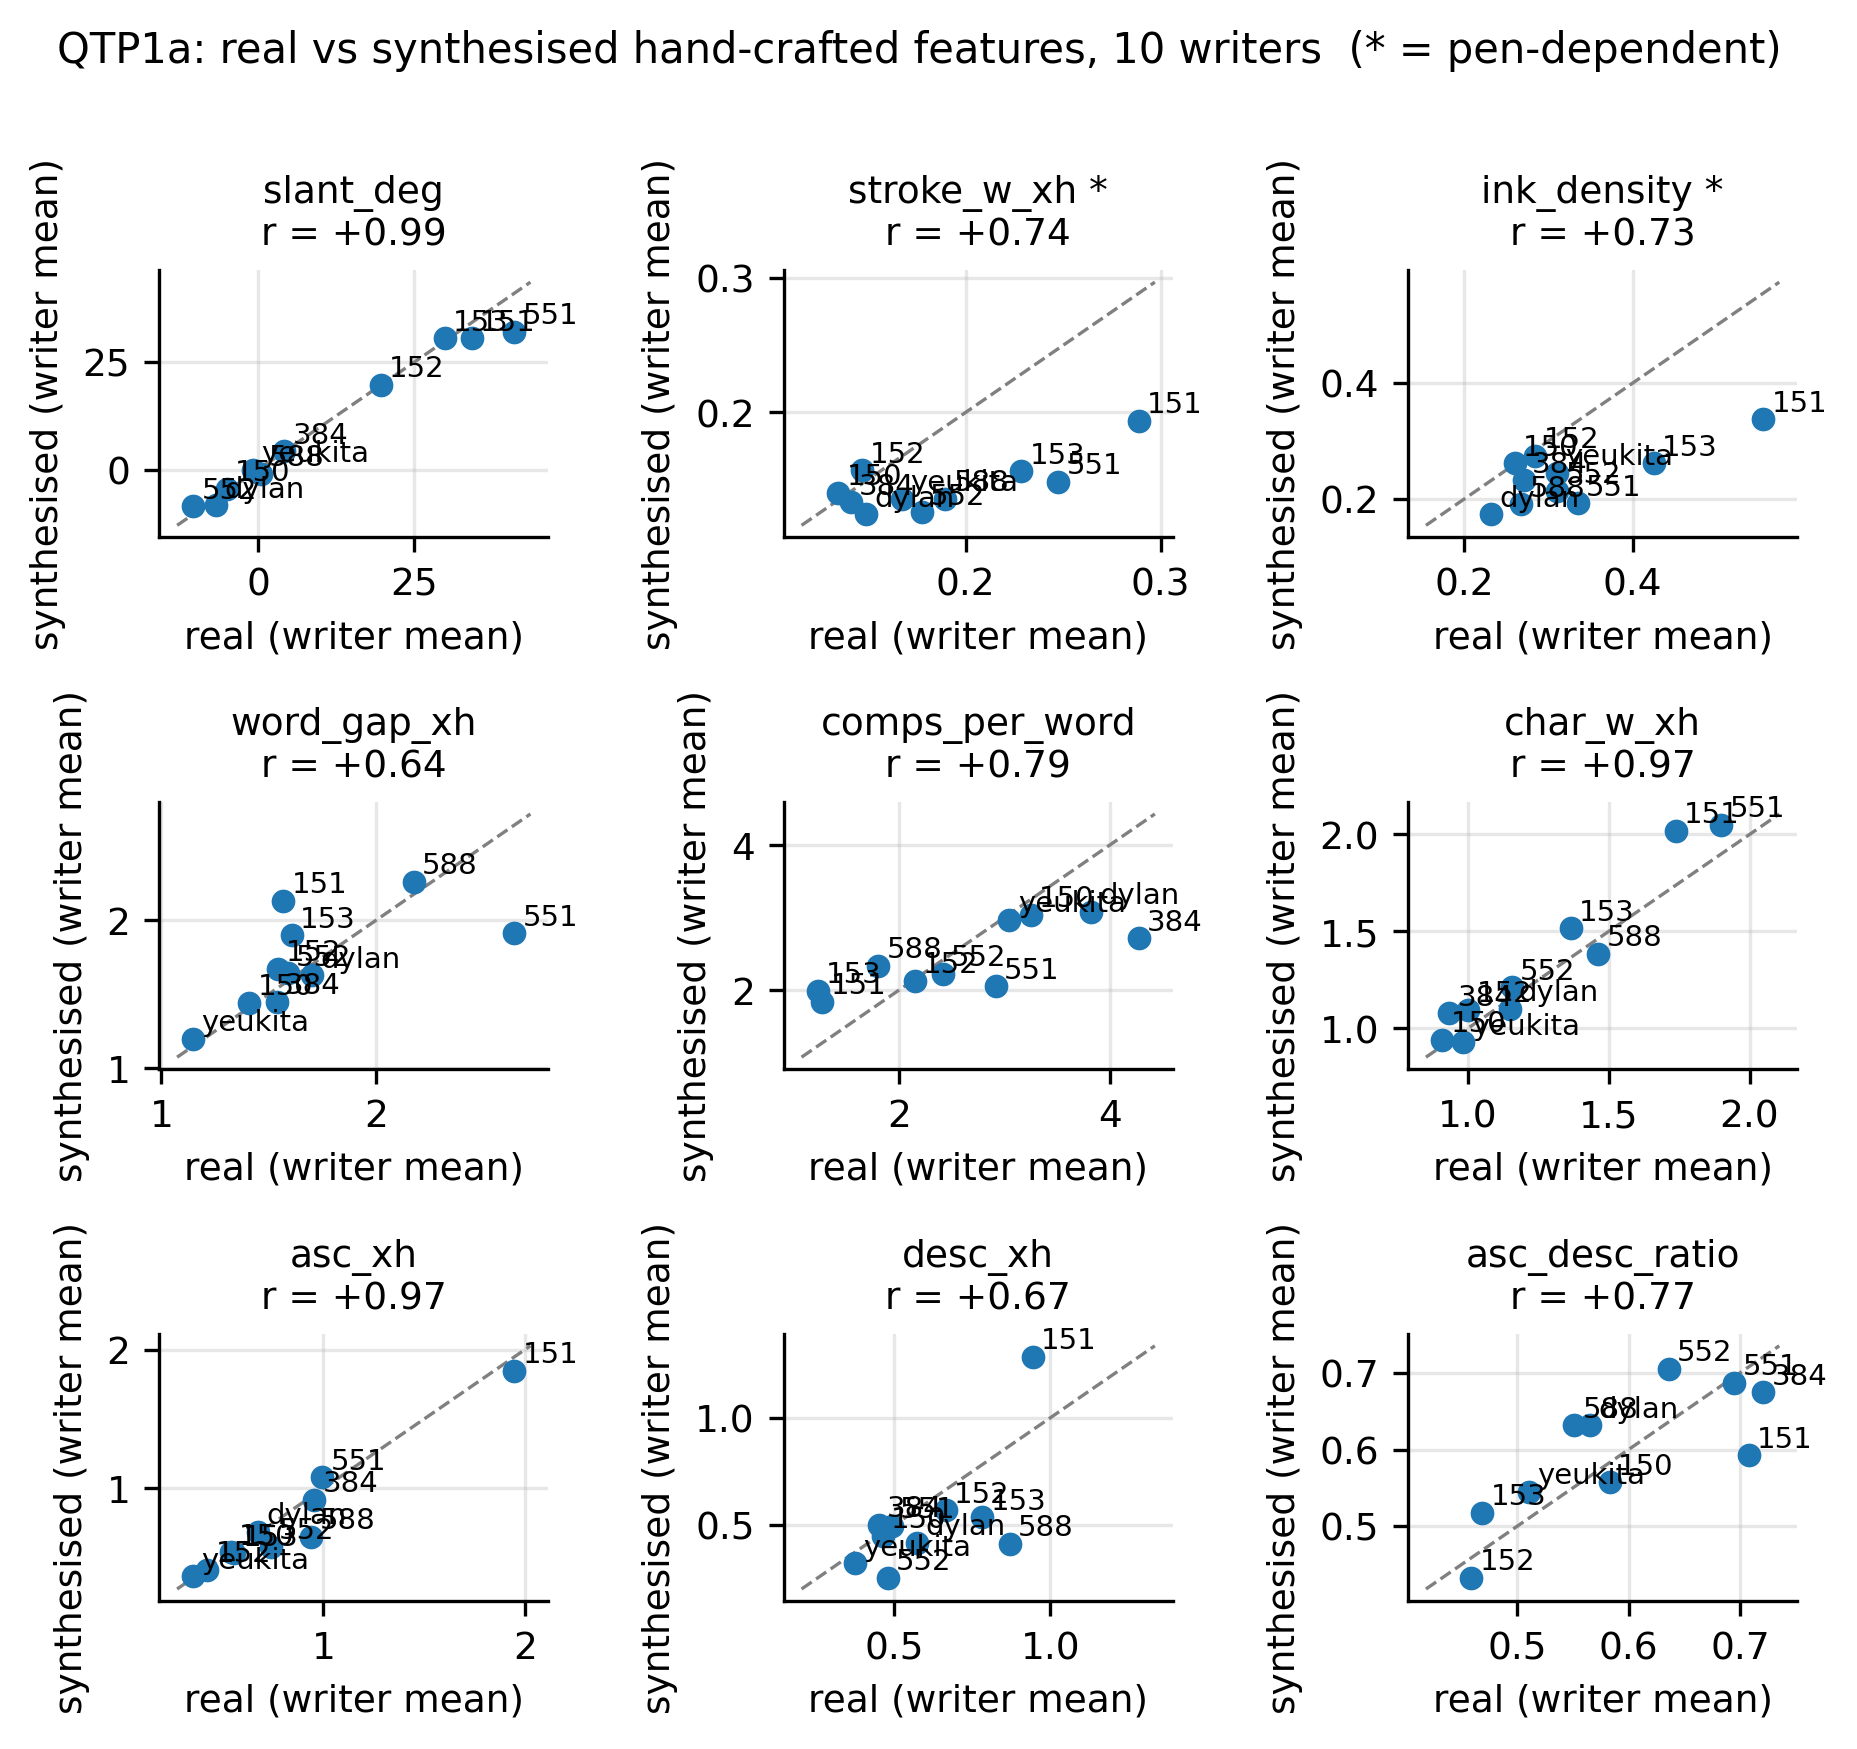
\includegraphics[width=0.99\linewidth]{Figures/qtp1_feature_scatter.png}
\caption{Style-correlation test on nine geometric features extracted by one deterministic routine from held-out real pages and from synthesised lines, for the ten writers. Each panel is one feature; the axes are the writer means. Slant, ascender and character width track the real hand closely, whereas descender and the ascender-to-descender ratio do not, which is the same defect that the word-accuracy gap identifies.}
\label{fig:res-features}
\end{figure}

\begin{figure}[h]
\centering
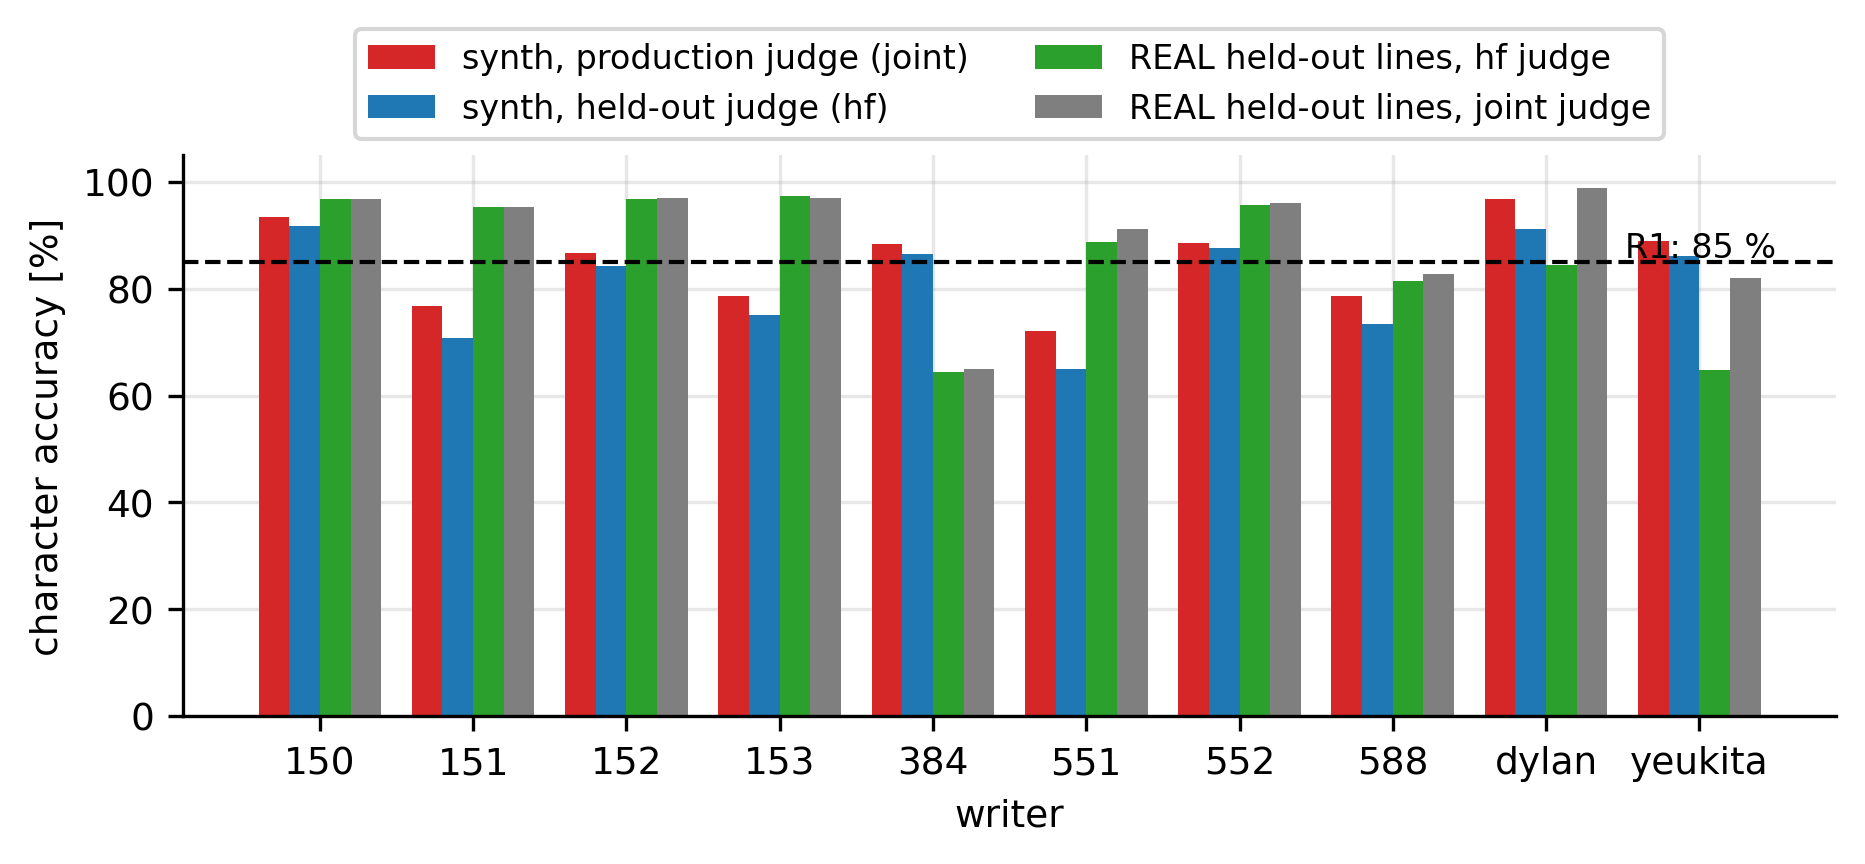
\includegraphics[width=0.85\linewidth]{Figures/qtp1_char_acc_judges.png}
\caption{Character accuracy of the synthesised text under the production recogniser and under a recogniser checkpoint that was not used to select the candidates. The independent judge scores the same output about three points lower, which quantifies how much of the apparent quality is a selection effect and simultaneously shows that the synthesis is genuinely legible rather than merely self-consistent.}
\label{fig:res-judges}
\end{figure}

\begin{figure}[h]
\centering
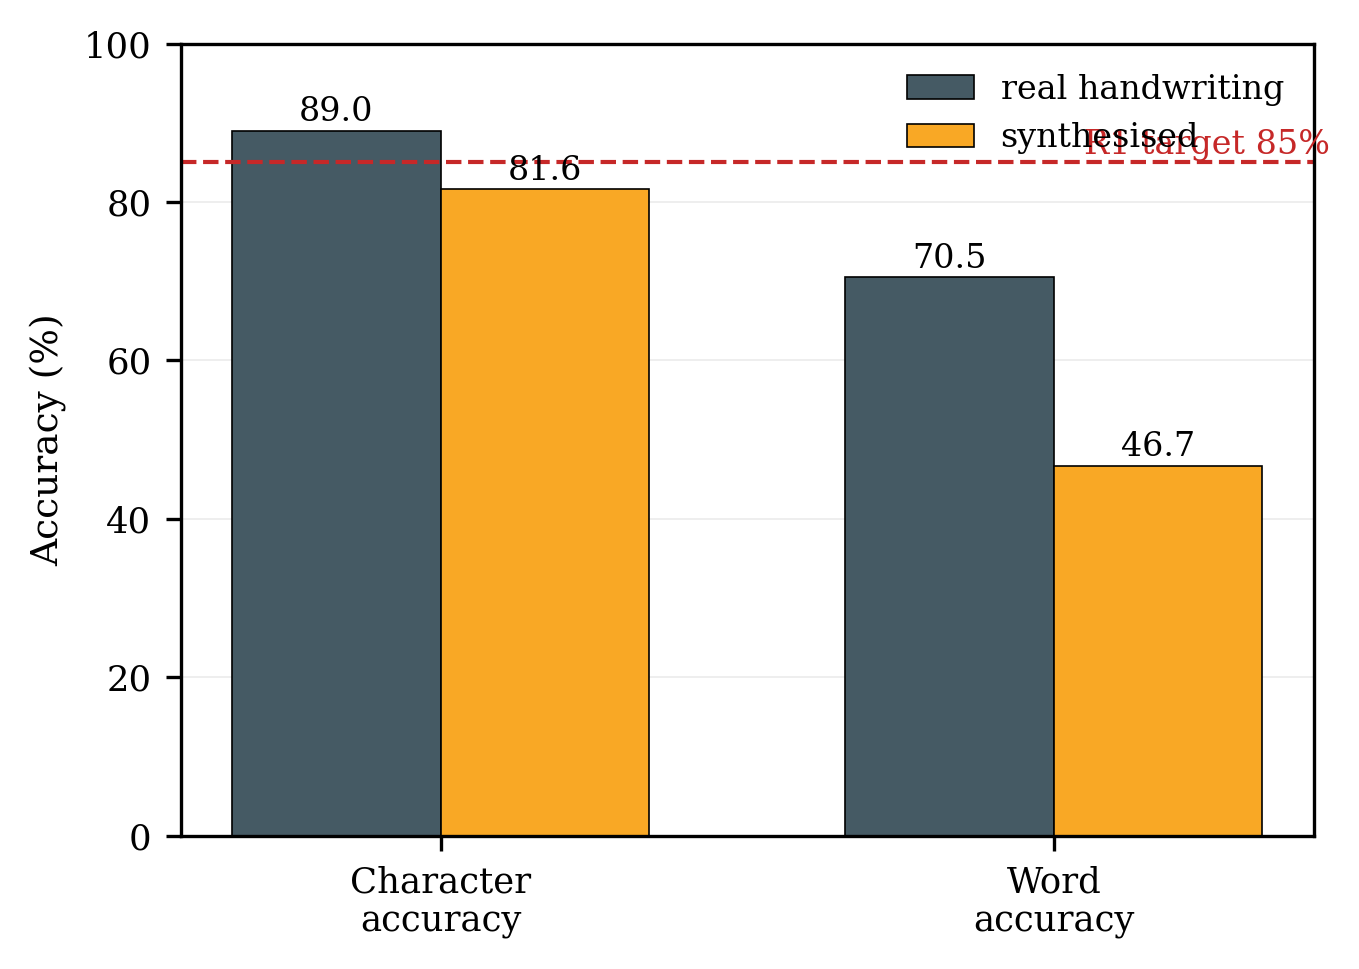
\includegraphics[width=0.85\linewidth]{Figures/res_matched_real_vs_synth.png}
\caption{Matching comparison on identical sentences: genuine handwriting of the sentence against the system's synthesis of that same sentence, both read by the same recogniser. Character accuracy is close to the target, but word accuracy divides by more than a factor of 1.5, which shows that the synthesis preserves letterforms better than it preserves word boundaries and spacing.}
\label{fig:res-matched}
\end{figure}

\begin{table}[h]
\centering
\fontsize{10}{12}\selectfont
\begin{tabularx}{\linewidth}{|>{\raggedright\arraybackslash}X|l|>{\raggedright\arraybackslash}X|l|}
\hline
\textbf{Feature} & \textbf{Pearson $r$} & \textbf{Feature} & \textbf{Pearson $r$} \\
\hline
Slant & 0.996 & Stroke width & 0.632 \\
\hline
Ascender extent & 0.974 & Word gap & 0.605 \\
\hline
Character width & 0.936 & Ascender-to-descender ratio & 0.509 \\
\hline
Components per word & 0.832 & Descender extent & 0.148 \\
\hline
Ink density & 0.680 & & \\
\hline
\end{tabularx}
\caption{Style correlation per feature across the ten harness writers, which
Figure~\ref{fig:res-features} plots and which the pooled coefficient of 0.714
reported in Table~\ref{tab:res-r1} summarises. The ordering is the result: slant
and the extent above the baseline are reproduced almost exactly, whereas the
extent below the baseline and the spacing between words are not.}
\label{tab:res-perfeature}
\end{table}


\subsubsection{Per-writer breakdowns}

The headline rates of qualification tests~1 and~2 are means over writers, and
the spread behind them is wider than the mean suggests, so the per-writer
breakdown is reproduced here in full.
Figure~\ref{fig:res-writerid} gives writer identification per writer over the
1358 real lines for both classifiers, Figure~\ref{fig:res-e2e} the end-to-end
result per writer through the G-code round trip, and
Table~\ref{tab:res-perwriter} the per-writer recognition accuracy behind the
98.61\% of qualification test~2.

\begin{figure}[h]
\centering
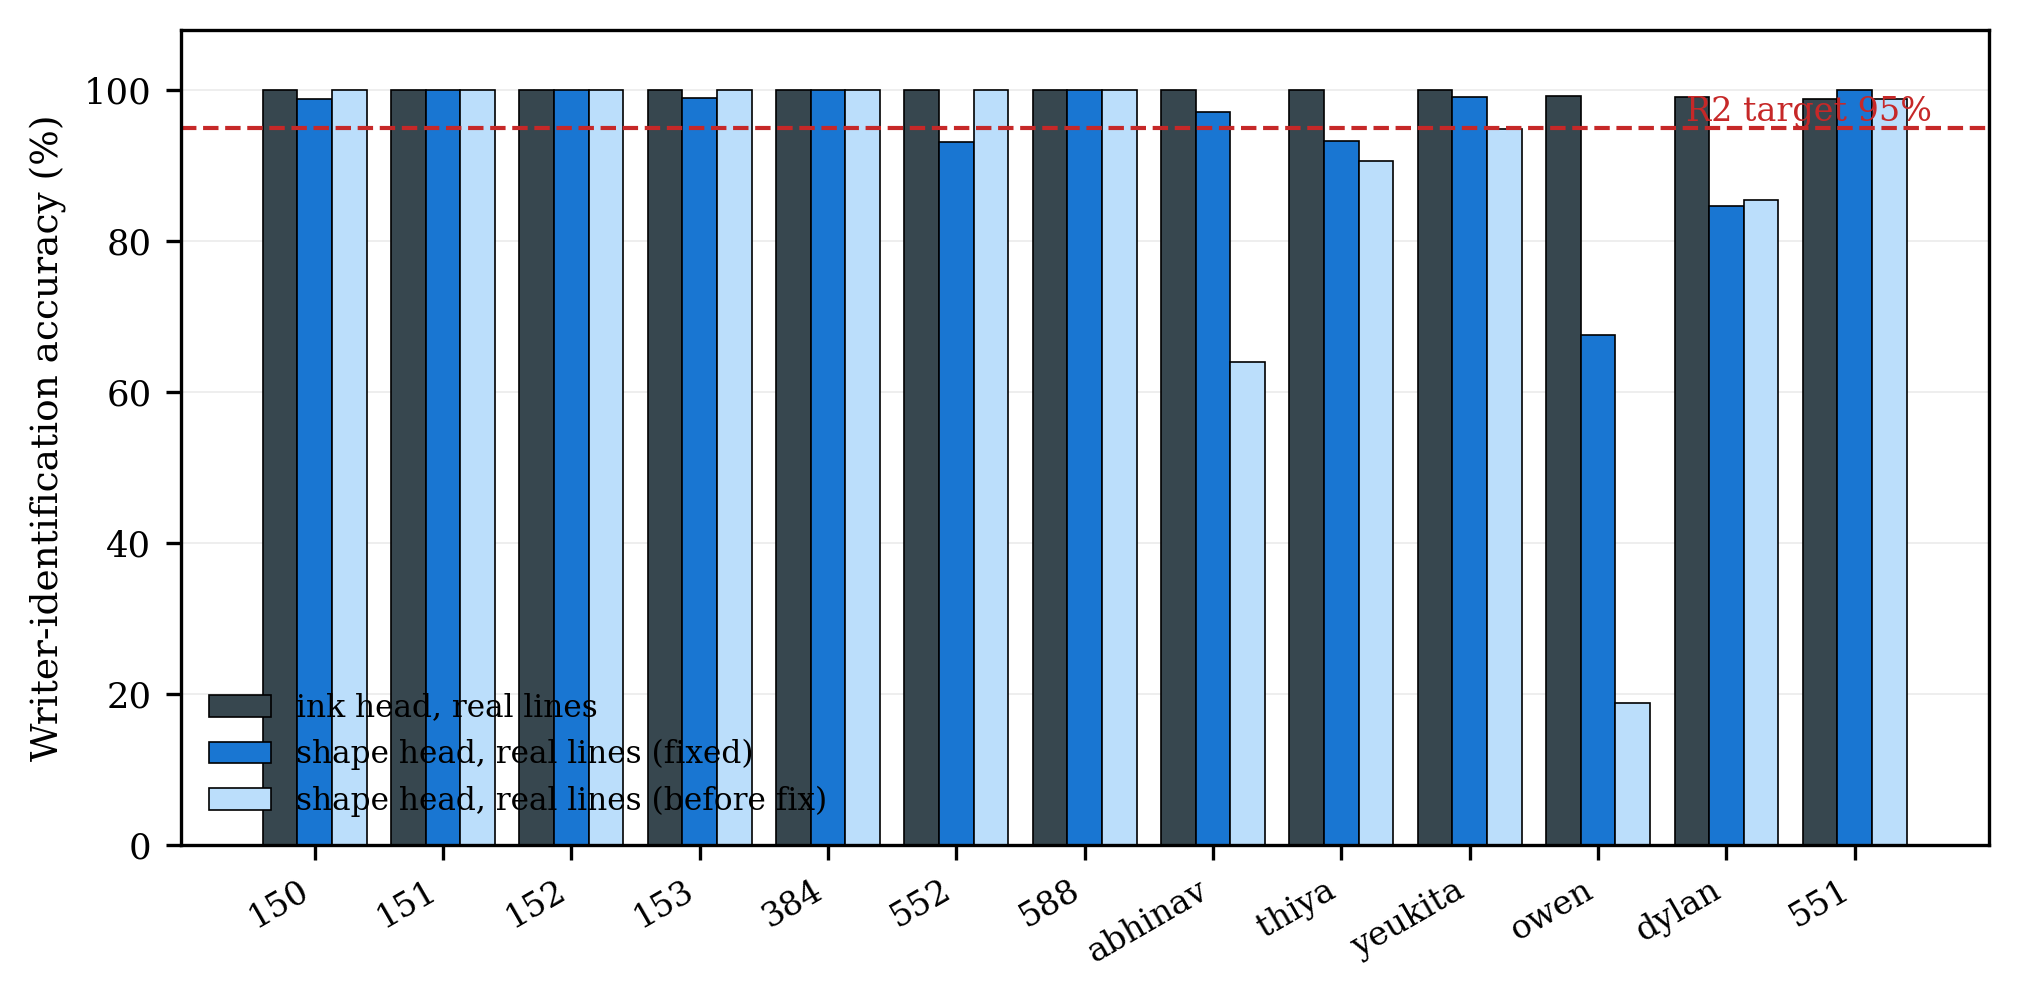
\includegraphics[width=0.85\linewidth]{Figures/res_writerid_per_author.png}
\caption{Writer-identification accuracy per writer over 1358 real lines, for the ink classifier and for the shape classifier before and after its training fault was corrected. The ink classifier is at or near 100\% for every writer. Correcting the shape classifier's training raised its overall accuracy from 83.4\% to 93.7\% and removed a systematic collapse in which 118 of Owen's 148 lines had been assigned to Yeukita. The dashed line is the 95\% target of R2.}
\label{fig:res-writerid}
\end{figure}

\begin{figure}[h]
\centering
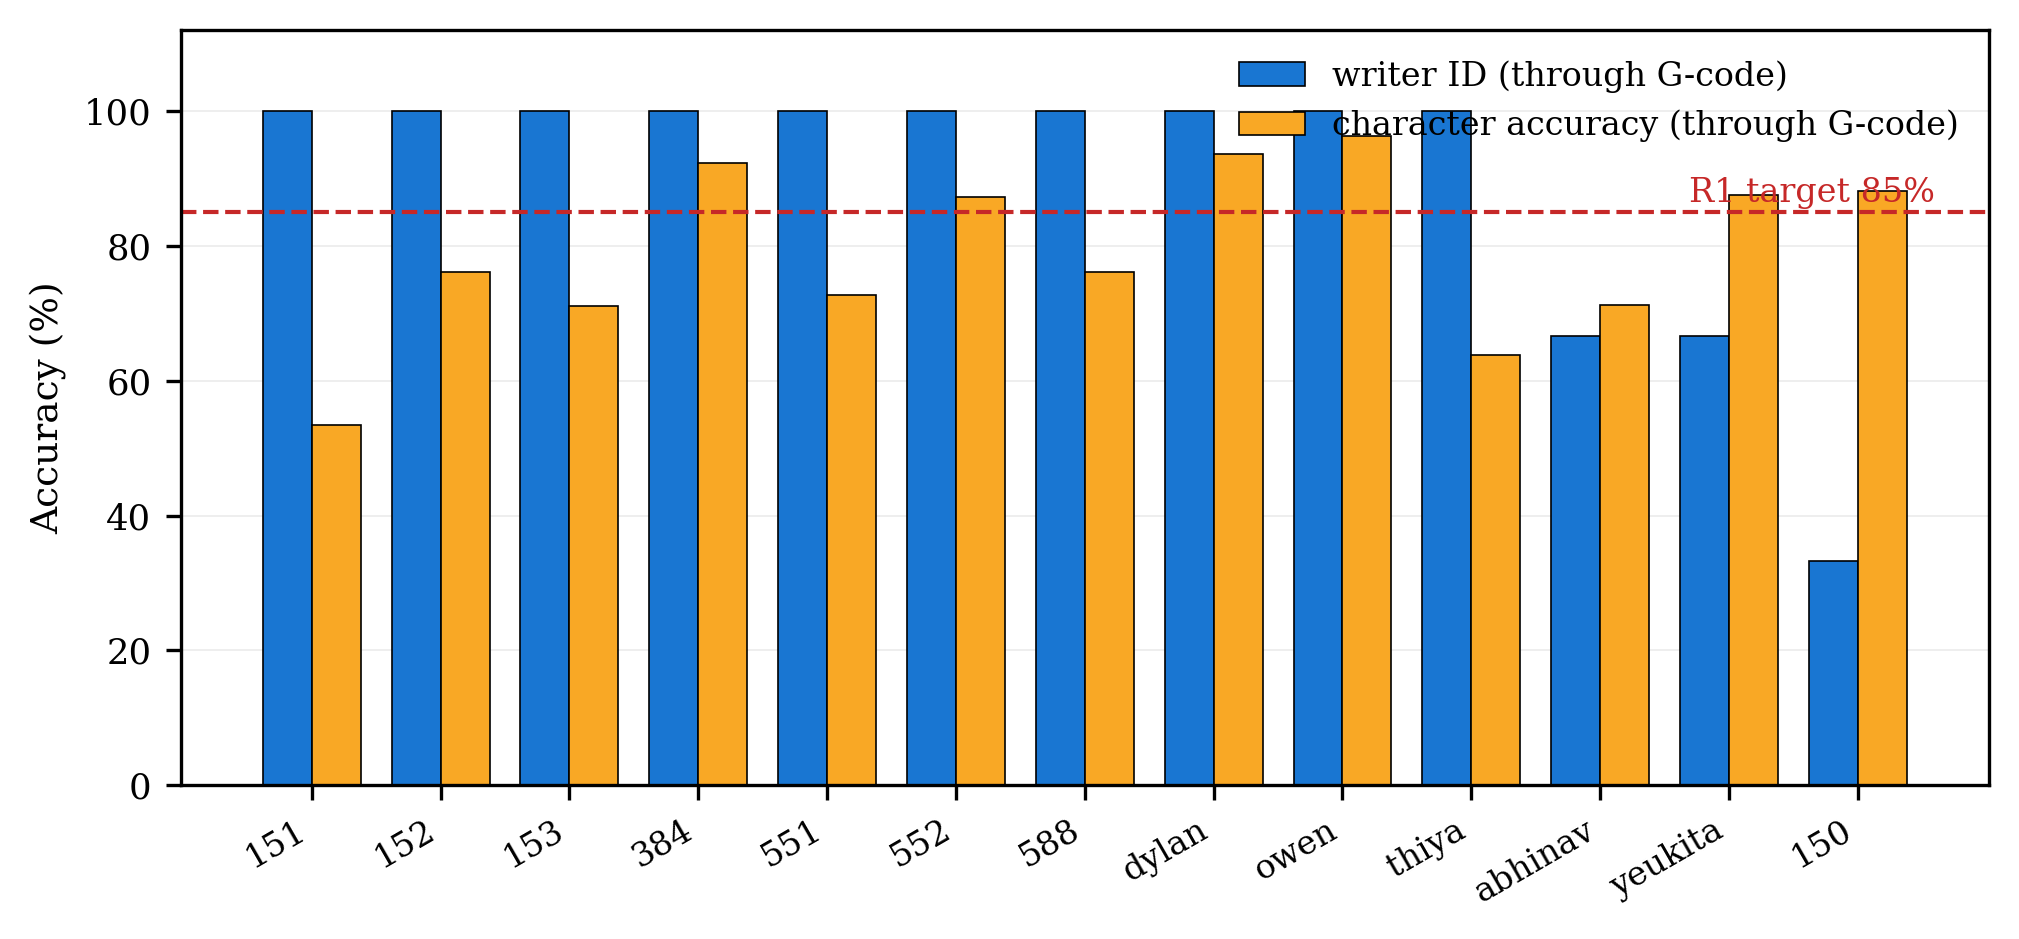
\includegraphics[width=0.85\linewidth]{Figures/res_e2e_per_author.png}
\caption{End-to-end result per writer over all thirteen writers: writer identification and character accuracy, both measured through the G-code round trip, for three novel sentences per writer at best-of-8 (\texttt{gcode\_v2\_summary.json}; shape judge \texttt{author\_shape\_10new\_weights}, text judge \texttt{paper\_cnn\_bilstm\_ctc\_joint\_best}). Ten of the thirteen writers are identified at 100\% by the shape judge; the remaining three are 150 at 33.3\% and Abhinav and Yeukita at 66.7\% each. The character-accuracy failures are concentrated in the two writers whose hands are the most joined, which is the known weak case of an exemplar synthesiser that cuts letters apart and reassembles them.}
\label{fig:res-e2e}
\end{figure}

\begin{table}[h]
\centering
\fontsize{10}{12}\selectfont
\begin{tabularx}{\linewidth}{|l|l|>{\raggedright\arraybackslash}X|}
\hline
\textbf{Writer} & \textbf{Character accuracy} & \textbf{Crops} \\
\hline
Owen & 99.15\% & 75 to 206 crops per writer; 669 in total \\
\hline
Dylan & 99.03\% & \\
\hline
Abhinav & 98.94\% & \\
\hline
Yeukita & 98.30\% & \\
\hline
Thiya & 96.46\% & \\
\hline
\end{tabularx}
\caption{Recognition accuracy per personal writer over the 669 real line crops of
qualification test 2, read by \texttt{paper\_cnn\_bilstm\_ctc\_joint\_best}. The
pooled figure is 98.61\%; Thiya, whose hand is the most joined of the five, is
the only writer more than two points below it.}
\label{tab:res-perwriter}
\end{table}


\subsubsection{Storage check of qualification test 6}

Qualification test~6 reduces to a count against a threshold, and
Figure~\ref{fig:res-storage} is the observation behind that count.

\begin{figure}[h]
\centering
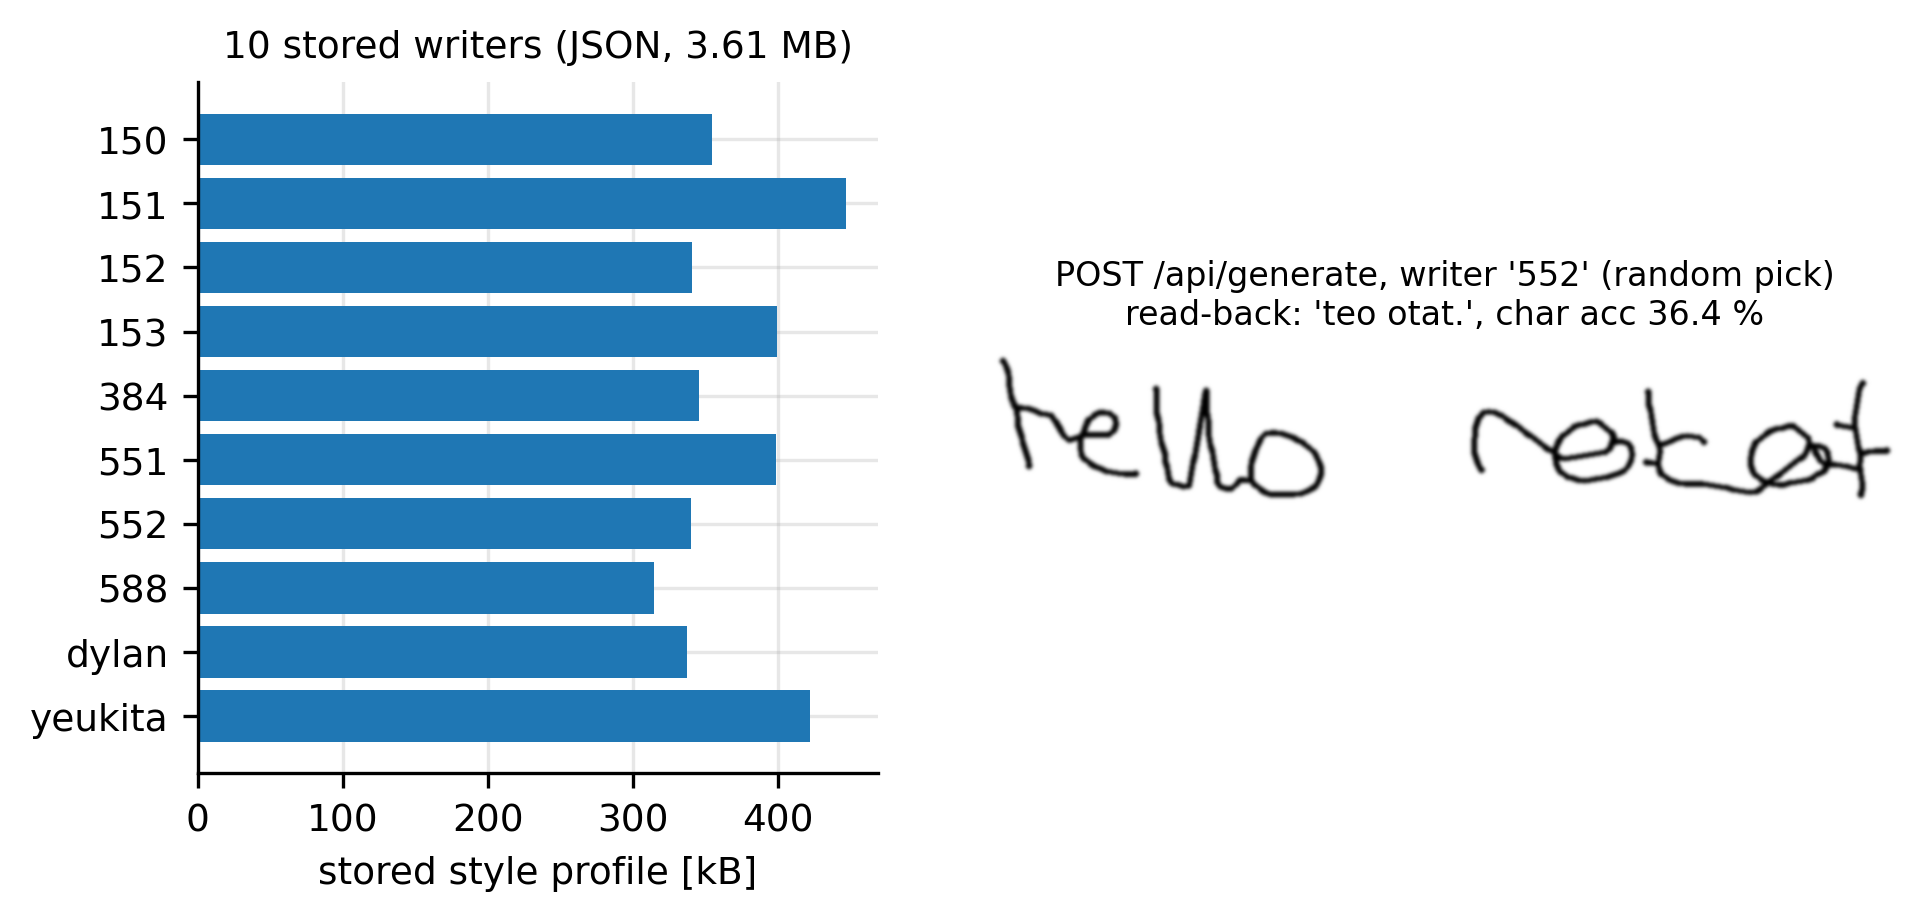
\includegraphics[width=0.85\linewidth]{Figures/qtp6_storage.png}
\caption{Storage of the writing styles. Each writer is held as a style profile and the server lists all thirteen through its author-list endpoint, against the ten required by R6.}
\label{fig:res-storage}
\end{figure}

\subsubsection{Prepared sheets for the sub-tests not carried out}

Two sub-tests were specified in full and never executed, sub-test~(d) of qualification test~1 (the blind human panel) and qualification test~5 (absolute positional error).
Table~\ref{tab:res-panel} is the worksheet printed for the panel and Table~\ref{tab:res-sheet} the data sheet printed for the positional measurements.
Both are shown exactly as printed, that is to say blank, because no rater was convened and no cross was ever drawn.

\begin{table}[h]
\centering
\fontsize{10}{12}\selectfont
\begin{tabularx}{\linewidth}{|l|X|l|l|}
\hline
\textbf{Line no.} & \textbf{Transcription written by the rater (without hint of the content)} & \textbf{Illegible characters (positions)} & \textbf{Confidence (1--5)} \\
\hline
1 & & & \\
\hline
2 & & & \\
\hline
$\vdots$ & & & \\
\hline
40 & & & \\
\hline
\end{tabularx}
\caption{Worksheet prepared for the blind human panel of qualification test 1: 30 synthesised lines and 10 genuine control lines in random order. The panel was never convened, so no worksheet was completed and the table is shown blank as it was printed.}
\label{tab:res-panel}
\end{table}

\begin{table}[h]
\centering
\fontsize{10}{12}\selectfont
\begin{tabularx}{\linewidth}{|l|l|l|l|l|l|X|}
\hline
\textbf{Repeat} & \textbf{Cross} & \textbf{$x^{\mathrm{cmd}}$ (mm)} & \textbf{$y^{\mathrm{cmd}}$ (mm)} & \textbf{$x$ meas. (mm)} & \textbf{$y$ meas. (mm)} & \textbf{$e_i$ (mm)} \\
\hline
1 & 1 & & & & & \\
\hline
1 & 2 & & & & & \\
\hline
$\vdots$ & & & & & & \\
\hline
\end{tabularx}
\caption{Data sheet prepared for the absolute positional error of qualification test 5; one row per cross and repetition, together with the scanner scale check and the registration check. No row was ever completed, because the test was not carried out.}
\label{tab:res-sheet}
\end{table}

\subsubsection{Features prescribed for the style correlation}

The style-correlation sub-test of qualification test~1 compares geometric features extracted by one deterministic routine from held-out real pages and from synthesised lines.
Table~\ref{tab:res-features} defines the features as they were prescribed in the protocol; the extractor that produced the measured correlation implements this set extended to the nine features reported in Table~\ref{tab:res-r1}.
The definitions are given here rather than in Section~\ref{sec:results} because they fix the measurement rather than report a result.

\begin{table}[h]
\centering
\fontsize{10}{12}\selectfont
\begin{tabularx}{\linewidth}{|>{\raggedright\arraybackslash}p{3.3cm}|X|}
\hline
\textbf{Feature} & \textbf{Definition} \\
\hline
Slant & Shear angle (degrees) that maximises the variance of the column ink projection of the line. \\
\hline
Stroke width & Median stroke width from the distance transform at the skeleton, divided by $x_{\mathrm{h}}$. \\
\hline
Ink density & Fraction of ink pixels inside the core band between the baseline and the x-height line. \\
\hline
Word gap & Median horizontal gap between words (gaps larger than $0.5\,x_{\mathrm{h}}$) divided by $x_{\mathrm{h}}$. \\
\hline
Connectedness & Number of connected ink components divided by the number of characters of the text. \\
\hline
Character width & Line width divided by the number of characters, divided by $x_{\mathrm{h}}$. \\
\hline
Ascender/descender ratio & (Height of the ascender zone plus depth of the descender zone) divided by $x_{\mathrm{h}}$. \\
\hline
\end{tabularx}
\caption{Hand-crafted style features prescribed for the correlation and retrieval of qualification test 1. The extractor that produced the measured correlation implements this set extended to the nine features listed in Table~\ref{tab:res-r1}.}
\label{tab:res-features}
\end{table}

\subsubsection{Distance distributions behind the overlay test}

The overlay test of qualification test~1 reduces to two numbers in Table~\ref{tab:res-r1}, the ratio of matched to mismatched distance and the area under the curve.
Figure~\ref{fig:res-dist} gives the distributions those two numbers summarise, which show how far the two populations actually overlap.

\begin{figure}[h]
\centering
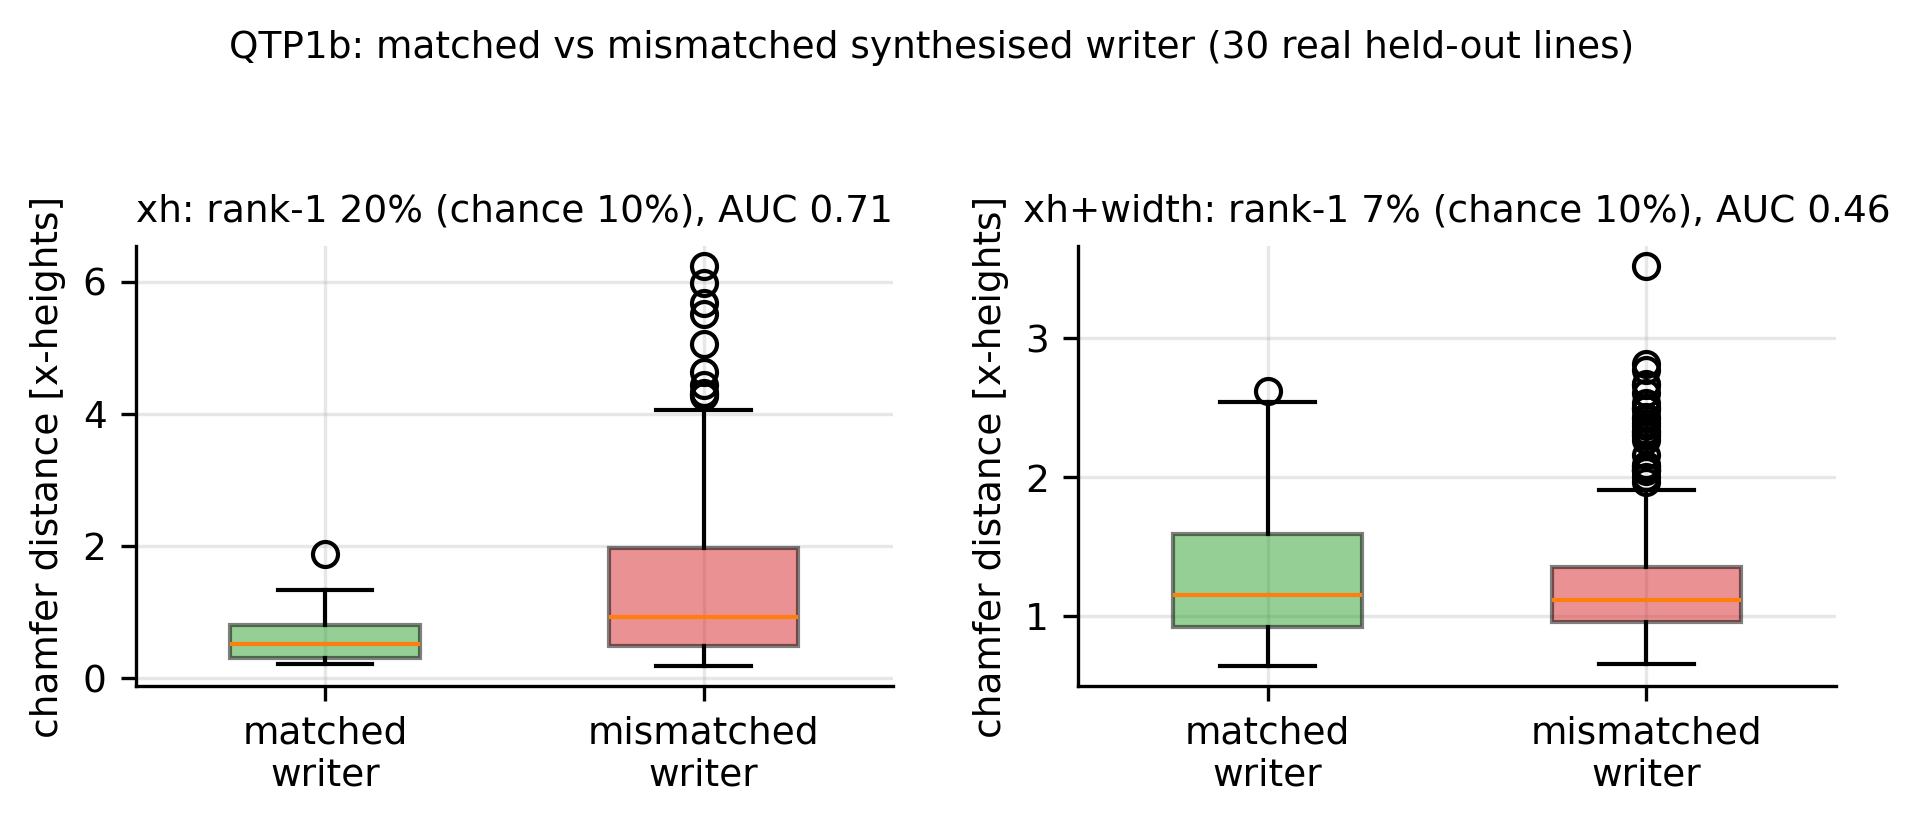
\includegraphics[width=0.93\linewidth]{Figures/qtp1_matched_vs_mismatched.png}
\caption{Distributions of the matched and mismatched overlay distances. The two distributions overlap but their means are separated by a factor of about 2.2 on the chamfer measure, giving an AUC of 0.71: the synthesis carries real writer information, but it is far from indistinguishable from the hand it imitates.}
\label{fig:res-dist}
\end{figure}
}{}
\IfFileExists{4_Appendices/Appendix_app.tex}{\input{4_Appendices/Appendix_app}}{}
\IfFileExists{4_Appendices/Appendix_seg.tex}{%%
%%  Department of Electrical, Electronic and Computer Engineering.
%%  EPR400/2 Final Report - supporting detail of the segmentation block.
%%
%%  Section 3.4 gives the six stages, the equations that define each one and
%%  the measured limitations.  This file holds the detail: the full constant
%%  table, the eight artefact-discard predicates, the six pixel-ownership
%%  correction rules and pseudocode of the four routines that carry the
%%  arithmetic.  Every threshold here is a multiple of the measured line pitch,
%%  which is the point of the table.  No code is reproduced; the routines are
%%  given as pseudocode.
%%

\subsection{Supporting detail of the page conditioning and segmentation block}
\label{sec:app-seg}

Section~\ref{sec:segmentation} describes the six stages of the segmentation block and the equations that define each of them.
This appendix carries the three tables of constants and rules that the stage descriptions refer to, together with pseudocode of the four routines in which the arithmetic actually happens.
It is here rather than in Section~\ref{sec:segmentation} because it enumerates thresholds rather than explaining the design: the design decision is that almost every threshold is a multiple of the measured line pitch $P$, and these tables are the evidence that it is.

\subsubsection{Constants of the minor operations}

Table~\ref{tab:seg-const} collects every constant of the minor operations of all six stages with the reason for each, so that the stage descriptions of Section~\ref{sec:segmentation} can keep to the operations themselves.
Only four entries are not expressed in units of the pitch, and those four are identified in the caption.

\begin{table}[!htbp]
\centering
\fontsize{8}{9.4}\selectfont
\setlength{\tabcolsep}{3.5pt}
\renewcommand{\arraystretch}{1.05}
\begin{tabularx}{\linewidth}{|c|p{5.1cm}|X|}
\hline
\textbf{St.} & \textbf{Quantity and value} & \textbf{Reason} \\
\hline
2 & Otsu histogram over $[0,1.2]$, 256 bins & paper sits at $\rho\approx1$ and nothing above 1.2 carries ink information, so a highlight cannot drag the cut \\
\hline
2 & solid-area veto $\mathrm{BoxMean}_4(\mathrm{ink})>0.999$, cleared over $7\times7$ & no pen stroke fills a $9\times9$ window; the fringe goes with the blob, and 0.999 absorbs integral-image rounding \\
\hline
3 & 17 angles, $-4.0^\circ$ to $+4.0^\circ$ in $0.5^\circ$ & one sweep, no refinement, over a sixteenth of the photograph's area \\
\hline
3 & rotation fill 0 for the candidate masks, 255 for the page & outside the sheet must add no ink to the profile; corners brought in must be white paper \\
\hline
4 & paper region: block-average by $s=4$, blur $\max(1,\lfloor0.15P/s\rfloor)$, dark below $0.45\times$ median & a ratio and not a grey level, so it survives a change of exposure \\
\hline
4 & whole frame accepted as paper below $0.2\,\%$ dark cells; sheet eroded $\lfloor0.4P\rfloor$ per axis & correct for a photograph filled by the sheet; the erosion keeps the sheet's darkened rim out of the ink mask \\
\hline
4 & piece closing $\max(1,\lfloor0.1P\rfloor)$ & bridges the pen lifts inside a word, so a word is one piece \\
\hline
5 & centre separation $0.6P$ & more than half a pitch, so two genuine lines can never be merged \\
\hline
6 & seam closing $\max(2,\lfloor0.07P\rfloor)$ & fills only the gap beside a letter stem; a dilation would make a blob the cut would trace \\
\hline
6 & outer boundaries $\lfloor0.75P\rfloor$ beyond the first and last centre & covers the first line's ascenders and the last line's descenders \\
\hline
6 & band emitted above $\max(60,\,0.12\,\mathrm{median}_n N_n)$ owned pixels and $\max(6,\,0.2P)$ rows & keeps a short line carrying an eighth of the typical ink; the absolute 60 catches a tiny-median page \\
\hline
6 & vertical gap trimmed only if it removes more than $0.8P$ & spares the ordinary gap between a line's body and its own ascenders \\
\hline
6 & crop padding $\lfloor0.15P\rfloor$ per side, halo $\lfloor0.20P\rfloor$ per axis, local recovery radius $\max(3,\min(20,\mathrm{round}(h_{\mathrm{crop}}/8)))$ & the halo anchors recovery to ink the line already owns; the local radius judges a pale line against its own contrast \\
\hline
6 & stretch of Equation~\ref{eq:seg-stretch}: $b$ the 40th percentile under the mask, $w$ the 75th of the crop & the 40th percentile is the typical ink darkness, so one dark speck cannot flatten the line \\
\hline
\end{tabularx}
\caption{Constants of the minor operations of each stage of the segmentation block, with the reason for each. Every entry in units of the measured pitch $P$ scales with the page; the four that do not are the Otsu range, the $0.2\,\%$ and $0.45$ paper-region tests and the floor of 60 ink pixels. The constants of the core operations appear in the equations of Section~\ref{sec:segmentation} itself.}
\label{tab:seg-const}
\end{table}

\subsubsection{The eight artefact-discard predicates}

Stage~4 judges each closed piece of ink as a whole and discards it if any one of eight predicates holds.
Table~\ref{tab:seg-artifact} states them with the nuisance each is meant to catch, for a piece of area $A$, height $h$ and width $w$, with $e=\max(3,\lfloor0.5P\rfloor)$ counting as touching the frame, $x_L$ the fifth percentile of the left edges of the letter-like pieces ($A\ge0.065P^2$, $h\le2.2P$) and faintness defined as $\bar\rho_c>0.85\,t^*$, relative to the page's own threshold so that one constant serves pencil and fibre tip.

\begin{table}[h]
\centering
\fontsize{8.5}{10.2}\selectfont
\setlength{\tabcolsep}{4pt}
\begin{tabularx}{\linewidth}{|p{3.3cm}|X|}
\hline
\textbf{Discard condition} & \textbf{What it is meant to catch} \\
\hline
$x_{\min}\le e$ & A piece touching the left frame edge: the facing page, or the desk. \\
\hline
$x_{\max}\ge W-1-e$, $w\le0.5P$ & A narrow sliver at the right edge; a real line there is wider. \\
\hline
$y_{\min}\le e$ or $y_{\max}\ge H-1-e$, $h\le0.5P$, $w\le0.5P$ & A small fleck at the top or bottom frame edge. \\
\hline
$h>2.2P$, $w\le0.5P$ & A tall thin streak over two line spacings: a binder edge or a fold. \\
\hline
$w\le0.12P$, $h\ge1.2P$ & A bar thinner and taller than any letter. \\
\hline
$\mathrm{faint}$, $w\le0.2P$, $h\ge0.6P$ & A printed margin rule or a crease. \\
\hline
$(y_{\min}\le e$ or $y_{\max}\ge H-1-e)$, $h\le1.2P$, $A/(hw)<0.15$, $\mathrm{faint}$, $w>P$ & An edge shadow or fold: wide, faint, at an edge, too sparse inside its own box to be writing. \\
\hline
$x_{\max}<x_L-1.2P$ & A hole punch, a staple shadow or a page number in the gutter. \\
\hline
\end{tabularx}
\caption{The eight discard predicates applied to each closed piece of ink in stage~4; the background label is exempt from all of them. The first row is the most aggressive rule in the module: any piece whose leftmost ink lies within $e$ of the left frame edge is discarded whatever its size or darkness, which removes the facing page of an open book but also costs the first letters of a page photographed with no left margin.}
\label{tab:seg-artifact}
\end{table}

\subsubsection{The six pixel-ownership correction rules}

By default an ink pixel belongs to the band it lies in, and stage~6 then applies six correction rules on top of that default, each of which may move a piece to an adjacent band or drop it but never further.
Table~\ref{tab:seg-own} states them.
They rest on each band's share of a piece's ink, with $0.15$ counting as a genuine presence, and on the \emph{major} band, defined as the topmost band reaching the piece, since a piece spanning two lines is the upper one's descender.

\begin{table}[h]
\centering
\fontsize{8.5}{10.2}\selectfont
\setlength{\tabcolsep}{4pt}
\begin{tabularx}{\linewidth}{|p{0.7cm}|p{3.6cm}|X|}
\hline
\textbf{Rule} & \textbf{Applies to} & \textbf{Action, and the reason for it} \\
\hline
1 & A remnant in a band adjacent to the major band: under $0.12P^2$ there, under $0.35$ of the piece's ink, no wider than $0.55P$ & Returned to the major band. The width test separates a cut-off tail, which is narrow, from a genuine short word, which is wide. \\
\hline
2 & A piece under $0.06P^2$; a \emph{speck} is under $0.01P^2$ & Dropped if no \emph{big} piece ($\ge0.05P^2$) of its own line lies within $6P$ horizontally, else moved one band towards the body it belongs to, asymmetrically ($0.5P$ below, $0.7P$ above), because a mark below a line is usually its own comma or descender while one well above it is more often an accent of the line above. A speck out of band drops rather than moves. \\
\hline
3 & A piece of $0.06P^2$ to $0.15P^2$ & Given to whichever of the three nearest bands has its body closest in $y$. \\
\hline
4 & A \emph{dot}: area under $0.1P^2$, extent at most $0.45P$, aspect ratio under 2.2 so that a short dash does not qualify & Followed downwards up to $\lfloor0.4P\rfloor$ rows to the first \emph{stem} ($\ge0.03P^2$) and moved to that stem's band only if that band's body also lies $0.25P$ to $0.7P$ below it, where an $i$ dot sits relative to its own x-height band. Together the two conditions are much stronger than either alone, since the scan can meet the wrong stem on a crowded page and the band test can accept a mark belonging to no stem. \\
\hline
5 & The same search on the raw, unclosed labelling, for pieces of at least $0.015P^2$ & Catches a dot the stage-4 closing has welded to a descender of the line above. A ring-footed stroke the same welding makes --- a blob of width $0.2P$ to $0.45P$, aspect ratio $0.6$ to $1.6$ --- also follows the stem below, but only if it encloses a hole, since a dot ring does and a hook does not. Neither rule reassigns a whole word ($\ge0.2P^2$). \\
\hline
6 & A fragment of at least $0.006P^2$ with no ink within $0.28P$ of its own band's centre & Offered to the line whose ink it touches, or failing that to the nearer neighbouring centre if the fragment sits within $0.2P$ of it. Fragments placed by rule~5 are locked, since a dot deliberately lifted into a band would otherwise be pushed straight back. \\
\hline
\end{tabularx}
\caption{The pixel-ownership correction rules of stage~6. The size ladder they share runs $0.006P^2$, $0.01P^2$, $0.015P^2$, $0.03P^2$, $0.05P^2$, $0.065P^2$, $0.1P^2$, $0.12P^2$ and $0.2P^2$, every entry a multiple of the measured pitch squared, so no rule is tied to a pixel count.}
\label{tab:seg-own}
\end{table}

\subsubsection{Pseudocode of the four routines that carry the arithmetic}

Four routines account for almost all of the block's arithmetic, and each is given here as pseudocode.
The first shows why the three array primitives of Section~\ref{sec:segmentation} cost the same whatever the window radius: each is two cumulative sums and a slice difference, so none contains a loop over pixels.

\begin{figure}[h]
\centering
\fontsize{8.5}{10.2}\selectfont
\begin{verbatim}
  BoxMean( image, radius r ):            # mean over a (2r+1)x(2r+1) window
      pad the image by r, replicating the edge
      integral <- cumulative sum down, then cumulative sum across
      return ( four corner look-ups into integral ) / (2r+1)^2

  AnyWithinRadius( mask, radius r, axis ):          # one-axis dilation
      c <- cumulative sum of the mask along the axis
      return ( c[ i+2r+1 ] - c[ i ] ) > 0     for every position i

  LongRunMask( mask, length n, axis ):   # pixels on a run of n or more
      c   <- cumulative sum of the mask along the axis
      hit <- ( c[ i+n ] - c[ i ] ) = n        # a run of n starts at i
      ch  <- cumulative sum of hit
      return ( ch[ high ] - ch[ low ] ) > 0   # some such run covers i
\end{verbatim}
\caption{The three array primitives of the segmentation block as pseudocode. \texttt{BoxMean} is Equation~\ref{eq:seg-sat}, \texttt{AnyWithinRadius} is Equation~\ref{eq:seg-dilate} and \texttt{LongRunMask} is Equation~\ref{eq:seg-runmask}. Because each is built on a cumulative sum, a window of any size costs four look-ups, which is what makes the 40-pixel illumination blur of stage~2 affordable.}
\label{fig:seg-primspseudo}
\end{figure}

Stage~2 is four array statements and holds no tunable grey level, which is the result of dividing the illumination out before thresholding rather than after.

\begin{figure}[h]
\centering
\fontsize{8.5}{10.2}\selectfont
\begin{verbatim}
  OtsuThreshold( values ):
      histogram <- 256 bins of the values clipped to [0, 1.2]
      w, m      <- cumulative class weight and cumulative class mean
      variance  <- ( total mean . w  -  m )^2 / ( w . (1 - w) )
      return the bin centre maximising variance

  InkMask( grey ):
      r     <- max( 8, min( 40, round( image height / 41 ) ) )
      ratio <- grey / max( BoxMean( grey, r ), 1 )      # divide, not subtract
      mask  <- ratio < OtsuThreshold( ratio )
      solid <- BoxMean( mask, 4 ) > 0.999    # a 9x9 window wholly ink
      return mask AND NOT ( dilate solid by 3 ),  ratio
\end{verbatim}
\caption{Lighting normalisation and the ink mask as pseudocode. The array \texttt{ratio} is $\rho$ of Equation~\ref{eq:seg-flat} and \texttt{OtsuThreshold} is the cumulative form of Equation~\ref{eq:seg-otsu} evaluated for all 256 bins at once. The threshold 0.999 rather than 1 absorbs floating-point error in the integral image; no pen stroke fills a $9\times9$ window, so a window that is wholly ink is a shadow or a binder and is removed with its fringe.}
\label{fig:seg-inkpseudo}
\end{figure}

Stage~5 returns the scale unit and the line positions from one pass over the mask, and falls back three times rather than failing.

\begin{figure}[h]
\centering
\fontsize{8.5}{10.2}\selectfont
\begin{verbatim}
  profile  <- ink pixels per row, over the central 5% to 97% of the width
  smoothed <- profile convolved with a 25-tap Gaussian, sigma = 4 rows
  peaks    <- interior rows with  smoothed[i] >= smoothed[i-1]
                            and  smoothed[i] >  smoothed[i+1]
                            and  smoothed[i] >  0.06 . max( smoothed )

  if at least two peaks:   return median gap between consecutive peaks
  else: autocorrelate the mean-removed profile; take the first lag in
        15 .. min(200, length/3) reaching 0.7 of the segment maximum
  else: P <- max( 15, round( 2.2 . median letter height ) )
  else: P <- 48 rows
\end{verbatim}
\caption{The pitch measurement as pseudocode. The peak test is Equation~\ref{eq:seg-centres} and the median gap is the pitch $P$ of Equation~\ref{eq:seg-pitch}. The smoothed profile is returned as well and the caller reuses it for the line centres, so the scale unit and the line positions come out of one pass over the mask. The autocorrelation is a fallback only because it can lock onto a multiple of the true spacing.}
\label{fig:seg-pitchpseudo}
\end{figure}

Stage~6's seam is an exact minimisation, because a path cost is a sum over columns and every admissible predecessor is considered.

\begin{figure}[h]
\centering
\fontsize{8.5}{10.2}\selectfont
\begin{verbatim}
  for each pair of consecutive line centres c0, c1:
      cost <- 4.0 . closedInk  +  0.012 . ( (row - midline) / halfGap )^2
      seam <- LeastCostSeam( cost, step = 7 )

  LeastCostSeam( cost, step s ):           # one row index per column
      acc[ :, 1 ] <- cost[ :, 1 ]
      for x = 2 .. W:
          for each displacement d in -s .. +s:
              candidate[d] <- acc[ row+d, x-1 ] + 0.02 . |d|
          acc[ :, x ]  <- cost[ :, x ] + min over d of candidate[d]
          back[ :, x ] <- the d that achieved the minimum
      backtrack from the cheapest entry of the last column
\end{verbatim}
\caption{The least-ink seam as pseudocode. The cost field is Equation~\ref{eq:seg-cost2} and the loop over columns is the recursion of Equation~\ref{eq:seg-seam}. All rows of a column are evaluated at once as $2s+1$ shifted candidate arrays, so only the displacements and the backtrack are loops. At a weight of $4.0$ against a maximum of $0.012$, crossing one ink pixel costs over three hundred times more than sitting a half-gap from the midline, so the midline term only breaks ties over the gaps between words.}
\label{fig:seg-seampseudo}
\end{figure}
}{}
\IfFileExists{4_Appendices/Appendix_rec.tex}{%%
%%  Department of Electrical, Electronic and Computer Engineering.
%%  EPR400/2 Final Report - supporting detail of the text recogniser.
%%
%%  Section 3.5 states the architecture, the training recipe and the measured
%%  accuracy, which is everything needed to judge the subsystem.  This file
%%  holds the detail that proves those statements: the layer-by-layer parameter
%%  budget, the CTC forward-backward recursion, the hand-derived backward
%%  passes with the numerical check that validates them, the data-set leakage
%%  assessment, and pseudocode of the five routines that carry the arithmetic.
%%  No code is reproduced; every routine is given as pseudocode.
%%

\subsection{Supporting detail of the text recogniser}
\label{sec:app-rec}

Section~\ref{sec:textrec} describes the recogniser, its training and its accuracy.
This appendix carries the material behind those statements: the parameter budget layer by layer, the dynamic programme that evaluates the connectionist temporal classification (CTC) loss, the backward passes written for this project together with the numerical check that validates them, the leakage assessment of each data set, and pseudocode of the five routines that do the arithmetic.
It adds no result and changes no figure; it exists so that each claim of Section~\ref{sec:textrec} can be checked rather than taken on trust.

\subsubsection{Parameter budget of the network}

Table~\ref{tab:rec-layers} resolves the 3.36 million parameters quoted in Section~\ref{sec:textrec} into the layer that holds each one, which shows where the capacity of the network actually sits.

\begin{table}[h]
\centering
\fontsize{8.5}{10.2}\selectfont
\setlength{\tabcolsep}{4pt}
\begin{tabular}{|l|l|r|}
\hline
\textbf{Layer} & \textbf{Output shape} & \textbf{Trainable parameters} \\
\hline
Input & $1\times64\times640$ & 0 \\
Conv 3$\times$3 (1$\to$32) and (32$\to$32), BN, ReLU & $32\times64\times640$ & 9\,696 \\
Max-pool 2$\times$2 & $32\times32\times320$ & 0 \\
Conv 3$\times$3 (32$\to$64) and 3$\times$ (64$\to$64), BN, ReLU & $64\times32\times320$ & 129\,792 \\
Max-pool 2$\times$2 & $64\times16\times160$ & 0 \\
Conv 3$\times$3 (64$\to$128) and 5$\times$ (128$\to$128), BN, ReLU & $128\times16\times160$ & 813\,312 \\
Height max-pool & $128\times1\times160$ & 0 \\
BiLSTM layer 1 (128$\to$256, 2 directions) & $160\times512$ & 790\,528 \\
BiLSTM layer 2 (512$\to$256, 2 directions) & $160\times512$ & 1\,576\,960 \\
Linear (512$\to$75) and log-softmax & $160\times75$ & 38\,475 \\
\hline
\textbf{Total} & & \textbf{3\,358\,763} \\
\hline
\end{tabular}
\caption{Layer shapes and trainable parameters of the text recogniser (batch dimension omitted). A convolution with batch normalisation holds $C_{\mathrm{out}}(9C_{\mathrm{in}}+1)+2C_{\mathrm{out}}$ parameters and one LSTM direction $4n(I+n)+8n$ with $n=256$, which is where every entry comes from. Of the total the LSTM layers hold 70.5\,\%, stage~3 24.2\,\%, stage~2 3.9\,\%, the output layer 1.1\,\% and stage~1 0.3\,\%. Batch normalisation also stores 2\,176 non-trainable running statistics, so a checkpoint holds $3\,358\,763+2\,176=3\,360\,939$ numbers, 13.4\,MB as 32-bit floating point.}
\label{tab:rec-layers}
\end{table}

The arithmetic cost follows from the same shapes.
Summing the multiply--accumulates of every convolution, of the two recurrent layers over all $T$ steps and of the output projection gives
\begin{equation}
N_{\mathrm{MAC}}=\sum_\ell 9\,C_{\mathrm{in},\ell}C_{\mathrm{out},\ell}H_\ell W_\ell+2T\,[4n(128+n)+4n(512+n)]+T\cdot512\cdot75\approx4.17\times10^9
\label{eq:rec-macs}
\end{equation}
per line, of which $3.79\times10^9$ are convolutional.
Equation~\ref{eq:rec-macs} is the reason the convolutions and not the recurrent layers dominate the measured inference time, even though Table~\ref{tab:rec-layers} shows the recurrent layers holding 70.5\,\% of the parameters: a convolutional filter is applied at every one of tens of thousands of positions, whereas a recurrent weight is used once per time step.

\subsubsection{The CTC forward--backward recursion}

Section~\ref{sec:textrec} states that the CTC loss sums over all alignments and that the sum is evaluated by dynamic programming rather than enumerated.
This sub-subsection gives that dynamic programme, because it is the one part of the training mathematics that was implemented from the defining equations rather than taken from a library.

The number of paths is exponential in $T$, so the sum is evaluated by the forward--backward dynamic programme of Graves \emph{et al.}~\cite[p.~372]{graves2006} on the blank-augmented label $y'$ of length $S=2U+1$.
The forward variable $\alpha_t(s)$ is the total probability of consistent prefixes of length $t$ ending at position $s$ and obeys
\begin{equation}
\alpha_t(s)=\Bigl[\alpha_{t-1}(s)+\alpha_{t-1}(s-1)+\mathbb 1[\,y'_s\ne\varnothing\wedge y'_s\ne y'_{s-2}\,]\,\alpha_{t-1}(s-2)\Bigr]\,y_t^{\,y'_s},\label{eq:rec-alpha}
\end{equation}
whose three terms are the only transitions into $s$ --- stay, advance, or skip a blank --- the skip being forbidden when $y'_s$ is blank or equals $y'_{s-2}$, which is what allows a genuine double letter to survive the merge.
Carried to the last step, Equation~\ref{eq:rec-alpha} gives $p(y\mid x)=\alpha_T(S)+\alpha_T(S-1)$ at $O(TS)$ cost.
The backward variable $\beta_t(s)$ is its mirror image and excludes the emission at step $t$, so that the product $\alpha_t(s)\beta_t(s)$ counts that emission exactly once; the occupancy and the closed-form gradient with respect to the pre-softmax scores are then
\begin{equation}
\gamma_t(s)=\frac{\alpha_t(s)\,\beta_t(s)}{p(y\mid x)},\qquad \mathrm{occ}_t^{\,k}=\sum_{s:\,y'_s=k}\gamma_t(s),\qquad \frac{\partial\mathcal L}{\partial\ell_t^{k}}=y_t^k-\mathrm{occ}_t^{\,k}.\label{eq:rec-ctcocc}
\end{equation}
Equation~\ref{eq:rec-ctcocc} is what makes CTC cheap to train: the gradient is the difference between what the network predicted and what the alignment lattice expects, so no explicit differentiation of the recursion is needed.

Both recursions run in the logarithmic domain, because a product of up to 160 probabilities underflows 64-bit arithmetic.
Additions therefore become
\begin{equation}
\mathrm{LSE}(a,b)=m+\ln\bigl(e^{a-m}+e^{b-m}\bigr),\qquad m=\max(a,b),\qquad \mathrm{LSE}(-\infty,-\infty)=-\infty,\label{eq:rec-lse}
\end{equation}
with a forbidden transition carried as $-\infty$; the last case of Equation~\ref{eq:rec-lse} must be special-cased, since the general expression would evaluate $\infty-\infty$.
Figure~\ref{fig:rec-ctcpseudo} gives the recursion and the gradient as pseudocode.

\begin{figure}[h]
\centering
\fontsize{8.5}{10.2}\selectfont
\begin{verbatim}
  input:  log-probabilities lp[t,k] for T steps and 75 symbols
          label y of length U
  build:  y' <- blank, y[1], blank, y[2], ... , y[U], blank      (S = 2U+1)

  logAlpha[1,.] <- -infinity everywhere except the first two positions
  for t = 2 .. T:
      for every position s of y' simultaneously:
          stay      <- logAlpha[t-1, s]
          advance   <- logAlpha[t-1, s-1]
          skip      <- logAlpha[t-1, s-2]
          if y'[s] is blank or y'[s] = y'[s-2]:  skip <- -infinity
          logAlpha[t,s] <- LSE(stay, advance, skip) + lp[t, y'[s]]

  logBeta  <- the same recursion run backwards from t = T
  logP     <- LSE( logAlpha[T,S], logAlpha[T,S-1] )

  gamma    <- exp( logAlpha + logBeta - logP )
  occ[t,k] <- sum of gamma[t,s] over the positions s with y'[s] = k
  gradient <- probabilities - occ
\end{verbatim}
\caption{The CTC forward recursion and the loss gradient as pseudocode. The three shifted reads are the three transitions of Equation~\ref{eq:rec-alpha}, which the implementation evaluates for all $S$ positions at once rather than in a loop over $s$; \texttt{logP} is $\ln p(y\mid x)$ and the last two lines are the occupancy and gradient of Equation~\ref{eq:rec-ctcocc}. The backward recursion differs only in direction and in excluding the emission at the current step.}
\label{fig:rec-ctcpseudo}
\end{figure}

Three conventions of the implementation matter for the losses quoted in Section~\ref{sec:textrec}.
Each line contributes its whole negative log-likelihood and the loss routine divides only by the batch size, so a quoted loss is a mean \emph{per line} and not per character; a long line therefore counts for more than a short one, and the figure cannot be compared with a per-character loss from elsewhere.
Lines with no valid path are given zero loss, and every line uses the full $T=160$ steps including the padding.

\subsubsection{Pseudocode of the routines that carry the arithmetic}

Four routines account for essentially all of the training time and all of the places where an error would be silent, so each is given here as pseudocode: the recurrent step, the convolution and its gradient, the training loop, and the greedy decoder.

A recurrent layer is evaluated one step at a time, and the four gates are read as four blocks of rows out of a single matrix product rather than computed separately, which halves the number of products per step.

\begin{figure}[h]
\centering
\fontsize{8.5}{10.2}\selectfont
\begin{verbatim}
  for t = 1 .. T:
      gates <- W_input . x[t] + W_recurrent . h[t-1] + biases     (4n rows)
      i, f  <- sigmoid( rows 1..n ),   sigmoid( rows n+1..2n )
      g     <- tanh( rows 2n+1..3n )
      o     <- sigmoid( rows 3n+1..4n )
      c[t]  <- f * c[t-1] + i * g
      h[t]  <- o * tanh( c[t] )
      cache[t] <- ( x[t], h[t-1], c[t-1], i, f, g, o, tanh(c[t]) )
\end{verbatim}
\caption{One direction of one LSTM layer as pseudocode, where $n=256$ is the hidden width and \texttt{*} is element-wise multiplication. A step costs one matrix product for the input and one for the recurrent state. The tuple written to \texttt{cache} is exactly what the backward pass needs, so no activation is recomputed when the gradient is propagated back through time; the bidirectional layer runs the same procedure on the reversed sequence and concatenates the two results.}
\label{fig:rec-lstmpseudo}
\end{figure}

The convolution is evaluated as a matrix product on rearranged patches, which is the im2col form of Equation~\ref{eq:rec-im2col}.
Its backward pass is the place where a defect is most easily hidden, for the reason given in the next sub-subsection.

\begin{figure}[h]
\centering
\fontsize{8.5}{10.2}\selectfont
\begin{verbatim}
  forward:
      cols <- every 3x3 patch of the zero-padded input, as a column
      out  <- reshape( W . cols ) + bias                     (one product)

  backward, given dOut:
      dW    <- dOut . cols^T , summed over the batch
      dBias <- dOut , summed over batch, height and width
      dCols <- W^T . dOut
      dInput <- zeros
      for i = 1..3, for j = 1..3:                   # col2im MUST accumulate
          dInput[ :, :, i..i+H, j..j+W ] += dCols[ :, :, i, j, :, : ]
\end{verbatim}
\caption{Forward and backward pass of the two-dimensional convolution as pseudocode. The forward line is Equation~\ref{eq:rec-im2col}; \texttt{dW}, \texttt{dBias} and \texttt{dCols} are its three gradients, and the double loop is the col2im scatter-add. The batch dimension is carried by one broadcast matrix product rather than a loop over samples, which was measured to be about 35\,\% faster for a realistic training batch.}
\label{fig:rec-convpseudo}
\end{figure}

The training loop shows where an image problem becomes a sequence problem, which is the single structural decision of the architecture.

\begin{figure}[h]
\centering
\fontsize{8.5}{10.2}\selectfont
\begin{verbatim}
  for each shuffled mini-batch of line images and target strings:
      logits, cache <- Forward( images )
      loss, dLogits <- CtcLoss( logits, targets )
      gradients     <- Backward( dLogits, cache )
      Optimiser.Step( gradients )

  inside Forward:
      features <- convolutional backbone            (B, 128, 16, 160)
      pooled   <- maximum over the height axis      (B, 128,  1, 160)
      sequence <- move the width axis to the front  (160, B, 128)
                  # <- the width of the feature map becomes the CTC time axis
      sequence <- two stacked bidirectional LSTM layers
      logits   <- linear projection to 75 classes, then log-softmax
\end{verbatim}
\caption{One training step and the forward pass it calls, as pseudocode. Every routine named here is one written for this project; nothing in the loop comes from a machine-learning framework. The commented line is the step that turns an image problem into a sequence problem: after it, one time step is a four-pixel-wide column of the original line.}
\label{fig:rec-trainpseudo}
\end{figure}

At inference the decoder implements the collapse map $\mathcal B$ directly.
The 74 symbols are the 26 lower-case and 26 upper-case letters, the ten digits and twelve symbols (space and \texttt{.\,,\,;\,:\,'\,"\,!\,?\,(\,)\,-}), with index 0 reserved for the CTC blank, which is why the output layer has 75 classes.
Characters outside the set are removed from every label, lines that become empty are dropped, and lines over 120 characters, which indicate two merged lines, are dropped.

\begin{figure}[h]
\centering
\fontsize{8.5}{10.2}\selectfont
\begin{verbatim}
  best <- argmax over the 75 symbols at each of the 160 time steps
  previous <- none ;  text <- empty
  for each token in best:
      if token is not the blank and token differs from previous:
          append the symbol of token to text
      previous <- token
\end{verbatim}
\caption{The greedy decoder as pseudocode, which is the map $\mathcal B$ of Equation~\ref{eq:rec-greedy}: a symbol is kept only when it is neither the blank nor a repeat of the previous step. There is no lexicon, language model or beam search.}
\label{fig:rec-decodepseudo}
\end{figure}

\subsubsection{The backward passes and their verification}

Section~\ref{sec:textrec} states that every backward pass was written for this project and verified numerically.
This sub-subsection gives those gradients, the two places where the implementation rather than the algebra is the risk, and the full result of the check.

With $\mathrm dA$ denoting $\partial\mathcal L/\partial A$, the gradients are the convolution's (Figure~\ref{fig:rec-convpseudo}), batch normalisation's~\cite[Alg.~1]{ioffe2015}, the rectifier's~\cite[p.~807]{nair2010}, dropout's~\cite[p.~1930]{srivastava2014} and the max-pool routing's, Equation~\ref{eq:rec-relubw}, the adaptive pools', Equation~\ref{eq:rec-adaptbw}, the linear layer's, Equation~\ref{eq:rec-linbw}, the bidirectional LSTM's~\cite{hochreiter1997} and the two losses', Equation~\ref{eq:rec-ctcocc} for CTC~\cite[p.~372]{graves2006} and Equation~\ref{eq:wid-cebw} for cross-entropy.
\begin{align}
\mathrm dx&=\mathrm dY\odot\mathbb 1[x>0]\ \ \text{(rectifier)},\qquad
\mathrm dx=\mathrm dY\odot M,\quad M_k=\frac{\mathbb 1[\xi_k\ge p]}{1-p}\ \ \text{(dropout)},\label{eq:rec-relubw}\\
\mathrm dF[n,c,i,t]&=\mathbb 1\bigl[\,i=r^{\star}(n,c,t)\,\bigr]\,\mathrm dz_t[n,c],\qquad
\mathrm dm[n,c,t]=\frac{1}{T}\,\mathrm df[n,c],\label{eq:rec-adaptbw}\\
\mathrm dW&=\mathrm dY^{\top}X,\qquad \mathrm db=\sum_{m=1}^{M}\mathrm dY[m,\,\cdot\,],\qquad \mathrm dX=\mathrm dY\,W.\label{eq:rec-linbw}
\end{align}
In Equation~\ref{eq:rec-adaptbw} $r^{\star}$ is the winning row cached by the height maximum, so a feature that is never the column maximum receives nothing, and batch normalisation's input gradient couples all $N=BHW$ elements of a channel.
Each of these is an exact derivative of a forward equation of Section~\ref{sec:textrec}, which makes the check that follows a check of the algebra rather than a measurement of an error.

Two of them need care in the implementation rather than in the algebra, and both would fail silently.
The col2im step must accumulate, because for a $3\times3$ kernel one input pixel appears in up to nine columns, so it is nine slice additions into a zero array; a reshape alone would keep one contribution in nine and is the likeliest place for a convolution backward pass to be quietly wrong.
In the bidirectional layer the backward direction runs on the reversed sequence, so its recursion must be driven by the reversed incoming gradient and its returned input gradient reversed back; omitting either yields a gradient wrong only in time ordering, which a falling loss curve would hide.

No automatic differentiation tool checks these backward passes, so each was verified against a central-difference estimate,
\begin{align}
\frac{\partial\mathcal L}{\partial\theta_i}&\approx\frac{\mathcal L(\theta+\varepsilon e_i)-\mathcal L(\theta-\varepsilon e_i)}{2\varepsilon},\qquad\varepsilon=10^{-5},\label{eq:rec-gradcheck}\\
&\frac{\max_i\lvert g_i^{\mathrm{a}}-g_i^{\mathrm{n}}\rvert}{\max\bigl(1,\ \max_i\lvert g_i^{\mathrm{a}}\rvert+\max_i\lvert g_i^{\mathrm{n}}\rvert\bigr)}<10^{-6},\label{eq:rec-gradtol}
\end{align}
a configuration being accepted when the relative difference of Equation~\ref{eq:rec-gradtol} stays below $10^{-6}$ for the analytic gradient $g^{\mathrm a}$ against the numerical one $g^{\mathrm n}$ of Equation~\ref{eq:rec-gradcheck}.
A configuration is one pair of layer variant and tensor, and the scalar loss is $\mathcal L=\sum_j o_jR_j$ for fixed random $R$, so that $\partial\mathcal L/\partial o=R$ exactly.
Of the 78 configurations, 77 passed, with relative differences between $4.9\times10^{-12}$ and $1.4\times10^{-10}$, four to six orders of magnitude inside the tolerance.
All arithmetic is in double precision and up to 40 random elements of each tensor are probed, 2044 in total; on the stricter per-element measure the worst case over all 2044 is $2.0\times10^{-7}$, on a recurrent LSTM weight whose gradient is itself near zero, where the central difference has no significant digits left.
Max-pooling and the rectifier were given inputs from a permuted linear spacing, so that no element lies within $\varepsilon$ of the kink; dropout was checked with the mask fixed; batch normalisation was checked in its training form, so the folded inference map is not relied upon; and the check runs against the batched form the trainer uses.

The one configuration that failed is a genuine defect, reported here rather than removed.
The CTC loss does not survive an empty label sequence: for $U=0$ the blank-interleaved target has $S=1$ entry, but two of the shifted arrays carrying the recursion are built with two entries regardless of $S$, so the routine writes a two-element array into a one-element row and raises a shape error instead of returning the loss.
Those arrays implement the $s-1$ and $s-2$ terms of Equation~\ref{eq:rec-alpha}, so the fault is confined to the lattice indexing and touches neither the transition rule nor the gradient of Equation~\ref{eq:rec-ctcocc}; a single-character target and a repeated-character target, which exercises the forbidden skip, both pass.
Its practical effect is small, because a line with no transcription never reaches the trainer, but the function is not safe against one and the fault is listed in Section~\ref{sec:discussion}.
The check also confirmed that with no possible alignment, $2U+1>T$, the loss is infinite with undefined gradients, so such samples must be removed before training.

\subsubsection{Data sets and their leakage assessment}

Every accuracy of Section~\ref{sec:textrec} belongs to one of four data sets, each with a different split rule and a different reason why its figure may be optimistic.
Table~\ref{tab:rec-data} states the rule and the leakage it leaves, so that no figure in the report is read as more general than its data set allows.

\begin{table}[h]
\centering
\fontsize{8.5}{10.2}\selectfont
\setlength{\tabcolsep}{4pt}
\begin{tabularx}{\linewidth}{|p{2.8cm}|p{3.1cm}|X|}
\hline
\textbf{Data set} & \textbf{Split rule} & \textbf{Caveat on the validation figure} \\
\hline
Lines segmented by this project's own block from scanned database pages, labels generated by alignment (first stage only) &
The last labelled page of every writer is held out. &
Same writers in training and hold-out, so the figure is writer-dependent, and the labels are project-generated and noisy. \\
\hline
Public line-level IAM transcription set: 6\,482 training, 976 validation, 2\,915 test lines (6\,481, 976, 2\,915 after label cleaning) &
Official training, validation and test partitions. &
The validation set drives learning-rate decay and checkpoint choice, so its accuracy is mildly optimistic; the test set is used for no decision. The partitions are believed, but not verified, to be writer-independent, and the warm start may have seen some of the same forms. \\
\hline
13 photographed pages of the two personal writers (8 and 5 pages), 355 transcription lines of which one is a diagram marker. \mustdo{confirm which personal set the deployed recogniser was fine-tuned on --- this row's two writers, 13 pages and 355 lines, or the five writers, 30 pages and 669 lines that Section~\ref{sec:results} reports on --- and correct this row and the one below to match; the saved checkpoints do not say.} &
Per page, 15\,\% of the lines (at least one) drawn at random with a fixed seed; about 52 validation lines in total. &
Validation lines come from the same pages, pen, paper, lighting and vocabulary as the training lines, so the figure measures same writer, same notebook, new lines, and is optimistic. It also takes part in checkpoint selection. \\
\hline
Ten-author hold-out (eight database writers, two personal) &
Evaluation set only. &
The held-out database lines may have been seen in the line-level training data and their labels are project-generated, so this is not a writer-independent measure. \\
\hline
\end{tabularx}
\caption{Data sets of the text recogniser and their leakage assessment. No figure in the report is measured on a split that is both writer-independent and labelled by hand; the public test partition is the closest, and it is the only set used for no decision.}
\label{tab:rec-data}
\end{table}

The labels of the database pages were generated by aligning the printed prompt words with the detected ink word runs by dynamic programming.
An earlier proportional labelling assigned wrong text to lines, and correcting the evaluation labels alone raised the measured ten-author hold-out accuracy from 42.7\,\% to 89.4\,\%, which establishes that label quality, not the network, had limited the earlier measurements; that is the reason the recogniser was later trained on a public line-level set with clean labels~\cite{mamun2024}.

Training images only are augmented after the resize with at most one of four geometric transformations, filled with white: a horizontal shear with $k\sim U(-0.6,0.6)$, a rotation in $U(-2.5^\circ,2.5^\circ)$, an elastic distortion with displacement fields smoothed at $\sigma\in\{3,4\}$ and scaled by $\alpha\in\{15,20\}$, and a perspective distortion moving each corner by up to $d\,W/2$ and $d\,H/2$ with $d\sim U(0.03,0.08)$.
Each is enabled independently with probability 0.5 and one of the enabled ones is then chosen uniformly, so that $P(\text{no augmentation})=1/16=6.25\,\%$.
No colour, contrast, noise or blur augmentation and no synthetic pre-training data are used.

\subsubsection{Edit distance as the accuracy measure}

The character accuracies of Section~\ref{sec:textrec} are one minus a micro-averaged character error rate, and the error rate is built on the Levenshtein edit distance computed by the dynamic programme
\begin{equation}
D[i][j]=\min\bigl(D[i-1][j]+1,\;D[i][j-1]+1,\;D[i-1][j-1]+\mathbb 1[a_i\ne b_j]\bigr),\label{eq:rec-lev}
\end{equation}
with $d_{\mathrm{lev}}(a,b)=D[\,\lvert a\rvert\,][\,\lvert b\rvert\,]$, $D[i][0]=i$ and $D[0][j]=j$.
The three branches of Equation~\ref{eq:rec-lev} are a deletion, an insertion and a match or substitution, so the distance is the smallest number of single-character edits between the two strings.
The error rate and the word measure are then
\begin{equation}
\mathrm{CER}=\frac{\sum_nd_{\mathrm{lev}}(\hat y_n,y_n)}{\sum_n|y_n|},\qquad
\mathrm{WordAcc}=\frac{\mathrm{LCS}(\text{reference words},\text{predicted words})}{\#\text{reference words}},\label{eq:rec-cer}
\end{equation}
so the character error rate of Equation~\ref{eq:rec-cer} is the total edit distance over the total reference length, and the measure is case-sensitive.
The word measure of Equation~\ref{eq:rec-cer} is a longest-common-subsequence recall and not $1-\mathrm{WER}$, as Appendix~\ref{sec:app-met} sets out at length.
Section~\ref{sec:results} averages instead the floored per-line accuracy $\max(0,1-d_{\mathrm{lev}}/|y|)$ after lower-casing, so the subsystem figures of Section~\ref{sec:textrec} and the qualification figures of Section~\ref{sec:results} are not computed identically and should not be differenced.
}{}
\IfFileExists{4_Appendices/Appendix_wid.tex}{%%
%%  Department of Electrical, Electronic and Computer Engineering.
%%  EPR400/2 Final Report - supporting detail of the writer classifiers.
%%
%%  Section 3.6 gives the two classifiers, why both are needed, the stroke
%%  normalisation and the measured accuracies.  This file holds the parameter
%%  budget, the optimiser equations and pseudocode of the forward pass and of
%%  the stroke normalisation.  No code is reproduced.
%%

\subsection{Supporting detail of the writer classifiers}
\label{sec:app-wid}

Section~\ref{sec:writerid} describes the two writer classifiers, the reason a second one was needed and the accuracies measured for each.
This appendix carries the parameter budget of the head against the shared backbone, the optimiser the two trainers use, and pseudocode of the deployed forward pass and of the stroke normalisation on which the shape classifier depends.

\subsubsection{Parameter budget}

Both classifiers reuse the recogniser's convolutional backbone and replace its recurrent stack and output head with two pools and two fully connected layers, so almost all of the capacity is shared rather than new.

\begin{table}[!htbp]
\centering
\fontsize{8}{9.6}\selectfont
\setlength{\tabcolsep}{4pt}
\begin{tabular}{|l|l|r|}
\hline
\textbf{Block} & \textbf{Output shape} & \textbf{Trainable parameters} \\
\hline
Convolutional backbone, 12 layers as Table~\ref{tab:rec-layers} & $128\times16\times160$ & 952\,800 \\
Height max-pool, width mean-pool (Eq.~\ref{eq:wid-pool}) & 128 & 0 \\
FC 128$\to$96, ReLU, dropout 0.2 (Eq.~\ref{eq:wid-head}) & 96 & 12\,384 \\
FC 96$\to$13 & 13 & 1\,261 \\
\hline
\textbf{Total} (head 13\,645) & & \textbf{966\,445} \\
\hline
\end{tabular}
\caption{What the writer classifiers add to the recogniser's backbone, FC denoting a fully connected layer. Every backbone shape and parameter count is that of Table~\ref{tab:rec-layers}, the recurrent stack and the CTC head being replaced by the two pools and the two layers above; the shapes are identical but none of the 84 backbone tensors hold the same values. Batch normalisation adds 2\,176 non-trainable running statistics, so the network holds 968\,621 numbers. A forward pass needs about $3.79\times10^9$ multiply--accumulate operations and the parameters occupy about 3.9\,MB as 32-bit floating-point numbers.}
\label{tab:wid-layers}
\end{table}

The ratio in Table~\ref{tab:wid-layers} is what makes the training fault of Section~\ref{sec:writerid} consequential: fitting the head alone fits 13\,645 of 966\,445 parameters, that is 1.4\,\% of the model, on features that a backbone trained for a different task produced.

\subsubsection{The optimiser}

Both trainers use AdamW, the decoupled-decay form~\cite[Alg.~2]{loshchilov2019} of Adam~\cite[Alg.~1]{kingma2015}, with cosine annealing of the learning rate.
The moment estimates and their bias corrections are
\begin{align}
m_s&=\beta_1m_{s-1}+(1-\beta_1)g_s,\qquad \hat m=\frac{m_s}{1-\beta_1^{\,s}},\nonumber\\
v_s&=\beta_2v_{s-1}+(1-\beta_2)g_s^2,\qquad \hat v=\frac{v_s}{1-\beta_2^{\,s}},\label{eq:wid-adamwmom}
\end{align}
and the parameter update with its schedule is
\begin{equation}
\theta\leftarrow\theta-\eta\Bigl(\frac{\hat m}{\sqrt{\hat v}+\epsilon}+\lambda_{\mathrm d}\theta\Bigr),\qquad\eta_t=\frac{\eta_0}{2}\Bigl(1+\cos\frac{\pi t}{T_{\max}}\Bigr),\label{eq:wid-adamw}
\end{equation}
with $g_s$ the gradient at step $s$, $m_s$ and $v_s$ the running means of the gradient and of its square, $\hat m$ and $\hat v$ their bias-corrected forms, $\beta_1=0.9$, $\beta_2=0.999$, $\epsilon=10^{-8}$, decay $\lambda_{\mathrm d}=10^{-4}$ and the rate falling from $\eta_0$ to zero over $T_{\max}$ epochs.
The bias correction of Equation~\ref{eq:wid-adamwmom} matters most in the first few dozen steps, where $m_s$ and $v_s$ are still dominated by their zero initial values and an uncorrected update would be far too small; the decoupled decay of Equation~\ref{eq:wid-adamw} is what distinguishes AdamW from Adam with an L2 penalty, since adding the penalty to $g_s$ instead would let the adaptive denominator scale it differently for every parameter.
The ink classifier ran at $\eta_0=10^{-3}$ for 20 epochs on batches of 16 images with the gradient-norm clip at 5.
The superseded frozen-head run used $\eta_0=3\times10^{-3}$, 500 epochs, batches of 64 feature vectors, no clipping and only the head parameters on 3\,680 stored vectors, and is the configuration that reached 83.36\,\%.

\subsubsection{Pseudocode of the forward pass and the stroke normalisation}

The deployed forward pass is the same code the trainer runs for validation, which is why no separate inference implementation had to be verified.

\begin{figure}[!htbp]
\centering
\fontsize{8.5}{10.2}\selectfont
\begin{verbatim}
  Classify( batch of line images ):
      x <- convolutional stage 1, then 2x2 max-pool
      x <- convolutional stage 2, then 2x2 max-pool
      x <- convolutional stage 3                       (B, 128, 16, 160)
      x <- maximum over the height axis                (B, 128, 160)
      f <- mean over the width axis                    (B, 128)
      h <- ReLU( linear( f ) )                         (B, 96)
      # the dropout layer between the two linear layers is inactive here
      return linear( h )                               (B, 13) raw scores
\end{verbatim}
\caption{Deployed forward pass of both writer classifiers as pseudocode. The two pools are Equation~\ref{eq:wid-pool} and the two linear layers Equation~\ref{eq:wid-head}; the recurrent layers of the recogniser are absent, because writer identity does not depend on the letter sequence. Taking a maximum over height and a mean over width makes the feature a position-independent bag of local stroke patterns. The weights come from a plain array archive written by the trainer, with no third-party model format parsed.}
\label{fig:wid-forward}
\end{figure}

Stroke normalisation is the transform that makes the shape classifier possible, since it removes the thickness cue by construction rather than by augmentation.

\begin{figure}[!htbp]
\centering
\fontsize{8.5}{10.2}\selectfont
\begin{verbatim}
  StrokeNormalize( grey crop, penWidthXh = 0.14 ):
      ink  <- Otsu binarisation, ruled lines removed, hairlines closed,
              components under 6 pixels dropped
      band <- first to last row whose ink count reaches 0.45 of the maximum
      xh   <- height of that band
      if xh < 4:  xh <- max( 8, crop height / 3 )        # fallback
      w    <- round( penWidthXh . xh ),  clipped to [2, 9]
      k    <- w made odd
      return Dilate( Skeletonize( ink ), k )
      # a sample with no ink left is dropped rather than classified
\end{verbatim}
\caption{Stroke normalisation as pseudocode. The band is the core band of Equation~\ref{eq:wid-xh}, the dense band of the lower-case bodies; \texttt{Skeletonize} is the Zhang--Suen thinning~\cite{zhang1984} and \texttt{Dilate} the re-inking at the constant width. Because the width is a fixed fraction of the measured x-height, the result is independent of scan resolution: an x-height of 20 pixels gives a three-pixel pen whatever the camera.}
\label{fig:wid-snorm}
\end{figure}
}{}
\IfFileExists{4_Appendices/Appendix_syn.tex}{%%
%%  Department of Electrical, Electronic and Computer Engineering.
%%  EPR400/2 Final Report - supporting detail of the style builder and the
%%  synthesiser.
%%
%%  Sections 3.6 and 3.7 give the twelve builder stages, the synthesis
%%  construction and the search, with the equations that define each.  This
%%  file holds the detail: the skeleton-tracing criteria stated as conditions
%%  rather than described in prose, the curve simplification, the profile
%%  schema, the constant tables of the synthesiser and its measured cost.
%%  No code is reproduced; the routines are given as pseudocode.
%%

\subsection{Supporting detail of the style builder and the synthesiser}
\label{sec:app-syn}

Sections~\ref{sec:styleprofile} and~\ref{sec:synthesis} describe how a writer's hand is reduced to a library of pen paths and how a new line is then constructed from it.
This appendix carries the geometric criteria that turn a thinned image into ordered pen paths, which Section~\ref{sec:styleprofile} states in one sentence each, together with the schema of a stored profile, the constants of the synthesiser with the reason for every value, and the measured cost of the search.
The tracing criteria are given here as explicit conditions because each is a threshold on a measurable geometric quantity, and a reader checking the extraction needs the quantity and not the description.

\subsubsection{From a thinned image to ordered pen paths}
\label{sec:app-syn-trace}

Thinning leaves a one-pixel-wide set of ink pixels, which is a picture of the pen path and not yet an ordered path.
Four operations recover the ordering, and each rests on the 8-neighbourhood degree of a skeleton pixel $p$,
\begin{equation}
\deg(p)=\#\bigl\{q\in\mathcal N_8(p)\ :\ q\ \text{is a skeleton pixel}\bigr\},
\label{eq:app-degree}
\end{equation}
which classifies every pixel by Equation~\ref{eq:app-degree}: an \emph{end} has $\deg=1$, an \emph{interior} pixel $\deg=2$, and a \emph{junction} $\deg\ge3$.

\emph{Tracing.}
A chain is grown from each unvisited end or junction and extended through interior pixels only, stopping at the next end or junction, so that the chain set covers every skeleton pixel exactly once and each chain is an ordered pixel sequence.
Stopping at junctions rather than choosing a branch there is what makes the decomposition unique: a junction is a point at which the true pen order is not recoverable from the image, so the decision is deferred to the re-joining rule below rather than taken arbitrarily.

\emph{Spur pruning.}
Thinning a stroke of finite width leaves short false branches at the ends of real strokes.
A chain is discarded as a spur when
\begin{equation}
\mathrm{len}(C)<2.5\ \text{pixels}\quad\wedge\quad \exists\,p\in\{p_1,p_{|C|}\}\ :\ \deg(p)=1,
\label{eq:app-spur}
\end{equation}
that is when it is shorter than 2.5 pixels \emph{and} has at least one free end.
The conjunction in Equation~\ref{eq:app-spur} matters: a short chain between two junctions is the crossbar of a letter such as A or the waist of an e and must be kept, whereas a short chain hanging off a junction carries no pen motion.

\emph{Junction re-joining.}
A self-crossing stroke, such as the loop of an e or the ascender of an l, breaks into several chains at the junction where it crosses itself, although the pen never left the paper.
Two chain ends $i$ and $j$ are re-joined into one chain when they are close and nearly collinear,
\begin{equation}
\lVert p_i-p_j\rVert\le1.5\ \text{pixels}\quad\wedge\quad \arccos\bigl(-\mathbf d_i\cdot\mathbf d_j\bigr)<75^\circ,
\label{eq:app-rejoin}
\end{equation}
where $\mathbf d_i$ and $\mathbf d_j$ are the unit outward directions of the two chains at those ends.
The negative sign in Equation~\ref{eq:app-rejoin} is the continuation test rather than a parallelism test: two chains continue each other when one runs \emph{into} the junction along the direction the other runs \emph{out} of it, so their outward directions are nearly opposed and $-\mathbf d_i\cdot\mathbf d_j$ is near $+1$.
A threshold of $75^\circ$ admits the curvature a pen shows through a crossing while rejecting a genuine corner, at which the two strokes meet at nearer a right angle.

\emph{Curve simplification.}
A traced chain holds one point per pixel, far more than a pen path needs, and its points lie on a lattice.
Each chain is therefore simplified by the Douglas--Peucker recursion~\cite{teikari2016}: for a chain from $p_1$ to $p_n$, the vertex of greatest perpendicular distance from the straight line joining its ends,
\begin{equation}
d_{\max}=\max_{1<i<n}\frac{\bigl\lvert(p_n-p_1)\times(p_i-p_1)\bigr\rvert}{\lVert p_n-p_1\rVert},
\label{eq:app-dp}
\end{equation}
is found; if $d_{\max}\le\varepsilon$ the whole chain is replaced by its two end points, and otherwise it is split at that vertex and both halves simplified in the same way.
With $\varepsilon=0.6$ pixels, which is 0.05 to 0.12\,mm at 4\,mm per x-height, the deviation of the simplified path from the traced one is bounded by $\varepsilon$ everywhere by construction.
Equation~\ref{eq:app-dp} measures distance to the infinite line through the two ends, which fails on a closed chain: there the two ends coincide, the denominator vanishes and the whole loop would collapse to two points.
A chain whose ends lie within $\max\bigl(1.5,\,0.25\max_i\lVert p_i-p_0\rVert\bigr)$ pixels of each other is therefore split at its farthest vertex first and simplified in two open halves, which is what keeps the loops of e, l and o.

\emph{Resampling and smoothing.}
Thinning leaves a staircase on a diagonal stroke, whose median turn angle is $8.9^\circ$ with a 90th percentile of $59.5^\circ$; drawn directly, that staircase appears as tremor.
Kept variants are therefore resampled at 0.055 x-heights of arc length and smoothed by two passes of the three-point average
\begin{equation}
q_i\leftarrow\tfrac14q_{i-1}+\tfrac12q_i+\tfrac14q_{i+1},
\label{eq:app-smooth}
\end{equation}
with the end points held fixed.
Equation~\ref{eq:app-smooth} is a binomial kernel, so it attenuates the highest representable spatial frequency --- the alternating lattice staircase --- completely while leaving a smooth curve almost unchanged, and fixing the ends preserves the entry and exit points that the synthesiser's connectors attach to.

\begin{figure}[!htbp]
\centering
\fontsize{8.5}{10.2}\selectfont
\begin{verbatim}
  ForcedAlign( log-probabilities, transcript ):
      build y' <- blank-interleaved transcript            (S = 2U+1)
      delta[1,.] <- -infinity except the first two positions
      for t = 2 .. T:
          for every position s simultaneously:
              stay    <- delta[t-1, s]
              advance <- delta[t-1, s-1]
              skip    <- delta[t-1, s-2]
              if y'[s] is blank or y'[s] = y'[s-2]:  skip <- -infinity
              best    <- the largest of the three          # MAX, not a sum
              backpointer[t,s] <- which one won
              delta[t,s] <- best + logProb[t, y'[s]]
      back-trace from the better of the last two positions
      character i owns the frames whose winning position is 2i

  CutCostPerColumn( column ink profile, baseline, x-height ):
      smoothed <- profile averaged over max(3, round(0.12 . xh)) columns, odd
      thin     <- smoothed / 60th percentile of the non-empty columns
      topAbove <- (baseline - highest ink row) / xh,  clipped to [0, 3]
      cost     <- thin + 1.15 . topAbove
      cost     <- 0 wherever the column holds no ink      # a true gap is free
\end{verbatim}
\caption{The two routines of the builder that locate each character, as pseudocode. The first is Equation~\ref{eq:sty-viterbi}: it differs from the CTC loss of Equation~\ref{eq:rec-alpha} in taking the maximum where the loss takes a sum, which is what turns a probability into a single best alignment, and it keeps back-pointers so that the path itself can be recovered. The second is the cut cost of Equation~\ref{eq:sty-cut} evaluated for every column, which is minimised near the boundary to place the cut at a ligature, that is at a column that is both thin and low.}
\label{fig:sty-code}
\end{figure}

\subsubsection{The five quality gates}

About 2\,122 to 4\,031 raw instances are extracted per writer and roughly 10\,\% survive, the gates being applied per character in this order.
\emph{Geometry} imposes size limits, at most six strokes, a class prior on height, the absence of a swallowed neighbour, and a pen length above the adaptive floor $\max(0.30,\,0.5\,\tilde p_c)$ measured on that character's own median pen length $\tilde p_c$; the floor is adaptive because one fixed value either kept neighbour bleed or discarded genuinely short letters.
\emph{Outliers} requires the width and height to lie within fixed ratios of the 40th-percentile width and the median height.
\emph{The cross-writer prior} of Equation~\ref{eq:sty-prior} keeps the 70\,\% nearest the pooled shape.
\emph{Consensus} keeps the nearest 75\,\% to the L1-medoid of the kept descriptors, which removes glyphs contaminated by a neighbour.
\emph{Typicality} keeps the best 12 by closeness to the reference width and height.
The cascade is ordered cheapest-first and most-local-first: the geometric tests reject on properties of one glyph, the prior on agreement with all thirteen writers, and the last two on agreement with that writer's other instances of the same letter, so a glyph is only compared with its peers once it is known to be a plausible letter at all.

\subsubsection{Schema of a stored style profile}

A profile is one text file per writer, and Table~\ref{tab:sty-schema} lists the keys that carry design meaning, with the values of one writer as an example.

\begin{table}[!htbp]
\centering
\fontsize{7.5}{9}\selectfont
\setlength{\tabcolsep}{3pt}
\renewcommand{\arraystretch}{1.05}
\begin{tabularx}{\linewidth}{|p{2.6cm}|X|p{2.1cm}|}
\hline
\textbf{Key} & \textbf{Meaning} & \textbf{Example (153)} \\
\hline
\texttt{slantDeg}, \texttt{xHeightPx}, \texttt{strokeWidthXh} & Median slant (Equation~\ref{eq:sty-slant}), median pixel x-height and ink area divided by skeleton length in x-heights. & 30.0, 33.0, 0.189 \\
\hline
\texttt{ascender}, \texttt{descender} & Typical reach of tall and descending lower-case glyphs, in x-heights (defaults 1.7 and $-0.6$). & 1.59, $-1.10$ \\
\hline
\texttt{wordSpaceXh}, \texttt{connectedness} & Word gap measured on the real ink, in x-heights; fraction of adjacent in-word letter pairs that the pen joins. & 1.59, 0.961 \\
\hline
\texttt{letterAdvance} & Median advance of each character, in x-heights (45 keys). & \texttt{T}: 1.438, \texttt{e}: 1.147 \\
\hline
\texttt{slantMeasRef}, \texttt{ascMeasRef}, \texttt{descMeasRef} & Slant and reach of the real full lines, measured with the estimators later used on synthesised renders; input of the style calibration (Equation~\ref{eq:syn-cal}). & 30.0, 1.933, $-1.468$ \\
\hline
\texttt{glyphs}, \texttt{idealGlyphs}, \texttt{idealMedoid} & Variant library: per character up to 12 kept variants and a prepended prototype, each holding its \texttt{strokes} as $[x,y]$ points in x-heights (baseline $y=0$, upright) with the width, advance, lead, reach, entry and exit coordinates, connection flags and $\mathrm{priorD}$ the synthesiser needs; then the per-stroke median prototype and the medoid, which is the anchor. & 37 characters, 283 variants; 23 and 29 prototypes \\
\hline
\texttt{legibilityLambda} & Legibility parameter $\lambda$ of Equations~\ref{eq:syn-global} and~\ref{eq:syn-swap}; written by the tuner after the build, \emph{not} by the builder. \emph{Absent from all thirteen stored profiles}, so the deployed code falls back to $\lambda=0$. & not present \\
\hline
\end{tabularx}
\caption{Keys of a style-profile file (JavaScript Object Notation) that carry design meaning; bookkeeping keys and the grey-level reference statistics are omitted. The example column was re-read from the stored file \texttt{StyleProfiles10/153.json}. The whole library is geometry in x-height units, which is why one profile serves any pen size.}
\label{tab:sty-schema}
\end{table}

\subsubsection{Constants of the synthesiser}

Every constant of the glyph choice, the placement, the joins and the randomness is listed in Table~\ref{tab:syn-const} with the design reason for its value, so that Section~\ref{sec:synthesis} can describe the construction without interrupting it to justify a number.

\begin{table}[!htbp]
\centering
\fontsize{8}{9.6}\selectfont
\setlength{\tabcolsep}{4pt}
\begin{tabularx}{\linewidth}{|p{3.5cm}|p{3.2cm}|X|}
\hline
\textbf{Constant} & \textbf{Value} & \textbf{Reason for the value} \\
\hline
Eligible variants per letter & 5 best by $\mathrm{priorD}$ & 80.5 against 75.5\,\% writer identification over all twelve \\
Anchor taken from the medoid & $\mathrm{priorD}\le0.30$ & above it, not clean enough; skeleton used instead \\
Cursive anchor threshold & $c\ge0.5$, off above 1 & 0.3 lowered the evaluation score \\
Anchor re-proportioning & $y\mapsto1+(y-1)\max(0.35,\frac{A-1}{0.75})$, $y\mapsto y\max(0.35,\frac{|D|}{0.55})$ & skeleton takes the writer's reach; floor 0.35 keeps it from flattening \\
Pen advance & the glyph's own advance & never the character median \\
Anchor shear cap & $\pm\tan30^\circ$, $\pm\tan22^\circ$ print & $40^\circ$ collides even for a clean letter \\
Collision guard & $0.05\,x_{\mathrm{mm}}$ & shift right rather than let ink touch \\
Word gap & $g\,x_{\mathrm{mm}}(0.85+0.3u)$, $u\sim U(0,1)$ & so words do not fall on a grid \\
Line width; pitch & 185\,mm in the server; $L$ (Eq.~\ref{eq:syn-global}) & wrap inside the work area; writer's line spacing \\
Connector sag & $\min(0.11x_{\mathrm{mm}},0.16|\Delta x|)$, plus noise & span-proportional: a fixed dip loops a short join \\
Polyline resampling & 0.35\,mm of arc length & even plotter motion \\
Jitter rotation; scale; translation & $2.2^\circ J$; $0.05J$; $0.022J$ and $0.0132J$ x-heights & one amplitude sets how unsteady the hand looks \\
Jitter amplitude $J$ & 0.15 default, 0.5 search, 0.15 anchors & the search needs spread; anchors exist to stay legible \\
Baseline drift & walk of $0.05J\cdot0.35$ per glyph, clipped $\pm0.25$ x-heights & wanders slowly, clipped to stay on the line \\
Judges' render settings & 0.085 x-height pen, blur 0.30 of it, 18 px/mm, pad $0.18\,x_{\mathrm{mm}}$ & identical ink for every candidate (Section~\ref{sec:syn-search}) \\
\hline
\end{tabularx}
\caption{Constants of the synthesiser, with the design reason for each. Lengths in $x_{\mathrm{mm}}$ scale with the pen size; $A$, $D$, $c$ and $g$ are the profile's ascender, descender, connectedness and word gap. At the $J=0.5$ the search uses, the jitter comes to a rotation of $1.1^\circ$, a scale change of 2.5\,\% and a translation spread below 0.05\,mm, which perturbs a letter without changing its identity.}
\label{tab:syn-const}
\end{table}

\subsubsection{Cost of the candidate search}

A candidate costs one synthesis, one rendering, one recogniser pass and one classifier pass, so the search time is
\begin{equation}
T\approx N\,(T_{\mathrm{syn}}+T_{\mathrm{ren}}+T_{\mathrm{text}}+T_{\mathrm{wid}})+\text{(up to three repair candidates)},
\label{eq:syn-cost}
\end{equation}
each network pass being about $4\times10^9$ multiply--accumulate operations (Equation~\ref{eq:rec-macs}, Table~\ref{tab:wid-layers}).
Table~\ref{tab:syn-cost} resolves Equation~\ref{eq:syn-cost} into its terms on the development laptop, and the result decides where any optimisation must go: synthesis costs 11 to 16\,ms per candidate against 0.5 to 4\,s for the two judges, so the search is entirely judge-bound, and within the judges the dominant cost is thinning the full-resolution render rather than either network.

\begin{table}[!htbp]
\centering
\fontsize{8}{9.6}\selectfont
\setlength{\tabcolsep}{4pt}
\begin{tabularx}{\linewidth}{|X|c|c|c|}
\hline
\textbf{Quantity (56-character sentence)} & \textbf{Writer 150} & \textbf{Writer 153} & \textbf{Writer 551} \\
\hline
Render size (pixels) & $3585\times225$ & $5508\times207$ & $7876\times277$ \\
Synthesis of one candidate (ms) & 11 & 13 & 16 \\
Rendering (ms) & 20 & 27 & 56 \\
Text recogniser (s) & 0.50 & 0.49 & 0.74 \\
Writer classifier incl.\ stroke normalisation (s) & 1.03 & 1.65 & 3.74 \\
Complete search, $N=14$, with repair attempts (s) & 23 & 37 & 137 \\
\hline
\end{tabularx}
\caption{Indicative cost of the search on the development laptop (single profiling run, unknown background load, jitter 0.5); times on the single-board computer were not recorded. The spread across the three writers follows the render width, which follows the writer's own letter size and spacing, so the cost of a search is set by the hand being imitated and not only by $N$.}
\label{tab:syn-cost}
\end{table}

Were the candidate scores independent with distribution function $F$, then $\Pr[\max_kS_k\le\tau]=F(\tau)^N$ and the gain from raising $N$ would grow roughly logarithmically, which is the usual order-statistics argument for a best-of-$N$ scheme.
The seeds share one profile, so independence is only approximate and no per-$N$ curve was kept; the measured values at $N=6$ and $N=14$ in Table~\ref{tab:syn-evid} are consistent with a diminishing return but do not establish its form.
}{}
\IfFileExists{4_Appendices/Appendix_hw.tex}{%%
%%  Department of Electrical, Electronic and Computer Engineering.
%%  EPR400/2 Final Report - supporting detail of the hardware design.
%%
%%  Section 3.3 gives the circuit, the component choices, the resolution and
%%  the faults found.  This file holds the detail: the pin assignment, the
%%  three interface-circuit derivations that fix the component values, the
%%  expanded stepper-and-belt dynamics behind the torque requirement, the
%%  interpolation and calibration arithmetic, and pseudocode of the motion
%%  program.  No code is reproduced.
%%

\subsection{Supporting detail of the hardware design}
\label{sec:app-hw}

Section~\ref{sec:gantry} gives the complete circuit with every component value on it, the resolution the transmission yields and the two design faults found during bring-up.
This appendix carries the derivations behind those values: the pin assignment, the three interface-circuit calculations that size the bulk capacitor, the pull-downs and the pen-motor switching stage, the stepper-and-belt dynamics that the torque requirement rests on, the interpolation and calibration arithmetic, and pseudocode of the motion program.
Every number quoted in Section~\ref{sec:gantry} that was calculated rather than measured is derived here.

\subsubsection{Pin assignment}

Twelve lines on one chip carry the whole interface, and all twelve are requested in a single call so that a second instance of the program cannot claim them during a job.

\begin{table}[!htbp]
\centering
\fontsize{8}{9.2}\selectfont
\setlength{\tabcolsep}{3pt}\renewcommand{\arraystretch}{1.0}
\begin{tabularx}{\linewidth}{|p{3.4cm}|X|p{3.6cm}|}
\hline
\textbf{Function} & \textbf{Offset / header pin} & \textbf{Direction, initial level} \\
\hline
X motor DIR, STEP & 64/7, 68/11 & output, high / low \\
Y motor DIR, STEP & 81/12, 69/13 & output, high / low \\
X\_MIN, X\_MAX, Y\_MIN, Y\_MAX & 72/15, 65/16, 66/18, 67/22 & input \\
Pen switch, pen motor & 70/33, 71/35 & input; output, low \\
\hline
\end{tabularx}
\caption{Pin assignment on \texttt{/dev/gpiochip0}; all twelve are requested in one call, so a second instance cannot claim them during a job. Header numbers are unchecked against the board pinout.}
\label{tab:gan-pins}
\end{table}

\subsubsection{Stepper and belt dynamics behind the torque requirement}
\label{sec:app-hw-torque}

Section~\ref{sec:gantry} states that the torque margin of this design cannot be stated, because neither the carriage mass nor the friction force was measured.
This sub-subsection sets out the calculation that those two measurements would complete, so that what is missing is a pair of numbers rather than a method.

A belt axis converts motor torque to carriage force through the pulley pitch radius alone, there being no gear reduction, so with $r$ from Equation~\ref{eq:gan-radius} the force available at the carriage is $F=T/r$ and the torque the motor must supply is
\begin{equation}
T=r\,\bigl(m_{\mathrm{eff}}\,a+F_f\bigr)+J_{\mathrm{rot}}\,\frac{a}{r},
\label{eq:app-torque-full}
\end{equation}
which is Equation~\ref{eq:gan-torque} with the rotational inertia of the pulleys, the cross-shaft and the rotor added.
The second term of Equation~\ref{eq:app-torque-full} is not negligible for this machine: the lower axis turns a cross-shaft with a pulley at each end, so its rotating inertia is carried at the same acceleration as the carriage, and referring it to the carriage gives an equivalent mass $J_{\mathrm{rot}}/r^2$.
With $r=6.37$\,mm the division by $r^2$ is a multiplication by about $2.5\times10^{4}$\,m$^{-2}$, so even a small rotor inertia contributes an equivalent mass of the same order as the carriage itself; a design that ignored it would understate the torque required.
The effective mass of the lower axis is therefore
\begin{equation}
m_{\mathrm{eff}}=m_{\mathrm{carriage}}+m_{\mathrm{upper\ axis}}+m_{\mathrm{pen}}+\frac{J_{\mathrm{rot}}}{r^{2}},
\label{eq:app-meff}
\end{equation}
the upper axis riding on the lower one, which is the asymmetry noted in Section~\ref{sec:gantry}: the two axes do not have the same load, so a torque margin established on the upper axis does not transfer to the lower one.

The torque a stepper can actually deliver falls with step rate, because the winding inductance limits how fast current is established.
For a winding of inductance $L$ and resistance $R$ driven from a rail $V$, the current reaches its regulated value with time constant $L/R$ but is forced by the chopper at a rate $V/L$, so the fraction of rated current reached within one step interval $\tau$ of Equation~\ref{eq:gan-tau} falls as $\tau$ shortens, and with it the available torque:
\begin{equation}
\frac{T(\tau)}{T_{\mathrm{hold}}}\approx 1-\exp\!\left(-\frac{V\,\tau}{L\,I_{\mathrm{coil}}}\right),
\label{eq:app-pullout}
\end{equation}
which is why the 24\,V rail was chosen over a 12\,V one for the same motor, as Section~\ref{sec:gantry} states: at fixed $\tau$, doubling $V$ in Equation~\ref{eq:app-pullout} moves the knee of the torque--speed curve to roughly twice the step rate.
Equation~\ref{eq:app-pullout} is an approximation that ignores back-electromotive force and the chopper's own regulation, and it is given here to show the shape of the dependence rather than to predict a value; the manufacturer's pull-out torque curve is the quantity a design should check against, and it was not obtained.
A pass would require the torque of Equation~\ref{eq:app-torque-full}, evaluated with the measured mass of Equation~\ref{eq:app-meff} and the measured friction force at the 400\,mm/s$^2$ of Equation~\ref{eq:gc-trap}, to lie below the pull-out torque at both of the step rates the interpreter uses, 1200 and 3200 steps per second, with margin.
Because the coil current is deliberately derated to about 1\,A per phase for thermal reasons (Section~\ref{sec:gantry}), the holding torque available is itself below the datasheet figure in roughly the same proportion, and that derating must be applied before the margin is taken.
This is also the reason the design carries no acceleration ramp: a ramp is sized from the torque margin, and with no margin established there is no basis on which to choose one.

\subsubsection{The three interface-circuit derivations}

Three component values in Figure~\ref{fig:gan-sch} follow from calculation rather than from a datasheet recommendation, and each is derived here.

\emph{Bulk capacitor.}
The chopper draws current in bursts that the supply leads cannot follow, so a capacitor sits at the drivers; the rail sag over one 1.68\,A burst of 10\,\textmu s is
\begin{equation}
\Delta V=\frac{I\,\Delta t}{C}=\frac{1.68\cdot10\times10^{-6}}{100\times10^{-6}}=0.17\ \mathrm{V},
\label{eq:gan-bulk}
\end{equation}
which is small against 24\,V and clear of the driver's undervoltage threshold~\cite{a4988ds}.
Three gaps remain in this part of the design: one capacitor is shared where one belongs at each driver, no ceramic logic-supply capacitor is documented, and the supply current was never budgeted.
\mustdo{budget four phases at the derated coil current plus pen motor, board and camera against the supply rating, and confirm whether each driver has its own bulk and logic capacitor.}

\emph{Coil current and its derating.}
The datasheet relation~\cite[p.~9]{a4988ds} between the trimmer reference, the carrier's two sense resistors and the regulated current gives
\begin{equation}
I_{\mathrm{coil}}=\frac{V_{\mathrm{ref}}}{8\,R_S}\quad\Longrightarrow\quad V_{\mathrm{ref}}=8\,R_S\,I_{\mathrm{coil}}=8\cdot0.1\cdot1.68=1.34\ \mathrm{V}
\label{eq:gan-current}
\end{equation}
for the 1.68\,A rating~\cite{stepperds} and the 0.1\,$\Omega$ resistors usually fitted.
That rating is deliberately not used.
Each driver dissipates about $2I_{\mathrm{coil}}^2R_{DS(\mathrm{on})}$, which has only the small carrier board to leave through, so an unheatsinked carrier is held near 1\,A per phase and $V_{\mathrm{ref}}$ of Equation~\ref{eq:gan-current} is derated from 1.34\,V to about 0.8\,V, trading holding torque for a driver that will not shut down thermally in the middle of a page.
\mustdo{confirm the sense resistor fitted (0.05, 0.068 and 0.1\,$\Omega$ are all sold) and the measured reference voltage, give the coil current Equation~\ref{eq:gan-current} then returns as a fraction of 1.68\,A, and say whether the drivers have heatsinks.}

\emph{Switch pull-downs.}
With one switch closed, and with all four end-stops closed, the pull-down current is
\begin{equation}
I_{\mathrm{pull}}=\frac{V_{DD}}{R}=\frac{3.3}{10\,000}=0.33\ \mathrm{mA},\qquad 4I_{\mathrm{pull}}=1.3\ \mathrm{mA},
\label{eq:gan-pull}
\end{equation}
negligible on this board.
The 10\,k$\Omega$ of Equation~\ref{eq:gan-pull} is bounded in both directions: a smaller value wastes current, and a larger one lets pin leakage lift the open-switch voltage, so $R\le V_{IL}/I_{\mathrm{leak}}$~\cite{odroidn2ds}.
Its RC time constant is microseconds against the 6\,ms re-read of Section~\ref{sec:gantry}, so the debounce belongs in the program and not in the network.
\mustdo{take $V_{IL}$ and the input leakage from the ODROID~N2+ documentation~\cite{odroidn2ds} and state the upper bound they put on the pull-down.}
\mustdo{give the board revision and date of that document; the bibliography entry has neither.}
\mustdo{confirm each switch is wired to 3.3\,V, not 5\,V, and give the header pin that rail comes from; Figure~\ref{fig:gan-sch} infers it from program comments.}

\emph{Pen-motor switching stage.}
A header pin cannot supply the pen motor's current, so the motor is switched by a bipolar transistor in the common-emitter configuration.
With the pin at 3.3\,V and $V_{BE(\mathrm{sat})}$ taken as 0.7\,V~\cite{bc337ds}, the base current through the 1\,k$\Omega$ resistor is
\begin{equation}
I_B=\frac{V_{\mathrm{pin}}-V_{BE(\mathrm{sat})}}{R_B}=\frac{3.3-0.7}{1000}=2.6\ \mathrm{mA},
\label{eq:gan-base}
\end{equation}
and with $h_{FE(\min)}=250$ for the $-40$ gain group~\cite{bc337ds} and an overdrive factor $k_{od}$ of three to five for hard saturation, the switchable collector current is
\begin{equation}
I_{C(\max)}=\frac{h_{FE(\min)}\,I_B}{k_{od}}=\frac{250\cdot2.6\ \mathrm{mA}}{k_{od}}=\frac{650\ \mathrm{mA}}{k_{od}},
\label{eq:gan-ic}
\end{equation}
which is 217\,mA at $k_{od}=3$ and 130\,mA at $k_{od}=5$.
Equation~\ref{eq:gan-ic} is comfortable for a motor drawing up to about 200\,mA, and the saturated dissipation $P=V_{CE(\mathrm{sat})}I_C\approx0.7\cdot0.2=0.14$\,W is well inside the unheatsinked TO-92 package~\cite{bc337ds}.
The overdrive factor is the design decision here: dividing by $k_{od}$ rather than using the full $h_{FE}I_B$ keeps the transistor in hard saturation at the minimum gain of the group, so the collector--emitter drop stays at $V_{CE(\mathrm{sat})}$ and the dissipation stays at the figure above even for the worst-case device.
\mustdo{give the manufacturer (onsemi and Nexperia both supply this part), part number and datasheet revision of the transistor fitted, and check the gain group, $V_{BE(\mathrm{sat})}$, $V_{CE(\mathrm{sat})}$ and TO-92 dissipation against it.}
\mustdo{measure the pen motor's free-running and stall current against Equation~\ref{eq:gan-ic}; above about 200\,mA the stage is not hard saturated and $R_B$ must be reduced.}

\subsubsection{Interpolation and calibration arithmetic}

Stepping the two axes independently would draw an L-shaped path, so the program interpolates with Bresenham's integer line algorithm~\cite[p.~28]{bresenham1965}: an error term $e$ is carried along the major axis of $a_x=|\Delta x|$ and $a_y=|\Delta y|$ steps, the major axis is pulsed every iteration and the minor axis whenever $e$ would go negative.
Keeping $e$ in $[0,a_x)$ gives the minor-axis count after $k$ major steps as
\begin{equation}
m_k=\Bigl\lceil\frac{k\,a_y-\lfloor a_x/2\rfloor}{a_x}\Bigr\rceil,
\label{eq:gan-bres}
\end{equation}
which is within one step of the ideal $k\,a_y/a_x$, about 6\,\textmu m, using integer arithmetic only.
Equation~\ref{eq:gan-bres} is the reason no floating-point division appears in the inner loop: the deviation from the true line is bounded by construction rather than by rounding behaviour.

Calibration replaces the assumed resolution of Equation~\ref{eq:gan-spm} with each axis's measured value, and it is written so that it never needs to know which direction leads to which switch.
It drives one way until \emph{either} switch of that axis triggers, reverses, and counts the steps $N$ to the \emph{other}.
With the hand-measured travel $L$, the resolution, the initial step counter and the position in millimetres are
\begin{equation}
\kappa_{\mathrm{axis}}=\frac{N}{L},\qquad n_0=N\ \text{if the second switch was MAX else }0,\qquad x_{\mathrm{mm}}=\frac{n}{\kappa}-5,
\label{eq:gan-cal}
\end{equation}
so the zero of Equation~\ref{eq:gan-cal} lies 5\,mm inside the minimum switch, the usable area is $194\times252$\,mm, and each axis retracts 5\,mm off its last switch.
An already triggered switch, an unexpected switch of the other axis, or 200\,000 steps without a trigger aborts calibration, after which jobs are refused.
The two traverses need $(204+262)/7.8\approx60$\,s, derived and not measured.
The result is deliberately not stored between sessions, since a bump between sessions would silently invalidate it.

An error $\delta L$ in the hand-measured travel scales every commanded position by $x\,\delta L/L$, so to keep that scale error below half of the 0.5\,mm allowed by R5 over the 194\,mm of usable X travel,
\begin{equation}
\delta L\le\frac{0.25\ \mathrm{mm}}{194\ \mathrm{mm}}\,L=\frac{0.25}{194}\cdot204\ \mathrm{mm}=0.26\ \mathrm{mm}\quad(0.13\ \%),
\label{eq:gan-budget}
\end{equation}
and switch-trigger repeatability adds directly to the zero error on top of that.
Equation~\ref{eq:gan-budget} is the tightest tolerance anywhere in the hardware design, and it falls on a measurement taken with a hand-held rule.
\mustdo{state the method and uncertainty of the $L_X$ and $L_Y$ measurement, which Equation~\ref{eq:gan-budget} requires better than 0.26\,mm.}

\subsubsection{Pseudocode of the motion program}

Three routines of the motion program carry the behaviour that Section~\ref{sec:gantry} describes: the debounced end-stop read inside the stepping loop, the direction-agnostic calibration, and the pen toggle.

\begin{algorithm}[!htbp]
\caption{Debounced end-stop read, called before every major-axis pulse}
\label{alg:gan-endstop}
\begin{algorithmic}[1]
\REQUIRE set of end-stops to ignore (already triggered on this axis)
\FOR{each end-stop not in the ignore set}
    \IF{it does not read closed}
        \STATE \textbf{continue} to the next end-stop
    \ENDIF
    \STATE re-read it twice more, 6\,ms apart \COMMENT{three reads in total, debounce of Equation~\ref{eq:gan-latency}}
    \IF{it read closed on all three reads}
        \STATE \textbf{return} that end-stop as triggered
    \ENDIF
\ENDFOR
\STATE \textbf{return} none triggered
\end{algorithmic}
\end{algorithm}

\begin{algorithm}[!htbp]
\caption{Interpolated segment with in-loop end-stop check}
\label{alg:gan-step}
\begin{algorithmic}[1]
\REQUIRE $dx,dy$ in steps ($x$ taken as the major axis, $a_x=|dx|\ge|dy|=a_y$), feed $v_f$
\STATE $\mathrm{delay}\leftarrow\max\bigl((\mathrm{distance}/v_f)/a_x,\ 2\,\mu\mathrm{s}\bigr)$ \COMMENT{$\tau$ of Equation~\ref{eq:gan-tau}}
\STATE $e\leftarrow\lfloor a_x/2\rfloor$ \COMMENT{Bresenham error term of Equation~\ref{eq:gan-bres}}
\FOR{$k=1$ \TO $a_x$}
    \IF{Algorithm~\ref{alg:gan-endstop} returns a triggered end-stop}
        \STATE stop the segment at once \COMMENT{latches as in Section~\ref{sec:gan-stop}}
    \ENDIF
    \STATE pulse the major-axis STEP pin; $e\leftarrow e-a_y$
    \IF{$e<0$}
        \STATE pulse the minor-axis STEP pin; $e\leftarrow e+a_x$
    \ENDIF
    \STATE sleep for $\mathrm{delay}$
\ENDFOR
\end{algorithmic}
\end{algorithm}

\begin{algorithm}[!htbp]
\caption{Direction-agnostic calibration of one axis}
\label{alg:gan-calibrate}
\begin{algorithmic}[1]
\STATE drive one way at 1.6\,ms per step until \emph{either} switch of this axis triggers
\STATE reverse; count steps $N$ until the \emph{other} switch triggers
\STATE $\kappa_{\mathrm{axis}}\leftarrow N/L$ \COMMENT{$L$ the hand-measured travel, Equation~\ref{eq:gan-cal}}
\IF{the second switch to trigger was the maximum-side one}
    \STATE $n_0\leftarrow N$
\ELSE
    \STATE $n_0\leftarrow0$
\ENDIF
\STATE retract 5\,mm off the switch that is still closed
\IF{an already-triggered switch, an unexpected switch on the other axis, or 200\,000 steps pass with no trigger}
    \STATE abort calibration; refuse all jobs until it is re-run
\ENDIF
\end{algorithmic}
\end{algorithm}

\begin{algorithm}[!htbp]
\caption{Pen toggle}
\label{alg:gan-pen}
\begin{algorithmic}[1]
\REQUIRE desired state $\mathrm{wantUp}$
\IF{any end-stop is currently triggered}
    \STATE refuse the request
\ELSIF{the pen switch already reads $\mathrm{wantUp}$}
    \STATE \textbf{return} \COMMENT{the motor must \emph{not} run; the cam turns one way only}
\ELSE
    \STATE energise the pen motor
    \WHILE{before the deadline and the pen switch does not yet read $\mathrm{wantUp}$}
        \STATE wait
    \ENDWHILE
    \IF{the switch now reads up}
        \STATE wait 40\,ms more to seat the cam
    \ENDIF
    \STATE de-energise the pen motor
\ENDIF
\end{algorithmic}
\end{algorithm}

Algorithms~\ref{alg:gan-endstop}--\ref{alg:gan-pen} are the four routines of the motion program. \texttt{SetPen} must check the switch before energising the motor, for the stated reason, because the cam turns one way only, so an unnecessary pulse would toggle the pen to the wrong state rather than leave it alone.
}{}
\IfFileExists{4_Appendices/Appendix_more.tex}{%%
%%  Department of Electrical, Electronic and Computer Engineering.
%%  EPR400/2 Final Report - supporting detail of the G-code generator and the
%%  software architecture.
%%
%%  Sections 3.9 and 3.11 give the program structure, the time model and the
%%  two timing budgets.  This file holds the generator's configuration table,
%%  the apportionment of each requirement's budget across the stages that
%%  spend it, and pseudocode of the two routines concerned.  No code is
%%  reproduced.
%%

\subsection{Supporting detail of the G-code generator and the software architecture}
\label{sec:app-sys}

Sections~\ref{sec:gcode} and~\ref{sec:system} describe how a trajectory becomes a machine program and how the blocks form one application.
This appendix carries the generator's configuration with the role of every field, the apportionment of the two timing requirements across the stages that spend them, and pseudocode of the emitting loop and of the start-up warm-up.
The apportionment is given here because it is a design-stage calculation rather than a result: it states what each stage was \emph{allowed} to cost, against which the measurements of Section~\ref{sec:results} can be read.

\subsubsection{Configuration of the G-code generator}

Every constant of the generator is listed in Table~\ref{tab:gc-config} with its role.
The motor, driver and transmission values are assumptions recorded in the program comments, not measurements; the calibrated steps per millimetre of Section~\ref{sec:gan-calib} replace the derived ones in the interpreter, so a scale error in the generator's assumption does not reach the machine.

\begin{table}[!htbp]
\centering
\fontsize{8}{9.6}\selectfont
\setlength{\tabcolsep}{4pt}
\begin{tabularx}{\linewidth}{|p{3.4cm}|p{2.4cm}|X|}
\hline
\textbf{Field} & \textbf{Value} & \textbf{Meaning} \\
\hline
Steps, microstepping, travel per revolution; steps per millimetre & 200, 16, 40.0\,mm; 80.000 & Assumed $1.8^\circ$ stepper, driver setting and 2\,mm-pitch belt on a 20-tooth pulley, giving $200\cdot16/40$. \\
Work area; origin and park & 0 to 200\,mm in $X$ and $Y$; (10, 180)\,mm & Limits of the clamp; top-left corner of the text block. \\
Draw and travel feed & 900, 2400\,mm/min & Pen down (15\,mm/s), pen up (40\,mm/s, emitted once). \\
Acceleration; minimum segment & 400\,mm/s$^2$; 0.12\,mm & Used only by the time model; shorter moves are collapsed. \\
Pen pulse and settling; pen codes and power-on state & 260 and 90\,ms; \texttt{M5}, \texttt{M3}, up & Assumed time for a $90^\circ$ rotation and the dwell after a toggle; pen up and pen down, the up state at power-on being assumed. \\
\hline
\end{tabularx}
\caption{Configuration of the G-code generator. Only the work area and the two feeds are design choices of this project; the rest are assumptions about parts, which is why the interpreter re-measures the resolution rather than trusting the figure in the file header.}
\label{tab:gc-config}
\end{table}

\subsubsection{Apportionment of the two timing budgets}

Requirements R3 and R4 bound the \emph{total} time of a job, and Equations~\ref{eq:sys-cls} and~\ref{eq:sys-rep} decompose each total into the stages that spend it.
A budget is only useful once it is apportioned, and Table~\ref{tab:app-budget} states the allowance this design assigned to each stage, together with the laptop figure measured for it.
The apportionment was made at design time from the structure of the chain, not fitted to the measurements: the recognition and classification terms were given the whole per-character allowance of R4 because they are the only terms that grow with $x$, leaving the fixed 2\,s for capture, conditioning and segmentation; and in R3 the physical writing was given three quarters of the per-character allowance, since it is the one term that cannot be made faster by a faster computer.

\begin{table}[!htbp]
\centering
\fontsize{8}{9.6}\selectfont
\setlength{\tabcolsep}{4pt}
\begin{tabularx}{\linewidth}{|p{3.0cm}|p{2.9cm}|X|}
\hline
\textbf{Stage} & \textbf{Design-stage allowance} & \textbf{Measured on the laptop, and the verdict} \\
\hline
R4: capture, conditioning and segmentation & the whole fixed 2\,s, being independent of $x$ & 24.8 to 69.1\,s per page, 12 to 35 times the allowance: the term that fails R4, and it fails by an order of magnitude rather than marginally \\
\hline
R4: recognition and writer classification & the whole 25\,ms per character, being the only terms growing with $x$ & 8.86\,ms per character for recognition and 4.6 to 10.3\,ms for classification, so about half the allowance together: met with margin \\
\hline
R3: synthesis & 1\,s per character, a quarter of the allowance & 0.4 to 0.7\,s per character at $N=1$, rising to 1.8 to 3.4\,s at $N=30$: met only at small $N$, which is why $N$ is the parameter that decides whether R3 can be met at all \\
\hline
R3: G-code generation & negligible by design, the generator doing no search & 0.006 to 0.014\,s per sentence: met by three orders of magnitude \\
\hline
R3: physical writing & 3\,s per character, three quarters of the allowance, being the irreducible term & 2.7 to 4.0\,s per character from the generator's model, no stopwatch reading: cannot be declared met, and the upper end of the model already exceeds the allowance \\
\hline
\end{tabularx}
\caption{Apportionment of the budgets of Equations~\ref{eq:sys-cls} and~\ref{eq:sys-rep} across the stages, with the laptop figures of Section~\ref{sec:results} against each. No stage was timed on the single-board computer, so every verdict here is provisional on hardware that is faster than the target. The two stages that fail are the two that were never redesigned after first being written: page segmentation and the physical writing.}
\label{tab:app-budget}
\end{table}

Read against Table~\ref{tab:app-budget}, the failure of R4 is localised rather than general: four of the five stages are inside their allowance, two of them by a wide margin, and the whole shortfall sits in page segmentation.
That is also the one stage for which a remedy was demonstrated but not deployed, the two routines reimplemented in C99 having reduced the retired segmenter by 25 to 32\,\% end to end (Section~\ref{sec:segmentation}); a saving of that size would not by itself close a factor of twelve, so the conclusion the apportionment supports is that segmentation needs a different algorithm or a different language, not a faster implementation of the same one.

\subsubsection{Pseudocode of the emitting loop and the start-up warm-up}

The emitting loop is short, and its one subtlety is the pen state: because the lift is a one-way toggle motor, a pulse emitted where none is needed inverts the pen for the remainder of the job, so the pen command is emitted only on a change of state.

\begin{figure}[!htbp]
\centering
\fontsize{8.5}{10.2}\selectfont
\begin{verbatim}
  emit the comment header, G21 (millimetres) and G90 (absolute)
  emit the travel feed once

  for each stroke of at least two points:
      SetPen( up )                  # emits M5 and a dwell ONLY on a change
      rapid move to the first point of the stroke
      SetPen( down )                # emits M3 and a dwell ONLY on a change
      emit the draw feed
      for every remaining point of the stroke:
          emit a linear move to that point, three decimals

  SetPen( up ) ;  move to the park position ;  emit M2
\end{verbatim}
\caption{The emitting loop of the G-code generator as pseudocode. \texttt{SetPen} returns nothing at all when the pen is already in the wanted state, which is what keeps the one-way toggle motor of Section~\ref{sec:gan-pen} in step with the program's model of it; the dwell it emits on a change is the $260+90$\,ms of Table~\ref{tab:gc-config}. Fault~2 of Section~\ref{sec:gc-faults} is visible here: the draw feed is emitted before every stroke but the travel feed only once, so every travel after the first runs at the draw feed.}
\label{fig:gc-emitpseudo}
\end{figure}

The start-up warm-up is the one path in the application that can reach a machine-learning library, as Section~\ref{sec:system} records.

\begin{figure}[!htbp]
\centering
\fontsize{8.5}{10.2}\selectfont
\begin{verbatim}
  Prewarm( ):                  # a background thread, not the inference path
      for each writer, in order:
          try:
              build or fetch the cached glyph grid for that writer
              build or fetch two cached sample crops for that writer
          except any error:
              warn and continue              # a failure must not stop start-up
          mark that writer's cache as warm

  start Prewarm in a background thread at start-up
  any route needing a cached file answers "still preparing" until it is marked
\end{verbatim}
\caption{The start-up warm-up as pseudocode. The two cache-building calls are the ones that, on a miss, reach into the retired source tree and import a machine-learning library; because three writers have no cached files as delivered, that miss happens on every start, which is the defect Section~\ref{sec:system} records. Running it on a background thread is what keeps the delay off the first request, and marking each writer separately is what lets the routes that do not need a cache answer immediately.}
\label{fig:sys-code-warm}
\end{figure}
}{}


\end{document}

%% End of File.
